\documentclass{article}

% Language and formatting
\usepackage[english]{babel}
\usepackage[a4paper,top=2cm,bottom=2cm,left=3cm,right=3cm,marginparwidth=1.75cm]{geometry}
\usepackage{amsmath}
\usepackage{float}
\usepackage{graphicx}
\usepackage[colorlinks=true, allcolors=black]{hyperref}
\usepackage[font=small,labelfont=bf]{caption}
\setlength{\parindent}{0pt}

\usepackage{amssymb}
\usepackage{booktabs}
\usepackage{multirow}
\usepackage{siunitx}
\usepackage{subcaption}
\usepackage{natbib}


\begin{document}

\begin{titlepage}
\begin{center}

% Logo del Politecnico

\includegraphics[width=4cm]{img/logo_poliba} \\[1cm]

\textsc{\Large \textbf{POLITECNICO DI BARI}} \\[0.3cm]
\textsc{Department of electical and information engineering} \\[0.3cm]
\textbf{Master Degree in Computer Engineering} \\[0.3cm]

\rule{\textwidth}{0.4pt} \\[1cm]

\textit{Project for the course} \\[0.2cm]
{\large \textbf{Deep Learning}} \\[2cm]

% Titolo del progetto
{\LARGE \textbf{Graph Traffic Forecasting under \\Distribution Shift}} \\[2.5cm]

\begin{minipage}{0.45\textwidth}
\raggedright
\textbf{Professor} \\[0.2cm]
Prof. Vito Walter Anelli
\end{minipage}
\hfill
\begin{minipage}{0.45\textwidth}
\raggedleft
\textbf{Student} \\[0.2cm]
Alessandra Roberto \\
\texttt{a.roberto7@studenti.poliba.it}
\end{minipage}

\vfill
\rule{\textwidth}{0.4pt} \\[0.3cm]
Academic Year 2025/2026

\end{center}
\end{titlepage}


\tableofcontents
\newpage

%\addcontentsline{toc}{section}

%\section{Introduction}
\label{sec:introduction}

Accurate short-term knowledge of traffic conditions is essential for
understanding and managing the dynamics of urban road networks.
However, traffic evolution is difficult to predict because it results from
the interaction of two strongly coupled components. On the one hand, traffic
at a given location follows temporal patterns determined by its recent
history; on the other hand, changes occurring on one road segment can
propagate through the network and affect other connected locations. A
forecasting model should therefore be able to exploit both temporal
dependencies and the spatial structure of the road network.

Accurate point forecasts alone, however, are not sufficient in practical
settings. Traffic conditions may change rapidly, particularly during
congestion events, making some predictions substantially more uncertain than
others. A forecasting system should therefore provide not only an estimate of
future traffic conditions, but also an indication of the uncertainty
associated with that estimate. Moreover, this uncertainty should remain
meaningful when the model encounters conditions that differ from those
observed during training.

This work investigates these aspects using the METR-LA traffic-sensor
network. Starting from a simple persistence baseline, a temporal forecasting
model based on Gated Recurrent Units (GRUs) is first considered to model the
temporal evolution of each sensor independently. Spatial information is then
introduced through a graph-temporal architecture combining diffusion-style
message passing over the road-sensor graph with recurrent temporal modeling.
Both learned models produce probabilistic forecasts through conditional
quantile estimation, allowing point accuracy and predictive uncertainty to be
evaluated jointly.

Beyond aggregate forecasting performance, particular attention is devoted to
understanding the contribution of the graph and the robustness of the
probabilistic predictions. The graph-temporal model is analyzed at the sensor
level, under different graph configurations and diffusion depths, and under a
distribution shift defined by unusually high network-wide congestion.
Finally, calibration strategies are investigated to determine whether the
reliability of the predictive intervals can be improved when the forecasting
conditions become more challenging.


\subsection{Objectives and Research Questions}
\label{subsec:objectives}

The main objective of this work is to design and evaluate a compact,
probabilistic graph-temporal forecasting pipeline while investigating the
interaction between predictive accuracy, spatial information, uncertainty
calibration, and robustness under distribution shift.

More specifically, the experimental analysis is organized around the
following research questions:

\begin{enumerate}
    \item \textbf{Does graph message passing improve traffic forecasting
    compared with temporal modeling alone?}

    This question is investigated by comparing a persistence baseline, a
    temporal GRU without spatial information exchange, and a graph-temporal
    model that propagates information between connected traffic sensors.

    \item \textbf{How does the graph representation affect forecasting
    performance?}

    The contribution of the graph is examined both at the individual-sensor
    level and through controlled architectural experiments. In particular,
    the analysis investigates where graph message passing helps or hurts,
    whether extending the spatial diffusion depth provides additional
    benefits, and whether the original weighted graph contains useful
    information beyond connectivity alone.

    \item \textbf{How reliable are the probabilistic forecasts under normal
    and shifted traffic conditions?}

    Forecast uncertainty is evaluated through quantile-based predictive
    intervals, considering both empirical coverage and interval width. A
    predefined high-congestion stress test is then used to investigate how
    point accuracy and uncertainty calibration change when the model is
    evaluated under more challenging traffic conditions.

    \item \textbf{Can the calibration degradation observed under
    distribution shift be mitigated?}

    A post-hoc Conformalized Quantile Regression calibration procedure is
    evaluated, while a congestion-aware training strategy is considered as a
    complementary approach for directly improving robustness to rare
    congestion regimes.
\end{enumerate}

Together, these questions shift the analysis beyond average forecasting
accuracy and toward a more complete assessment of when spatial information
is useful, when the model becomes uncertain, and whether its uncertainty
estimates remain reliable under distribution shift.
%\section{Dataset and Preprocessing}
\label{sec:data}

\subsection{METR-LA Dataset}
\label{subsec:dataset}

The experiments were conducted on the METR-LA dataset, which contains
traffic-speed measurements collected from 207 loop detectors located on the
Los Angeles County road network. Measurements are sampled every five minutes,
resulting in 34,272 timestamps covering the period from March 1 to June 27,
2012. Each sensor is associated with a single feature representing the
observed traffic speed.

The dataset can therefore be represented as a multivariate time series
$\mathbf{X} \in \mathbb{R}^{T \times N}$, where $T=34{,}272$ denotes the
number of timestamps and $N=207$ the number of traffic sensors. The spatial
relationships between sensors are represented by the graph provided with the
dataset. Its adjacency matrix $\mathbf{A} \in \mathbb{R}^{N \times N}$ is
directed and weighted and is later used by the graph-temporal model for
spatial message passing. A detailed description of the graph construction and
normalization is provided in Section~\ref{subsec:graph}.


\subsection{Exploratory Data Analysis}
\label{subsec:eda}

Before defining the preprocessing pipeline, an exploratory analysis was
performed to investigate the temporal structure, data quality, and variability
of the traffic measurements. The temporal index was found to be regularly
spaced, with no duplicated timestamps and no explicit NaN or infinite values
in the original data.

Particular attention was devoted to zero-valued measurements. Approximately
8.11\% of all observations are equal to zero, and zero values occur for all
207 sensors, although with considerably different frequencies across nodes.
More importantly, several timestamps contain simultaneous zero measurements
across the entire sensor network. The longest consecutive sequence consists
of 381 timestamps, corresponding to approximately 31 hours and 45 minutes
during which no sensor reports a positive traffic speed.

The temporal concentration of these measurements suggests that a substantial
fraction of the zero values represents unavailable or invalid sensor readings
rather than actual zero traffic speed. This behavior is illustrated in
Figure~\ref{fig:mean_speed_zero_comparison}. When zero values are included in the
network-wide average, several abrupt drops appear in correspondence with
periods in which a large number of sensors simultaneously report zero
measurements. After excluding zero-valued observations, these artificial
drops disappear and intervals in which the entire network is unavailable
appear as gaps in the time series.

This provides additional evidence that zero measurements should not be
interpreted directly as actual traffic speeds. Based on this analysis,
zero-valued measurements were therefore treated as missing observations in
the subsequent preprocessing pipeline.

\begin{figure}[htbp]
    \centering

    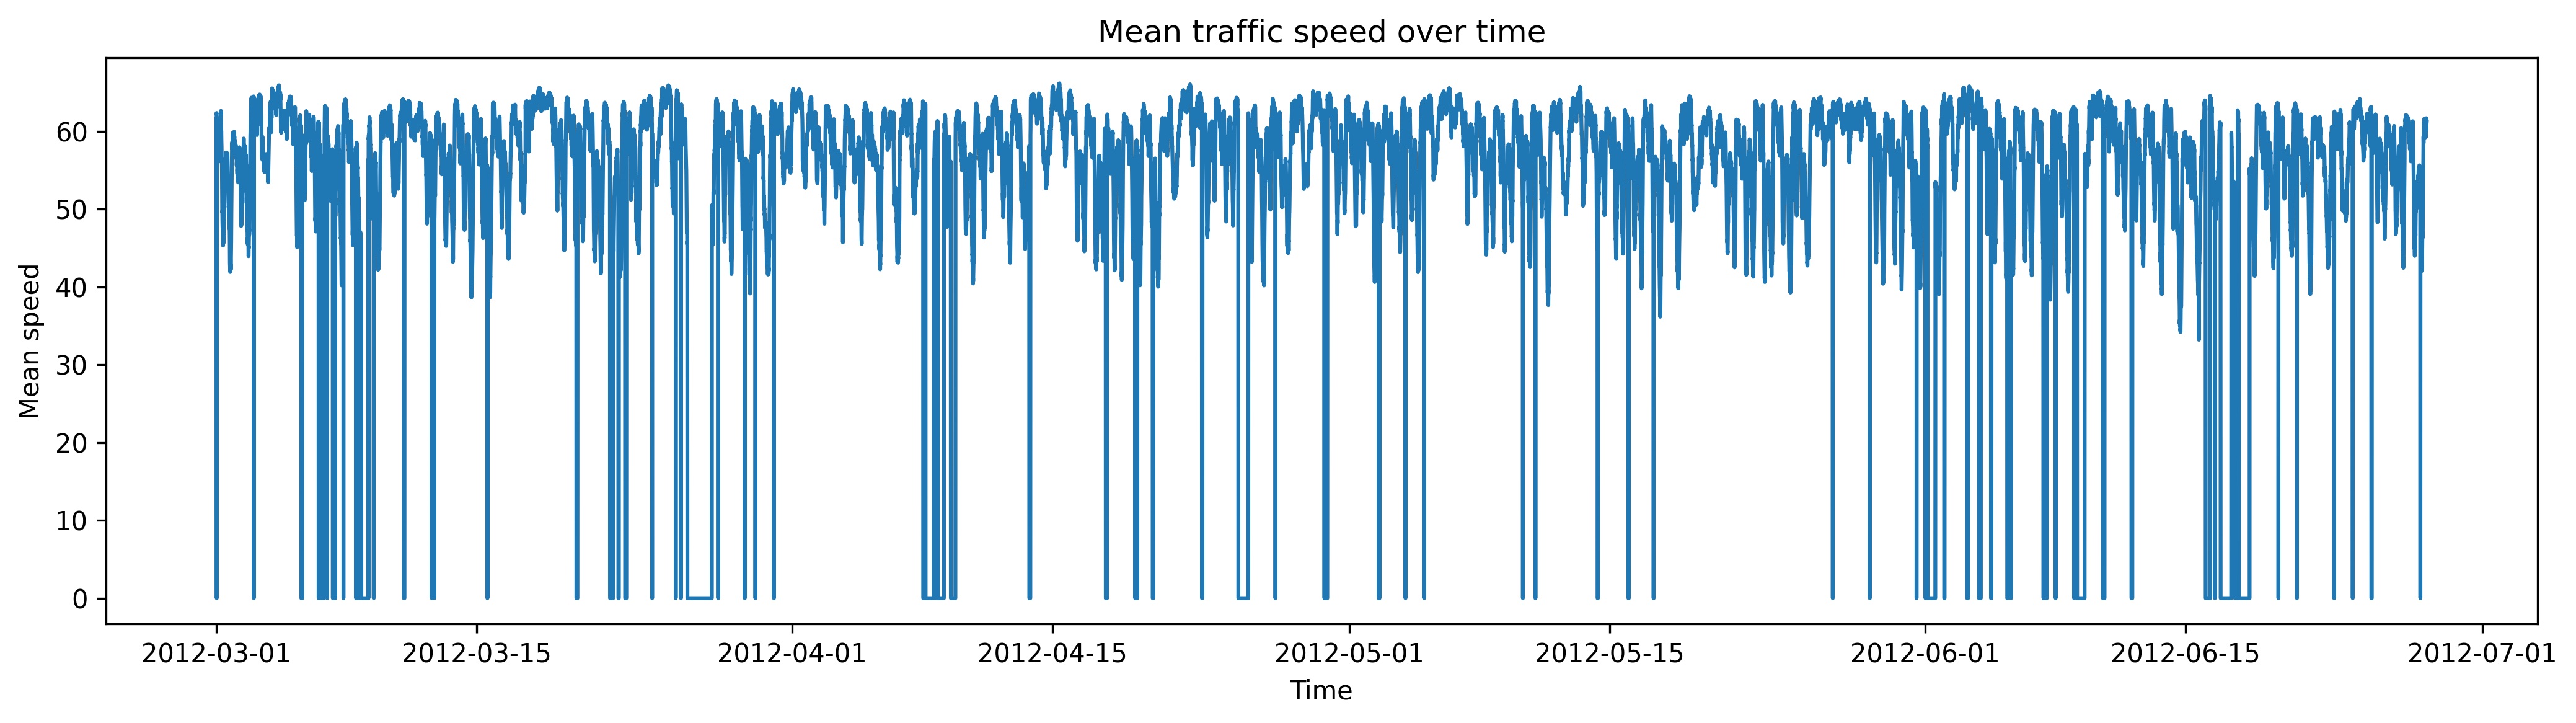
\includegraphics[width=\textwidth]{img/data_analysis/mean_speed_with_zeros}

    \vspace{0.3cm}

    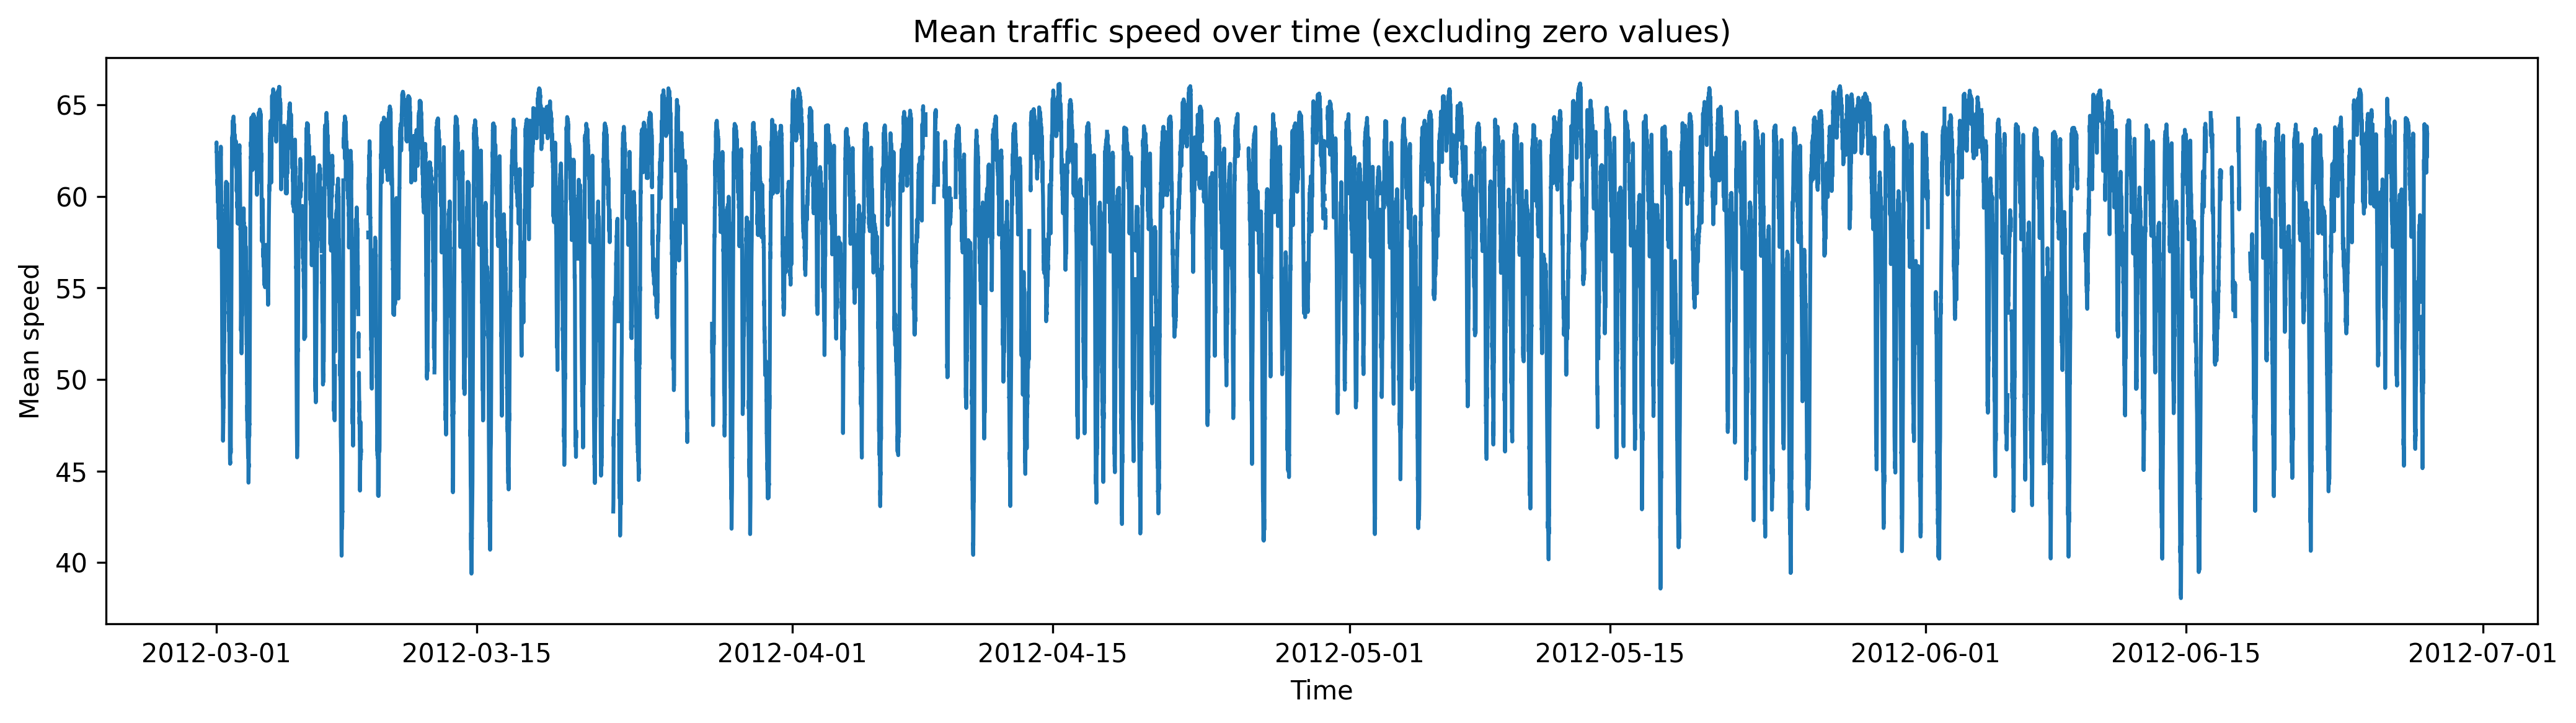
\includegraphics[width=\textwidth]{img/data_analysis/mean_speed_without_zeros}

    \caption{Mean traffic speed over time before (top) and after (bottom) excluding zero values.
    Removing zero-valued measurements eliminates the abrupt drops to zero while preserving the temporal traffic patterns.}
    \label{fig:mean_speed_zero_comparison}
\end{figure}


The valid traffic measurements also exhibit strong temporal structure.
Aggregating traffic speeds by hour of the day reveals a clear daily
seasonality, with average speeds decreasing during typical congestion periods
and increasing again during less congested hours. However, aggregating all
days together partially hides differences between working days and weekends.

Figure~\ref{fig:temporal_patterns} therefore compares the hourly traffic-speed
profiles obtained separately for weekdays and weekends. Weekdays exhibit more
pronounced reductions in average speed during the morning and especially
during the afternoon and evening, whereas weekends show a smoother profile
with generally higher speeds during the corresponding periods. The figure
therefore reveals a weekly component in addition to the daily seasonality.

These observations confirm that the traffic series contains meaningful
temporal dependencies at multiple time scales and motivate the use of a
temporal forecasting model in the subsequent experiments.

\begin{figure}[t]
    \centering
    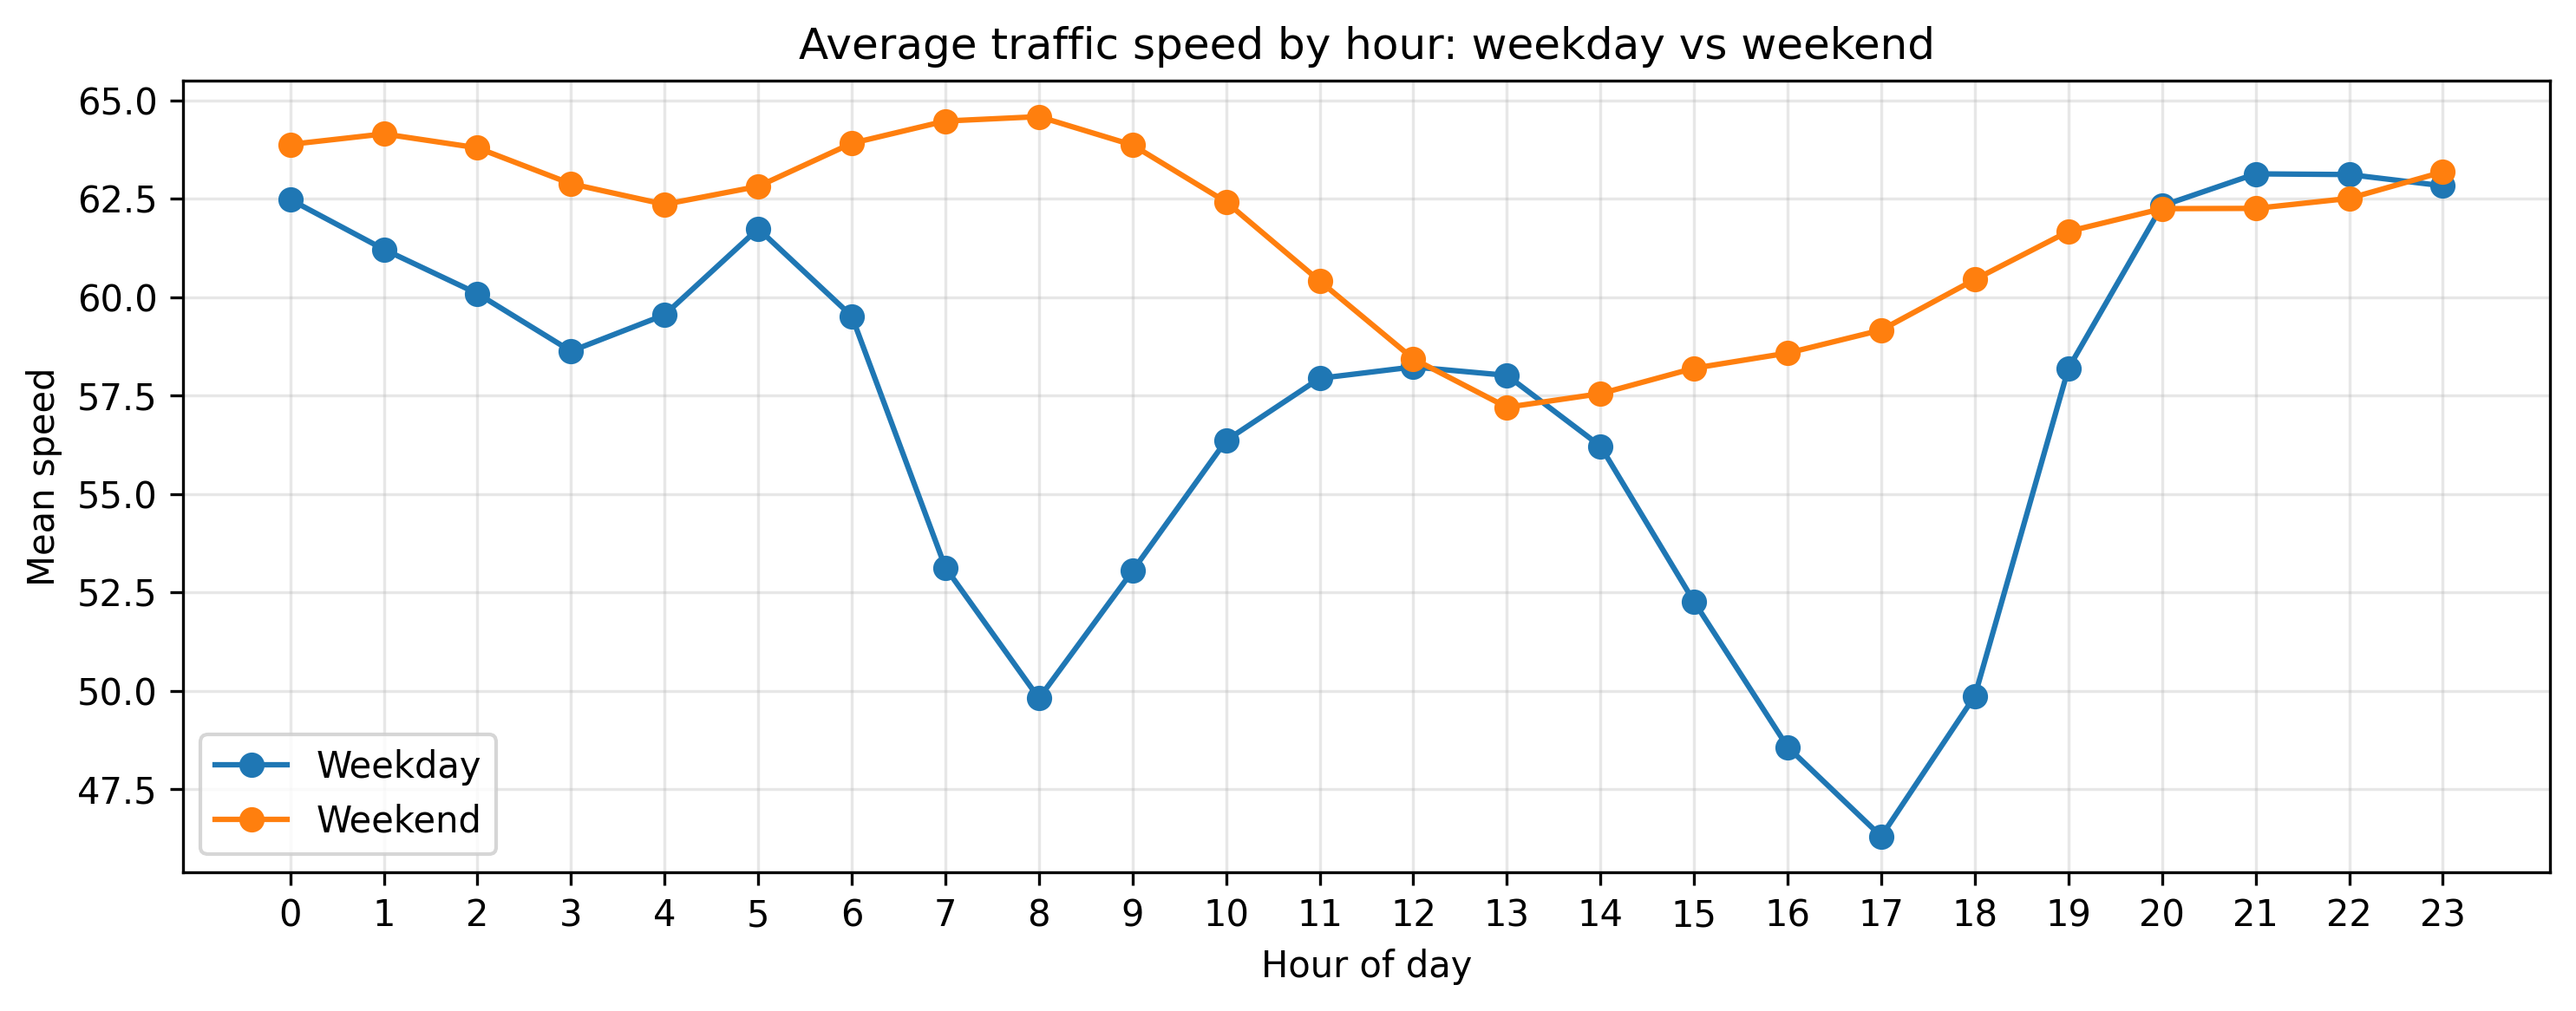
\includegraphics[width=0.75\linewidth]
    {img/data_analysis/weekday_vs_weekend}
    \caption{Average traffic-speed profile by hour of the day, computed
    separately for weekdays and weekends. The different profiles highlight
    both daily and weekly temporal patterns in the METR-LA measurements.}
    \label{fig:temporal_patterns}
\end{figure}

Finally, the distribution of traffic speeds was examined at the individual
sensor level. Considerable heterogeneity was observed across the network, since
the mean traffic speed ranges from approximately 30.89 to 67.73 across
sensors, while the corresponding temporal standard deviations range from
approximately 1.99 to 23.94. Therefore, different sensors exhibit distinct
traffic levels and degrees of variability.

This heterogeneity is particularly relevant for preprocessing, since applying
a single global normalization would ignore the different operating ranges of
individual sensors. For this reason, the normalization strategy described in
Section~\ref{subsec:windowing} estimates separate statistics for each sensor.

Overall, the exploratory analysis identifies two main properties that guide
the preprocessing and modeling choices adopted in this work: a non-negligible
amount of unavailable measurements encoded as zeros, and strong but
heterogeneous temporal traffic patterns across the sensor network.


\subsection{Leakage-Free Data Partitioning}
\label{subsec:splitting}

To preserve the temporal nature of the forecasting problem and prevent
information leakage, the original time series was partitioned
chronologically, without shuffling, into training, validation, and test sets
using a 70\%--10\%--20\% split. Importantly, the partition was performed on
the raw time series before normalization and temporal window construction.

The resulting partitions are summarized in
Table~\ref{tab:chronological_split}. The training set contains 23990
timestamps, followed by 3427 validation timestamps and 6855 test
timestamps. This ordering ensures that validation and test observations
always occur later in time than the observations used for model training.

\begin{table}[t]
    \centering
    \caption{Chronological partition of the original METR-LA time series
    before preprocessing and temporal window construction.}
    \label{tab:chronological_split}
    \begin{tabular}{lrrl}
        \toprule
        Split & Proportion & Timestamps & Time period \\
        \midrule
        Training   & 70\% & 23990 &
        Mar.\ 1 00:00 -- May 23 07:05 \\
        Validation & 10\% & 3427 &
        May 23 07:10 -- Jun.\ 4 04:40 \\
        Test       & 20\% & 6855 &
        Jun.\ 4 04:45 -- Jun.\ 27 23:55 \\
        \bottomrule
    \end{tabular}
\end{table}

All data-dependent preprocessing operations were subsequently fitted using
the training partition only. In particular, the per-sensor normalization
statistics were estimated exclusively from training observations and then
reused unchanged for validation and test data.

Temporal windows were also constructed independently within each partition.
Consequently, an input--target pair can never cross a split boundary. For
example, a training input window cannot use observations from the validation
period as future targets. This procedure preserves the chronological
separation between model development and final evaluation.



\subsection{Missing-Value Handling}
\label{subsec:missing}

Based on the exploratory analysis in
Section~\ref{subsec:eda}, zero-valued traffic measurements were interpreted
as unavailable observations and replaced with missing values before further
processing. Missing values were then handled differently in the input
history and in the forecasting targets, since imputing a target would create
artificial ground-truth values and could bias both training and evaluation.

\paragraph{Input histories.}

Missing observations in the input history were first handled through a
limited interpolation procedure. For each sensor independently, only short
internal gaps of at most three consecutive timestamps were interpolated, and
only when valid observations were available on both sides of the gap. Longer
gaps and missing values at the boundaries of an input window were left
unchanged.

This conservative strategy reduces isolated sensor dropouts while avoiding
the reconstruction of long unavailable periods from potentially unrelated
observations. Before interpolation, missing values accounted for
approximately 7.13\%, 7.00\%, and 12.13\% of the input values in the
training, validation, and test windows, respectively. After short-gap
interpolation, these proportions decreased to approximately 6.85\%, 6.83\%,
and 11.92\%.

Therefore, interpolation only
moderately reduces the overall amount of missing data. This is expected
because the procedure deliberately targets short internal gaps while
preserving longer periods of sensor unavailability.

Input windows for which all sensors were unavailable throughout the complete
history were removed, since they contain no temporal information from which a
forecast can be produced. In contrast, a window was retained when only a
subset of sensors was fully unavailable, because observations from the
remaining sensors may still provide useful information, particularly for the
graph-temporal model.

After this filtering step, residual missing input values were replaced by
zero in the standardized domain. Since normalization is performed separately
for each sensor using training statistics, this value corresponds to the
training mean of that sensor rather than to a physical traffic speed of zero.
An input availability mask was retained to distinguish observed from missing
measurements.

\paragraph{Forecasting targets.}

A stricter policy was adopted for the forecasting targets. Target values were
never interpolated or semantically imputed, since doing so would introduce
synthetic ground truth into the optimization and evaluation procedures.
Instead, a binary target-availability mask was constructed and propagated
throughout the complete pipeline.

Windows with no valid target observations over the complete forecasting
period were removed. Partially observed target windows were retained, while
missing target entries were numerically replaced with finite placeholder
values only to maintain valid tensor representations. These entries were
always excluded from the loss and evaluation metrics through the target
mask and therefore never contributed to model optimization or reported
performance.

After filtering fully unavailable input and target windows, the final dataset
contains 22817 training samples, 3240 validation samples, and 6224 test
samples, as reported in Table~\ref{tab:final_dataset}. Despite the missing
periods identified in the raw data, target availability remains above 94\%
at all evaluated horizons, providing a sufficiently large set of valid
observations for model training and evaluation.

\begin{table}[t]
    \centering
    \caption{Number of temporal samples retained after missing-data
    processing and filtering.}
    \label{tab:final_dataset}
    \begin{tabular}{lr}
        \toprule
        Split & Final samples \\
        \midrule
        Training   & 22817 \\
        Validation & 3240 \\
        Test       & 6224 \\
        \bottomrule
    \end{tabular}
\end{table}

Target availability nevertheless remains high at all evaluated horizons,
ranging from approximately 94\% to 97\% depending on the split and forecast
horizon.


\subsection{Normalization and Temporal Windowing}
\label{subsec:windowing}

As discussed in Section~\ref{subsec:eda}, traffic-speed distributions vary
substantially across sensors. For this reason, the data were standardized
independently for each sensor rather than using global statistics shared
across the complete network.

For each sensor $n$, the mean $\mu_n$ and standard deviation $\sigma_n$ were
estimated exclusively from the valid observations in the training partition.
Each available traffic-speed observation $x_{t,n}$ was then transformed as

\begin{equation}
    \tilde{x}_{t,n}
    =
    \frac{x_{t,n}-\mu_n}{\sigma_n}.
    \label{eq:normalization}
\end{equation}

The same training statistics were subsequently applied without modification
to the validation and test partitions. This prevents information from future
partitions from influencing the preprocessing procedure.

After preprocessing and normalization, each chronological partition was
independently transformed into input--target pairs using a sliding-window
procedure. Given an input-history length $H=12$ and a forecasting window
$F=12$, a sample generated at time $t$ consists of the previous 12 traffic
observations and the following 12 observations to be predicted.

More formally, the input and target windows are defined as

\begin{equation}
    \mathbf{X}_t
    =
    \left[
        \tilde{\mathbf{x}}_{t-H+1},
        \ldots,
        \tilde{\mathbf{x}}_{t}
    \right]
    \in \mathbb{R}^{H \times N},
    \label{eq:input_window}
\end{equation}

and

\begin{equation}
    \mathbf{Y}_t
    =
    \left[
        \tilde{\mathbf{x}}_{t+1},
        \ldots,
        \tilde{\mathbf{x}}_{t+F}
    \right]
    \in \mathbb{R}^{F \times N},
    \label{eq:target_window}
\end{equation}

where $N=207$ is the number of sensors. Since measurements are sampled every
five minutes, both $H=12$ and $F=12$ correspond to one hour of traffic
observations.


Although the models jointly predict all $F=12$ future steps, the main
evaluation is performed at three representative forecasting horizons:
$t+3$, $t+6$, and $t+12$, corresponding respectively to 15, 30, and
60 minutes into the future. This allows performance to be analyzed as the
forecasting task becomes progressively more difficult with increasing
prediction horizon.


The windowing procedure was applied jointly to the traffic values and their
availability masks. Consequently, each input window is associated with an
input mask indicating which historical observations are available, while
each target window is associated with a target mask identifying the entries
that can contribute to the training loss and evaluation metrics.

Partially observed windows are therefore retained whenever useful information
is available, rather than being discarded entirely because of a small number
of missing sensor measurements. As described in
Section~\ref{subsec:missing}, unavailable target entries never contribute to
model optimization or performance evaluation.


The resulting preprocessing pipeline therefore preserves the chronological
structure of the forecasting problem, estimates all data-dependent
transformations exclusively from the training period, and explicitly tracks
unavailable observations through masks. The same processed input--target
windows are used by all forecasting approaches described in the following
section, ensuring that differences in performance are attributable to the
forecasting models rather than to different data-processing procedures.
%\section{Forecasting Methodology}
\label{sec:methodology}

\subsection{Probabilistic Forecasting Formulation}
\label{subsec:probabilistic}

The forecasting task is formulated probabilistically through conditional
quantile estimation. Rather than predicting a single future traffic speed,
the neural forecasting models estimate three quantiles for each sensor and
forecasting step,

\begin{equation}
    \mathcal{Q} = \{0.1, 0.5, 0.9\}.
    \label{eq:quantiles}
\end{equation}

For an input window $\mathbf{X}_t$, the models therefore produce

\begin{equation}
    \hat{\mathbf{Y}}_t
    \in
    \mathbb{R}^{F \times N \times |\mathcal{Q}|},
    \label{eq:probabilistic_output}
\end{equation}

where $F=12$ is the forecasting window, $N=207$ is the number of sensors,
and $|\mathcal{Q}|=3$ is the number of predicted quantiles.

The median prediction $\hat{y}^{(0.5)}$ is used as the point forecast when
computing deterministic metrics such as MAE and RMSE. The lower and upper
quantiles define the predictive interval

\begin{equation}
    \left[
        \hat{y}^{(0.1)},
        \hat{y}^{(0.9)}
    \right],
    \label{eq:prediction_interval}
\end{equation}

which has a nominal coverage probability of $80\%$. This formulation makes it
possible to evaluate point forecasting accuracy and predictive uncertainty
using a single model.


The models are trained using the Pinball Loss. For a target value $y$, a
predicted quantile $\hat{y}^{(q)}$, and a quantile level $q$, the loss is
defined as

\begin{equation}
    \mathcal{L}_{q}
    \left(y,\hat{y}^{(q)}\right)
    =
    \max
    \left(
        q\left(y-\hat{y}^{(q)}\right),
        (q-1)\left(y-\hat{y}^{(q)}\right)
    \right).
    \label{eq:pinball_loss}
\end{equation}

Unlike a symmetric regression loss, the Pinball Loss penalizes
underestimation and overestimation differently according to the target
quantile. Minimizing it therefore allows the model to estimate different
regions of the conditional target distribution rather than only its central
value.


Since some target observations are unavailable, the Pinball Loss is computed
only over valid target entries. During training, consider a mini-batch of
$B$ samples. Let $b \in \{1,\ldots,B\}$ denote the sample index,
$h \in \{1,\ldots,F\}$ the forecast step, and
$n \in \{1,\ldots,N\}$ the sensor index. The binary mask
$m_{b,h,n} \in \{0,1\}$ indicates whether the corresponding target value is
available.

For each mini-batch, the training loss is obtained by averaging the Pinball
Loss over all valid target entries and over all predicted quantiles:

\begin{equation}
    \mathcal{L}_{\mathrm{masked}}
    =
    \frac{
        \displaystyle
        \sum_{b=1}^{B}
        \sum_{h=1}^{F}
        \sum_{n=1}^{N}
        m_{b,h,n}
        \sum_{q\in\mathcal{Q}}
        \mathcal{L}_{q}
        \left(
            y_{b,h,n},
            \hat{y}_{b,h,n}^{(q)}
        \right)
    }{
        \displaystyle
        |\mathcal{Q}|
        \sum_{b=1}^{B}
        \sum_{h=1}^{F}
        \sum_{n=1}^{N}
        m_{b,h,n}
    }.
    \label{eq:masked_pinball}
\end{equation}

Consequently, unavailable target values do not contribute to the loss,
while every valid target contributes once for each quantile in
$\mathcal{Q}$. This is consistent with the missing-data strategy described
in Section~\ref{subsec:missing}.


\subsection{Persistence Baseline}
\label{subsec:persistence}

A persistence model is used as the simplest forecasting baseline. For each
sensor, the value at the final time step of the input window is repeated
across the complete forecasting horizon. The prediction for sensor $n$ at
any future step $h$ is therefore

\begin{equation}
    \hat{y}_{t+h,n} = x_{t,n},
    \qquad h=1,\ldots,F.
    \label{eq:persistence}
\end{equation}

The persistence baseline contains no trainable parameters and does not
explicitly model either temporal dynamics or spatial interactions. It
therefore provides a simple reference for determining whether the learned
models extract useful predictive information from the historical traffic
sequence.


\subsection{Temporal GRU}
\label{subsec:gru}

The first learned forecasting model is a temporal GRU designed to capture
temporal dependencies without exploiting the sensor graph. Each sensor is
processed independently using its own sequence of historical traffic
observations, while the GRU parameters are shared across all sensors.

For a given sensor $n$, the input sequence

\begin{equation}
    \left[
        \tilde{x}_{t-H+1,n},
        \ldots,
        \tilde{x}_{t,n}
    \right]
\end{equation}

is processed by the same recurrent network. No information from other
sensors is exchanged during the forward pass. The model therefore provides a
controlled no-graph baseline against which the contribution of spatial
message passing can be evaluated.

The selected temporal architecture consists of a two-layer GRU with hidden
dimension 64. The final hidden representation of each sensor is passed to a
linear output layer that jointly predicts all $F=12$ future steps and all
three quantiles. For each sensor, the output layer therefore produces

\begin{equation}
    F \times |\mathcal{Q}| = 12 \times 3 = 36
\end{equation}

values, which are reshaped into the corresponding forecast-step and quantile
dimensions.

The complete model contains 40164 trainable parameters. Because the same
network is applied to every sensor, the parameter count does not scale with
the number of nodes in the traffic network.


\subsection{Graph Representation and Diffusion Message Passing}
\label{subsec:graph}

Spatial dependencies are introduced through the sensor graph provided with
METR-LA. Each traffic sensor corresponds to a graph node, while the adjacency
matrix

\begin{equation}
    \mathbf{A} \in \mathbb{R}^{N \times N}
\end{equation}

encodes directed, weighted connections between sensors. Throughout this work,
the convention is that $A_{ij}$ represents the weight assigned at node $i$
to the message received from node $j$. Therefore, row $i$ contains the
weights used to aggregate information into node $i$.

The provided adjacency matrix already contains self-connections. Therefore,
no additional identity matrix is added to $\mathbf{A}$ before normalization.
This avoids introducing artificial self-loops or modifying the relative
weights of the graph supplied with the dataset.

Before message passing, the adjacency matrix is row-normalized as

\begin{equation}
    \mathbf{P} = \mathbf{D}^{-1}\mathbf{A},
    \label{eq:row_normalization}
\end{equation}

where $\mathbf{D}$ is the diagonal matrix of row sums,

\begin{equation}
    D_{ii} = \sum_j A_{ij}.
\end{equation}

Under the adopted convention, the one-step propagated representation of node
$i$ is therefore

\begin{equation}
    (\mathbf{P}\mathbf{X})_i
    =
    \sum_j P_{ij}\mathbf{X}_j,
    \label{eq:graph_aggregation}
\end{equation}

so that node $i$ receives a weighted combination of the representations of
the nodes $j$ connected to it.

Spatial information is propagated through a diffusion-style message-passing
layer. Given node features $\mathbf{X}$, the layer computes

\begin{equation}
    \mathbf{H}
    =
    \sum_{k=0}^{K}
    \mathbf{P}^{k}\mathbf{X}\mathbf{W}_{k}
    +
    \mathbf{b},
    \label{eq:diffusion}
\end{equation}

where $K$ controls the maximum diffusion depth and each $\mathbf{W}_{k}$ is
a learnable projection associated with a different propagation step. The
$k=0$ term, for which $\mathbf{P}^{0}=\mathbf{I}$, directly preserves the
node's own representation, while the terms with $k\geq1$ incorporate
information propagated through the graph.

For the main configuration, $K=2$, yielding

\begin{equation}
    \mathbf{H}
    =
    \mathbf{X}\mathbf{W}_{0}
    +
    \mathbf{P}\mathbf{X}\mathbf{W}_{1}
    +
    \mathbf{P}^{2}\mathbf{X}\mathbf{W}_{2}
    +
    \mathbf{b}.
    \label{eq:diffusion_k2}
\end{equation}

The first term provides an explicit transformation of each node's own
representation, while the remaining terms incorporate information propagated
over one and two graph transitions. Since the diagonal entries already
present in $\mathbf{A}$ are preserved by the row normalization, the
one-step and two-step diffusion terms may themselves also contain
self-information.


\subsection{Graph-Temporal Architecture}
\label{subsec:graph_temporal}

The main forecasting model combines the diffusion operation described in
Section~\ref{subsec:graph} with recurrent temporal modeling. The architecture
is composed of two consecutive graph-temporal blocks. Each block first
propagates information between sensors through diffusion message passing and
then applies a GRU to model the temporal evolution of the resulting node
representations (Figure \ref{fig:graphtemporalarchitecture}).

Given an input window, diffusion is applied independently at each temporal
step, allowing every sensor representation to incorporate information from
its graph neighborhood. The resulting sequence of spatial representations is
then processed by a GRU independently for each node, with recurrent
parameters shared across sensors. The first block preserves the complete
temporal sequence so that it can be processed by the second diffusion--GRU
block.

The final temporal representation is passed to a linear probabilistic head
that directly predicts the 12 future steps for the three quantile levels
defined in Section~\ref{subsec:probabilistic}. As in the Temporal GRU, the
complete forecasting window is generated in a single forward pass rather
than recursively feeding previous predictions back into the model.

The selected graph-temporal model uses a graph hidden dimension of 64, a GRU
hidden dimension of 64, one GRU layer per graph-temporal block, two
graph-temporal blocks, and a diffusion depth of $K=2$. The complete
architecture contains 64868 trainable parameters.

\begin{figure}[t]
    \centering
    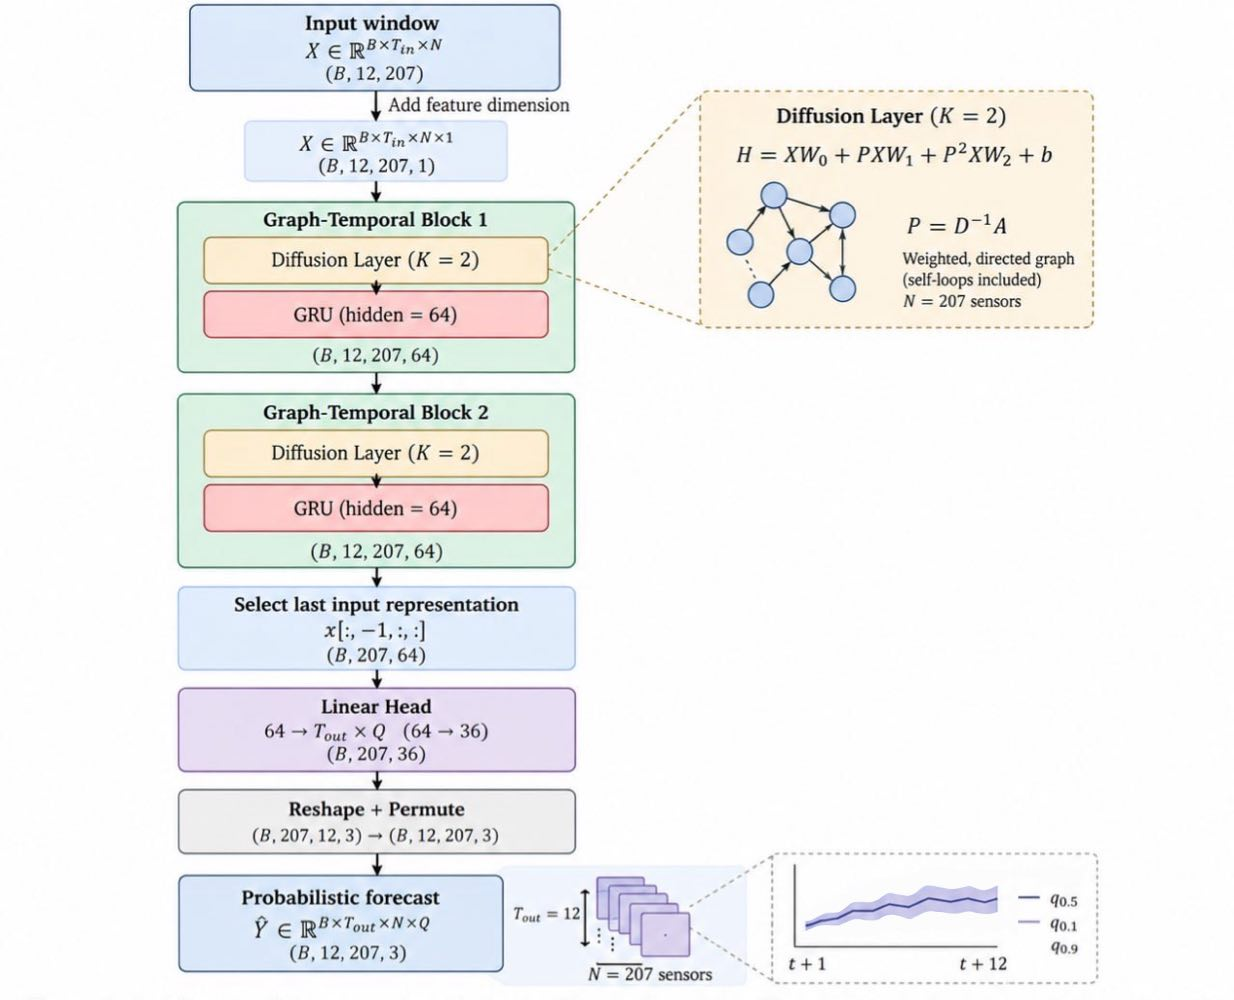
\includegraphics[width=\linewidth]{img/graphtemporalarchitecture}
    \caption{Architecture of the proposed graph-temporal forecasting model.}
    \label{fig:graphtemporalarchitecture}
\end{figure}
%\section{Experimental Setup}
\label{sec:experimental_setup}

\subsection{Training Protocol}
\label{subsec:training}

Both the Temporal GRU and the Graph-Temporal model were trained using the
masked Pinball Loss defined in Equation~\ref{eq:masked_pinball}. Model
parameters were optimized with Adam using mini-batches of 64 samples.

Training was performed for a maximum of 200 epochs with early stopping based
on the validation Pinball Loss and a patience of 10 epochs. Whenever the
validation loss improved, the corresponding model checkpoint was retained.
Training was terminated if no further improvement was observed for 10
consecutive epochs, and the checkpoint associated with the lowest validation
loss was used for subsequent evaluation.

Both neural models use direct multi-horizon forecasting: all 12 future time
steps and the three target quantiles are predicted simultaneously from the
input history.

No test-set information was used for hyperparameter selection, early stopping,
or model calibration. The test partition was accessed only after the model
configuration had been selected using the training and validation partitions.


\subsection{Hyperparameter Selection}
\label{subsec:hyperparameters}

Hyperparameters were selected exclusively according to the validation
Pinball Loss. Separate grid searches were performed for the Temporal GRU and
the Graph-Temporal model, since the two architectures expose different
model-specific parameters. The search spaces and selected configurations are
summarized in Table~\ref{tab:hyperparameters}.

\begin{table}[t]
    \centering
    \caption{Hyperparameter search spaces and selected configurations for the
    two neural forecasting models.}
    \label{tab:hyperparameters}
    \begin{tabular}{lll}
        \toprule
        Model & Hyperparameter & Values \\
        \midrule

        Temporal GRU
        & Hidden dimension & $\{32,\mathbf{64}\}$ \\
        & GRU layers & $\{1,\mathbf{2}\}$ \\
        & Learning rate & $\{\mathbf{5\times10^{-4}},10^{-3}\}$ \\
        \midrule

        Graph-Temporal
        & Graph hidden dimension & $\{32,\mathbf{64}\}$ \\
        & GRU hidden dimension & $\mathbf{64}$ \\
        & GRU layers per block & $\{\mathbf{1},2\}$ \\
        & Learning rate & $\{\mathbf{5\times10^{-4}},10^{-3}\}$ \\
        & Diffusion depth $K$ & $\mathbf{2}$ \\
        & Graph-temporal blocks & $\mathbf{2}$ \\
        \bottomrule
    \end{tabular}
\end{table}

Selected values are highlighted in bold. The diffusion depth and number of
graph-temporal blocks were kept fixed during the main hyperparameter search;
the effect of changing the diffusion depth is investigated separately in
Section~\ref{subsec:diffusion_depth}.

For the Temporal GRU, the selected configuration uses a hidden dimension of
64, two recurrent layers, and a learning rate of $5\times10^{-4}$. The best
checkpoint was obtained at epoch 78, with a validation Pinball Loss of
0.1240.

For the Graph-Temporal model, the selected configuration uses a graph hidden
dimension of 64, a GRU hidden dimension of 64, one recurrent layer per
graph-temporal block, and a learning rate of $5\times10^{-4}$. With two
blocks and diffusion depth $K=2$, the best checkpoint was obtained at epoch
106, reaching a validation Pinball Loss of 0.1133.


The learning curves of the selected configurations are shown in
Figure~\ref{fig:learning_curves}. For both models, the training loss decreases
progressively, while the validation loss eventually reaches a minimum and
ceases to improve. The selected checkpoints therefore correspond to the
minimum validation loss rather than to the final training epoch, consistently
with the early-stopping procedure described in
Section~\ref{subsec:training}.

\begin{figure}[t]
    \centering

    \begin{subfigure}[b]{0.48\linewidth}
        \centering
        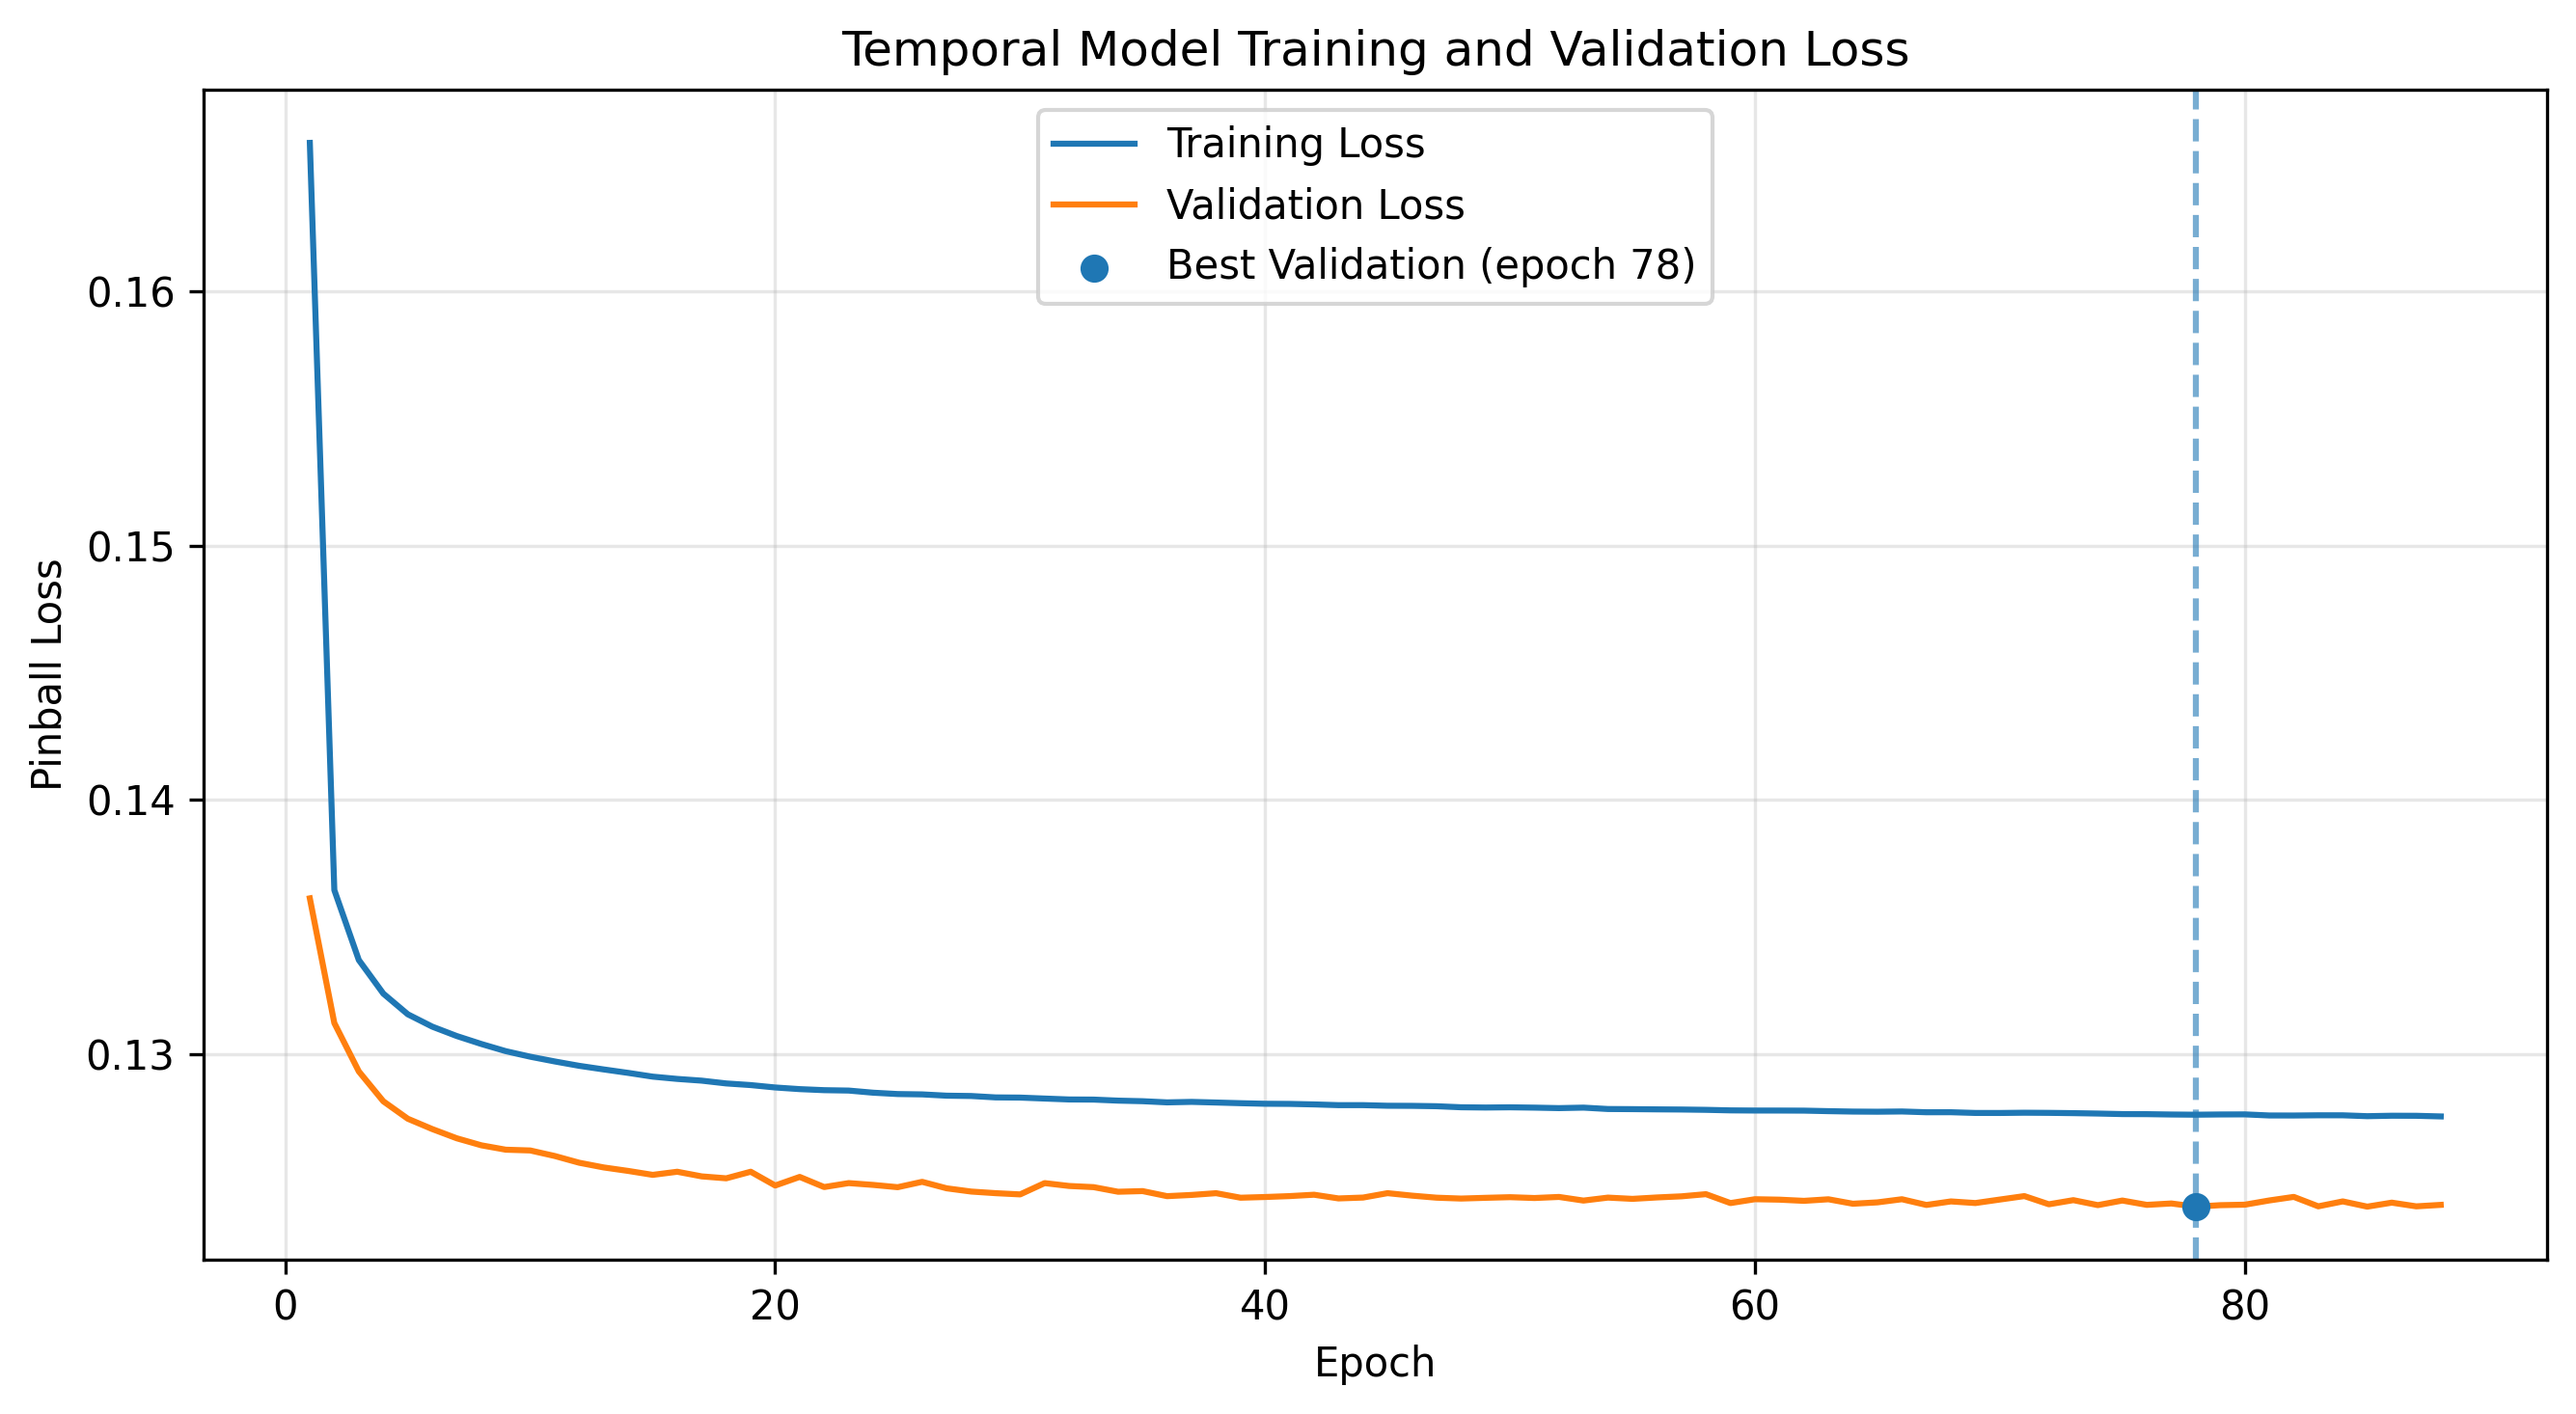
\includegraphics[width=\linewidth]{img/temporal_gru/learning_curves}
        \caption{Temporal GRU.}
        \label{fig:gru_learning_curve}
    \end{subfigure}
    \hfill
    \begin{subfigure}[b]{0.48\linewidth}
        \centering
        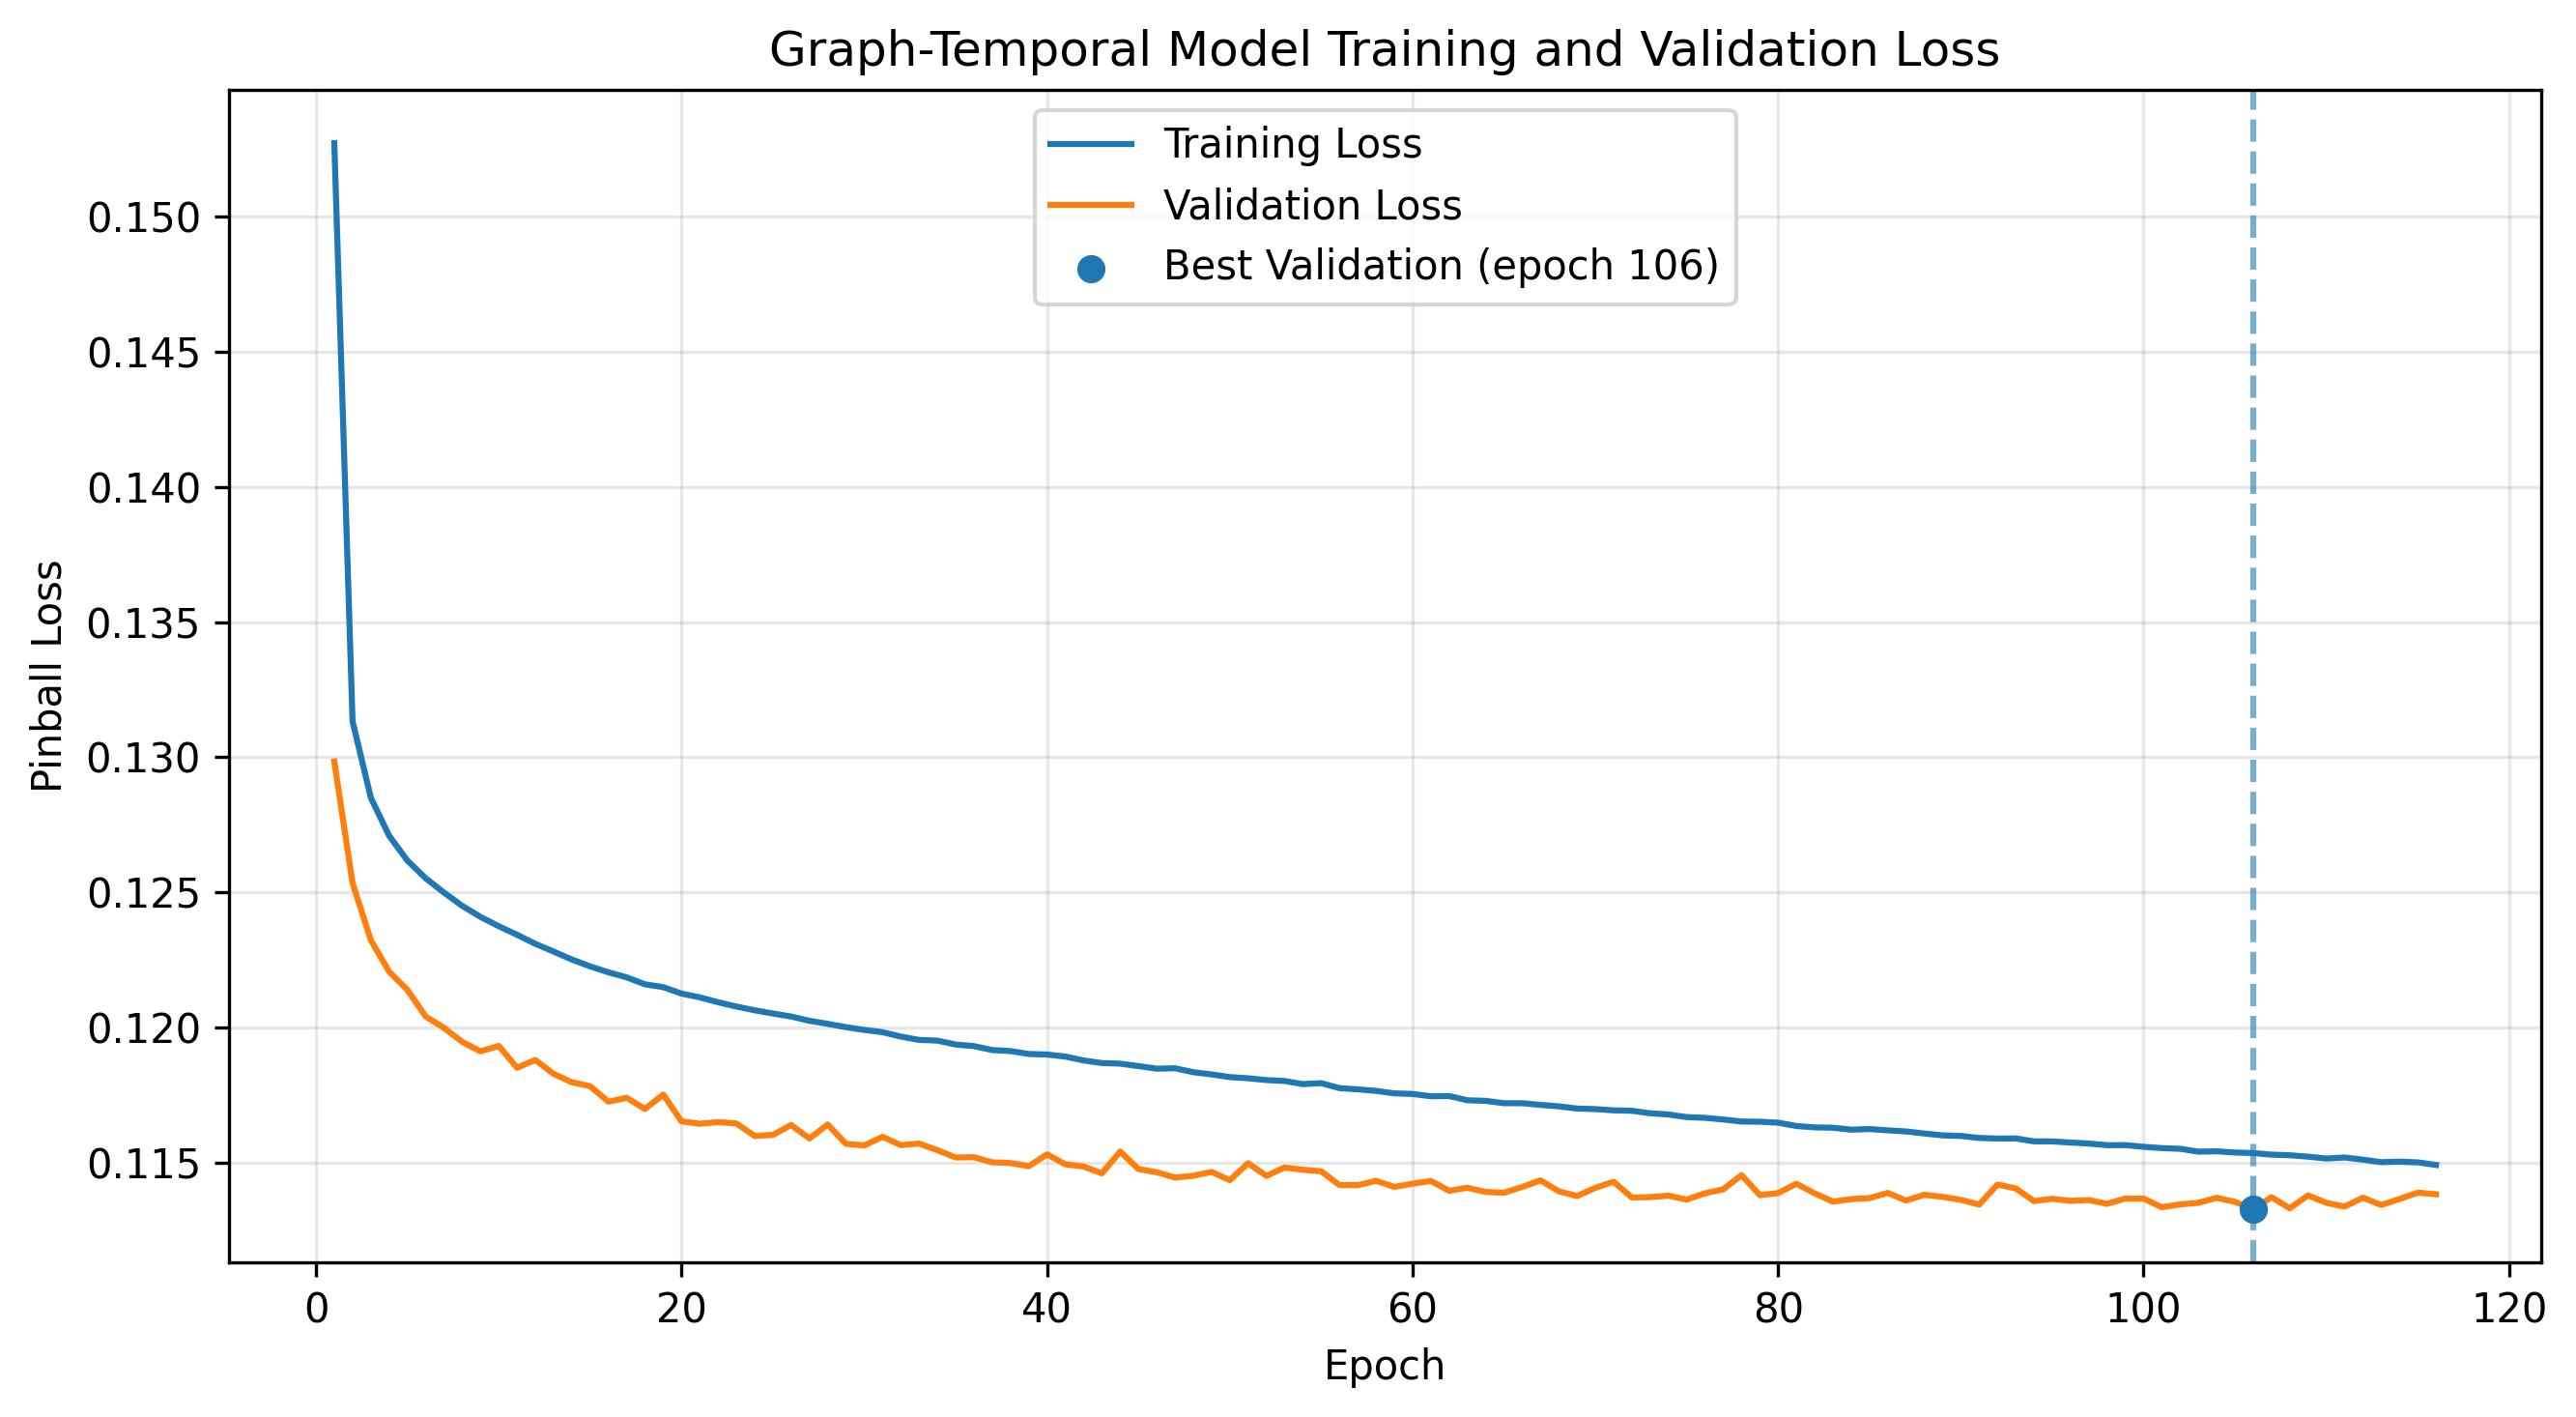
\includegraphics[width=\linewidth]{img/graph_temporal/graph_temporal_learning_curves}
        \caption{Graph-Temporal model.}
        \label{fig:graph_learning_curve}
    \end{subfigure}

    \caption{Training and validation Pinball Loss for the selected model
    configurations.}
    \label{fig:learning_curves}
\end{figure}

Validation Pinball Loss was used as the single model-selection criterion
rather than selecting configurations directly according to empirical
coverage. This criterion evaluates the quality of the predicted quantiles
without optimizing the model specifically for a single coverage statistic.
Coverage and interval width were instead retained as complementary
reliability metrics for the final analysis.


\subsection{Evaluation Metrics}
\label{subsec:metrics}

Performance is evaluated at the three forecasting horizons of 15, 30, and 60 minutes. All metrics are
computed only over valid target observations using the corresponding target
availability mask.

Point forecasting accuracy is evaluated using the median prediction
$\hat{y}^{(0.5)}$. The Mean Absolute Error (MAE) is defined as

\begin{equation}
    \mathrm{MAE}
    =
    \frac{1}{|\Omega|}
    \sum_{i\in\Omega}
    \left|
        y_i-\hat{y}^{(0.5)}_i
    \right|,
    \label{eq:mae}
\end{equation}

where $\Omega$ denotes the set of valid target entries at the considered
forecast horizon.

The Root Mean Squared Error (RMSE) is defined as

\begin{equation}
    \mathrm{RMSE}
    =
    \sqrt{
        \frac{1}{|\Omega|}
        \sum_{i\in\Omega}
        \left(
            y_i-\hat{y}^{(0.5)}_i
        \right)^2
    }.
    \label{eq:rmse}
\end{equation}

While MAE measures the average magnitude of the forecasting error, RMSE
assigns greater weight to large deviations and is therefore useful for
identifying models that occasionally produce particularly inaccurate
forecasts.

Probabilistic forecasting quality is evaluated through the Pinball Loss
introduced in Equation~\ref{eq:pinball_loss}. The loss is reported
separately for $q_{0.1}$, $q_{0.5}$, and $q_{0.9}$, allowing the quality of
the lower, median, and upper conditional quantile estimates to be examined
individually.

The reliability of the predictive intervals is assessed through empirical
coverage. For the nominal 80\% interval
$[\hat{y}^{(0.1)},\hat{y}^{(0.9)}]$, coverage is computed as

\begin{equation}
    \mathrm{Coverage}
    =
    \frac{1}{|\Omega|}
    \sum_{i\in\Omega}
    \mathbb{I}
    \left[
        \hat{y}^{(0.1)}_i
        \leq y_i
        \leq
        \hat{y}^{(0.9)}_i
    \right],
    \label{eq:coverage}
\end{equation}

where $\mathbb{I}[\cdot]$ is the indicator function. A well-calibrated
80\% predictive interval is expected to contain approximately 80\% of the
observed targets.

Coverage alone is not sufficient to characterize forecast quality, since
arbitrarily wide intervals could achieve high coverage. Predictive sharpness
is therefore evaluated using the mean interval width,

\begin{equation}
    \mathrm{Width}
    =
    \frac{1}{|\Omega|}
    \sum_{i\in\Omega}
    \left(
        \hat{y}^{(0.9)}_i
        -
        \hat{y}^{(0.1)}_i
    \right).
    \label{eq:interval_width}
\end{equation}

Coverage and interval width are interpreted jointly: reliable forecasts
should achieve coverage close to the nominal level while keeping predictive
intervals as informative as possible.

Finally, the quantile crossing rate measures the fraction of predictions for
which the estimated quantiles violate their expected ordering,

\begin{equation}
    \hat{y}^{(0.1)}
    \leq
    \hat{y}^{(0.5)}
    \leq
    \hat{y}^{(0.9)}.
\end{equation}

A crossing rate close to zero indicates that the independently predicted
quantiles are almost always ordered consistently.

In addition to these scalar metrics, calibration plots are used to compare
the nominal quantile levels with their empirical frequencies. This provides
a more detailed view of probabilistic calibration than the 80\% interval
coverage alone.


\subsection{Hardware and Reproducibility}
\label{subsec:hardware}

All neural models were implemented in PyTorch and trained using an NVIDIA
GeForce RTX 4060 Laptop GPU with CUDA acceleration. A fixed random seed of
42 was used throughout the experiments to improve reproducibility.

Model checkpoints corresponding to the best validation Pinball Loss were
saved during training and subsequently reloaded for final evaluation. The
same preprocessing pipeline, dataset partitions, forecast horizons, and
evaluation functions were used across the learned models to ensure a
consistent experimental comparison.
%\section{In-Distribution Forecasting Results}
\label{sec:in_distribution_results}


\subsection{Point Forecasting Performance}
\label{subsec:point_results}

The point forecasting performance of the three models is reported in
Table~\ref{tab:point_results}. For the two probabilistic neural models, the
median prediction $q_{0.5}$ is used as the point forecast. As expected,
forecasting accuracy decreases as the prediction horizon increases, with
both MAE and RMSE increasing from 15 to 60 minutes for all models.

\begin{table}[t]
    \centering
    \caption{Point forecasting performance on the test set at the three
    forecasting horizons. The best result for each metric and horizon is
    highlighted in bold.}
    \label{tab:point_results}
    \begin{tabular}{llccc}
        \toprule
        & & \multicolumn{3}{c}{Forecast horizon} \\
        \cmidrule(lr){3-5}
        Model & Metric & 15 min & 30 min & 60 min \\
        \midrule

        Persistence
        & MAE  & 3.501 & 4.199 & 5.351 \\
        & RMSE & 6.411 & 8.023 & 10.279 \\
        \midrule

        Temporal GRU
        & MAE  & 3.080 & 3.735 & 4.733 \\
        & RMSE & 6.081 & 7.548 & 9.411 \\
        \midrule

        Graph-Temporal
        & MAE  & \textbf{2.901} & \textbf{3.442} & \textbf{4.244} \\
        & RMSE & \textbf{5.511} & \textbf{6.758} & \textbf{8.378} \\
        \bottomrule
    \end{tabular}
\end{table}

The Persistence baseline exhibits the largest errors at all forecasting
horizons. Introducing temporal modeling through the GRU consistently improves
over persistence, showing that the recent history contains temporal patterns
that cannot be captured by simply propagating the final input value into the
future.

The Graph-Temporal model further reduces both MAE and RMSE at every horizon.
Compared with the Temporal GRU, the MAE decreases from 3.080 to 2.901 at
15 minutes, from 3.735 to 3.442 at 30 minutes, and from 4.733 to 4.244 at
60 minutes. These correspond to relative reductions of approximately
5.8\%, 7.8\%, and 10.3\%, respectively. The corresponding RMSE reductions
are approximately 9.4\%, 10.5\%, and 11.0\%.

The improvement introduced by the graph component becomes more pronounced
as the forecasting horizon increases. This suggests that spatial information
is particularly useful for longer-term predictions, where the future state
of a sensor becomes increasingly difficult to estimate from its own temporal
history alone. The reduction in RMSE is also consistently larger than the
reduction in MAE, indicating that the Graph-Temporal model is particularly
effective in reducing larger forecasting errors.

The same trend is illustrated in
Figure~\ref{fig:point_performance}, where the performance gap between the
Temporal GRU and the Graph-Temporal model becomes progressively larger toward
the 60-minute horizon.

\begin{figure}[t]
    \centering

    \begin{minipage}[b]{0.48\linewidth}
        \centering
        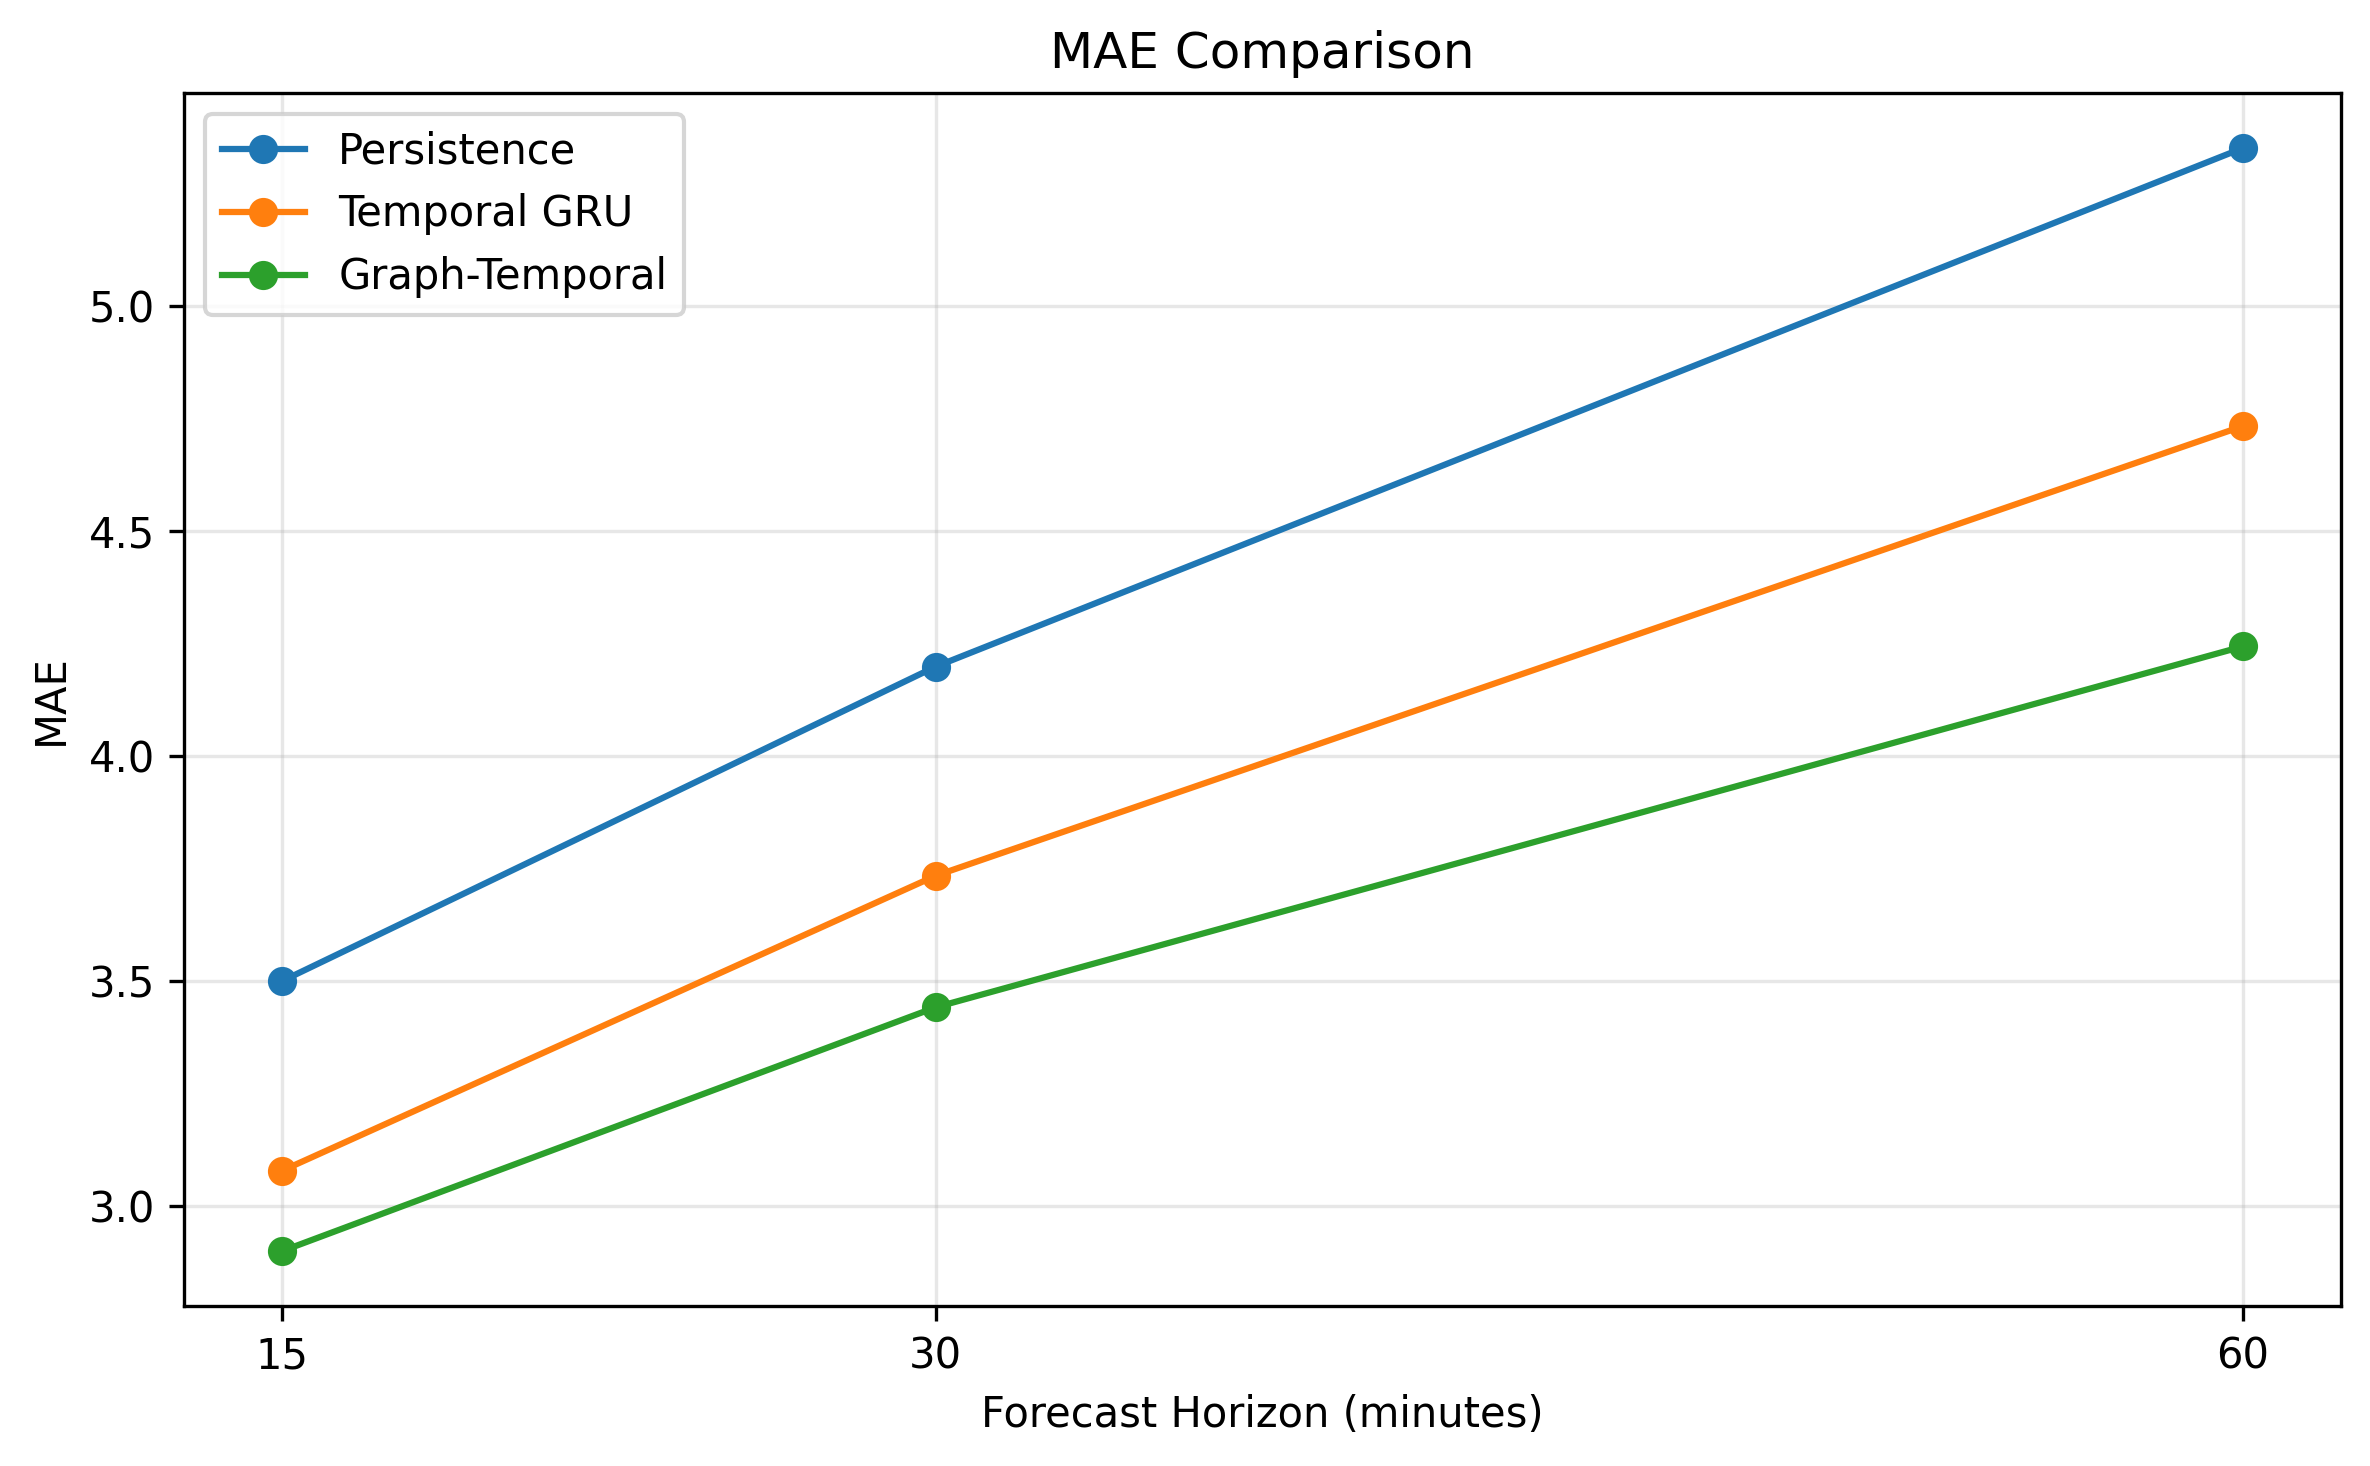
\includegraphics[width=\linewidth]{img/model_comparison/mae_model_comparison}
    \end{minipage}
    \hfill
    \begin{minipage}[b]{0.48\linewidth}
        \centering
        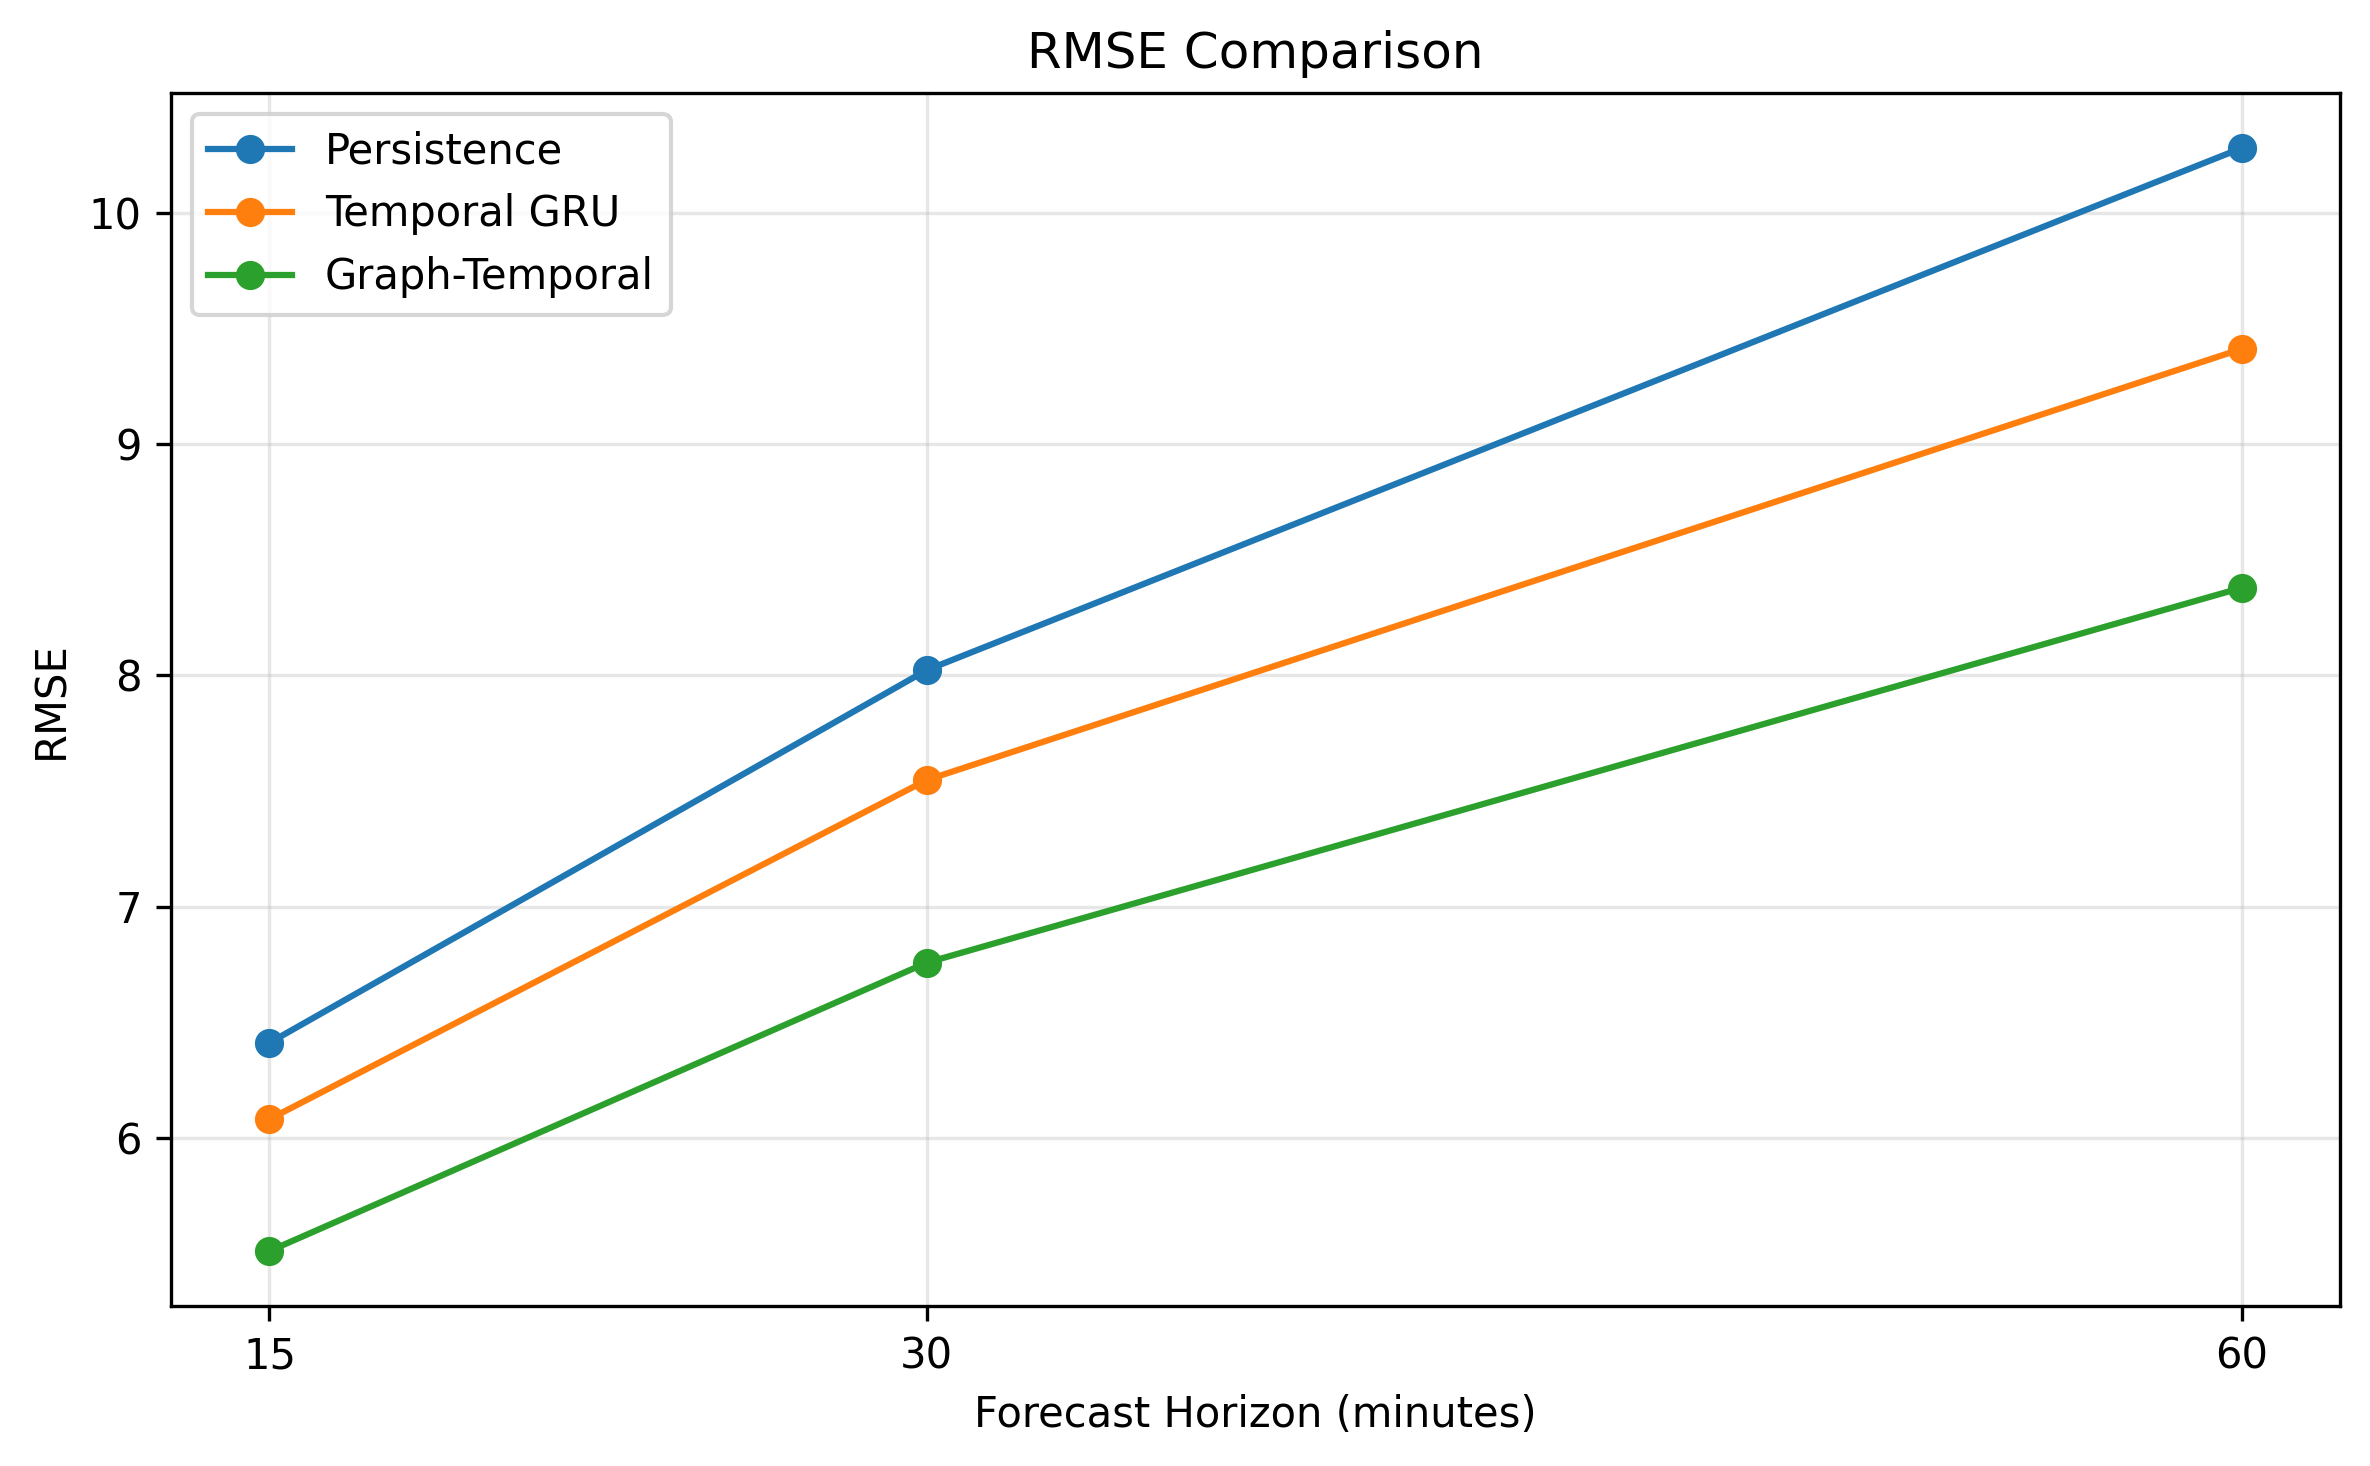
\includegraphics[width=\linewidth]{img/model_comparison/rmse_model_comparison}
    \end{minipage}

    \caption{Point forecasting performance of the Persistence, Temporal,
    and Graph-Temporal models across the three forecasting horizons in terms
    of MAE (left) and RMSE (right).}
    \label{fig:point_performance}
\end{figure}



\subsection{Probabilistic Forecasting and Calibration}
\label{subsec:probabilistic_results}

The probabilistic forecasting performance of the Temporal GRU and
Graph-Temporal models is reported in Table~\ref{tab:probabilistic_results}.
The Pinball Loss is evaluated separately for the three predicted quantiles,
while empirical coverage and interval width are used to assess the reliability
and sharpness of the nominal 80\% prediction intervals.

Across all forecasting horizons, the Graph-Temporal model achieves lower
Pinball Loss for each of the three quantiles. At 15 minutes, the losses for
$q_{0.1}$, $q_{0.5}$, and $q_{0.9}$ decrease from 0.952, 1.540, and 0.643
for the Temporal GRU to 0.845, 1.451, and 0.597 for the Graph-Temporal
model. The same behavior is observed at 30 and 60 minutes, indicating that
the benefit of incorporating spatial information is not limited to the
median forecast, but also extends to the estimation of the lower and upper
quantiles.

The two models, however, exhibit a different trade-off between calibration
and sharpness. The Temporal GRU achieves empirical coverage close to the
nominal 80\% level, with values of 81.30\%, 80.16\%, and 79.81\% at 15,
30, and 60 minutes, respectively. The Graph-Temporal model produces narrower
prediction intervals at every horizon, reducing the average interval width
from 9.339 to 8.929 at 15 minutes, from 10.931 to 10.485 at 30 minutes, and
from 13.309 to 12.470 at 60 minutes. This increased sharpness is accompanied
by slightly lower coverage, which remains between 78.13\% and 78.44\% across
the three horizons.

These results show that the Graph-Temporal model improves the quality of all
three estimated quantiles and produces more concentrated predictive
intervals, but the resulting intervals exhibit mild undercoverage relative
to the nominal 80\% level. In contrast, the Temporal GRU remains closer to
the nominal coverage overall, although it exhibits mild overcoverage at the
15-minute horizon, reaching 81.30\%.
The reliability--sharpness trade-off is further illustrated in
Figure~\ref{fig:probabilistic_comparison}.
Moreover, interval width increases with the
forecasting horizon for both models, reflecting the greater uncertainty of
longer-term predictions. The calibration behavior of the selected
Graph-Temporal model is further investigated under distribution shift in
Section~\ref{sec:distribution_shift}.

\begin{table}[t]
    \centering
    \caption{Probabilistic forecasting performance on the test set. Coverage
    refers to the nominal 80\% prediction interval defined by
    $q_{0.1}$ and $q_{0.9}$.}
    \label{tab:probabilistic_results}
    \resizebox{\linewidth}{!}{
    \begin{tabular}{llccccc}
        \toprule
        Model & Horizon
        & Pinball $q_{0.1}$
        & Pinball $q_{0.5}$
        & Pinball $q_{0.9}$
        & Coverage (\%)
        & Interval Width \\
        \midrule

        Temporal GRU
        & 15 min & 0.952 & 1.540 & 0.643 & 81.30 & 9.339 \\
        & 30 min & 1.225 & 1.867 & 0.743 & 80.16 & 10.931 \\
        & 60 min & 1.668 & 2.367 & 0.832 & 79.81 & 13.309 \\
        \midrule

        Graph-Temporal
        & 15 min & \textbf{0.845} & \textbf{1.451} & \textbf{0.597}
        & 78.44 & \textbf{8.929} \\
        & 30 min & \textbf{1.028} & \textbf{1.721} & \textbf{0.677}
        & 78.22 & \textbf{10.485} \\
        & 60 min & \textbf{1.320} & \textbf{2.122} & \textbf{0.775}
        & 78.13 & \textbf{12.470} \\
        \bottomrule
    \end{tabular}
    }
\end{table}

\begin{figure}[t]
    \centering

    \begin{minipage}[b]{0.49\linewidth}
        \centering
        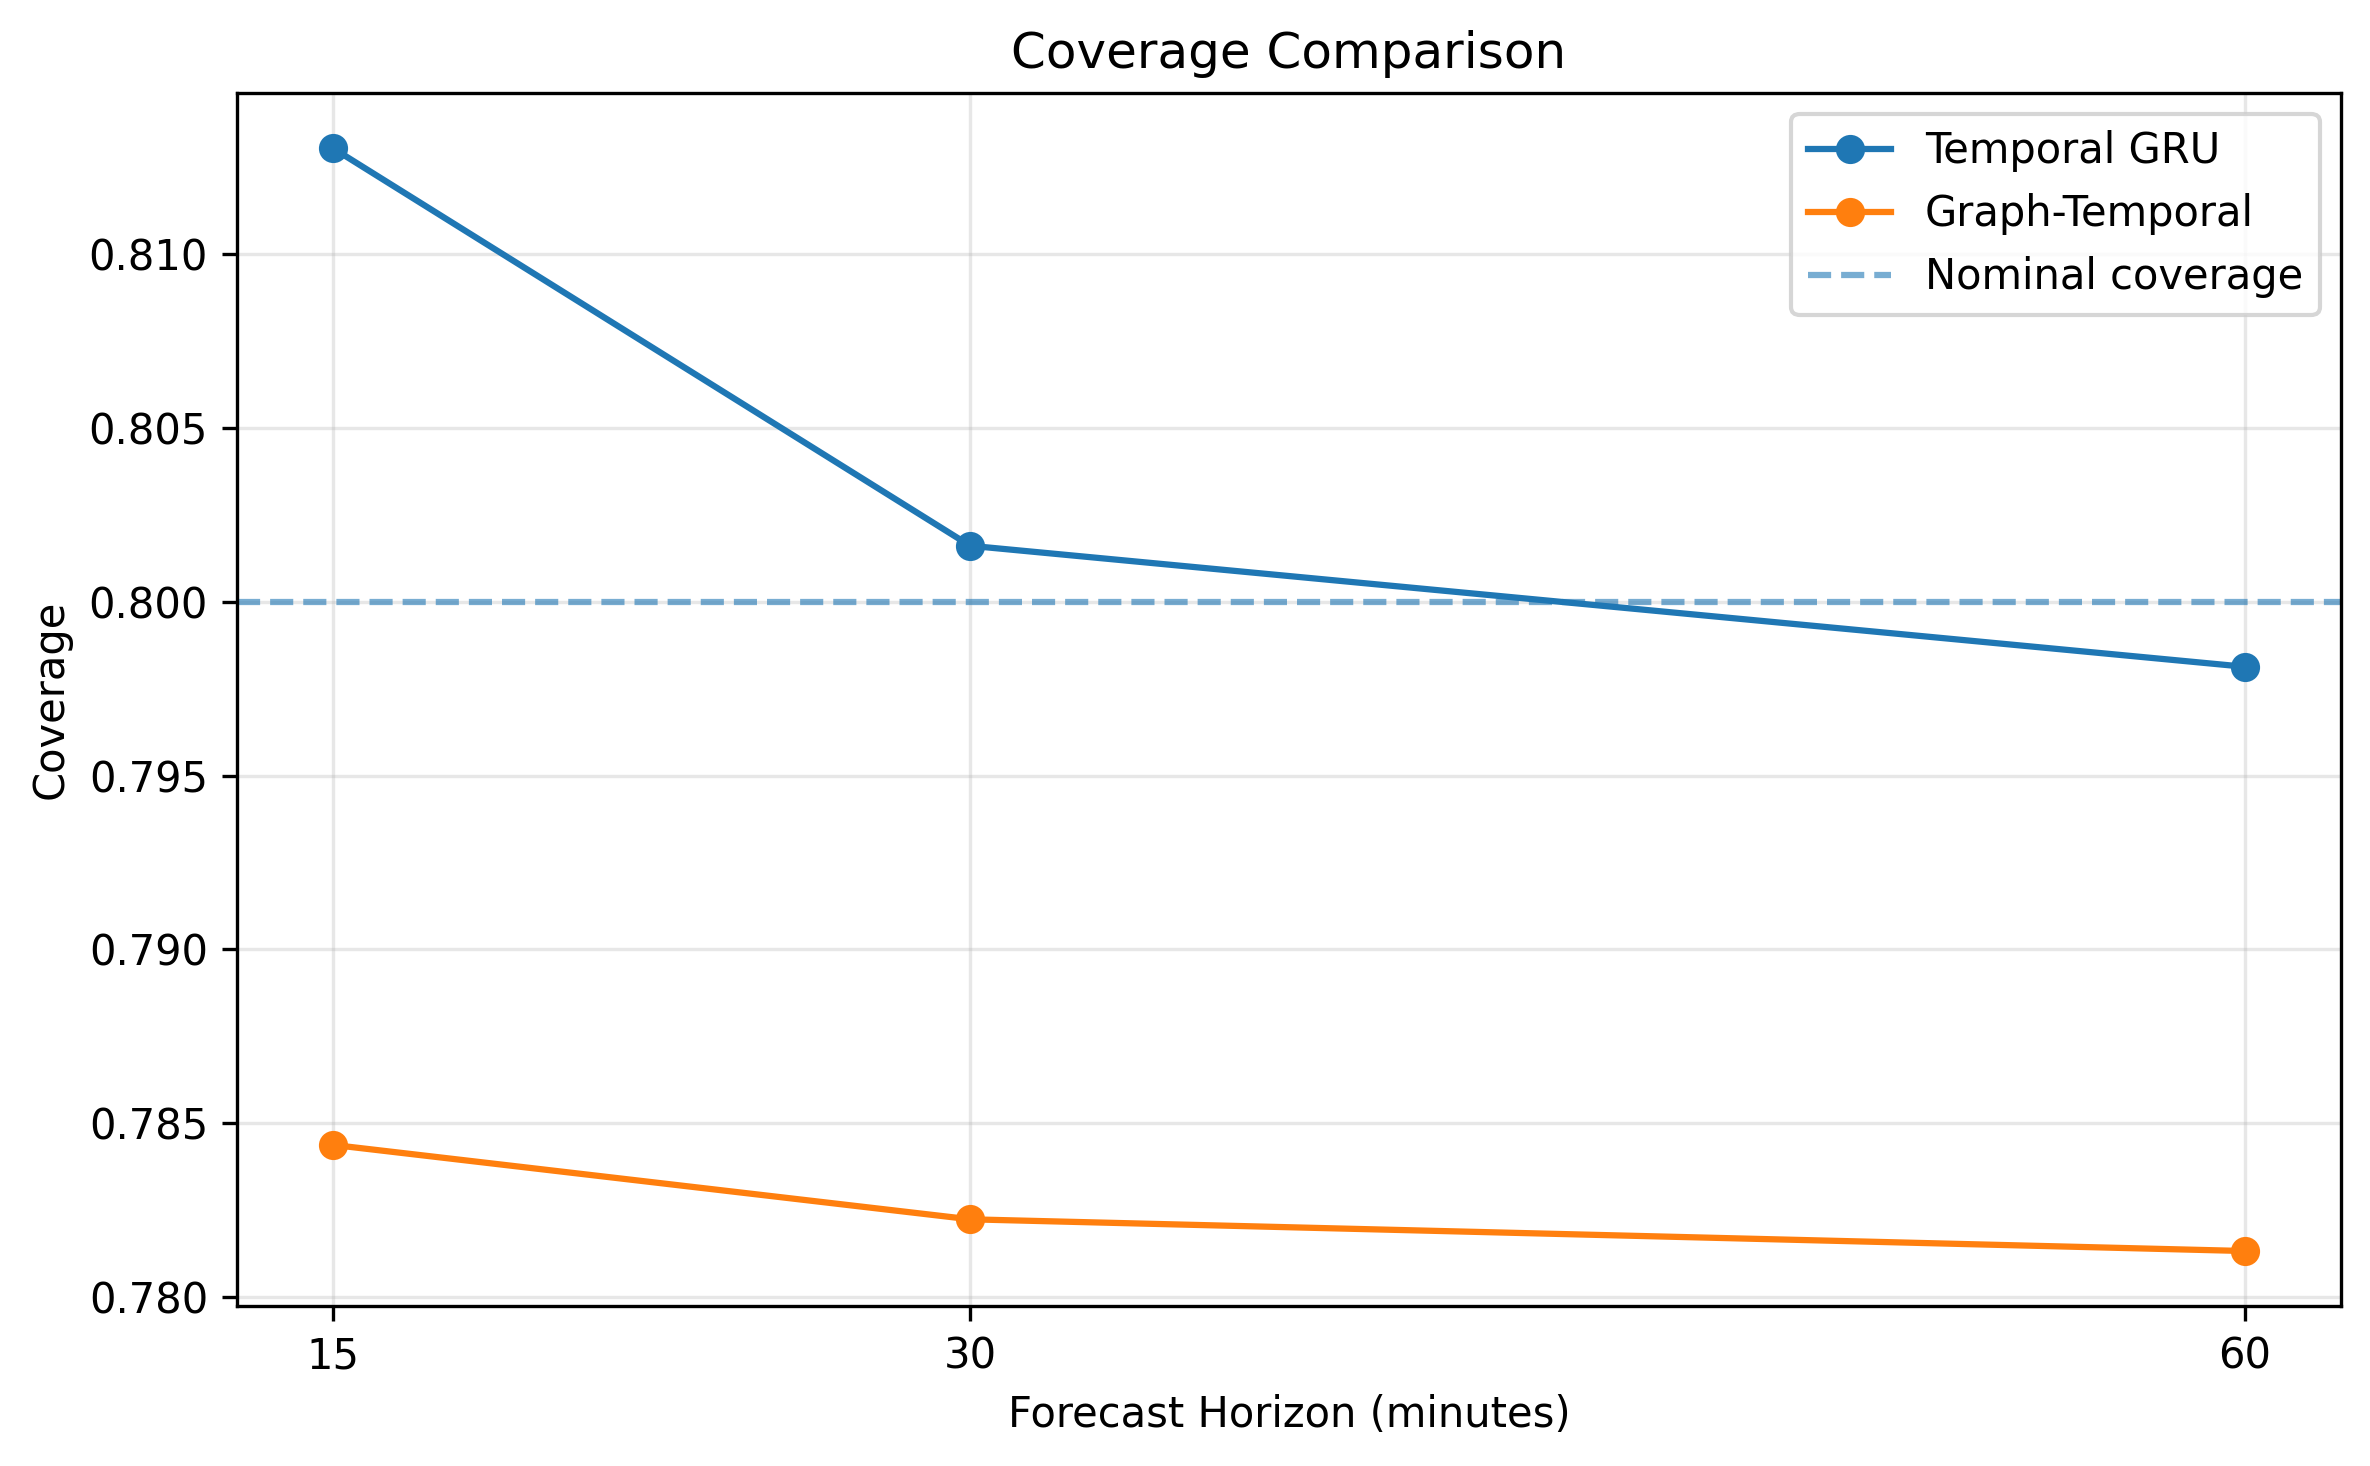
\includegraphics[width=\linewidth]{img/model_comparison/coverage_model_comparison}
    \end{minipage}
    \hfill
    \begin{minipage}[b]{0.49\linewidth}
        \centering
        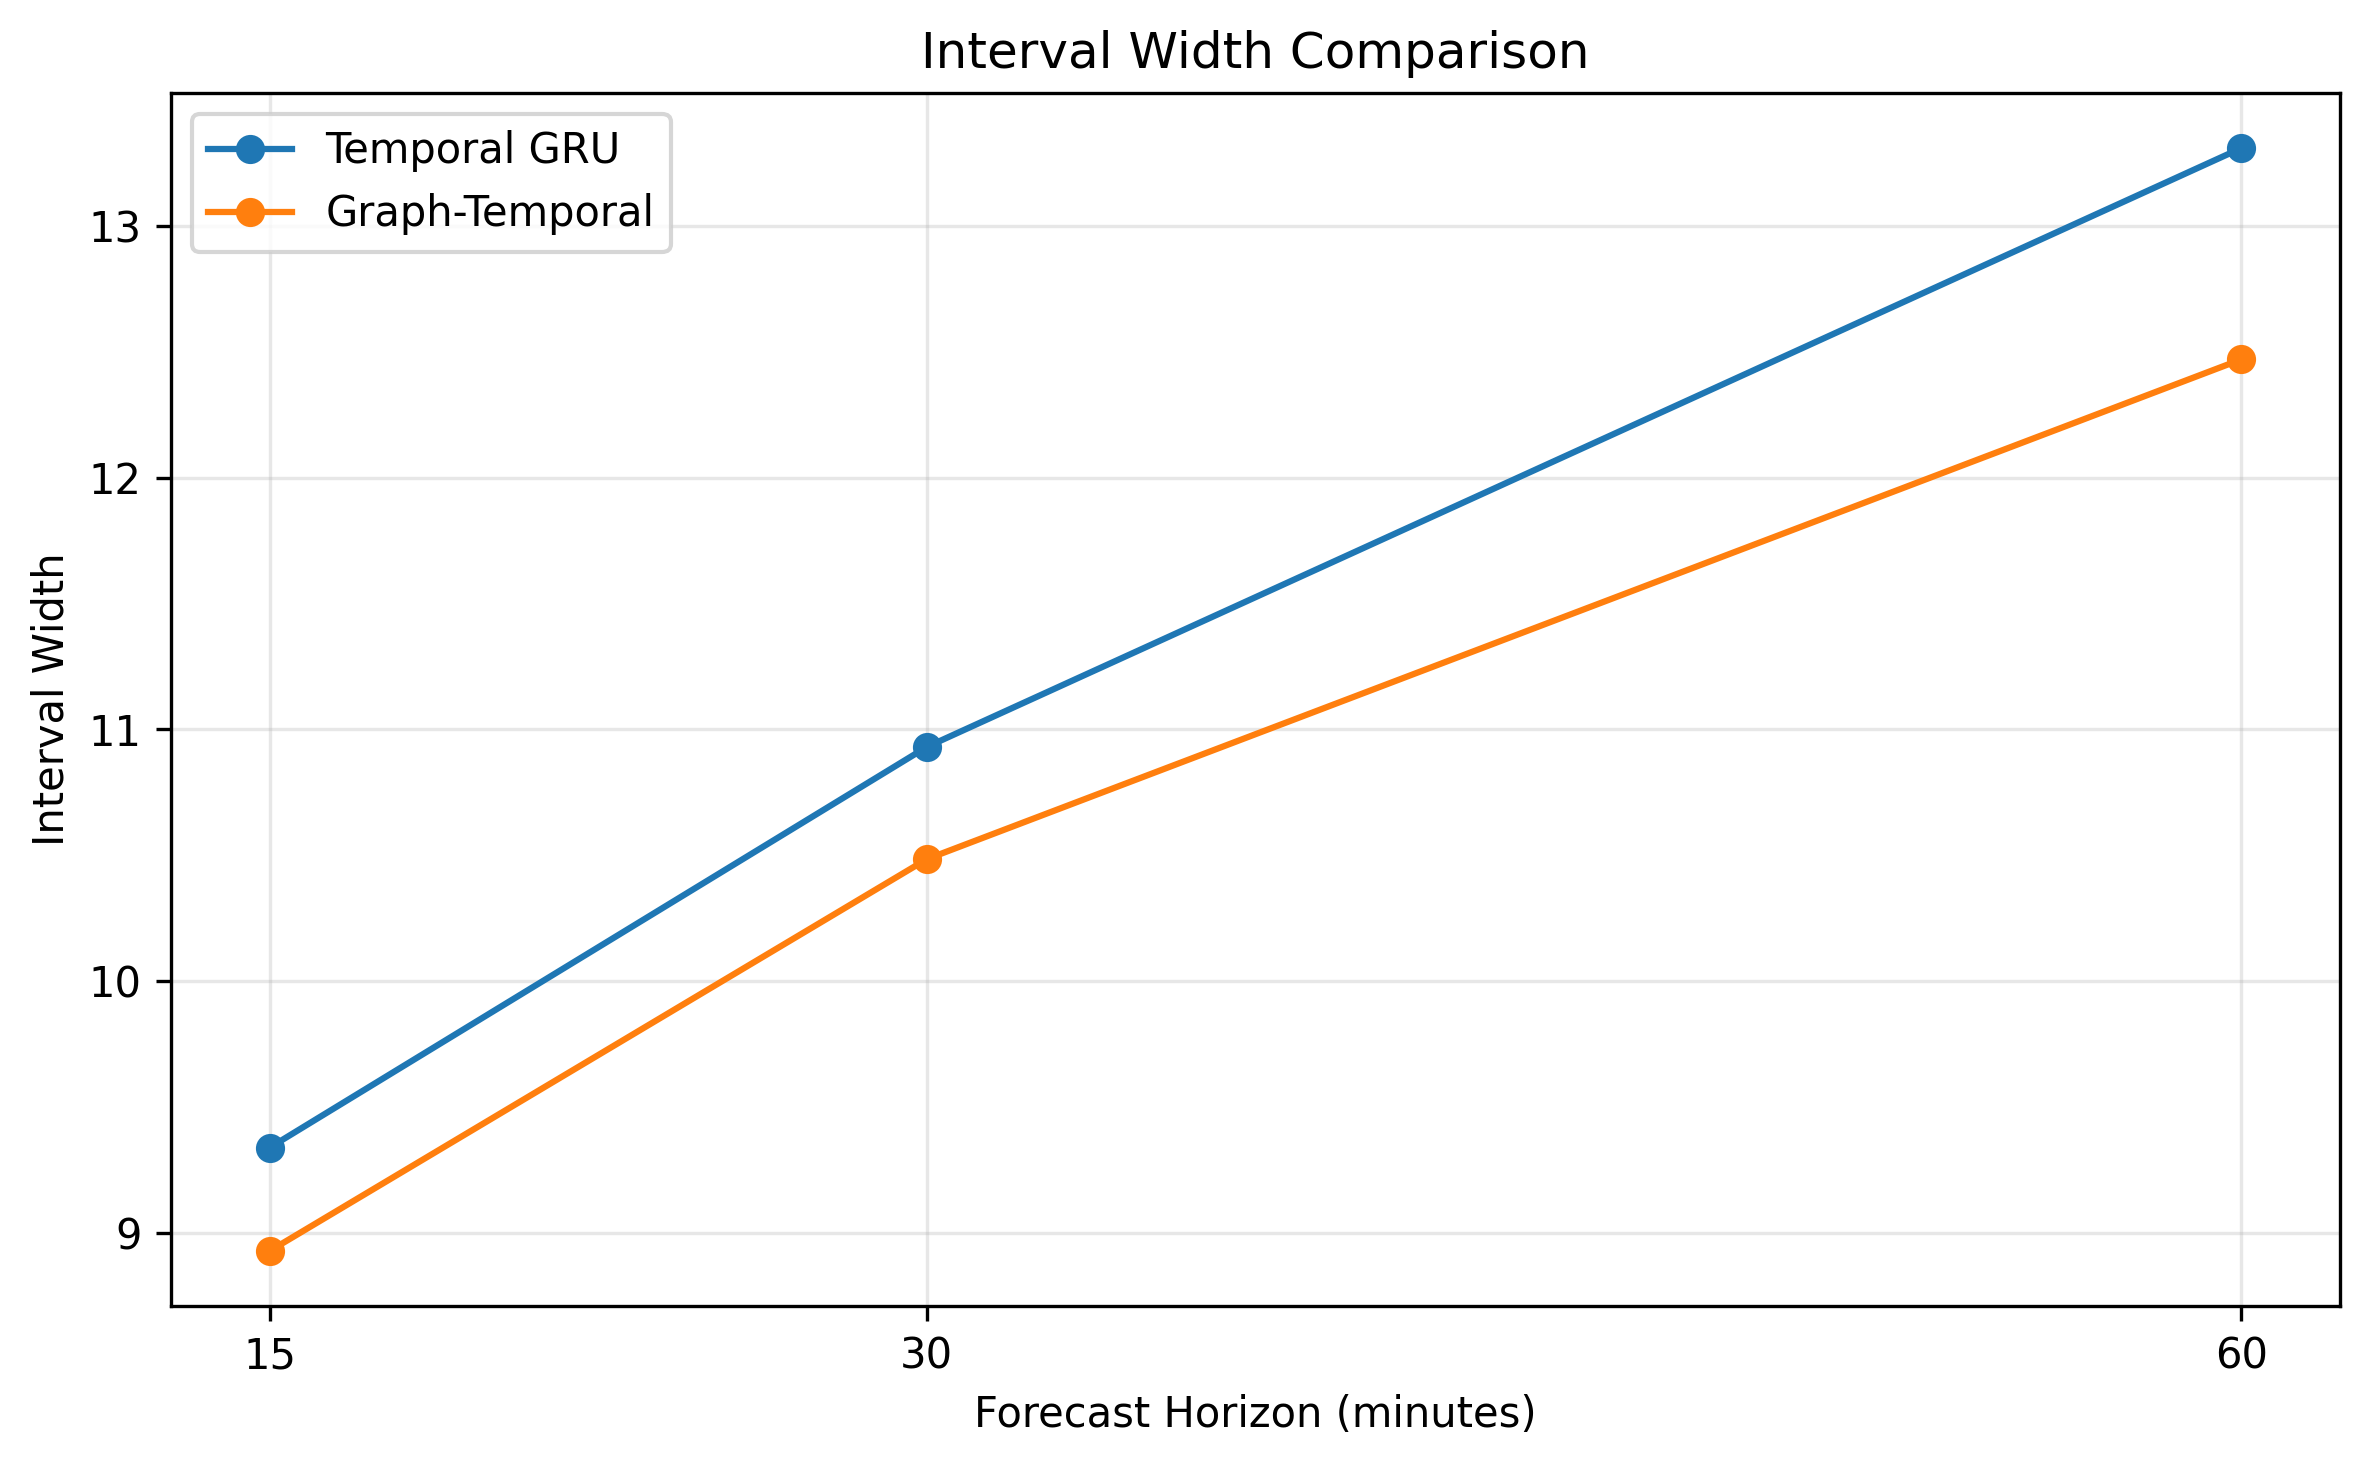
\includegraphics[width=\linewidth]{img/model_comparison/interval_width_model_comparison}
    \end{minipage}

    \caption{Comparison of the probabilistic forecasts produced by the
    Temporal GRU and Graph-Temporal models in terms of empirical coverage
    (left) and prediction interval width (right) across the three forecasting
    horizons. The dashed line in the coverage plot represents the nominal
    80\% coverage level.}
    \label{fig:probabilistic_comparison}
\end{figure}

Quantile crossing is negligible for both models, with rates below 0.05\%
at every forecasting horizon, indicating that the predicted quantiles
almost always preserve their expected ordering.

A more detailed view of probabilistic reliability is provided by the
calibration curves in Figure~\ref{fig:quantile_calibration}. The plots compare the
nominal quantile levels with their empirical frequencies and complement the
interval-level coverage results reported in
Table~\ref{tab:probabilistic_results}.

\begin{figure}[t]
    \centering

    \begin{minipage}[b]{0.49\linewidth}
        \centering
        
\includegraphics[width=\linewidth]{img/temporal_gru/calibration_plot}
    \end{minipage}
    \hfill
    \begin{minipage}[b]{0.49\linewidth}
        \centering
        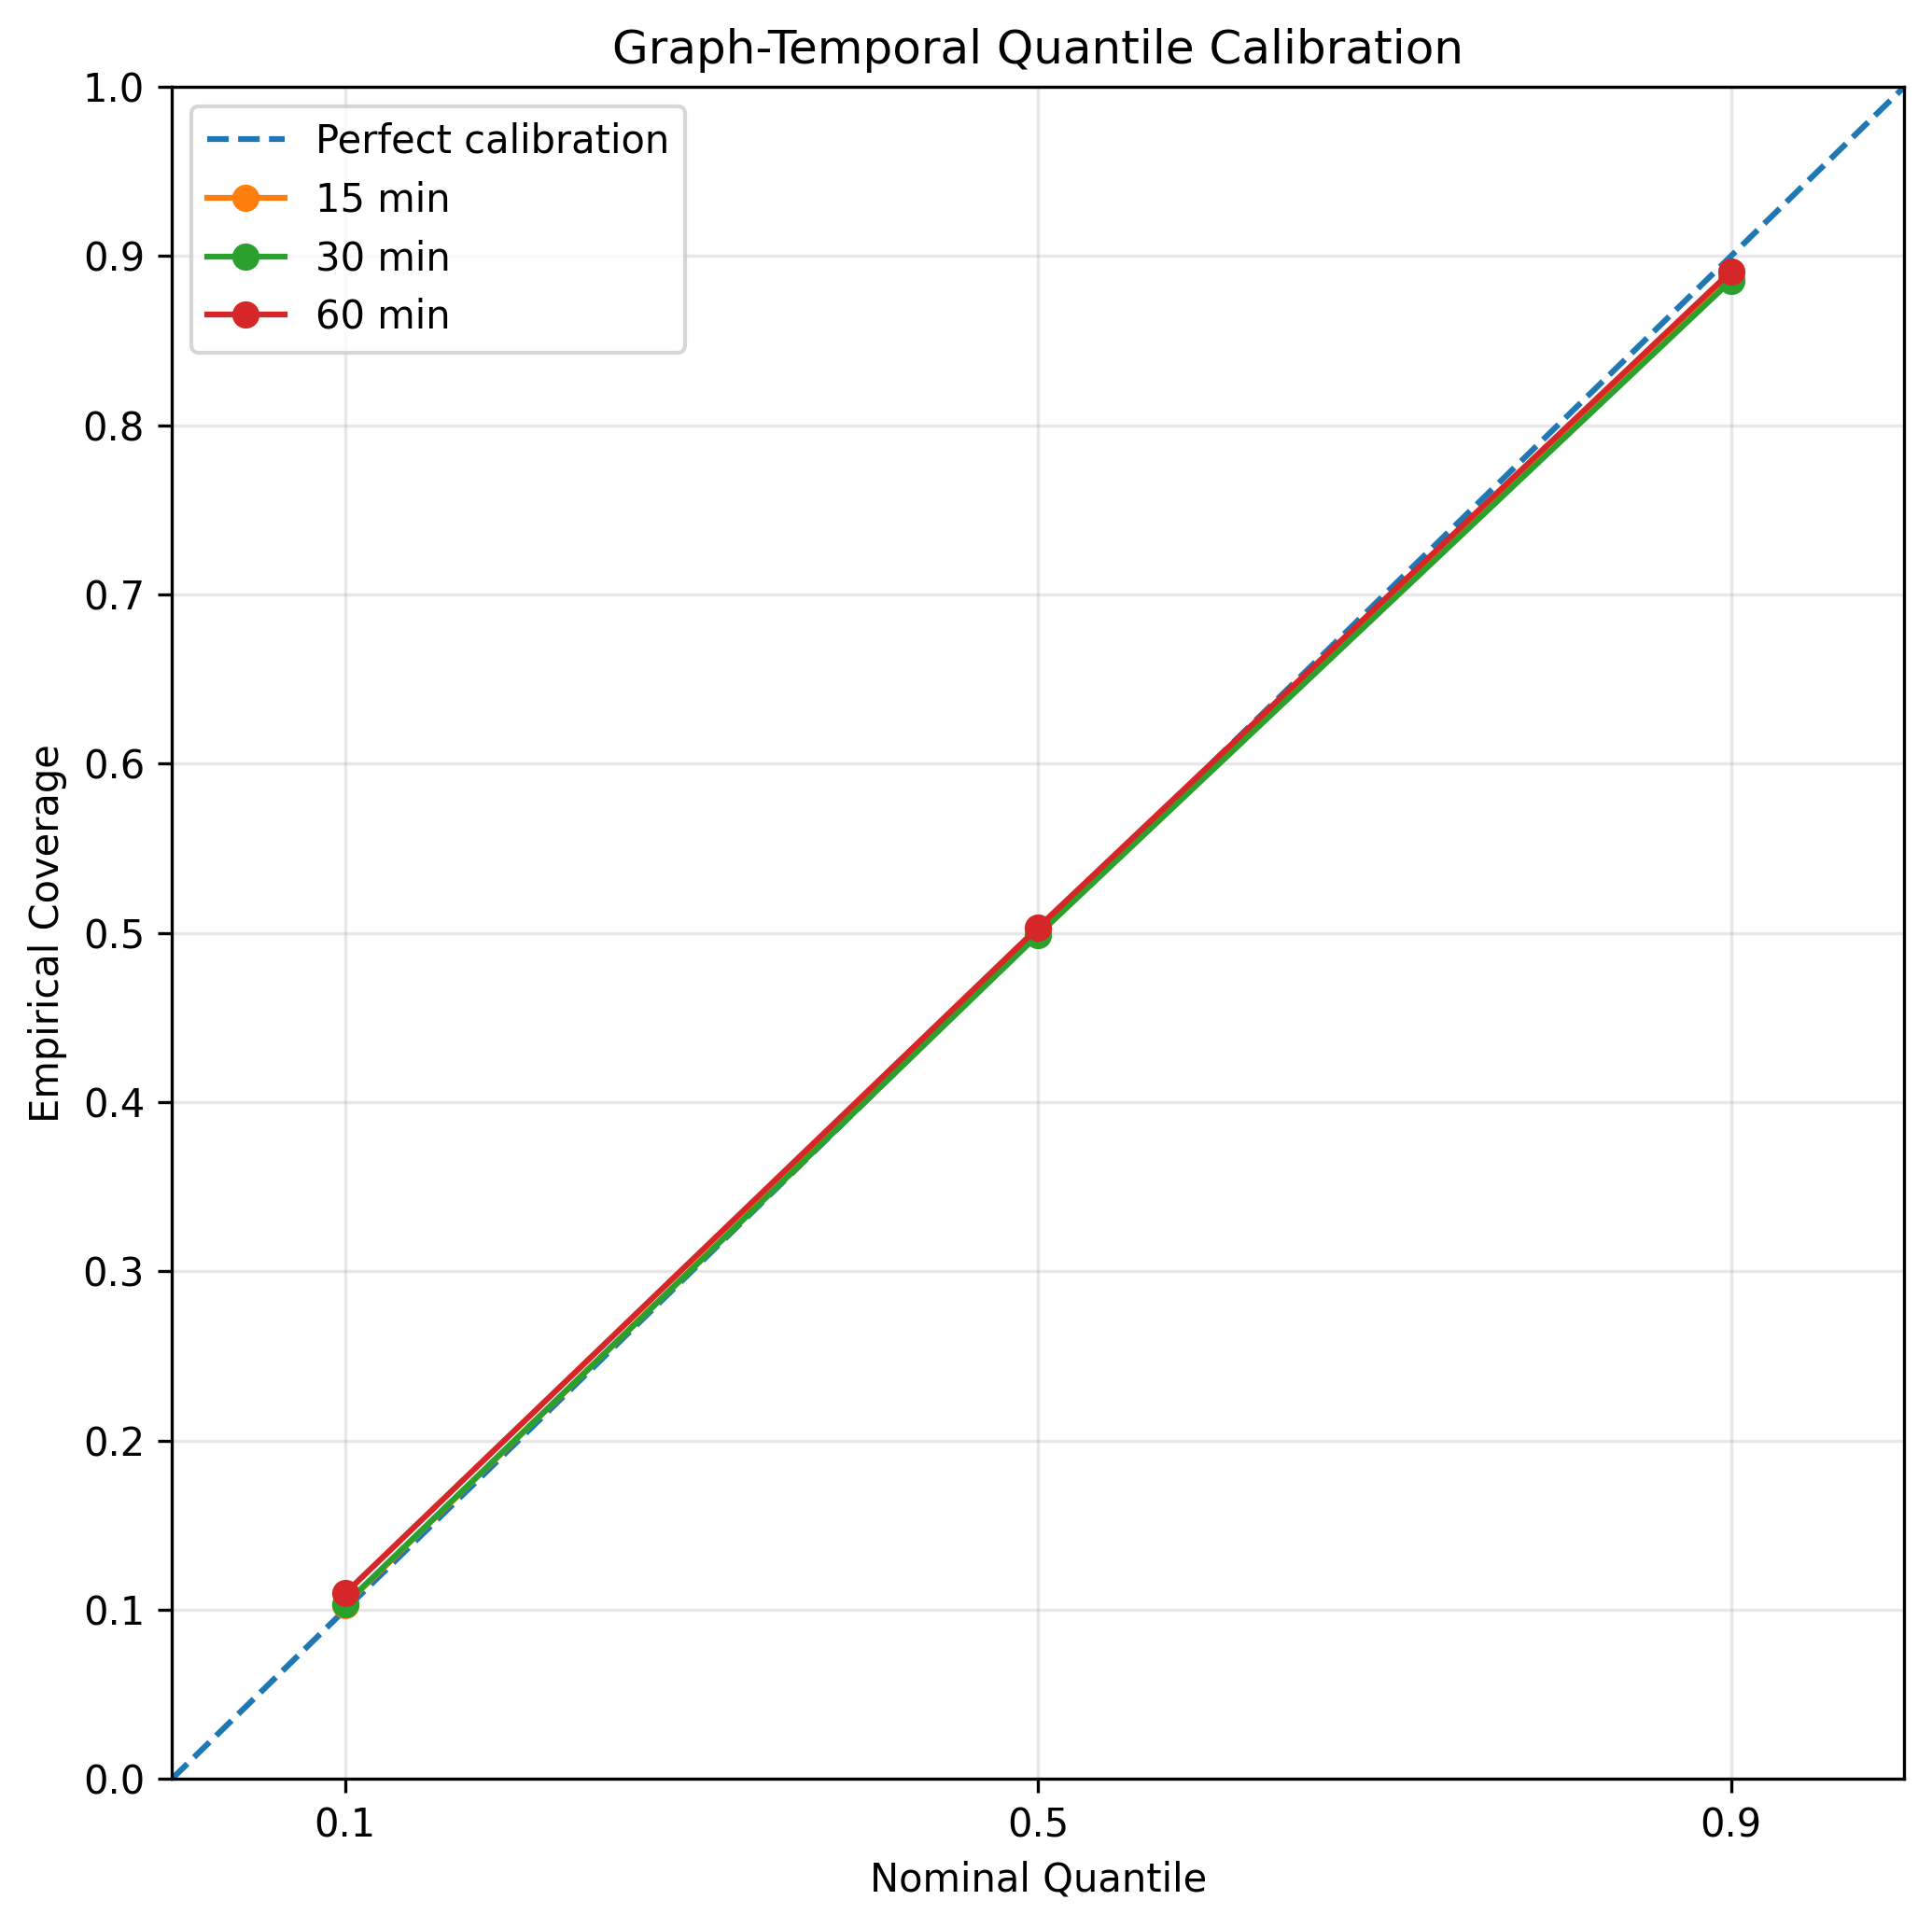
\includegraphics[width=\linewidth]{img/graph_temporal/calibration_plot}
    \end{minipage}

    \caption{Quantile calibration of the Temporal (left) and
    Graph-Temporal (right) models at the three forecasting horizons.
    The dashed diagonal represents perfect calibration.}
    \label{fig:quantile_calibration}
\end{figure}
%\section{Analysis of the Graph Component}
\label{sec:graph_analysis}

\subsection{When Does the Graph Help?}
\label{subsec:graph_effect}

The aggregate results presented in Section~\ref{sec:in_distribution_results}
show that incorporating graph information improves forecasting accuracy at
all three horizons. To determine whether this improvement is widespread
across the road network or concentrated on a limited subset of sensors, the
two neural models were additionally compared at sensor level.

For each sensor $n$ and forecasting horizon $h$, the effect of graph message
passing is quantified as the difference between the MAE of the Temporal
and that of the Graph-Temporal model,

\begin{equation}
    \Delta \mathrm{MAE}_{n,h}
    =
    \mathrm{MAE}^{\mathrm{Temporal}}_{n,h}
    -
    \mathrm{MAE}^{\mathrm{Graph}}_{n,h}.
    \label{eq:delta_mae}
\end{equation}

A positive value of $\Delta \mathrm{MAE}_{n,h}$ therefore indicates that
incorporating graph information reduces the forecasting error for sensor
$n$, whereas a negative value indicates that the Temporal GRU performs
better for that sensor.

The sensor-level comparison shows that the aggregate improvement is not
driven by only a small subset of locations. The Graph-Temporal model reduces
MAE for 199 out of 207 sensors at the 15-minute horizon and for 200 out of
207 sensors at 30 minutes. At 60 minutes, graph message passing remains
beneficial for 193 out of 207 sensors. Therefore, the advantage observed in
the aggregate metrics is distributed across the large majority of the sensor
network, although a small number of locations consistently or occasionally
benefit more from purely temporal modeling.

To complement the sensor-level aggregate analysis, representative forecasting
examples are examined in Figure~\ref{fig:graph_help_examples}. The examples
compare the predictions of the Temporal GRU and Graph-Temporal model for
sensor-time pairs in which the inclusion of spatial information produces a
clear reduction in forecasting error.

\begin{figure}[t]
    \centering

    \begin{minipage}[b]{0.8\linewidth}
        \centering
        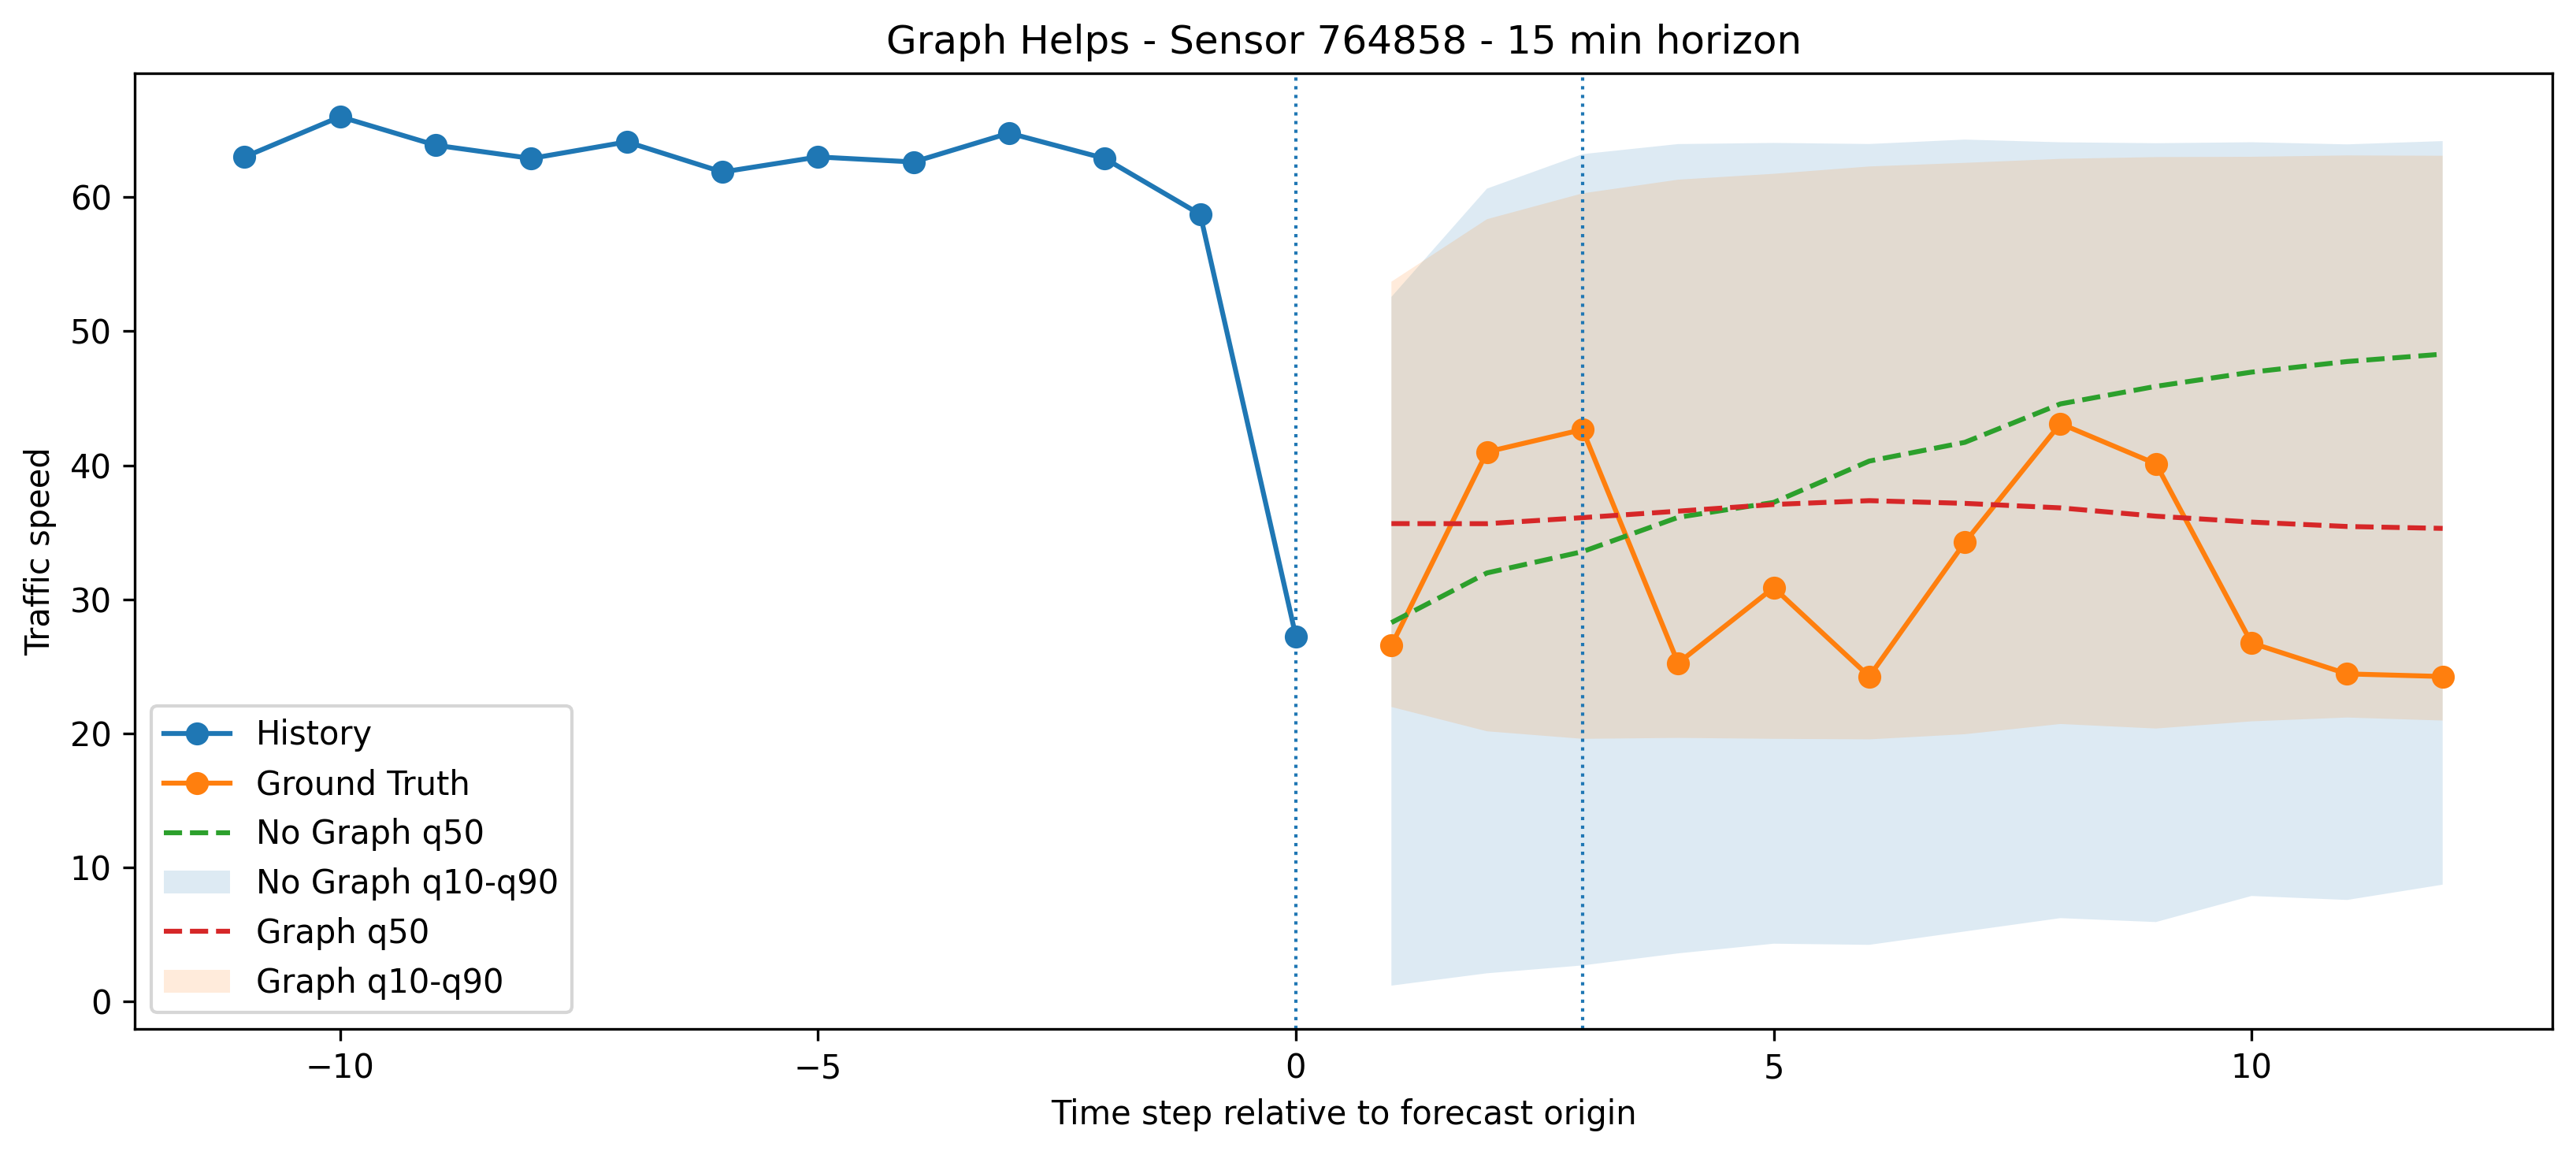
\includegraphics[width=\linewidth]{img/graph_impact_analysis/graph_helps_h3_sensor_764858}
    \end{minipage}
    \hfill
    \begin{minipage}[b]{0.8\linewidth}
        \centering
        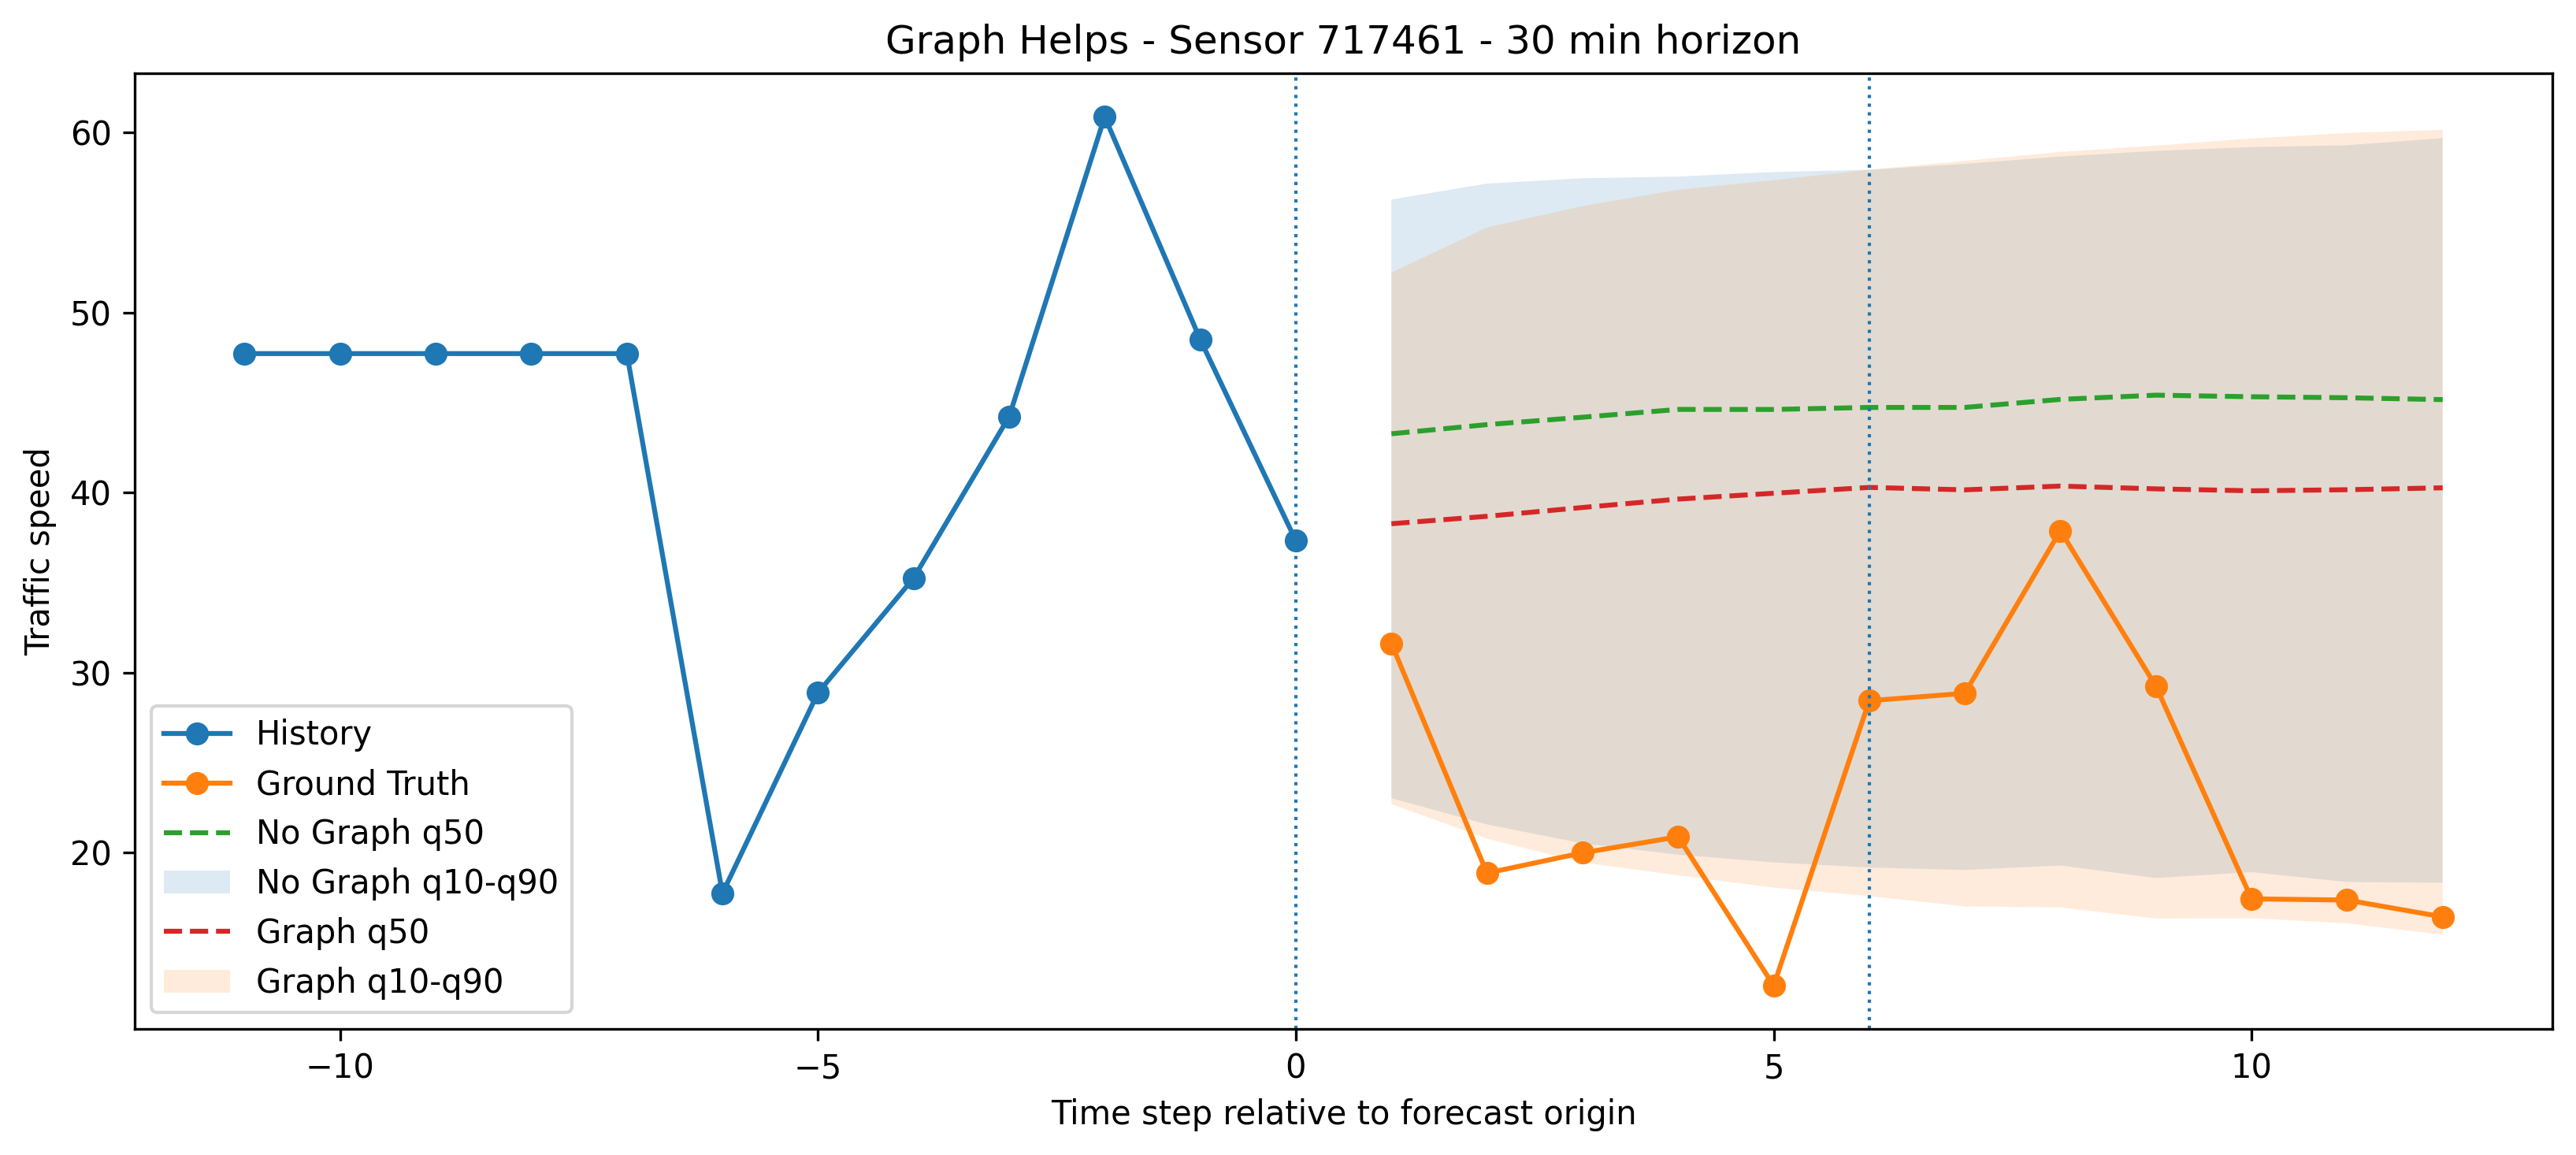
\includegraphics[width=\linewidth]{img/graph_impact_analysis/graph_helps_h6_sensor_717461}
    \end{minipage}
    \hfill
    \begin{minipage}[b]{0.8\linewidth}
        \centering
        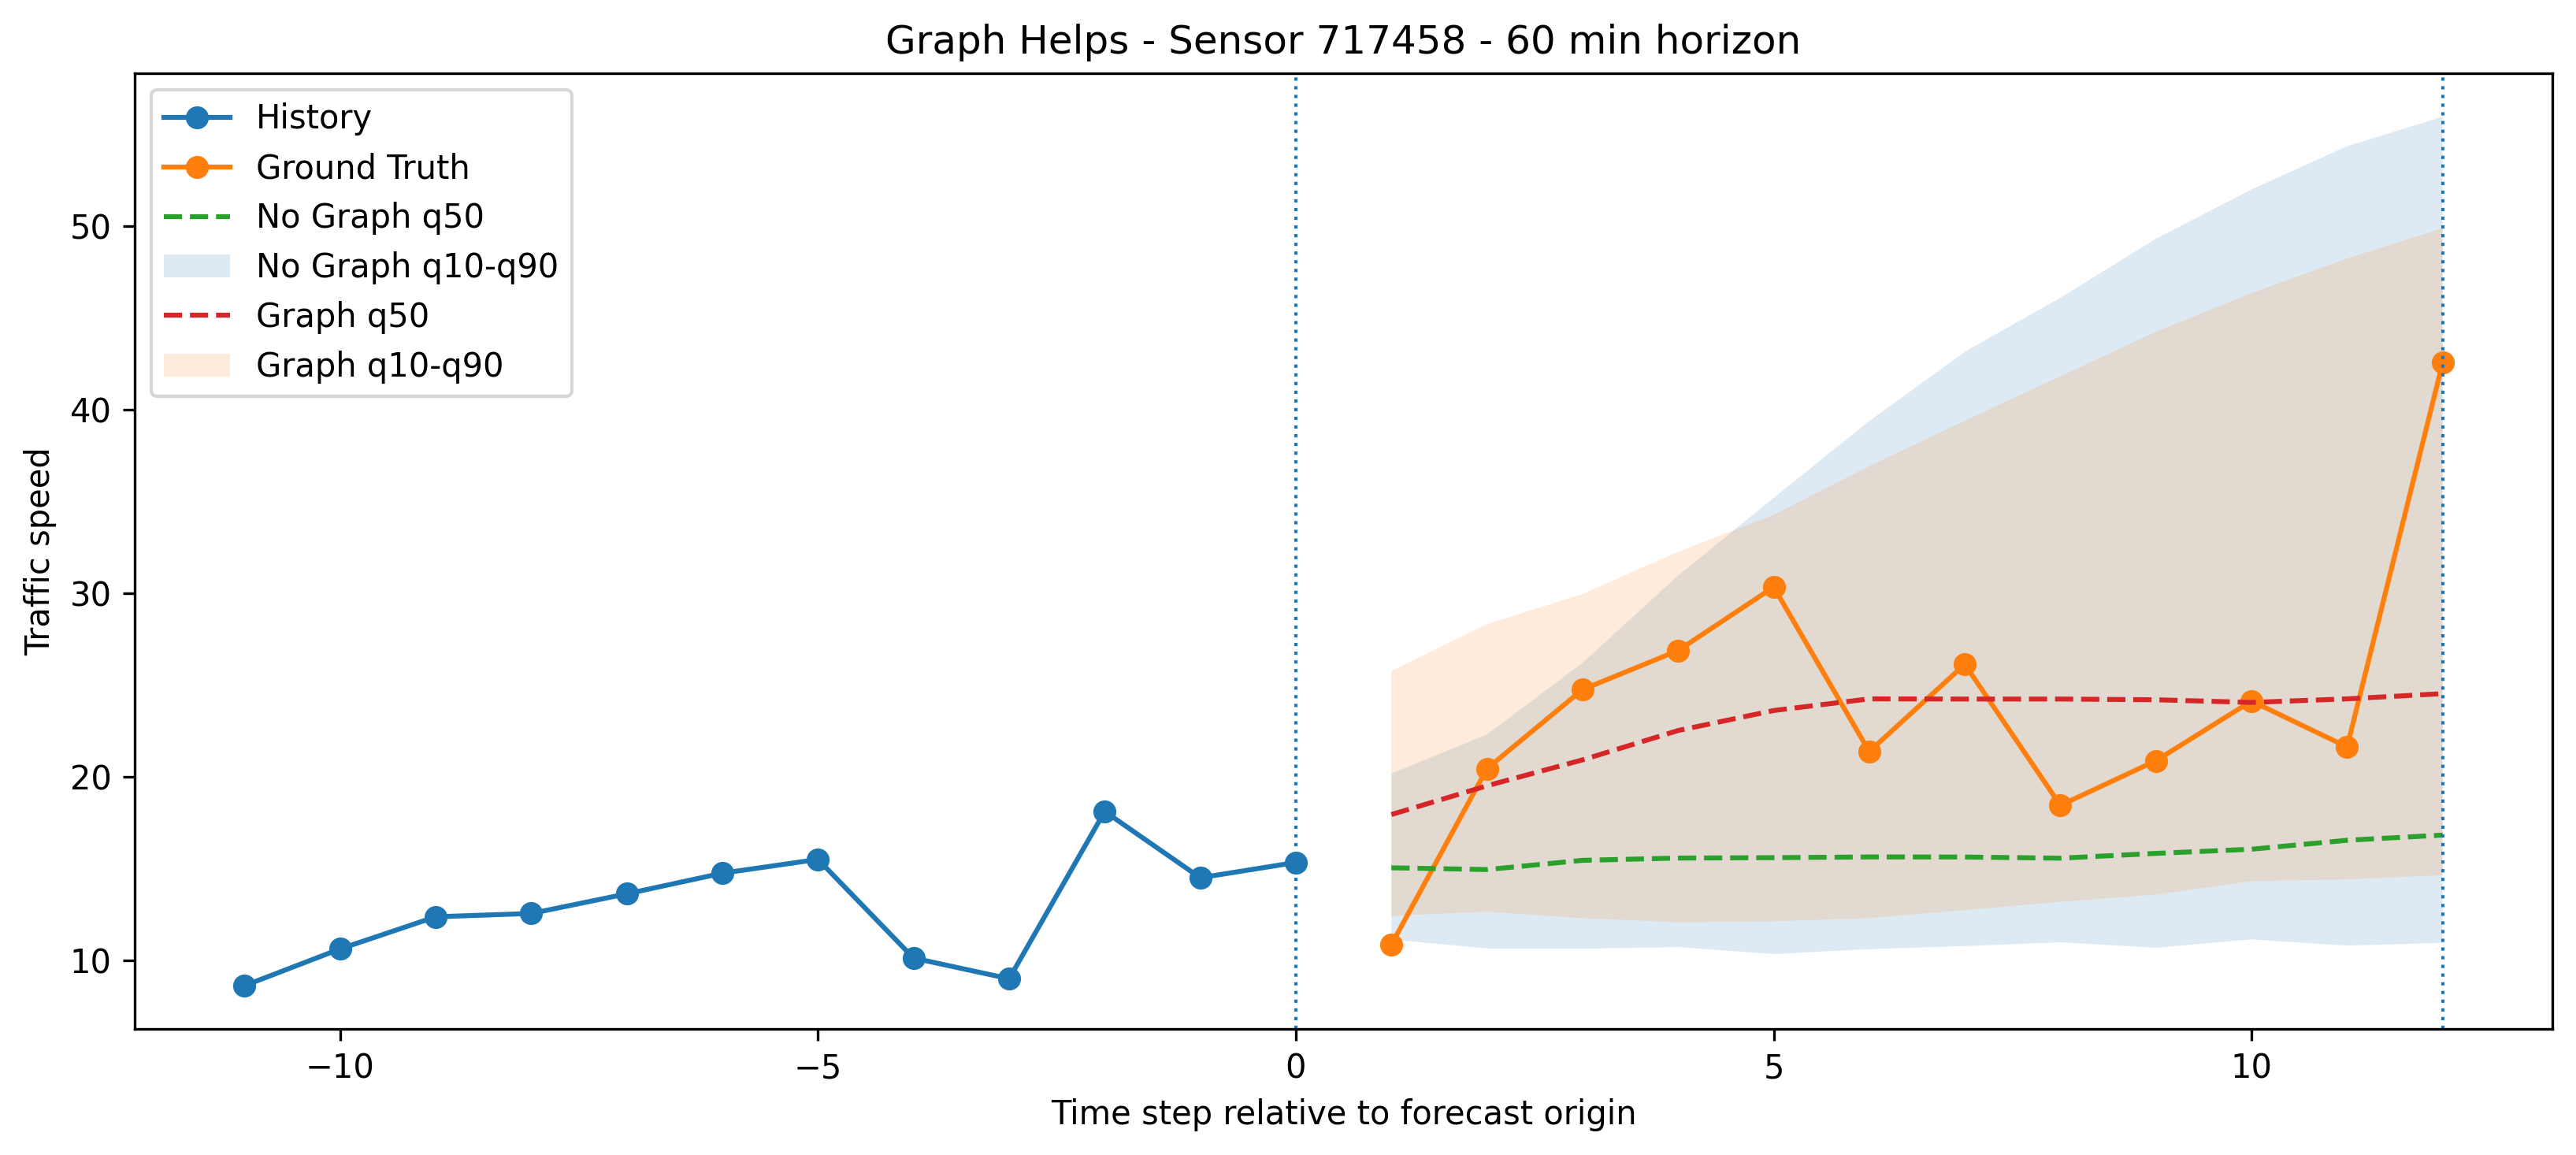
\includegraphics[width=\linewidth]{img/graph_impact_analysis/graph_helps_h12_sensor_717458}
    \end{minipage}

    \caption{Representative forecasting examples in which the Graph-Temporal
    model improves over the Temporal GRU at the 15-minute (left), 30-minute
    (center), and 60-minute (right) forecasting horizons.}
    \label{fig:graph_help_examples}
\end{figure}


Figure~\ref{fig:graph_hurt_examples} instead reports representative cases in
which graph message passing increases the forecasting error. These examples
are particularly useful because they show that neighboring information is
not always informative for the future evolution of a given sensor. The
presence of such cases motivates a more detailed investigation of whether the
benefit of graph message passing can be related to the local graph structure.

\begin{figure}[t]
    \centering

    \begin{minipage}[b]{0.8\linewidth}
        \centering
        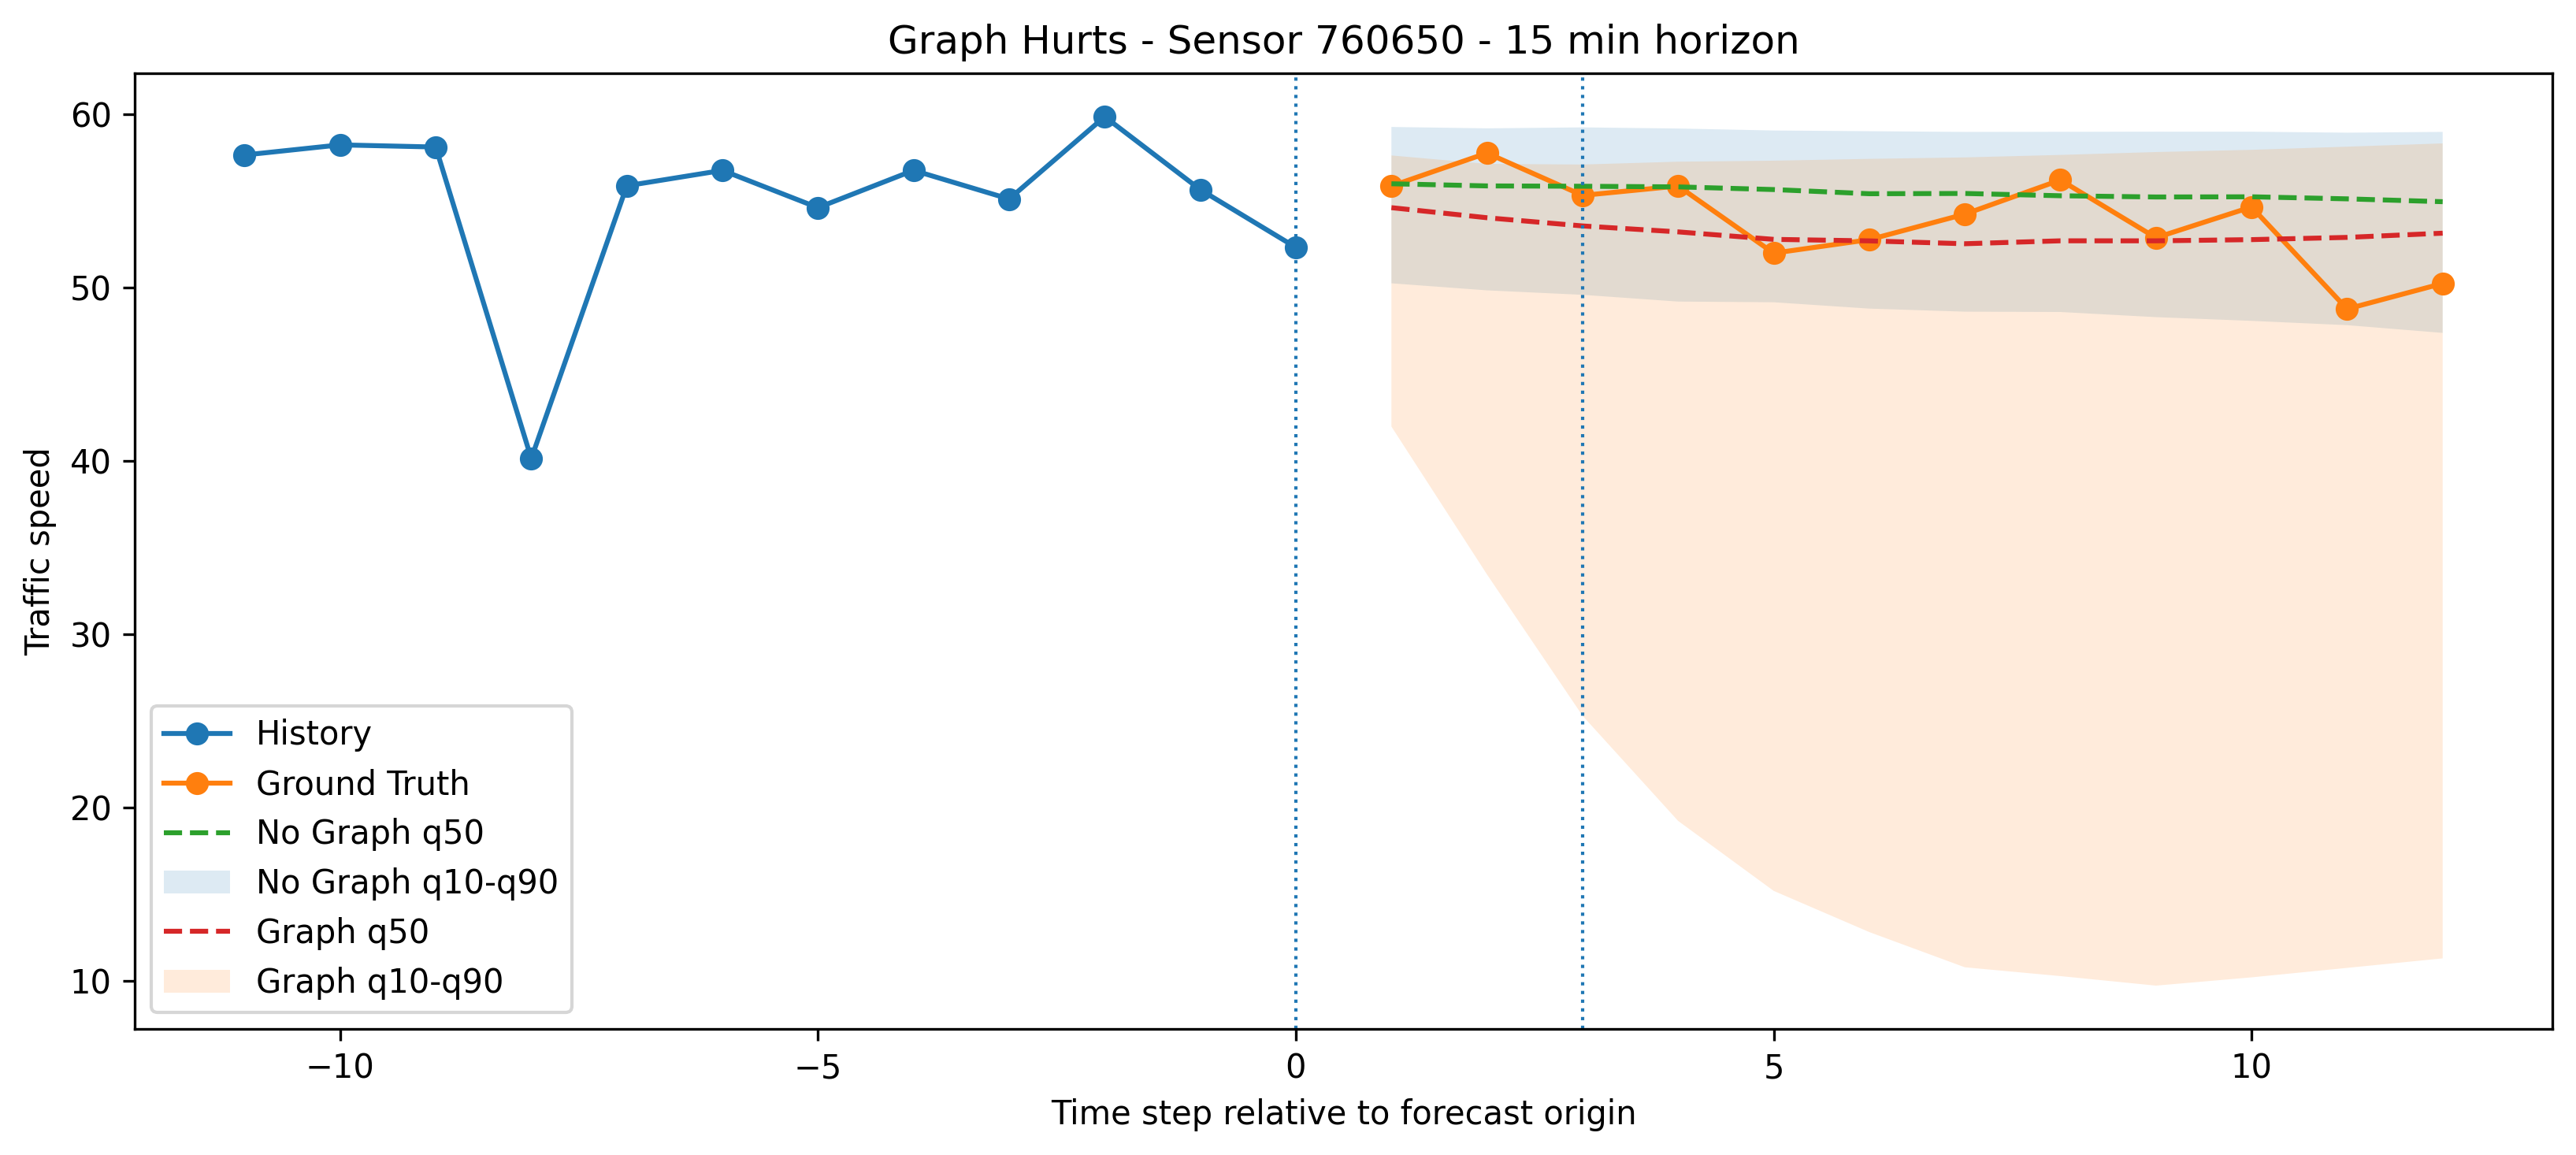
\includegraphics[width=\linewidth]{img/graph_impact_analysis/graph_hurts_h3_sensor_760650}
    \end{minipage}
    \hfill
    \begin{minipage}[b]{0.8\linewidth}
        \centering
        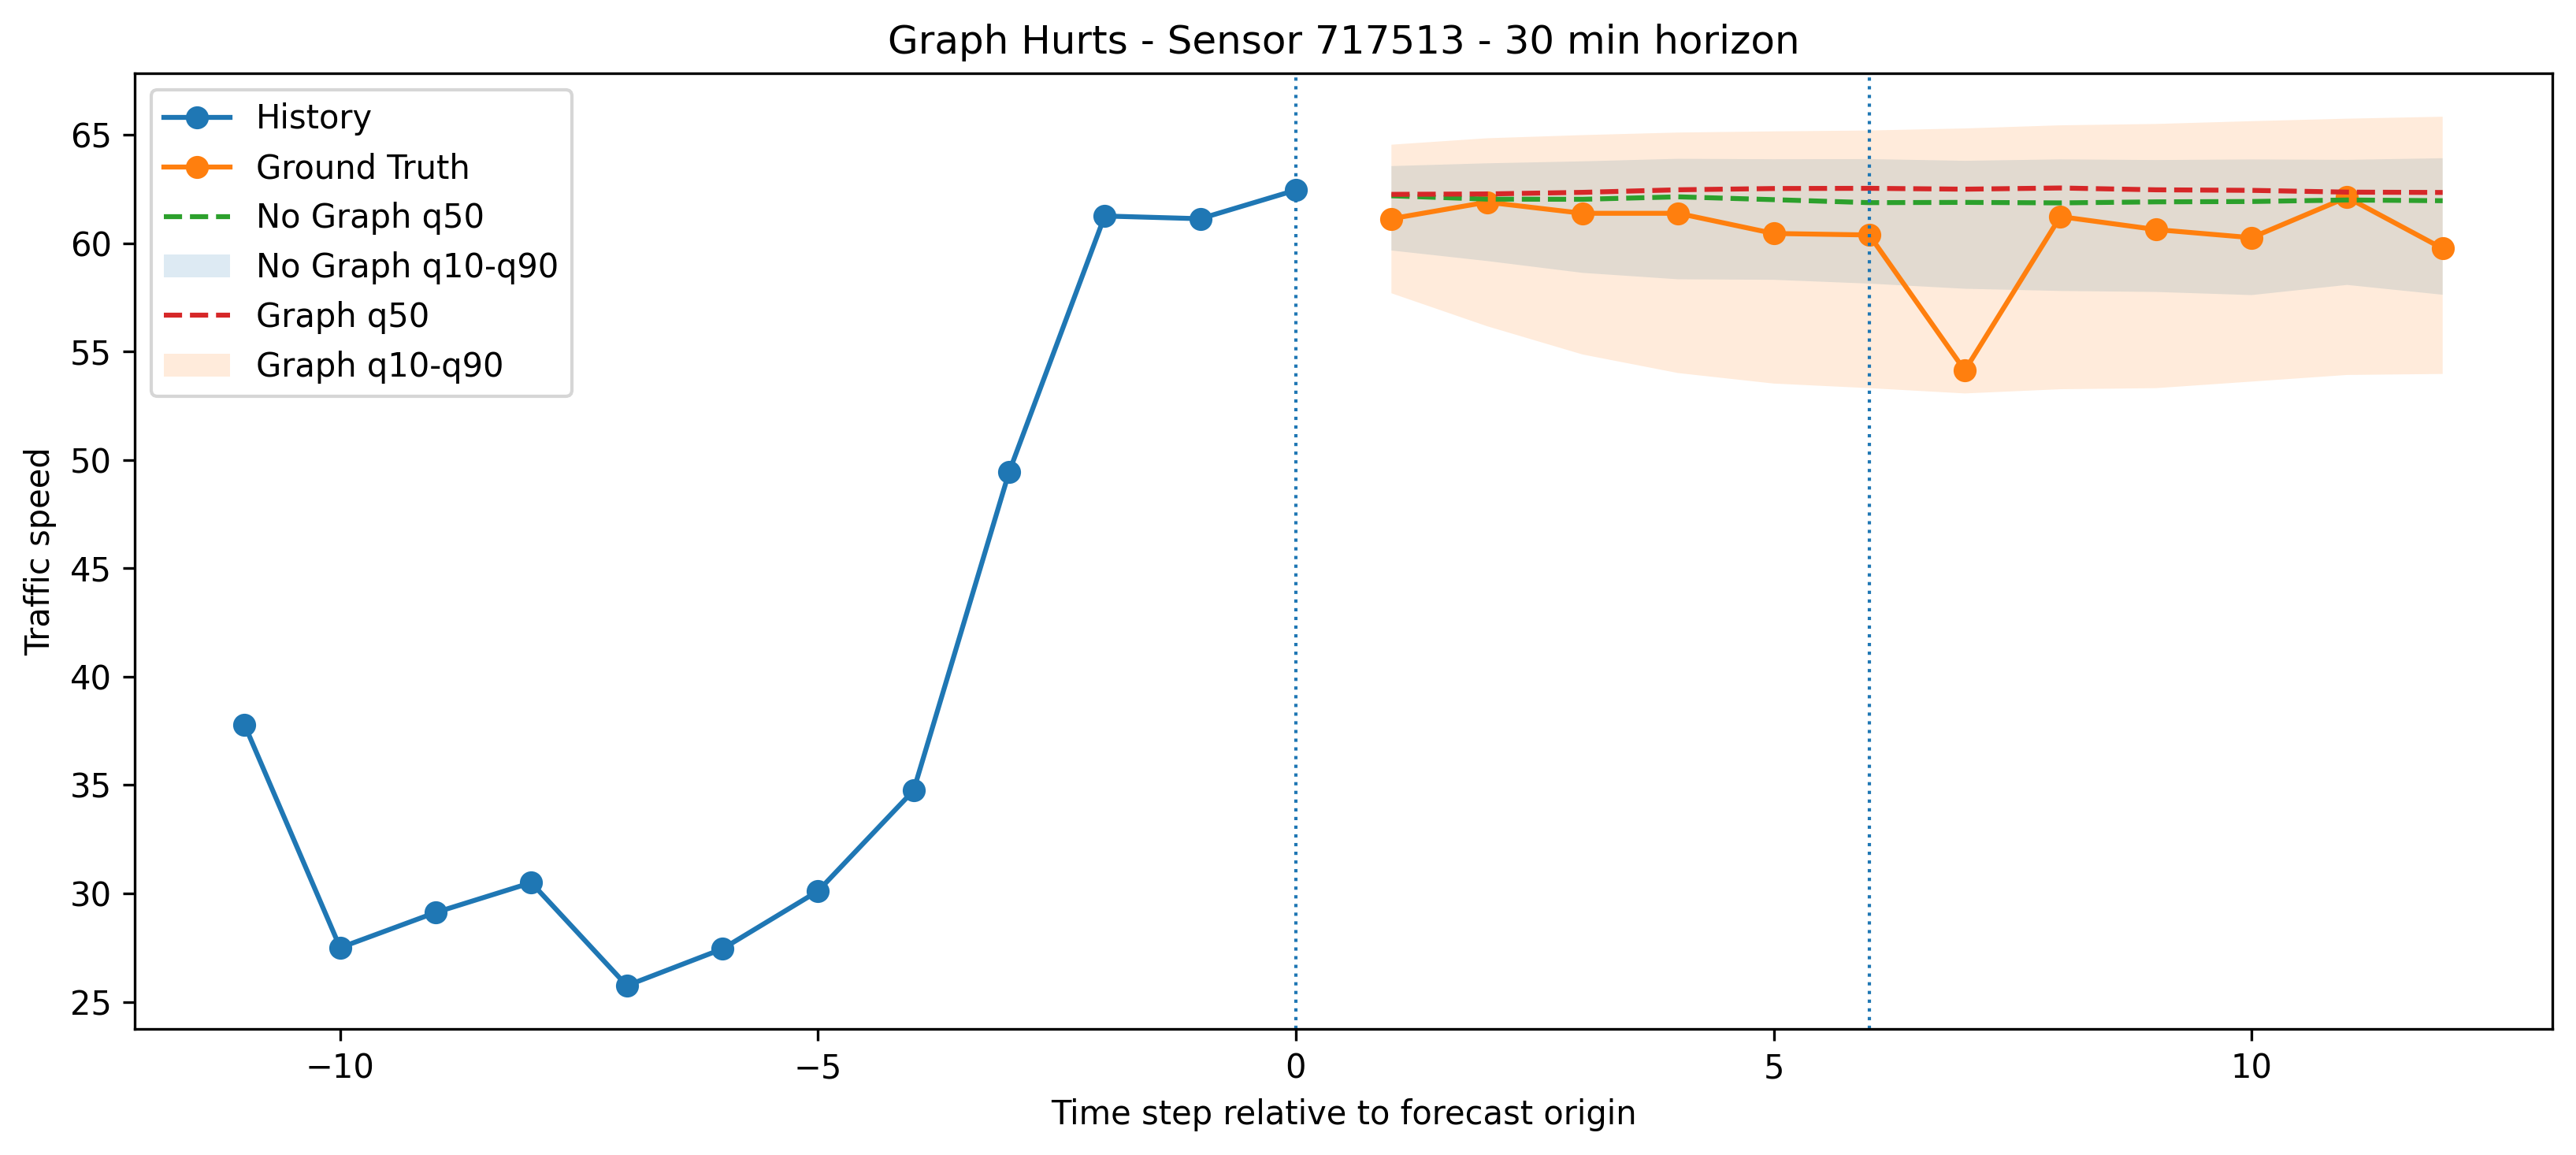
\includegraphics[width=\linewidth]{img/graph_impact_analysis/graph_hurts_h6_sensor_717513}
    \end{minipage}
    \hfill
    \begin{minipage}[b]{0.8\linewidth}
        \centering
        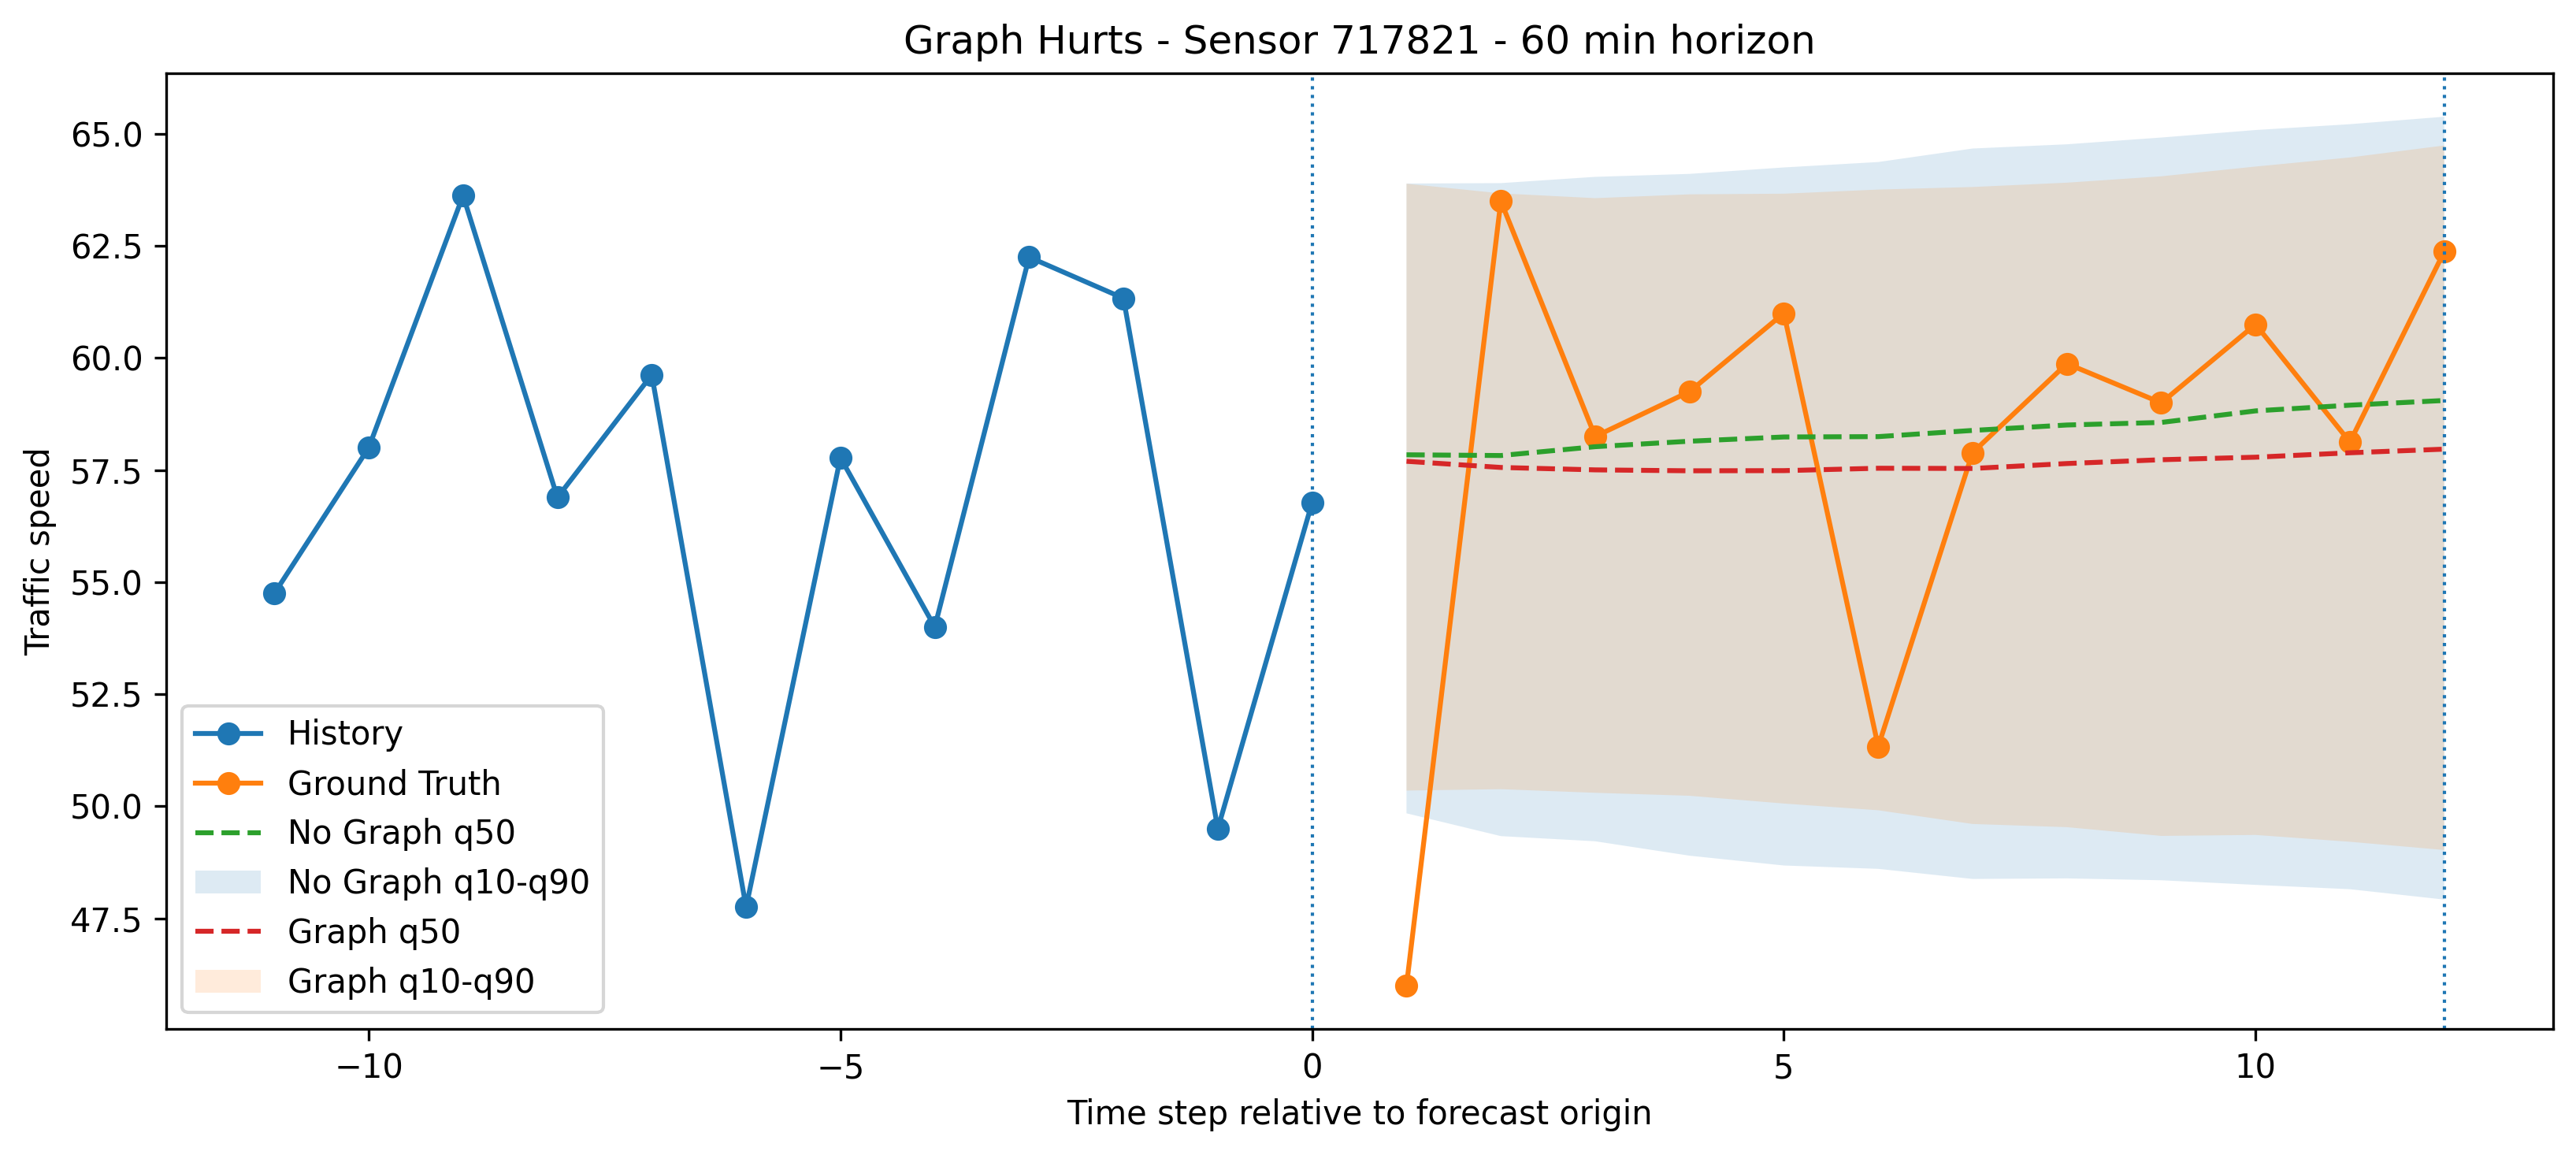
\includegraphics[width=\linewidth]{img/graph_impact_analysis/graph_hurts_h12_sensor_717821}
    \end{minipage}

    \caption{Representative forecasting examples in which the Graph-Temporal
model performs worse than the Temporal GRU at the 15-minute (left), 30-minute
(center), and 60-minute (right) forecasting horizons.}
    \label{fig:graph_hurt_examples}
\end{figure}

Overall, these examples confirm that the effect of graph message passing is
sensor- and time-dependent. Although spatial information improves forecasting
accuracy for the large majority of sensors, it can occasionally introduce
information that does not improve the local prediction. This observation is
consistent with the small subset of sensors for which the Temporal GRU
achieves lower MAE.

\subsection{Effect of Diffusion Depth}
\label{subsec:diffusion_depth}

The main Graph-Temporal model uses a diffusion depth of $K=2$, allowing each
diffusion layer to combine information from the current node and from nodes
reached through one and two-step propagation. To investigate whether a
larger spatial receptive field provides additional benefits, a variant with
$K=3$ was trained while keeping the remaining model configuration unchanged.

Table~\ref{tab:diffusion_depth} compares the test performance of the two
configurations. Increasing the diffusion depth produces a small but consistent
reduction in MAE. However, the same behavior
is not observed for RMSE since $K=3$ model obtains slightly higher RMSE at all
three horizons. Therefore, the additional diffusion step
slightly improves the average absolute error but does not improve the model's
sensitivity to larger forecasting errors.


\begin{table}[t]
    \centering
    \caption{Test performance of the Graph-Temporal model with diffusion
    depths $K=2$ and $K=3$.}
    \label{tab:diffusion_depth}
    \resizebox{\linewidth}{!}{
    \begin{tabular}{ccrrrrr}
        \toprule
        $K$ & Horizon &
        MAE & RMSE & Coverage (\%) & Interval Width & Crossing (\%) \\
        \midrule
        2 & 15 min & 2.901 & 5.511 & 78.44 & 8.929  & 0.031 \\
        2 & 30 min & 3.442 & 6.758 & 78.22 & 10.485 & 0.029 \\
        2 & 60 min & 4.244 & 8.378 & 78.13 & 12.470 & 0.048 \\
        \midrule
        3 & 15 min & 2.888 & 5.533 & 78.84 & 8.723  & 0.028 \\
        3 & 30 min & 3.424 & 6.799 & 77.87 & 9.948  & 0.034 \\
        3 & 60 min & 4.203 & 8.384 & 77.50 & 11.781 & 0.055 \\
        \bottomrule
    \end{tabular}}
\end{table}


\begin{figure}[t]
    \centering

    % First row: point forecasting metrics
    \begin{minipage}[b]{0.48\linewidth}
        \centering
        
\includegraphics[width=\linewidth]{img/graph_temporal/variant_comparison/mae_graph_temporal_variant_comparison}
    \end{minipage}
    \hfill
    \begin{minipage}[b]{0.48\linewidth}
        \centering
        
\includegraphics[width=\linewidth]{img/graph_temporal/variant_comparison/rmse_graph_temporal_variant_comparison}
    \end{minipage}

    \vspace{0.4cm}

    % Second row: probabilistic metrics
    \begin{minipage}[b]{0.48\linewidth}
        \centering
        
\includegraphics[width=\linewidth]{img/graph_temporal/variant_comparison//coverage_graph_temporal_variant_comparison}
    \end{minipage}
    \hfill
    \begin{minipage}[b]{0.48\linewidth}
        \centering
        
\includegraphics[width=\linewidth]{img/graph_temporal/variant_comparison/interval_width_graph_temporal_variant_comparison}
    \end{minipage}

    \caption{Comparison of the Graph-Temporal model with diffusion depths
    $K=2$ and $K=3$. The top row reports point forecasting performance in
    terms of MAE (left) and RMSE (right), while the bottom row reports
    empirical coverage (left) and prediction interval width (right) across
    the three forecasting horizons.}
    \label{fig:diffusion_depth_comparison}
\end{figure}

The comparison is also illustrated in
Figure~\ref{fig:diffusion_depth_comparison}. The effect of the additional
diffusion step is particularly visible in the probabilistic forecasts.
The $K=3$ model produces narrower prediction intervals at every horizon.
At the shortest horizon, this increased sharpness is accompanied by a small
improvement in coverage. At the longer forecasting horizons, however, the
sharper intervals obtained with $K=3$ come at the cost of increased
undercoverage. Quantile crossing remains negligible for both configurations.

The two configurations also exhibit different computational behavior. The
$K=2$ model was trained for 106 epochs, whereas the $K=3$ variant stopped
after 85 epochs. Despite requiring fewer epochs, the additional diffusion
step increases the computational cost of each epoch: the average training
time rises from approximately 19.3 seconds per epoch for $K=2$ to 22.0
seconds for $K=3$, an increase of about 14\%. The total training times are
approximately 34.0 and 31.1 minutes, respectively, with the lower total
training time of $K=3$ resulting from earlier stopping rather than lower
per-epoch computational complexity.

Overall, increasing the diffusion depth from $K=2$ to $K=3$ provides only
modest improvements in MAE and median Pinball Loss, while slightly increasing
RMSE and reducing coverage at the longer horizons. It also increases the
computational cost of each training epoch. For these reasons, $K=2$ was
retained for the main Graph-Temporal model, providing a more balanced
trade-off between forecasting accuracy, probabilistic reliability, and
computational complexity.

\subsection{Graph Ablation: Weighted vs. Binary Adjacency}
\label{subsec:weighted_binary}

The previous experiments use the original weighted adjacency matrix provided
with METR-LA. To investigate whether the edge weights contribute to the
forecasting performance or whether the graph connectivity alone is sufficient,
an ablation experiment was performed by replacing every non-zero edge weight
with one. The resulting binary adjacency matrix preserves the original graph
topology but removes information about the relative strength of the
connections. As for the weighted graph, the binary adjacency matrix was
row-normalized before being used for diffusion message passing.

Table~\ref{tab:weighted_binary} compares the two graph representations on the
test set. The weighted graph consistently achieves lower point forecasting
errors and the difference becomes larger as the forecasting horizon increases.


\begin{table}[t]
    \centering
    \caption{Test performance of the Graph-Temporal model using the weighted
    and binary adjacency matrices.}
    \label{tab:weighted_binary}
    \resizebox{\linewidth}{!}{
    \begin{tabular}{llrrrr}
        \toprule
        Graph & Horizon & MAE & RMSE & Coverage (\%) & Interval Width \\
        \midrule
        Weighted
        & 15 min & 2.901 & 5.511 & 78.44 & 8.929 \\
        & 30 min & 3.442 & 6.758 & 78.22 & 10.485 \\
        & 60 min & 4.244 & 8.378 & 78.13 & 12.470 \\
        \midrule
        Binary
        & 15 min & 2.948 & 5.682 & 79.54 & 8.878 \\
        & 30 min & 3.543 & 7.033 & 78.80 & 10.424 \\
        & 60 min & 4.443 & 8.754 & 78.11 & 12.593 \\
        \bottomrule
    \end{tabular}}
\end{table}


\begin{figure}[t]
    \centering

    % First row: point forecasting metrics
    \begin{minipage}[b]{0.48\linewidth}
        \centering
        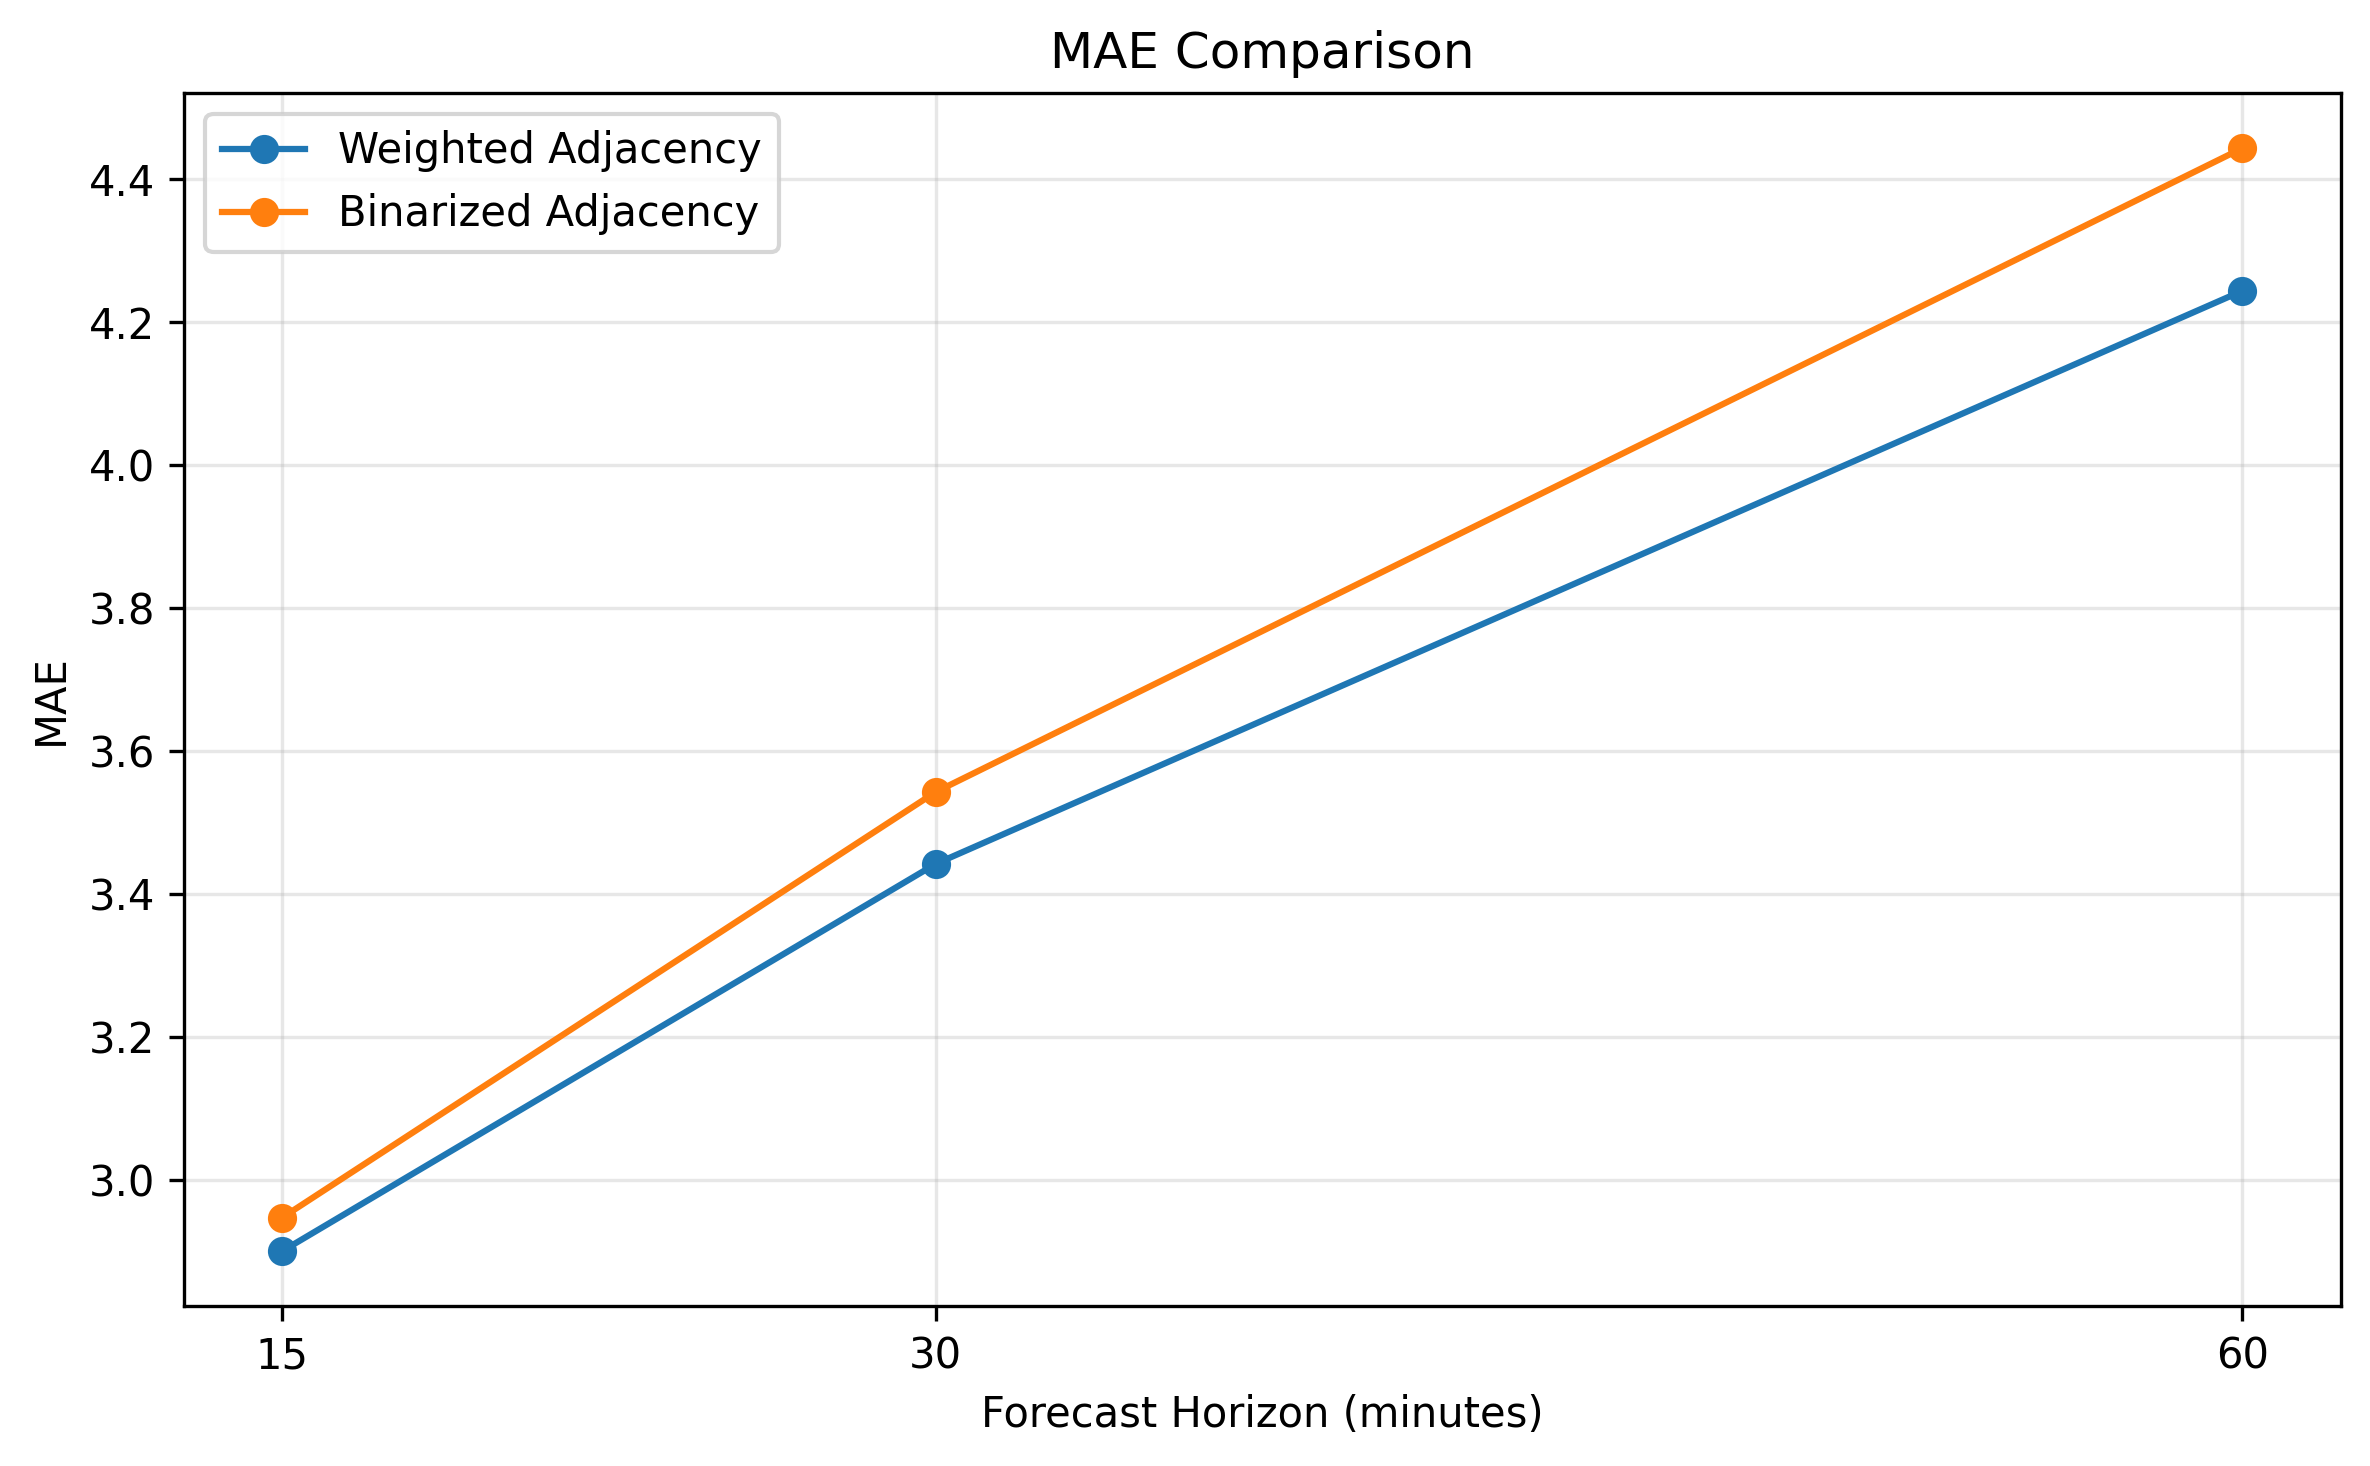
\includegraphics[width=\linewidth]{img/graph_temporal/ablation_comparison/mae_graph_temporal_variant_comparison}
    \end{minipage}
    \hfill
    \begin{minipage}[b]{0.48\linewidth}
        \centering
        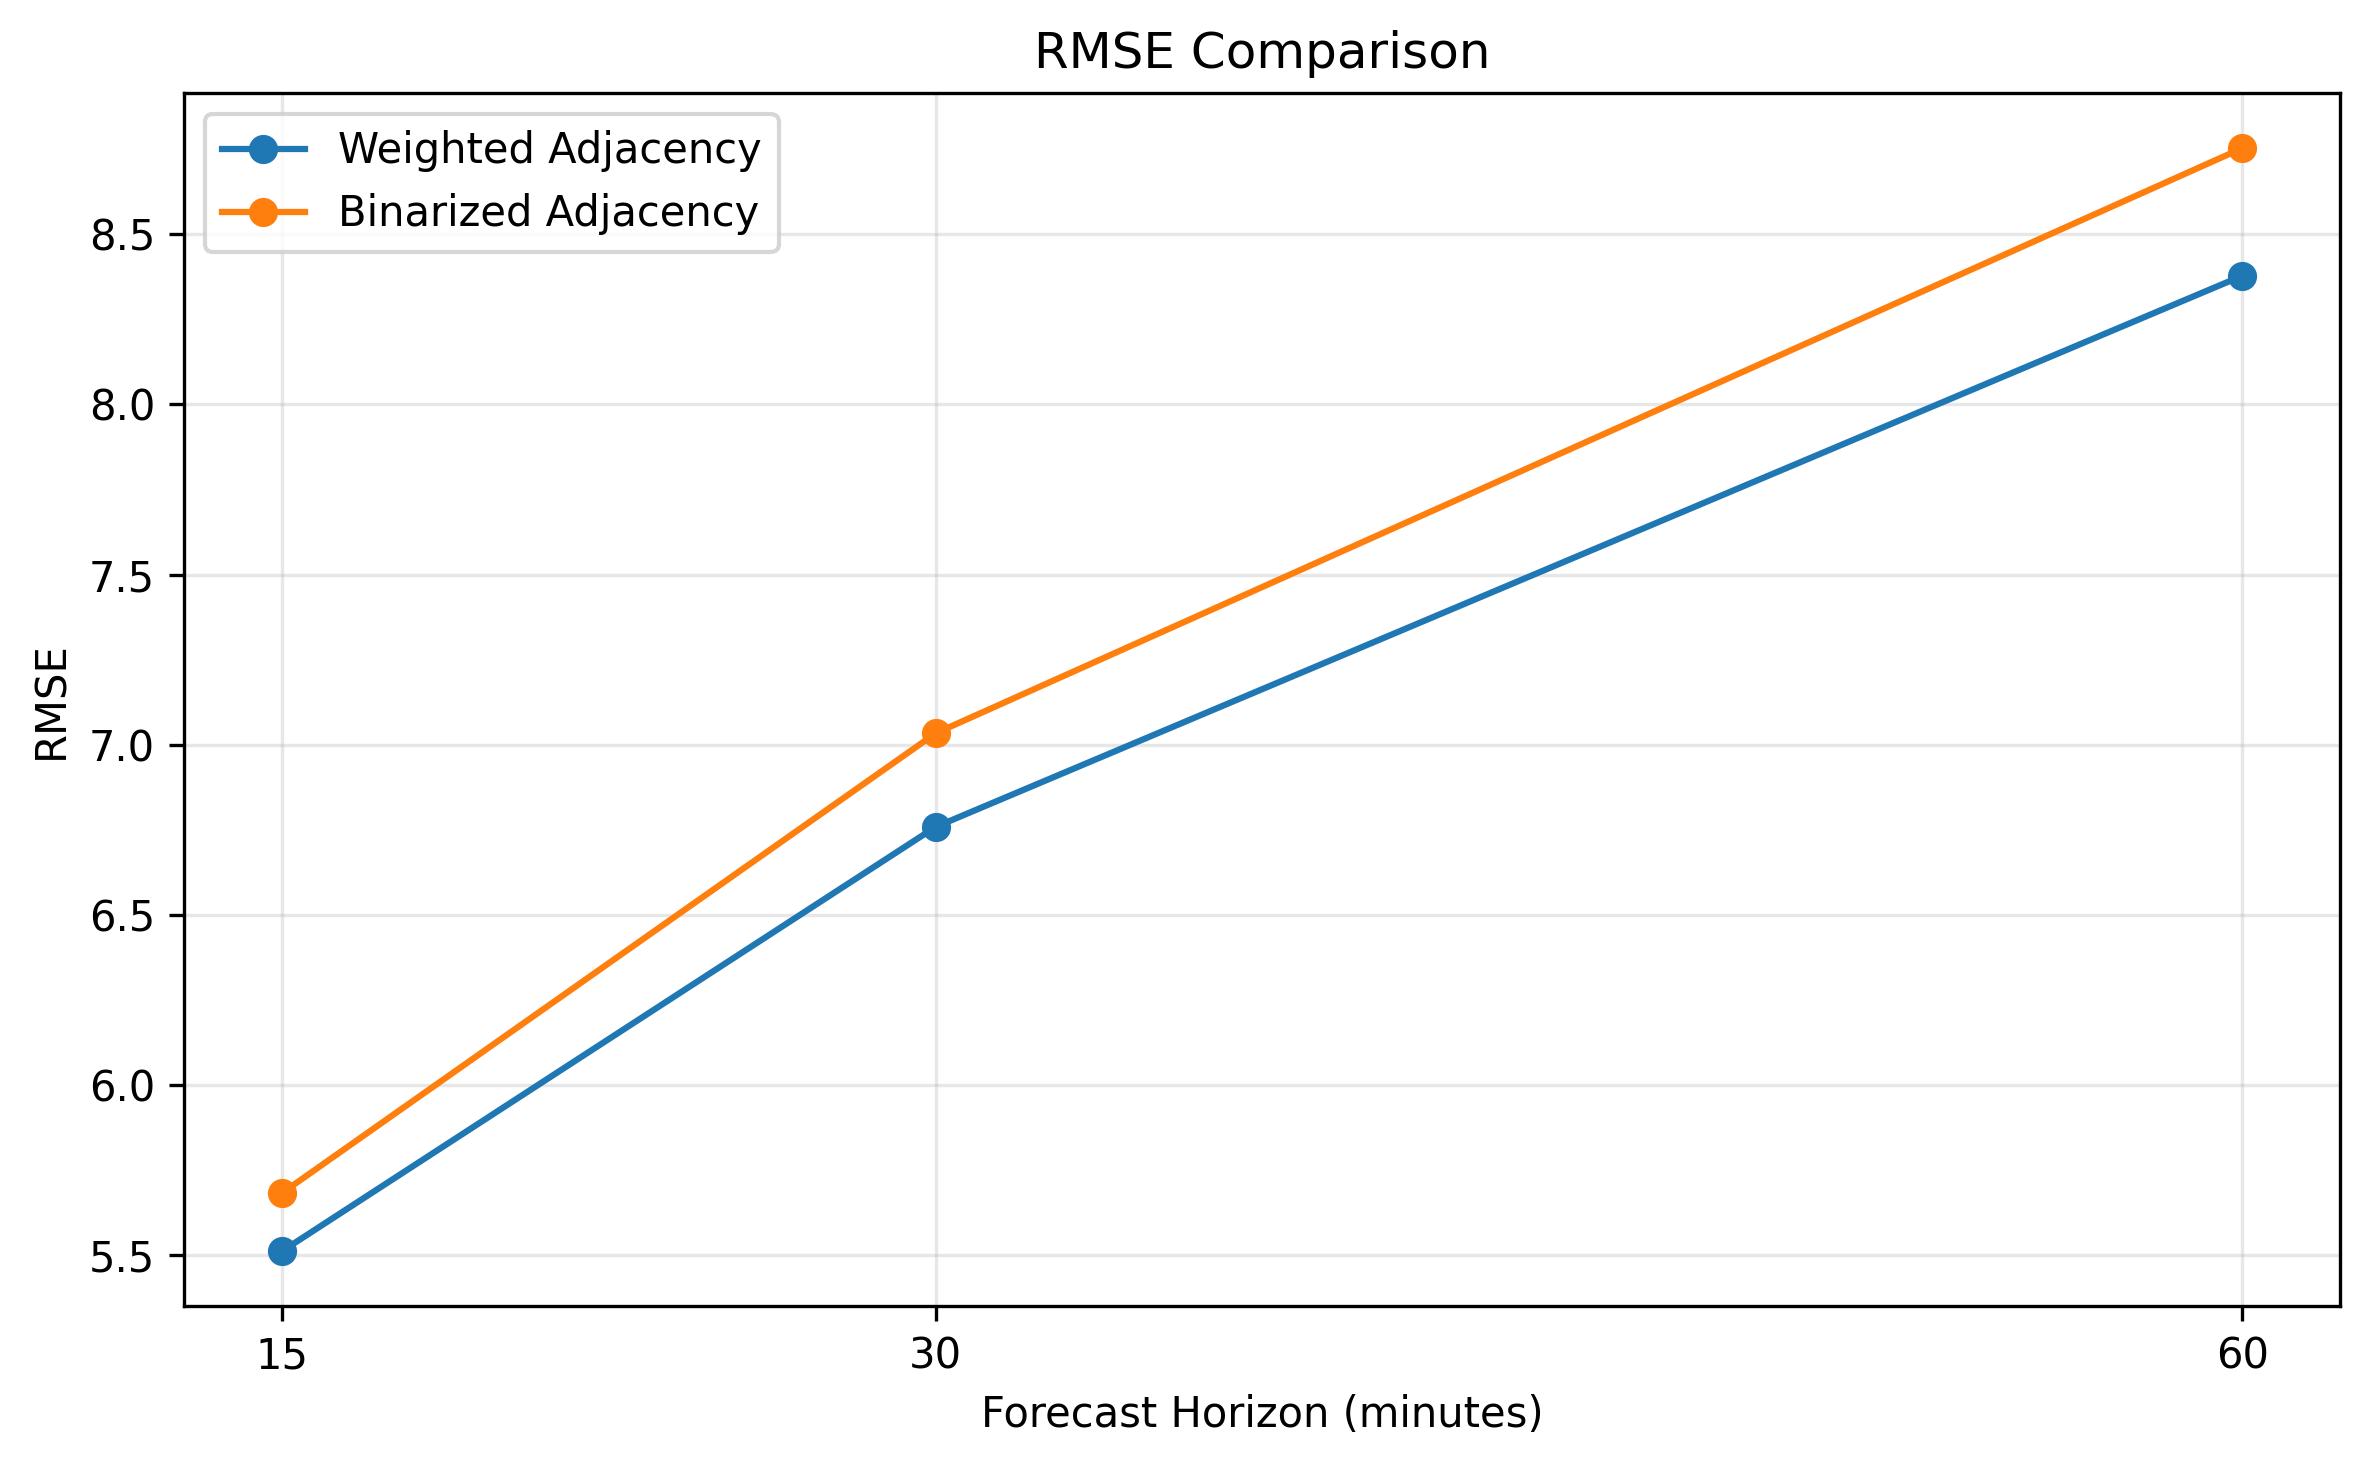
\includegraphics[width=\linewidth]{img/graph_temporal/ablation_comparison/rmse_graph_temporal_variant_comparison}
    \end{minipage}

    \vspace{0.4cm}

    % Second row: probabilistic metrics
    \begin{minipage}[b]{0.48\linewidth}
        \centering
        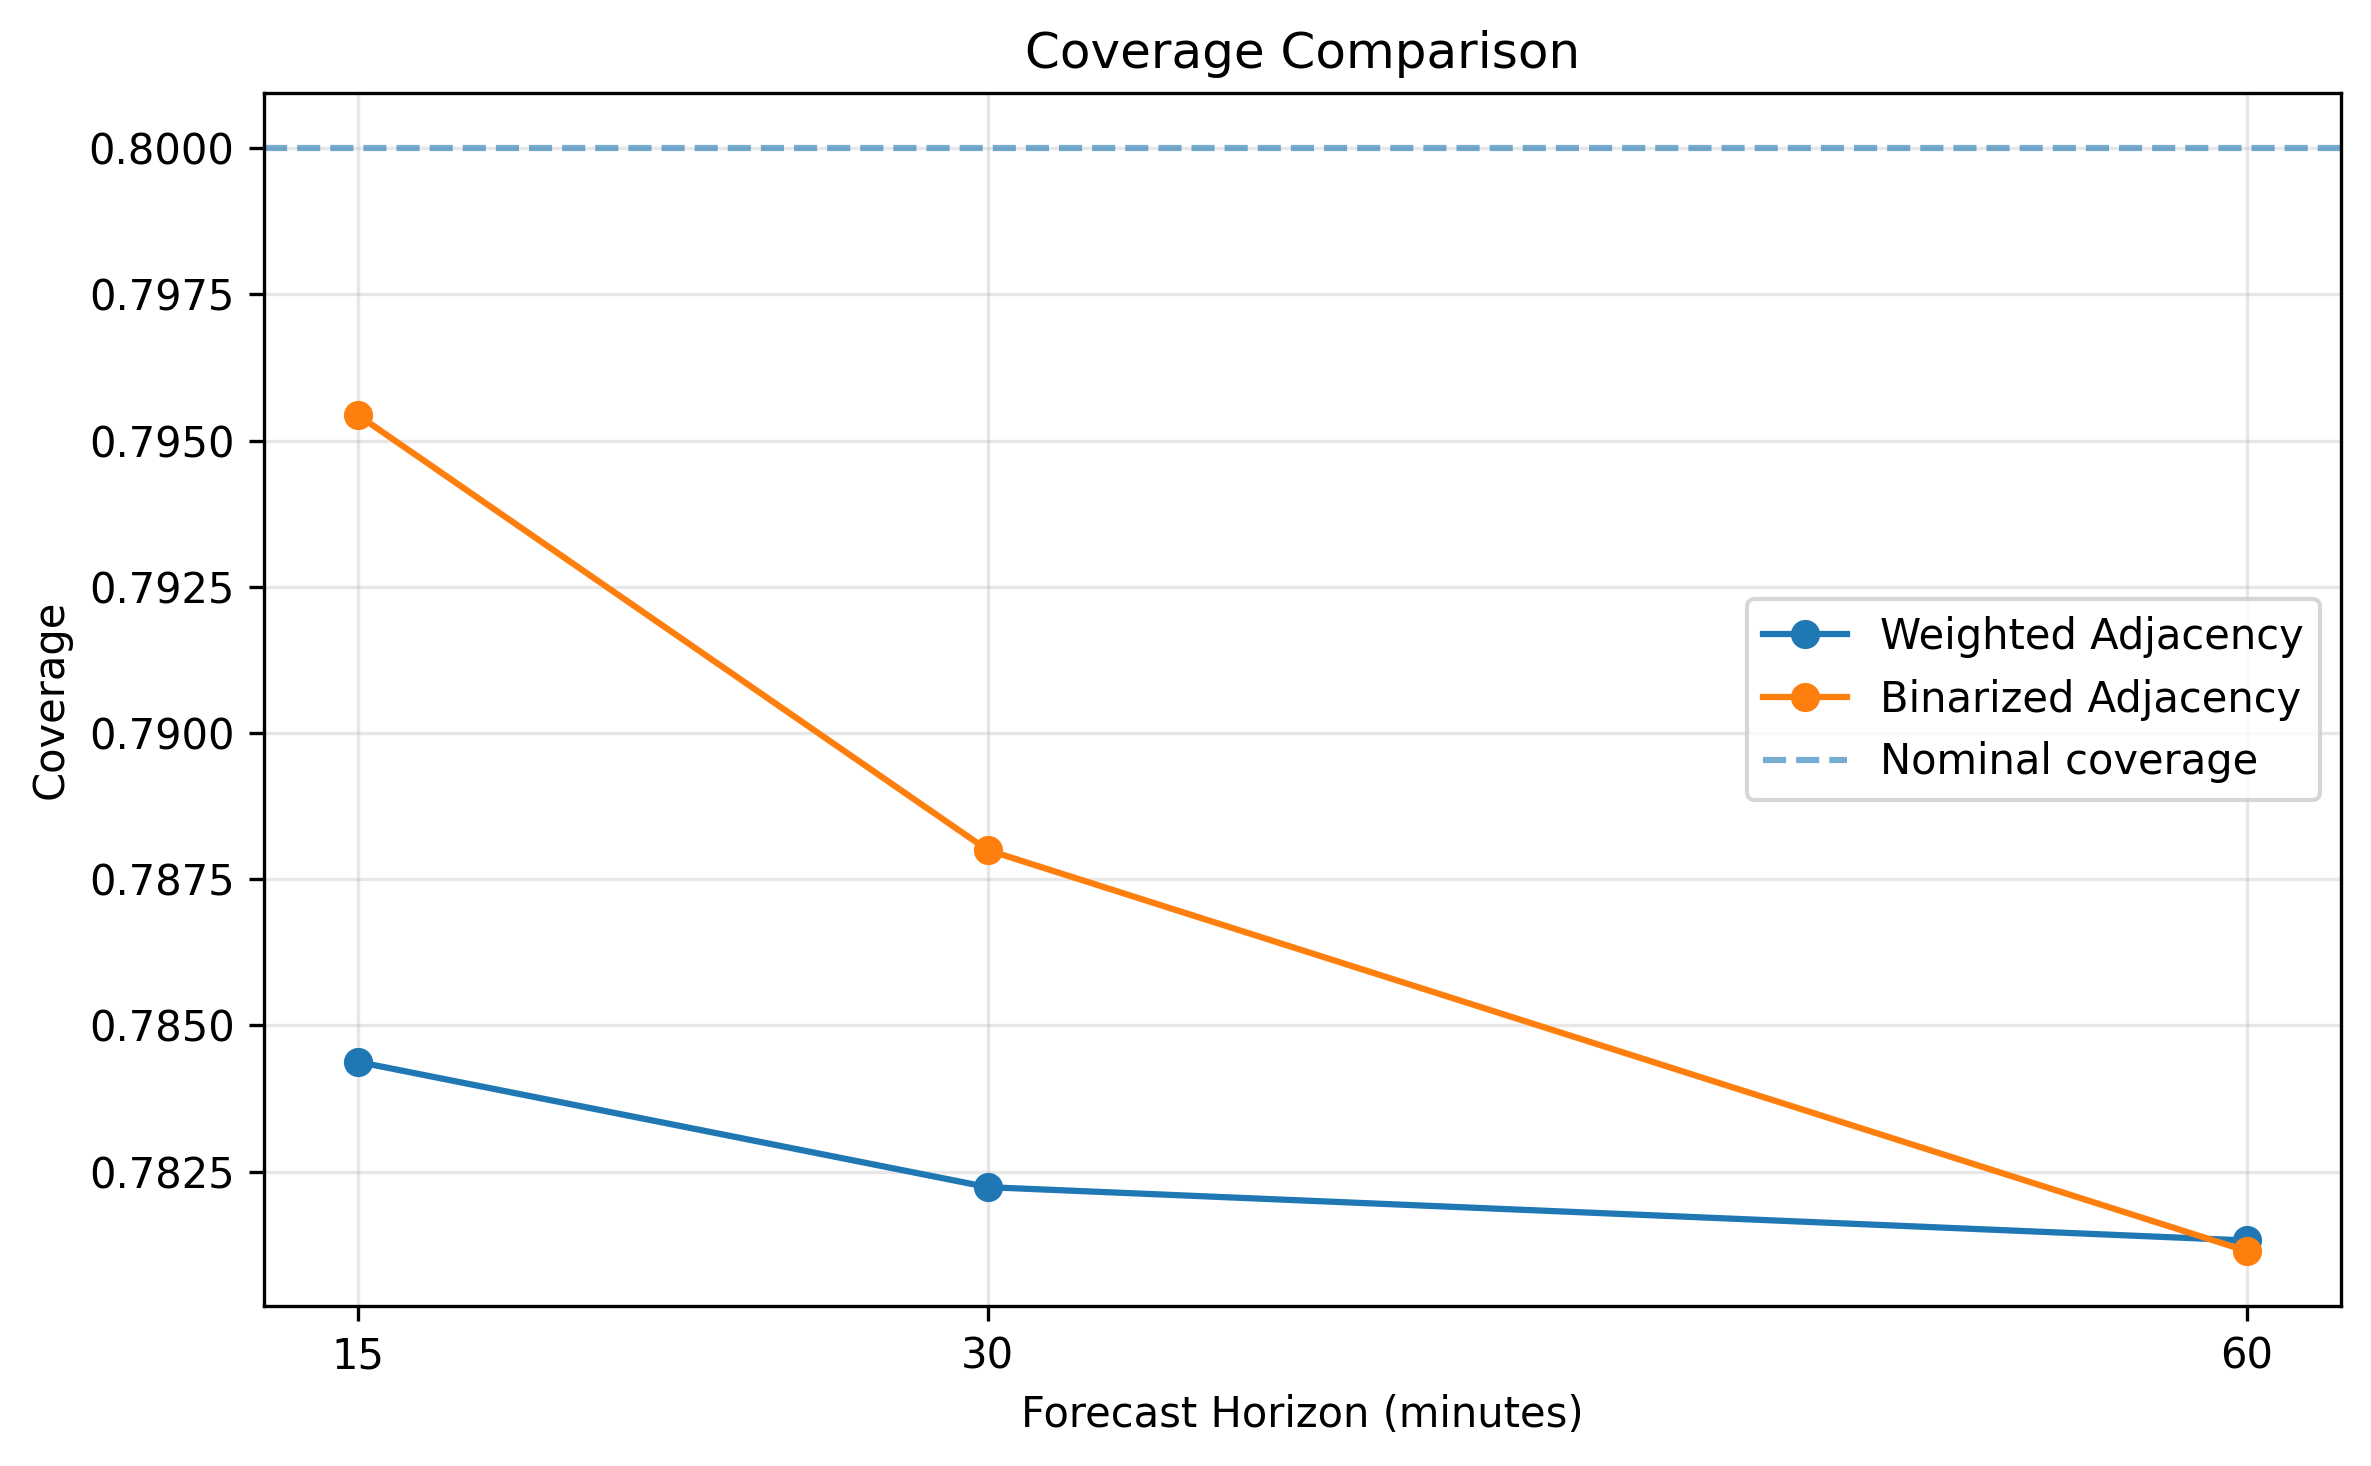
\includegraphics[width=\linewidth]{img/graph_temporal/ablation_comparison/coverage_graph_temporal_variant_comparison}
    \end{minipage}
    \hfill
    \begin{minipage}[b]{0.48\linewidth}
        \centering
        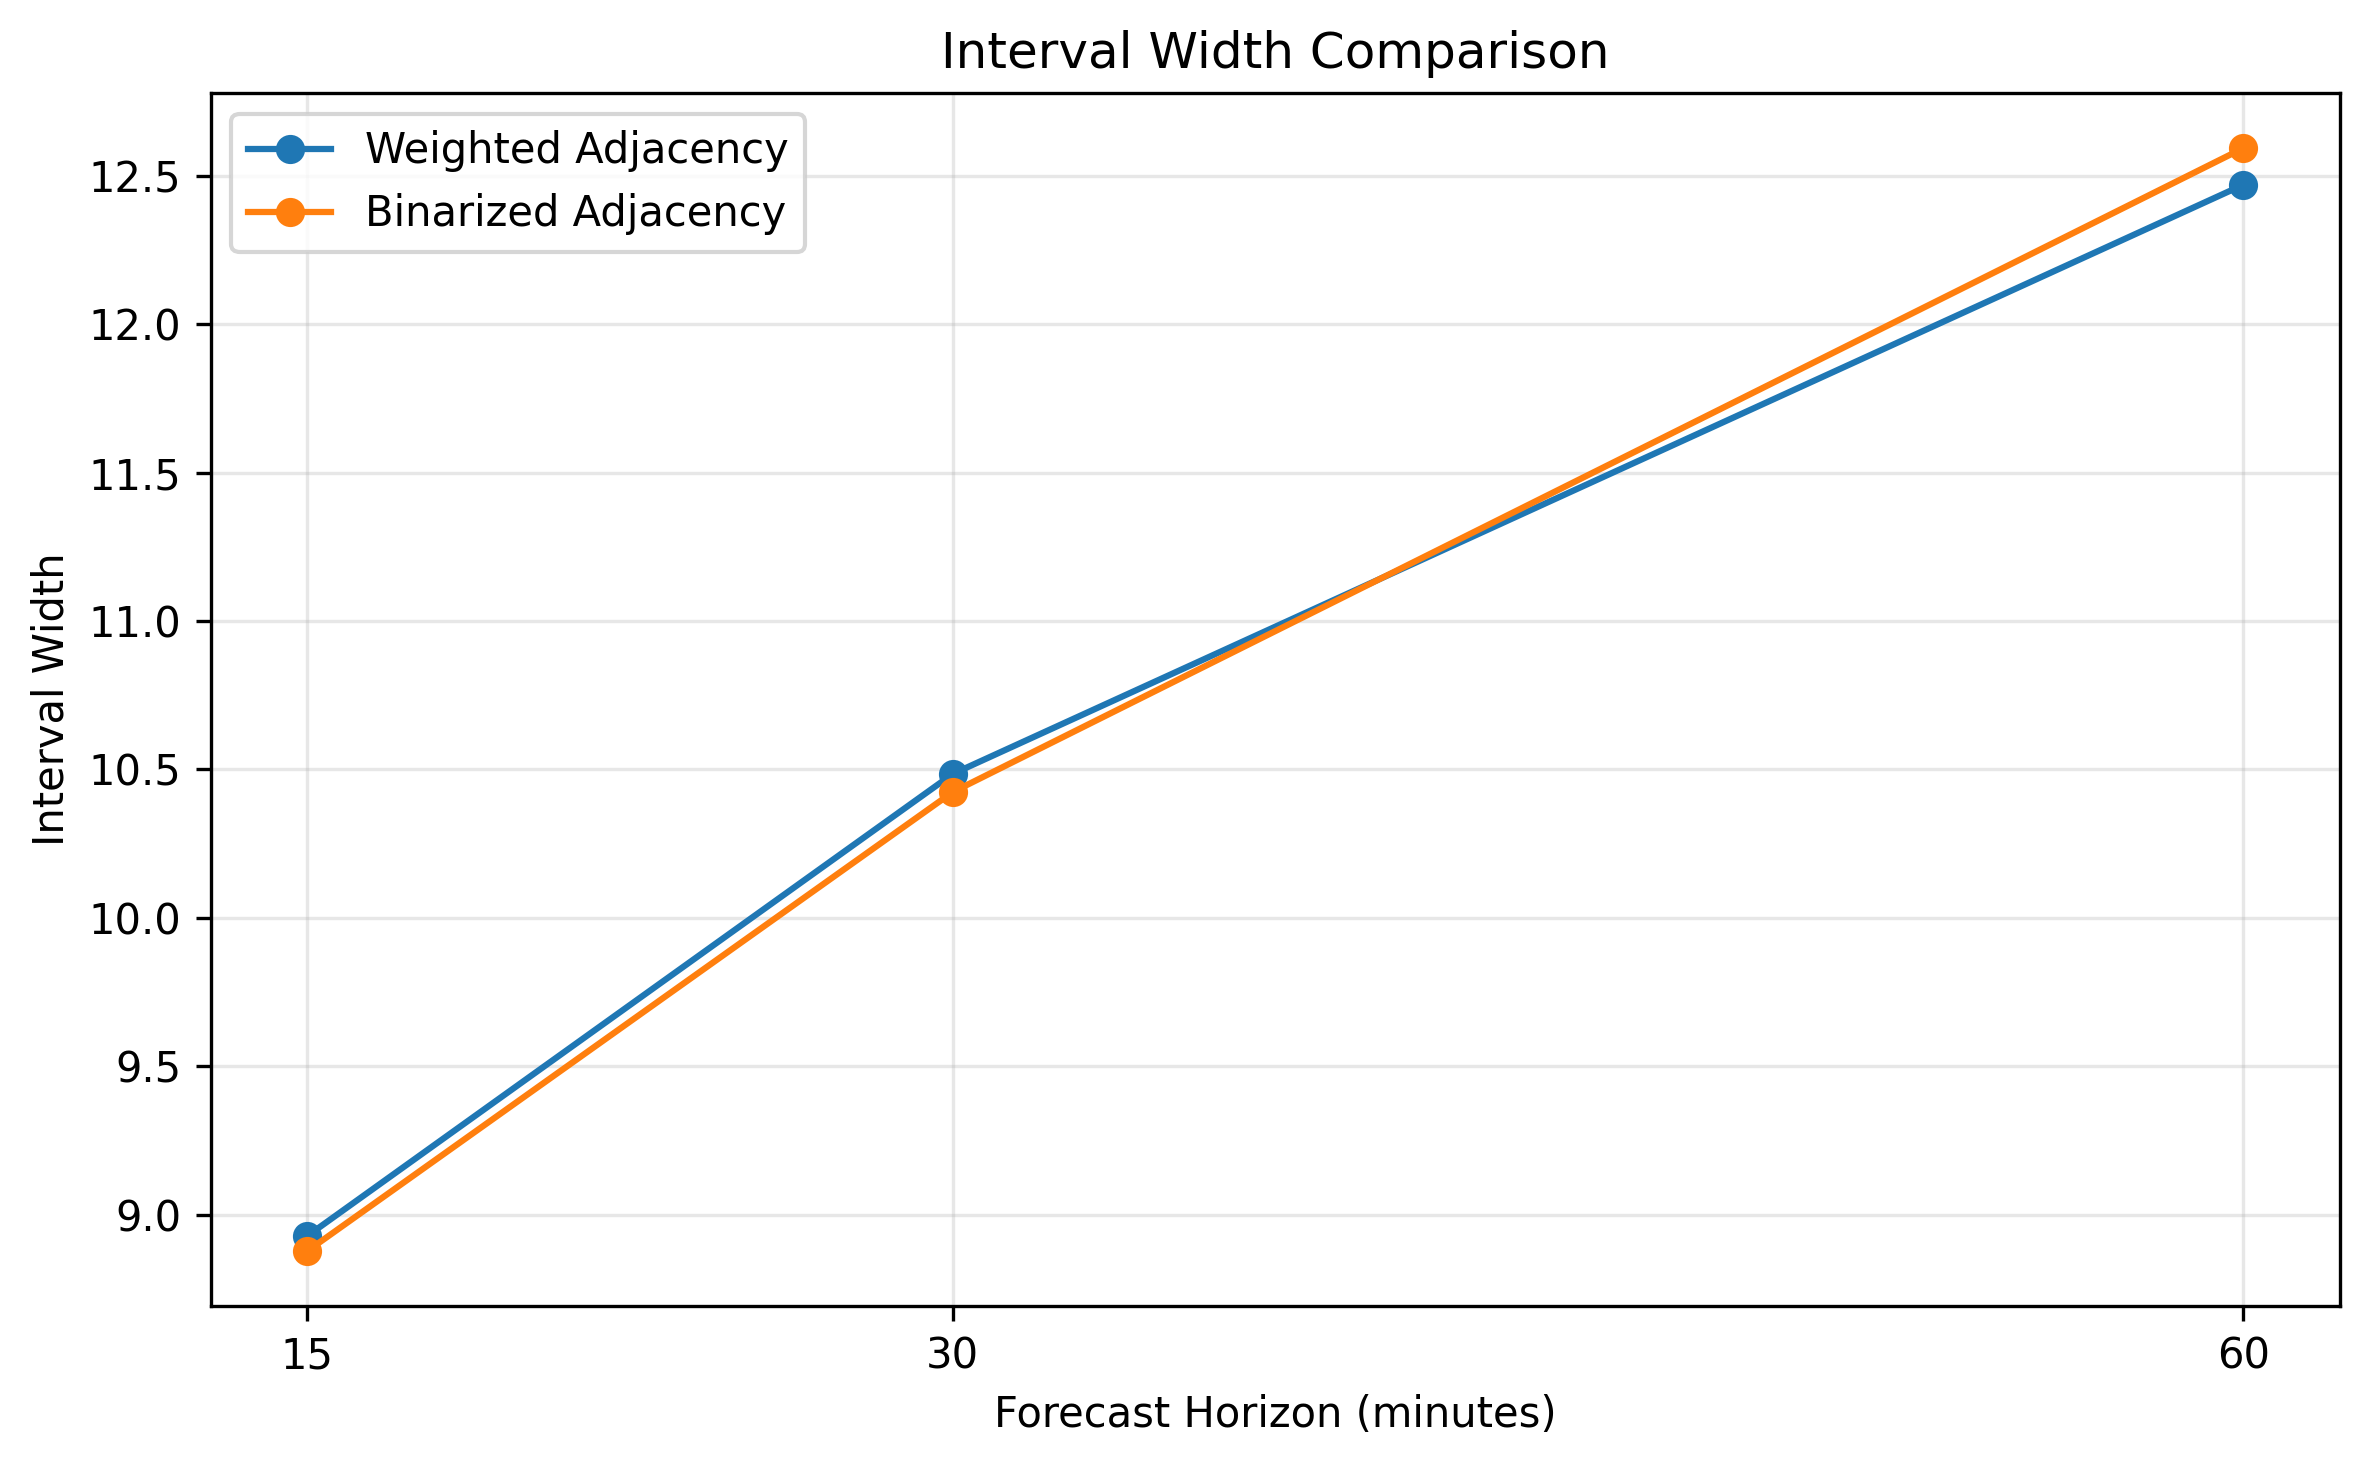
\includegraphics[width=\linewidth]{img/graph_temporal/ablation_comparison/interval_width_graph_temporal_variant_comparison}
    \end{minipage}

    \caption{Comparison of the Graph-Temporal model using the weighted and
    binary adjacency matrices. The top row reports point forecasting
    performance in terms of MAE (left) and RMSE (right), while the bottom
    row reports empirical coverage (left) and prediction interval width
    (right) across the three forecasting horizons.}
    \label{fig:weighted_binary_comparison}
\end{figure}

The comparison is further illustrated in
Figure~\ref{fig:weighted_binary_comparison}. The probabilistic results reveal
a more nuanced difference. At 15 and 30 minutes, the binary graph produces
slightly narrower intervals, while its empirical coverage is slightly closer
to the nominal 80\% level. At 60 minutes, however, the binary representation
produces a slightly wider interval, while coverage remains almost unchanged.
Therefore, binarizing the graph does not provide a consistent advantage in
terms of interval sharpness or reliability.


Overall, these results indicate that the benefit of graph message passing is
not determined solely by the presence of connections between sensors. The
relative edge weights provide useful information for spatial aggregation,
with their contribution becoming more evident as the forecasting horizon
increases. Since the binary graph does not provide a consistent improvement
in probabilistic reliability and results in higher point errors,
the original weighted adjacency matrix was retained for the main
Graph-Temporal model.
%\section{Robustness under Distribution Shift}
\label{sec:distribution_shift}

The previous experiments evaluate forecasting performance over the complete
test distribution. However, average performance may hide substantial
degradation under traffic conditions that are less frequently represented
during training. To investigate this aspect, the Graph-Temporal model is
evaluated under a predefined high-congestion stress condition. The stress
condition is defined exclusively from the training data, preventing
information from the validation or test sets from influencing the definition
of the shifted subset.

\subsection{High-Congestion Definition}
\label{subsec:congestion_definition}

High-congestion conditions are identified using sensor-specific speed
thresholds. For each sensor $n$, a congestion threshold $\tau_n$ is defined
as the 10th percentile of its valid speed observations in the training set,

\begin{equation}
    \tau_n =
    Q_{0.10}
    \left(
        \left\{y_{t,n}^{\mathrm{train}} :
        m_{t,n}^{\mathrm{train}} = 1\right\}
    \right),
    \label{eq:sensor_congestion_threshold}
\end{equation}

where $m_{t,n}^{\mathrm{train}}$ denotes the availability mask. A sensor is
therefore considered congested at time $t$ when its valid observed speed is
lower than or equal to its sensor-specific threshold. Using a separate
threshold for each sensor accounts for the different typical speed ranges
observed across locations in the road network.

The network-level congestion ratio at timestamp $t$ is then defined as the
fraction of valid sensors that are classified as congested,

\begin{equation}
    C_t =
    \frac{
        \sum_{n=1}^{N}
        m_{t,n}\,
        \mathbb{I}\!\left(y_{t,n} \leq \tau_n\right)
    }{
        \sum_{n=1}^{N} m_{t,n}
    },
    \label{eq:congestion_ratio}
\end{equation}

where $\mathbb{I}(\cdot)$ is the indicator function. This definition measures
the spatial extent of congestion at each timestamp rather than relying on the
speed of a single sensor.

Finally, the threshold used to identify a high-congestion event is defined
as the 95th percentile of the congestion ratios observed in the training
set,

\begin{equation}
    \tau_{\mathrm{peak}}
    =
    Q_{0.95}
    \left(
        \left\{C_t^{\mathrm{train}}\right\}
    \right).
    \label{eq:peak_threshold}
\end{equation}

For the METR-LA training partition, this procedure yields
$\tau_{\mathrm{peak}} = 0.3495$. Consequently, a timestamp is classified as
a high-congestion condition when at least approximately 35\% of the valid
sensors simultaneously exhibit speeds below their respective training-based
10th-percentile thresholds.

\begin{figure}[t]
    \centering
    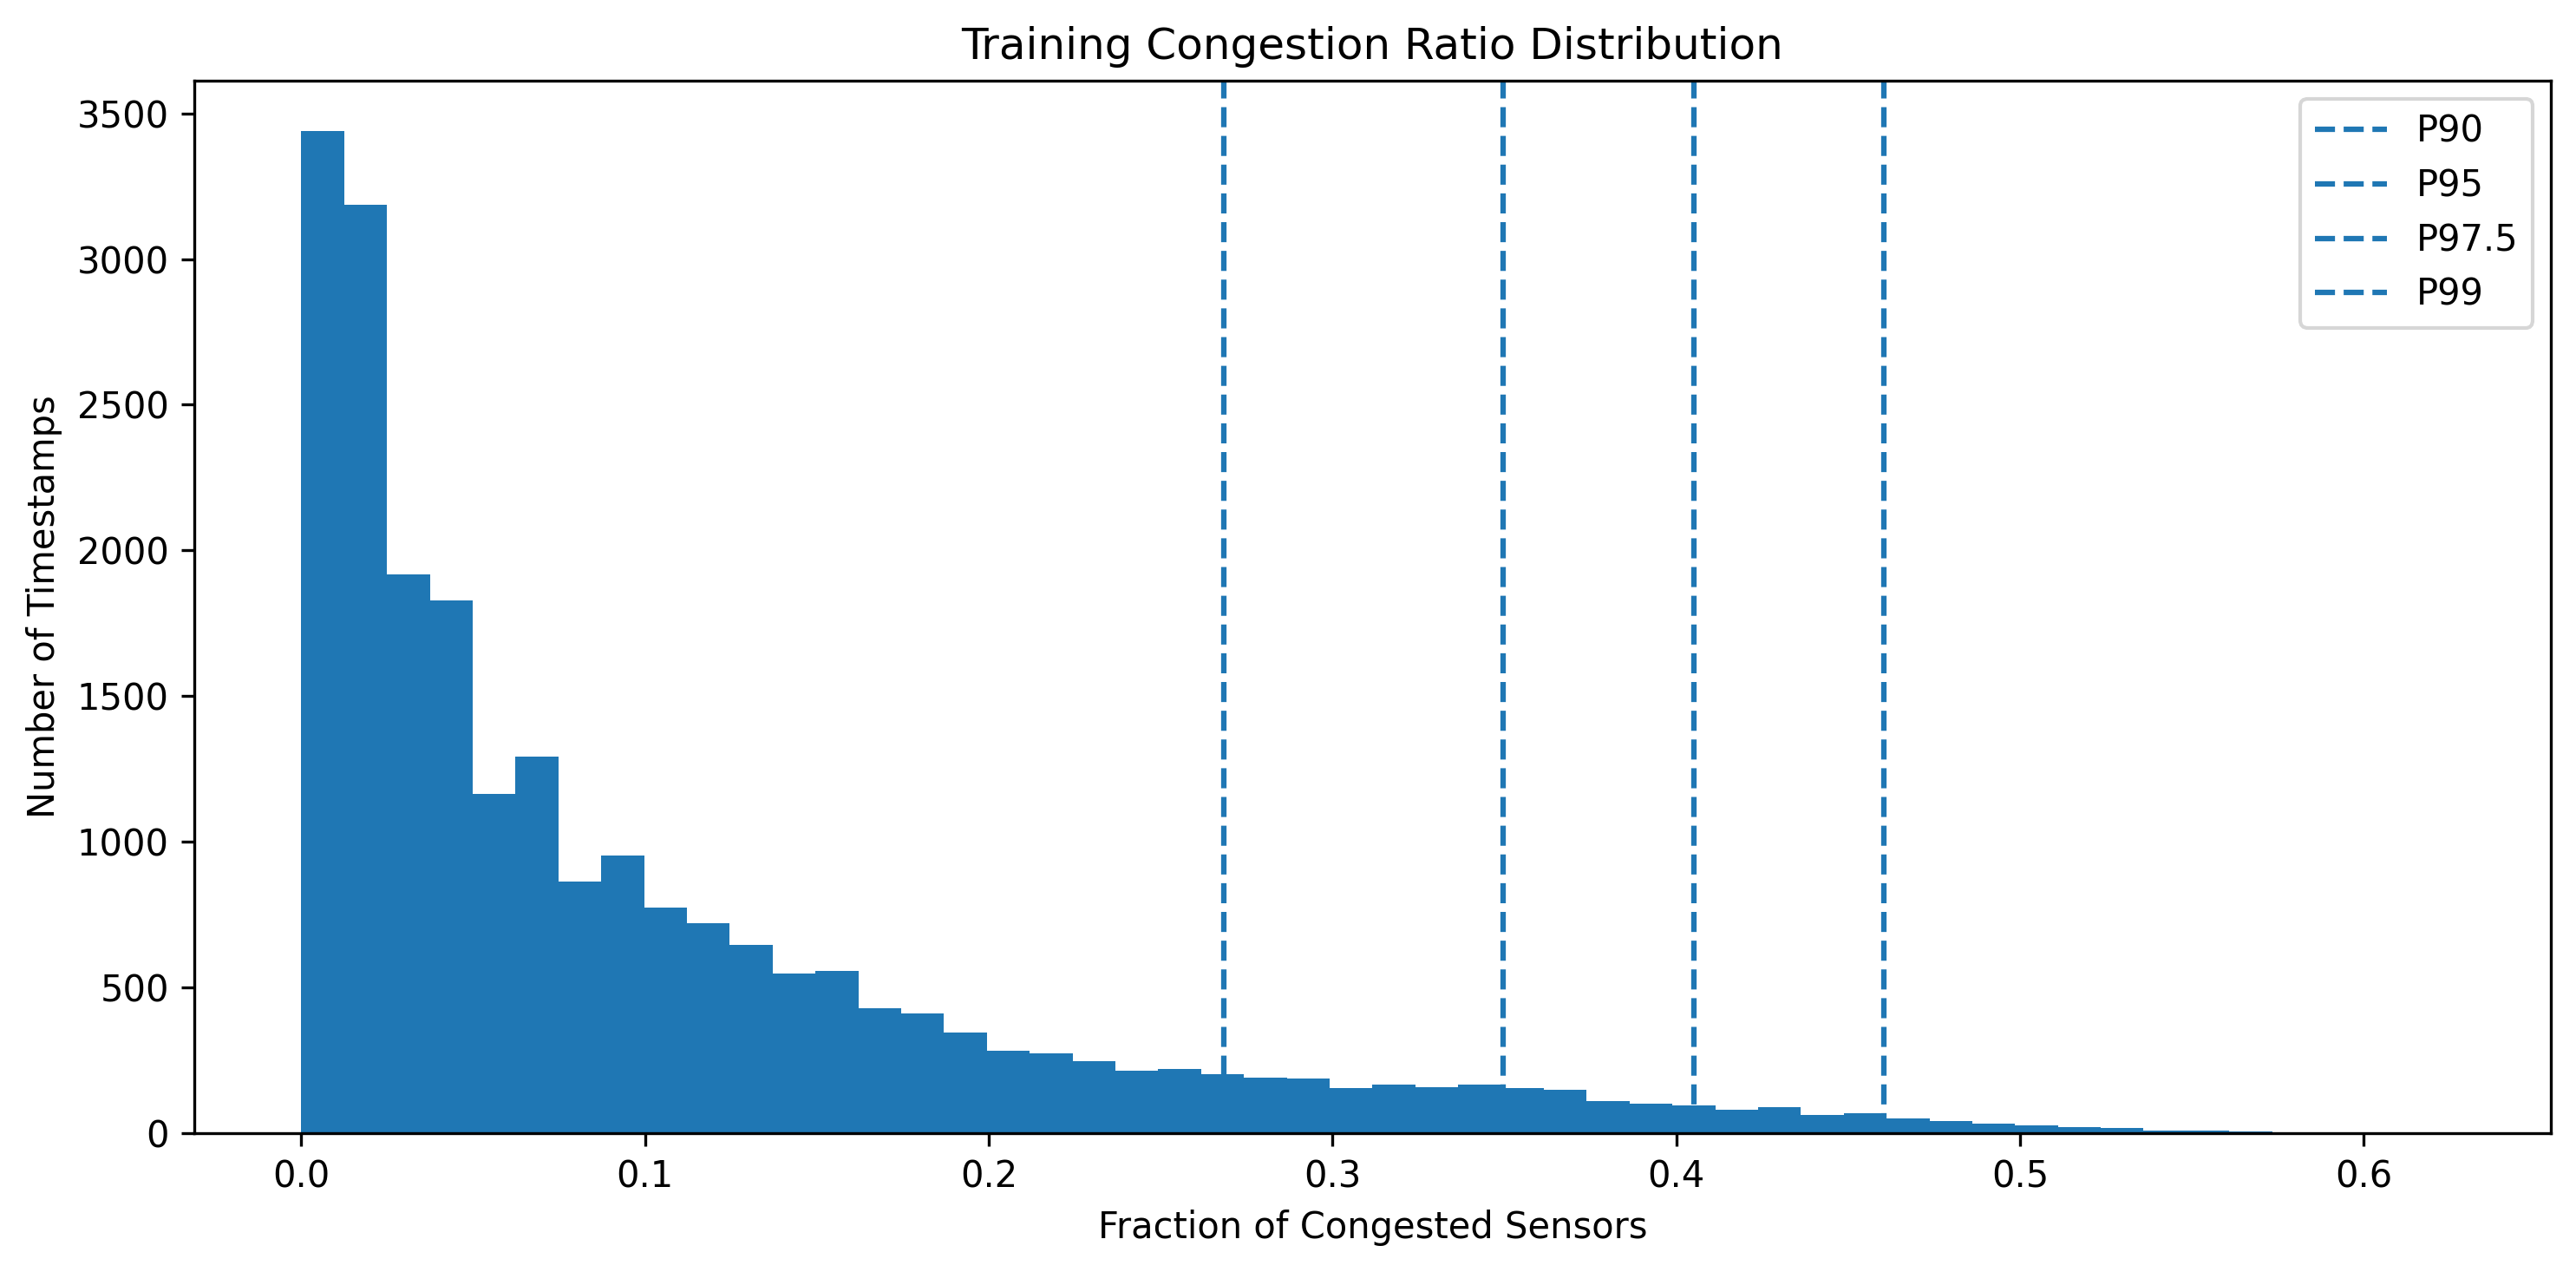
\includegraphics[width=0.75\linewidth]
    {img/distribution_shift/congestion_ratio_distribution}
    \caption{Distribution of the network-level congestion ratio $C_t$ in the
    training set.}
    \label{fig:congestion_ratio_distribution}
\end{figure}

Figure~\ref{fig:congestion_ratio_distribution} shows the training
distribution used to define the stress condition. By selecting its 95th
percentile, the stress test focuses on relatively uncommon periods in which
congestion simultaneously affects a substantial fraction of the network.
Importantly, both the sensor-specific thresholds $\tau_n$ and the
network-level threshold $\tau_{\mathrm{peak}}$ are estimated exclusively
from the training partition and subsequently kept fixed when classifying
validation and test observations.


\subsection{Stress-Test Protocol}
\label{subsec:stress_protocol}

The high-congestion definition introduced in
Section~\ref{subsec:congestion_definition} is applied to the forecasting
targets of each test window. Since the model is evaluated at three different
forecasting horizons, congestion is assessed independently at the target
timestamp corresponding to each horizon.

More specifically, for a test sample whose input sequence ends at time $t$,
the congestion condition for forecasting horizon $h$ is determined from the
network-level congestion ratio at the corresponding future timestamp
$t+h$. The sample is classified as high congestion for horizon $h$ when

\begin{equation}
    C_{t+h} \geq \tau_{\mathrm{peak}},
    \label{eq:high_congestion_sample}
\end{equation}

where $\tau_{\mathrm{peak}}=0.3495$ is the threshold estimated exclusively
from the training partition. Otherwise, the sample is assigned to the normal
subset for that horizon.

This horizon-specific classification is necessary because traffic conditions
may change within the 60-minute forecasting window. Consequently, the same
input window can be classified as normal at one forecasting horizon and as
high congestion at another. The stress-test subsets for 15, 30, and
60 minutes should therefore be interpreted independently rather than as a
single fixed set of test windows.

Applying this procedure to the 6224 test windows yields 484 high-congestion
samples and 5740 normal samples at each evaluated horizon. Although the
subset sizes are identical, their composition differs across horizons. For
example, the high-congestion masks have a Jaccard similarity of 0.741 between
15 and 30 minutes, 0.579 between 30 and 60 minutes, and 0.449 between
15 and 60 minutes. This decreasing overlap is expected because the target
timestamps become progressively farther apart.

The stress test evaluates the same trained Graph-Temporal model used in the
previous experiments, without retraining or adapting it to high-congestion
conditions. Forecasting metrics are computed separately over the normal and
high-congestion subsets using the target availability mask. This allows the
degradation associated with the shifted traffic condition to be measured
while keeping the model, preprocessing pipeline, and evaluation procedure
unchanged.

\subsection{Quantitative Results}
\label{subsec:shift_quantitative}

Table~\ref{tab:congestion_results} reports the performance of the
Graph-Temporal model separately under normal and high-congestion conditions.
A substantial degradation is observed under high congestion at all three
forecasting horizons, and the difference becomes progressively larger as the
prediction horizon increases.

\begin{table}[t]
    \centering
    \caption{Performance of the Graph-Temporal model under normal and
    high-congestion conditions on the test set.}
    \label{tab:congestion_results}
    \begin{tabular}{llrrrr}
        \toprule
        Condition & Horizon &
        MAE & RMSE & Coverage (\%) & Interval Width \\
        \midrule
        Normal
        & 15 min & 2.770 & 5.289 & 78.4 & 8.499 \\
        & 30 min & 3.257 & 6.453 & 78.3 & 9.911 \\
        & 60 min & 3.974 & 7.957 & 78.3 & 11.730 \\
        \midrule
        High congestion
        & 15 min & 4.463 & 7.669 & 78.7 & 14.035 \\
        & 30 min & 5.636 & 9.660 & 77.9 & 17.283 \\
        & 60 min & 7.414 & 12.296 & 75.8 & 21.169 \\
        \bottomrule
    \end{tabular}
\end{table}

It is worth noting that the performance observed under normal conditions is
close to the overall test performance reported in
Section~\ref{sec:in_distribution_results}. This is expected from the
definition of the stress condition. High congestion is intentionally defined
as a relatively rare event through the 95th percentile of the training
congestion-ratio distribution and accounts for only 484 out of 6,224 test
windows, approximately 7.8\%, at each forecasting horizon. Consequently,
the overall test metrics are dominated by the much larger normal subset and
can therefore conceal the substantially poorer performance observed during
high-congestion periods.

\begin{figure}[t]
    \centering

    % First row: point forecasting metrics
    \begin{minipage}[b]{0.48\linewidth}
        \centering
        
\includegraphics[width=\linewidth]
        {img/distribution_shift/mae_distribution_shift}
    \end{minipage}
    \hfill
    \begin{minipage}[b]{0.48\linewidth}
        \centering
        
\includegraphics[width=\linewidth]
        {img/distribution_shift/rmse_distribution_shift}
    \end{minipage}

    \vspace{0.4cm}

    % Second row: probabilistic metrics
    \begin{minipage}[b]{0.48\linewidth}
        \centering
        
\includegraphics[width=\linewidth]
        {img/distribution_shift/coverage_distribution_shift}
    \end{minipage}
    \hfill
    \begin{minipage}[b]{0.48\linewidth}
        \centering
        
\includegraphics[width=\linewidth]
        {img/distribution_shift/interval_width_distribution_shift}
    \end{minipage}

    \caption{Performance of the Graph-Temporal model under normal and
    high-congestion conditions. The top row compares MAE (left) and RMSE
    (right), while the bottom row reports empirical coverage (left) and
    prediction interval width (right) across the three forecasting horizons.}
    \label{fig:congestion_performance}
\end{figure}

The degradation in point forecasting accuracy is clearly visible in
Figure~\ref{fig:congestion_performance}. At 15 minutes, MAE increases from
2.770 under normal conditions to 4.463 under high congestion, corresponding
to an increase of approximately 61\%. The difference becomes larger at
longer horizons: MAE increases from 3.257 to 5.636 at 30 minutes and from
3.974 to 7.414 at 60 minutes, corresponding to increases of approximately
73\% and 87\%, respectively. RMSE exhibits the same behavior, increasing
from 5.289 to 7.669, from 6.453 to 9.660, and from 7.957 to 12.296.
These results show that forecasting becomes substantially more difficult
during network-wide congestion and that the performance degradation becomes
more pronounced as the forecasting horizon increases.

The prediction intervals respond to the increased forecasting difficulty by
becoming substantially wider under high congestion. Their average width
increases from 8.499 to 14.035 at 15 minutes, from 9.911 to 17.283 at
30 minutes, and from 11.730 to 21.169 at 60 minutes. The model therefore
captures part of the increased uncertainty associated with congested traffic
conditions rather than maintaining intervals of approximately constant width.

However, the increase in interval width is not sufficient to preserve
calibration at the longest forecasting horizon. At 15 minutes, empirical
coverage remains approximately stable, changing from 78.4\% under normal
conditions to 78.7\% under high congestion. At 30 minutes, it decreases
slightly from 78.3\% to 77.9\%. The largest degradation occurs at 60 minutes,
where coverage decreases from approximately 78.3\% to 75.8\%, despite the
prediction intervals being substantially wider. Relative to the nominal
80\% coverage level, this indicates increased undercoverage during
high-congestion periods at the longest forecasting horizon.

Overall, the stress test reveals two distinct effects of high-congestion
conditions. First, point forecasting errors increase substantially, showing
that these traffic regimes are more difficult to predict than normal
conditions. Second, although the model reacts to this increased difficulty
by producing wider prediction intervals, the uncertainty estimates do not
fully compensate for the degradation at longer horizons. In particular, the
combination of substantially wider intervals and lower coverage at 60 minutes
indicates residual overconfidence under distribution shift. This motivates
the calibration mitigation investigated in Section~\ref{sec:mitigation}.

\subsection{Qualitative Analysis}
\label{subsec:shift_qualitative}

The aggregate behavior observed in the stress test is further examined
through representative forecasting examples. Figure~\ref{fig:shift_examples}
compares predictions produced by the Graph-Temporal model under normal and
high-congestion conditions. The examples are intended to illustrate how the
changes in forecasting accuracy and predictive uncertainty identified in the
quantitative analysis appear at the level of individual forecasting windows.

\begin{figure}[t]
    \centering

    \begin{minipage}[b]{0.49\linewidth}
        \centering
        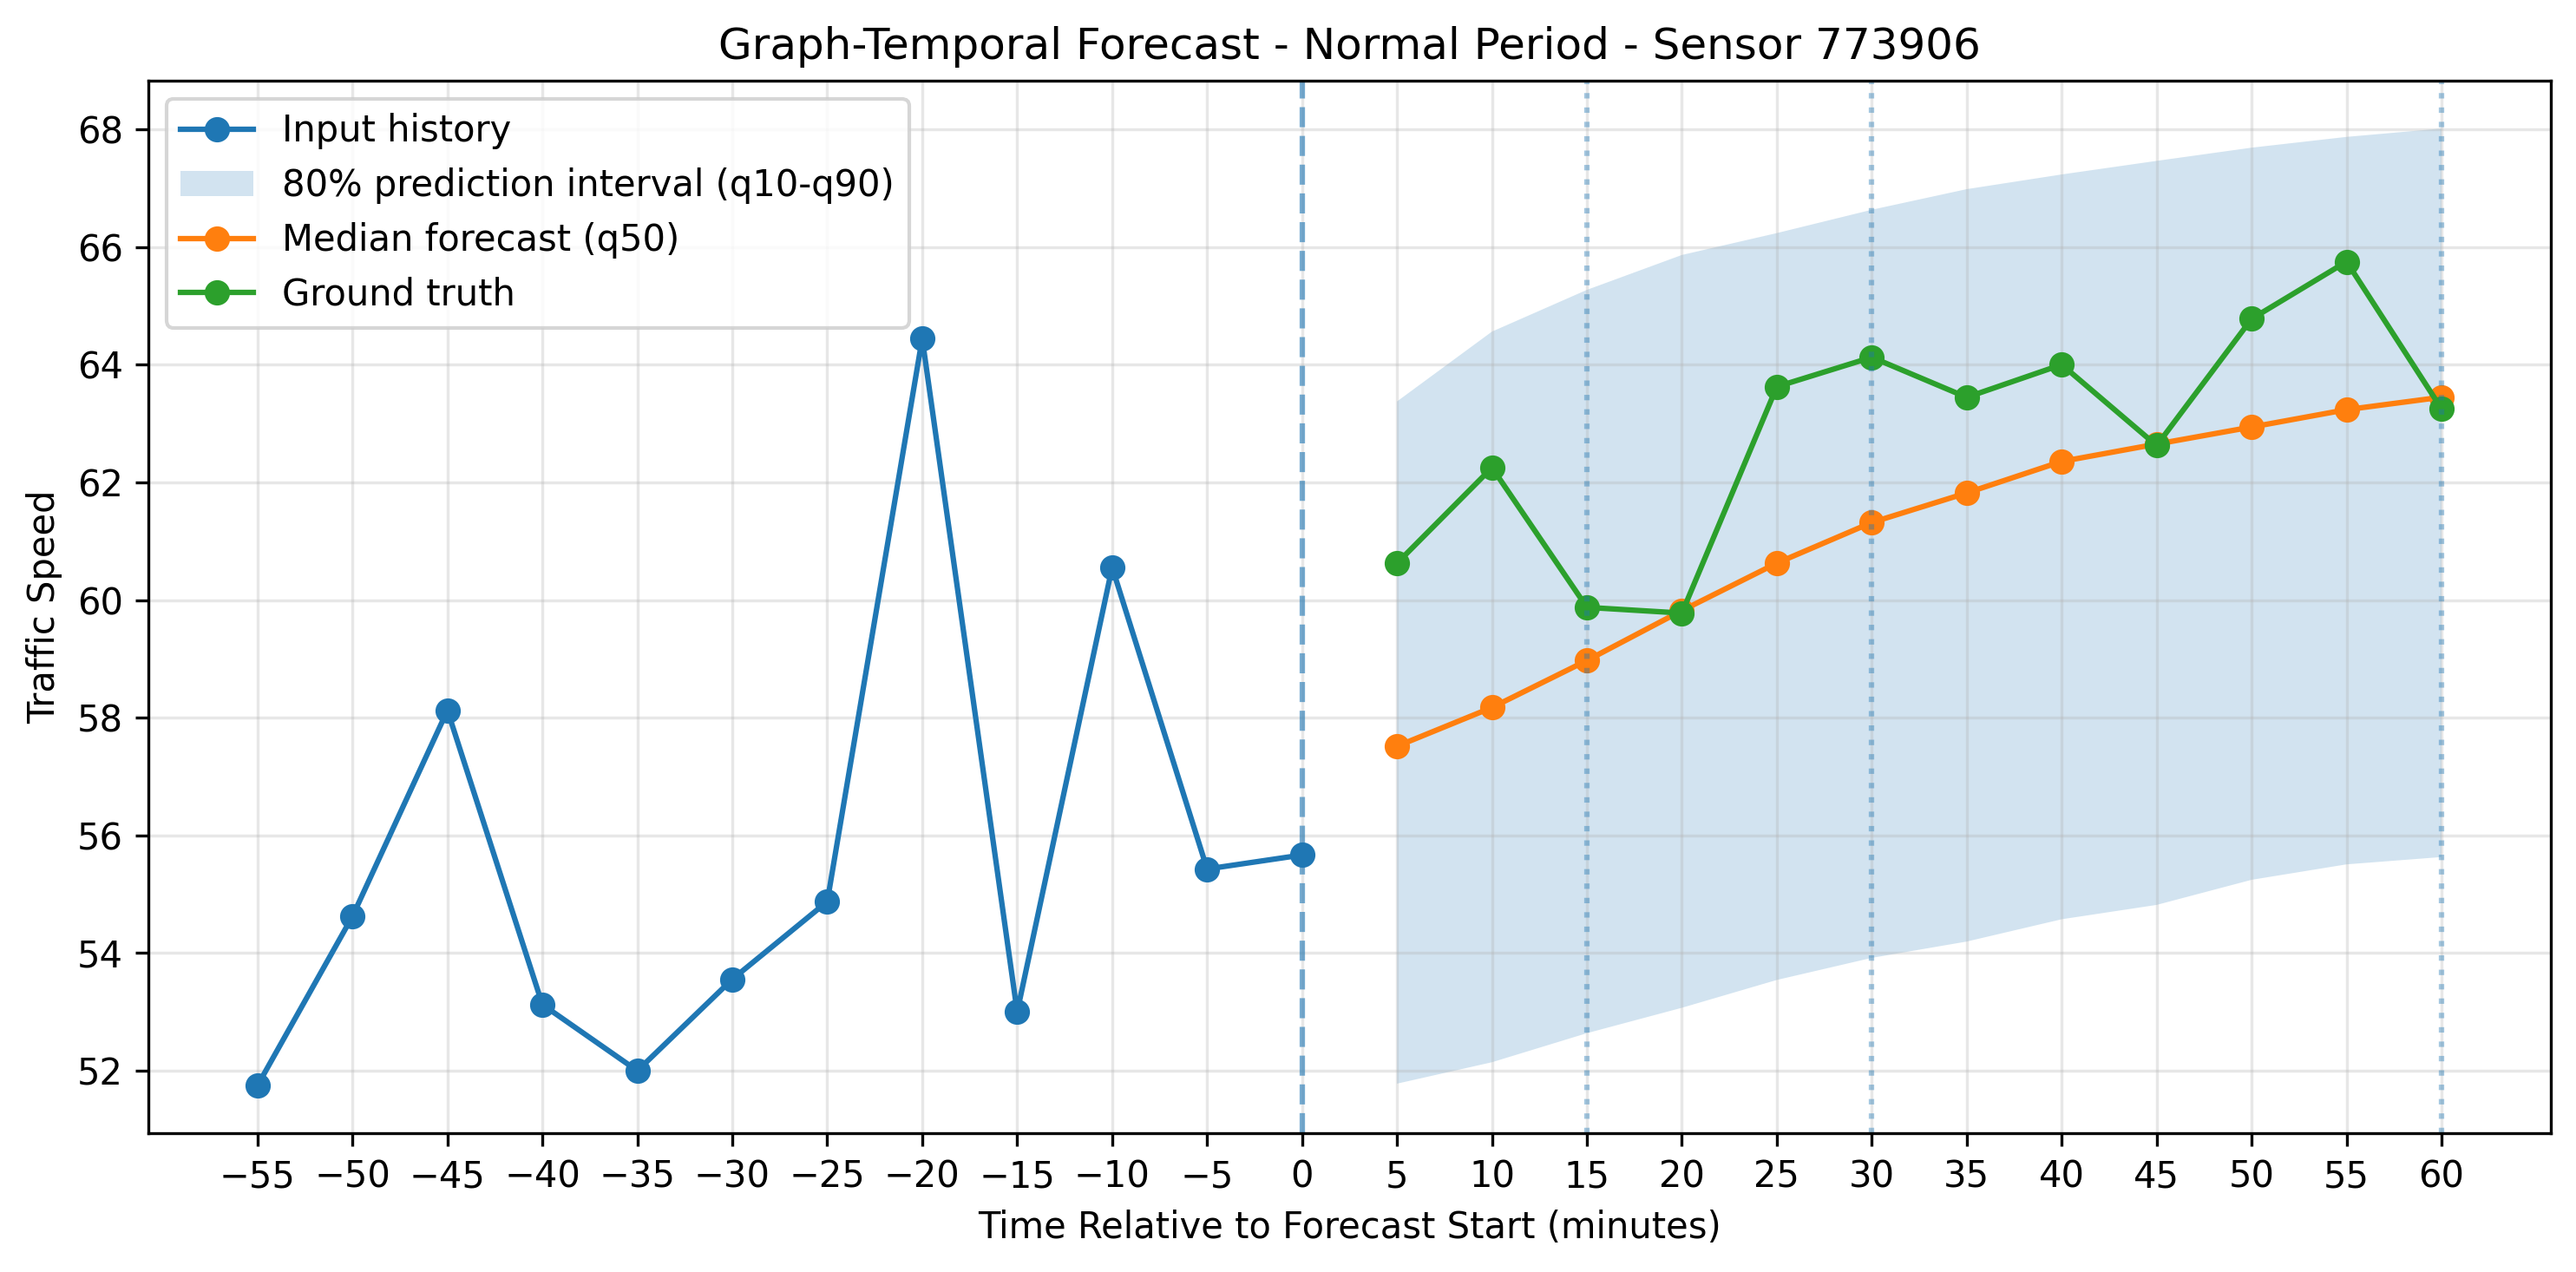
\includegraphics[width=\linewidth]
        {img/distribution_shift/normal_period}
    \end{minipage}
    \hfill
    \begin{minipage}[b]{0.49\linewidth}
        \centering
        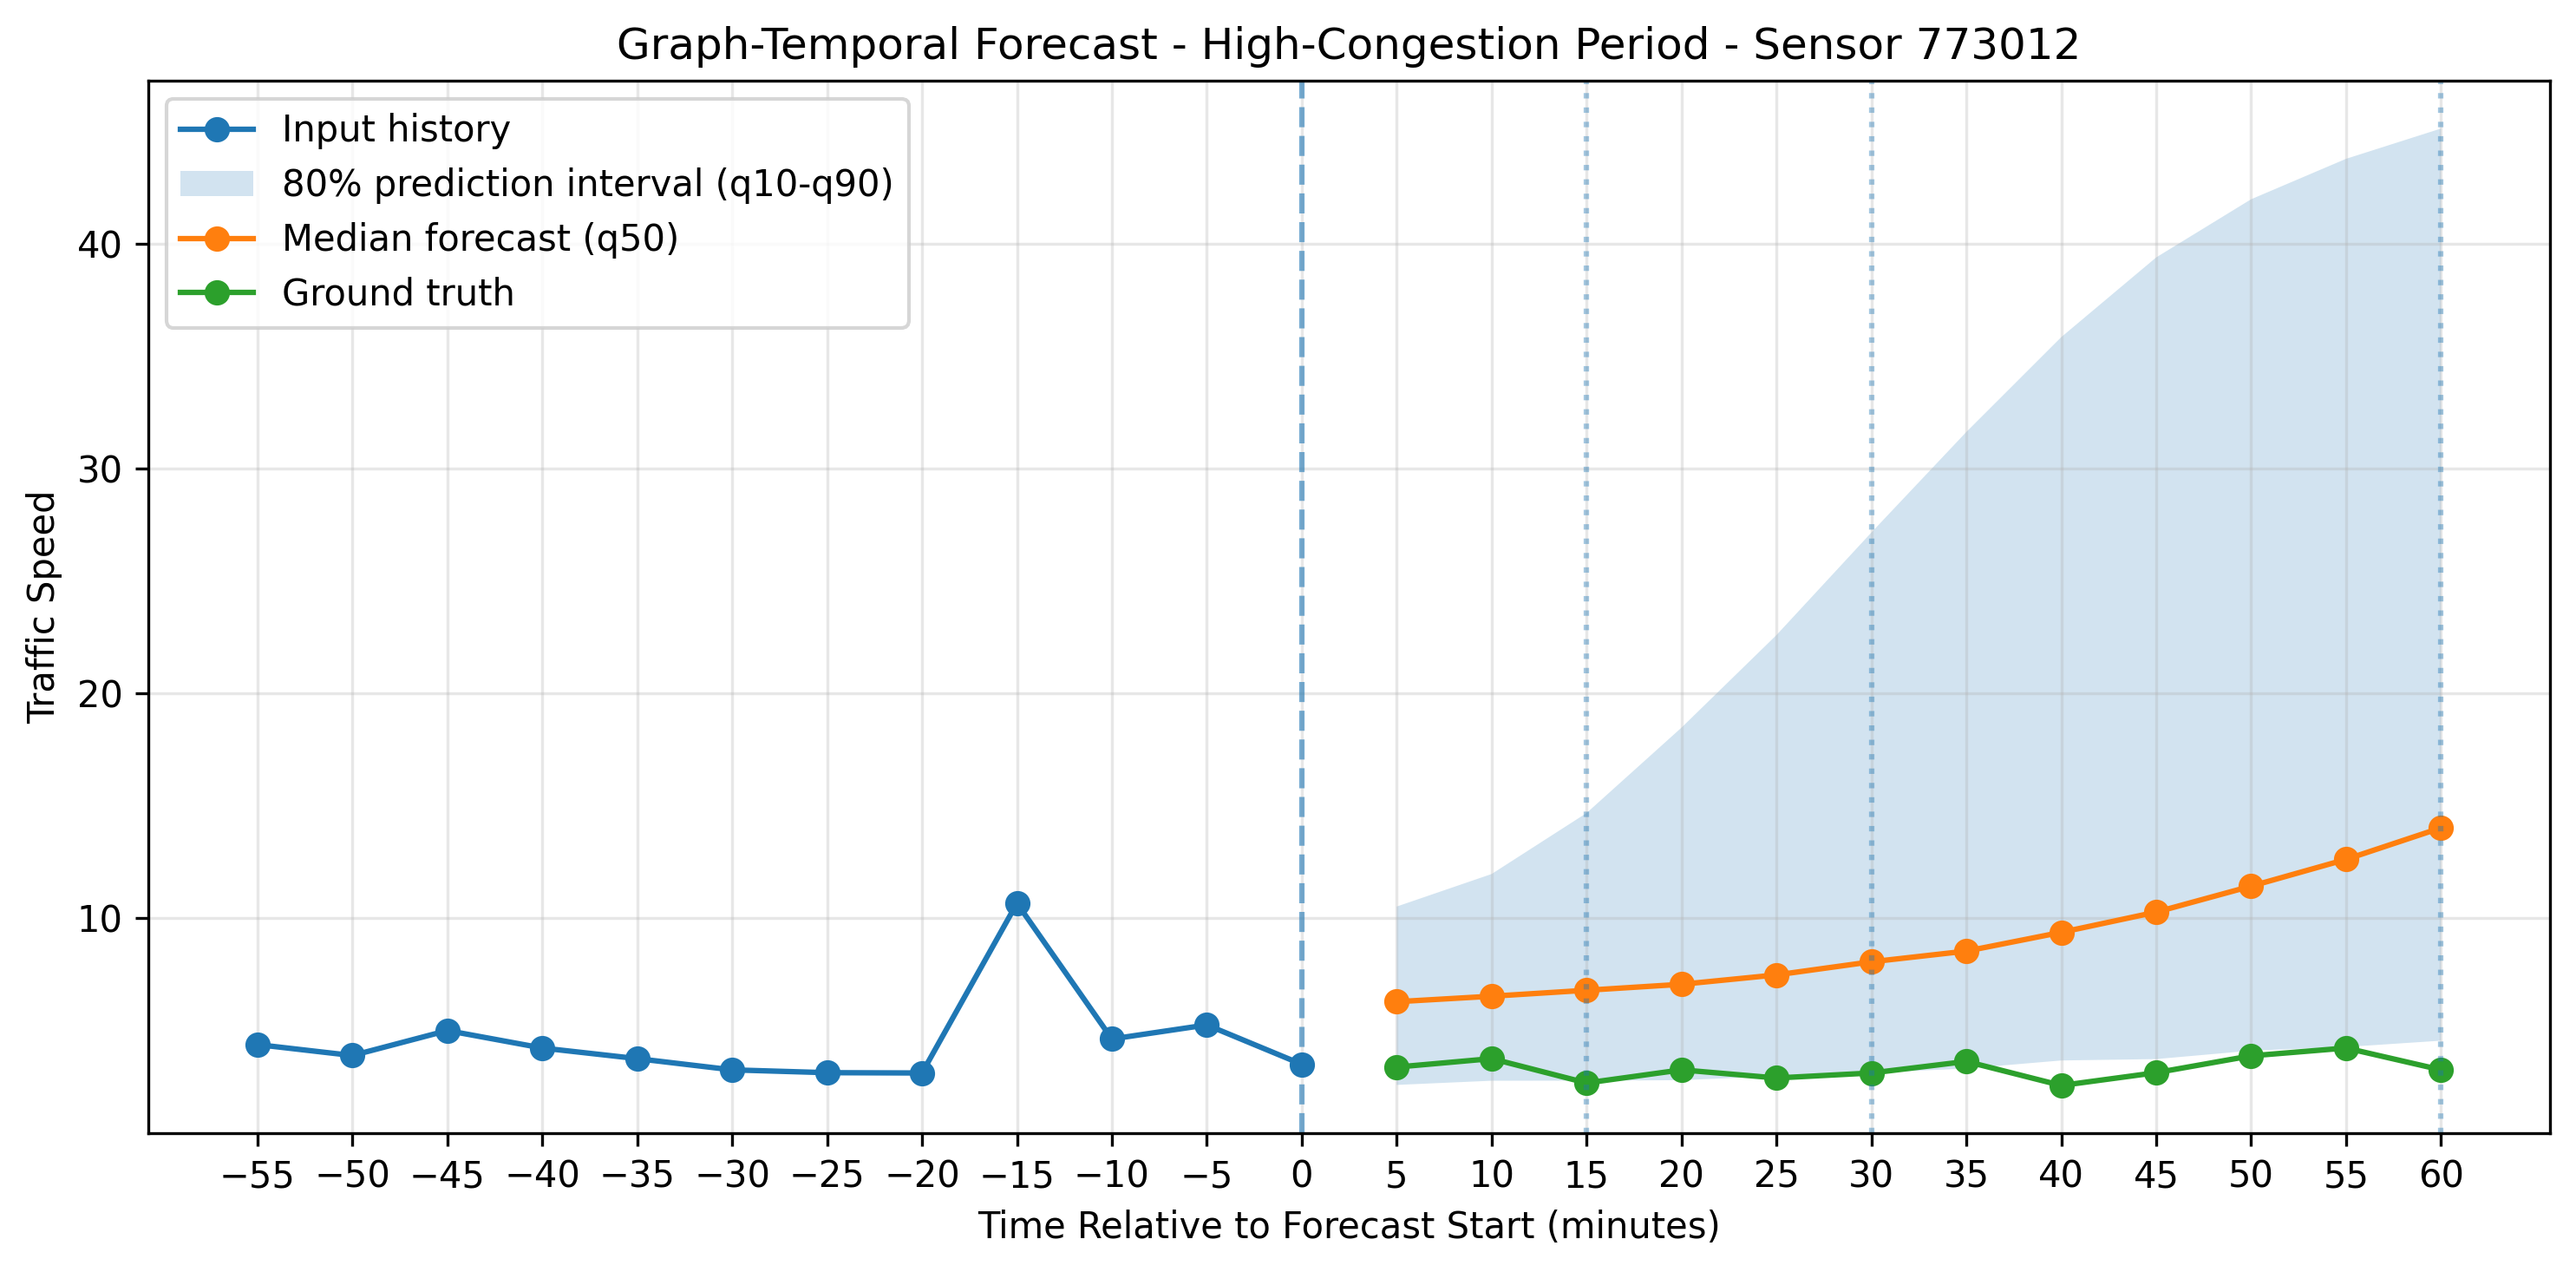
\includegraphics[width=\linewidth]
        {img/distribution_shift/high_congestion_period}
    \end{minipage}

    \caption{Representative probabilistic forecasts produced by the
    Graph-Temporal model under normal (left) and high-congestion (right)
    conditions.}
    \label{fig:shift_examples}
\end{figure}

Figure~\ref{fig:shift_examples} provides a qualitative view of how the
forecasting behavior changes between normal and high-congestion conditions.
In the normal example (left), traffic speeds remain relatively high and the
model successfully captures the increasing trend observed over the forecasting
window. Although the median forecast does not reproduce every short-term
fluctuation of the ground truth, it follows its overall evolution, while the
prediction interval remains moderately wide and contains the observed values
throughout most of the horizon.

A markedly different behavior emerges in the high-congestion example (right).
The very low observed speeds reflect a strongly congested traffic regime.
The median forecast remains relatively close to the ground truth at the
beginning of the forecasting window, but progressively overestimates future
traffic speed as the horizon increases. At the same time, the prediction
interval is substantially wider than in the normal example and expands
further toward longer horizons. This widening indicates that the model
recognizes the increasing uncertainty associated with forecasting the
evolution of the congested state. Nevertheless, the ground-truth values
remain below the lower prediction bound for most of the forecasting window.
Therefore, even though the model expresses considerably greater uncertainty,
the predictive interval is not sufficiently well positioned to cover the
actual traffic evolution.

These examples illustrate the two effects identified quantitatively in
Section~\ref{subsec:shift_quantitative}. High congestion increases the
difficulty of the point forecasting task and simultaneously leads the model
to produce wider uncertainty intervals. However, increasing interval width
alone is not sufficient to guarantee reliable uncertainty estimates when the
predictive distribution is systematically displaced from the observations.
This behavior provides a qualitative explanation for the reduced empirical
coverage observed under high congestion, particularly at longer forecasting
horizons.
%\section{Mitigation Strategies}
\label{sec:mitigation}

The distribution-shift analysis showed that the Graph-Temporal model
increases the width of its prediction intervals during high-congestion
periods, but this adaptation is not sufficient to preserve the desired
coverage, particularly at the 60-minute forecasting horizon. This section
investigates a post-hoc calibration strategy designed to improve the
reliability of the probabilistic forecasts without retraining the forecasting
model. A second, training-based mitigation strategy is subsequently discussed
as a possible extension.

\subsection{Conformalized Quantile Regression}
\label{subsec:cqr}

Conformalized Quantile Regression (CQR) was applied as a post-hoc calibration
procedure to the prediction intervals produced by the trained Graph-Temporal
model. The method uses the validation set as a calibration set and adjusts
the lower and upper predicted quantiles according to their observed
nonconformity with respect to the ground truth. The median prediction is left
unchanged, so the procedure affects uncertainty estimation without modifying
the point forecast.

For each valid calibration target $y_i$, with predicted lower and upper
quantiles $\hat{q}_{0.1,i}$ and $\hat{q}_{0.9,i}$, the nonconformity score is
defined as

\begin{equation}
    s_i =
    \max\left(
        \hat{q}_{0.1,i} - y_i,\,
        y_i - \hat{q}_{0.9,i}
    \right).
    \label{eq:cqr_score}
\end{equation}

The score measures how far an observation lies outside the predicted
interval. Observations already contained within the interval produce
non-positive scores, whereas positive scores quantify the amount by which
the interval fails to cover the target.

The calibration scores are then used to determine how much the original
prediction intervals should be enlarged. Since the target coverage is 80\%,
the desired miscoverage level is $\alpha=0.2$. Let $n_{\mathrm{cal}}$ denote
the number of valid calibration scores. The correction $\hat{s}$ is selected
as the empirical quantile of the calibration scores at level

\begin{equation}
    q =
    \frac{\left\lceil (n_{\mathrm{cal}}+1)(1-\alpha) \right\rceil}
         {n_{\mathrm{cal}}},
    \label{eq:cqr_quantile_level}
\end{equation}

and therefore

\begin{equation}
    \hat{s}
    =
    Q_q\left(\{s_i\}_{i=1}^{n_{\mathrm{cal}}}\right).
    \label{eq:cqr_correction}
\end{equation}

Intuitively, $\hat{s}$ represents the amount by which the original interval
must be expanded so that approximately 80\% of the calibration targets are
covered.

The calibrated prediction interval for a test observation is obtained by
expanding both bounds by this correction,

\begin{equation}
    \left[
        \hat{q}_{0.1,i} - \hat{s},
        \;
        \hat{q}_{0.9,i} + \hat{s}
    \right].
    \label{eq:cqr_interval}
\end{equation}

The procedure is performed separately for each forecasting horizon, allowing
the calibration correction to reflect the different uncertainty levels at
15, 30, and 60 minutes. All calibration quantities are estimated exclusively
from the validation partition and are subsequently kept fixed during test
evaluation. Therefore, no test targets are used to determine the conformal
correction.

CQR therefore provides a lightweight mitigation strategy: it does not alter
the Graph-Temporal architecture, its learned parameters, or its median
forecast, but only recalibrates the predicted uncertainty intervals. This
makes it particularly suitable for the failure mode identified in
Section~\ref{sec:distribution_shift}, where the model already reacts to
high-congestion conditions by increasing interval width, but still exhibits
residual undercoverage.


\subsubsection{Calibration Results}
\label{subsubsec:cqr_results}

The effect of CQR is evaluated by comparing the empirical coverage and
prediction interval width before and after calibration. Table~\ref{tab:cqr_results}
reports the results for the complete test set and separately for normal and
high-congestion conditions.

\begin{table}[t]
    \centering
    \caption{Empirical coverage before and after CQR calibration under
    overall, normal, and high-congestion test conditions.}
    \label{tab:cqr_results}
    \begin{tabular}{llrr}
        \toprule
        Condition & Horizon & Before CQR (\%) & After CQR (\%) \\
        \midrule
        Overall
        & 15 min & 78.44 & 80.24 \\
        & 30 min & 78.22 & 80.14 \\
        & 60 min & 78.13 & 79.96 \\
        \midrule
        Normal
        & 15 min & 78.4 & 80.27 \\
        & 30 min & 78.3 & 80.23 \\
        & 60 min & 78.3 & 80.21 \\
        \midrule
        High congestion
        & 15 min & 78.74 & 79.89 \\
        & 30 min & 77.87 & 79.07 \\
        & 60 min & 75.81 & 77.04 \\
        \bottomrule
    \end{tabular}
\end{table}

As shown in Table~\ref{tab:cqr_results}, CQR effectively corrects the mild
undercoverage observed on the complete test distribution. Empirical coverage
increases from 78.44\%, 78.22\%, and 78.13\% to 80.24\%, 80.14\%, and
79.96\% at the 15, 30, and 60-minute horizons, respectively. The calibrated
intervals are therefore very close to the nominal 80\% coverage level across
all three forecasting horizons.

A similar behavior is observed under normal traffic conditions, where
coverage after calibration reaches 80.27\%, 80.23\%, and 80.21\%. This is
consistent with the fact that normal conditions represent the dominant
operating regime in both the calibration and test distributions. CQR is
therefore effective at correcting the systematic in-distribution
miscalibration of the original prediction intervals.

The improvement is more limited under high congestion. Coverage increases
from 78.74\% to 79.89\% at 15 minutes and from 77.87\% to 79.07\% at
30 minutes, bringing both substantially closer to the nominal level. At
60 minutes, however, coverage increases only from 75.81\% to 77.04\% and
remains clearly below the desired 80\%. Thus, the same calibration procedure
that provides nearly nominal coverage overall does not fully correct the
undercoverage observed in the most challenging shifted condition.


\begin{figure}[t]
    \centering

    \begin{minipage}[b]{0.49\linewidth}
        \centering
        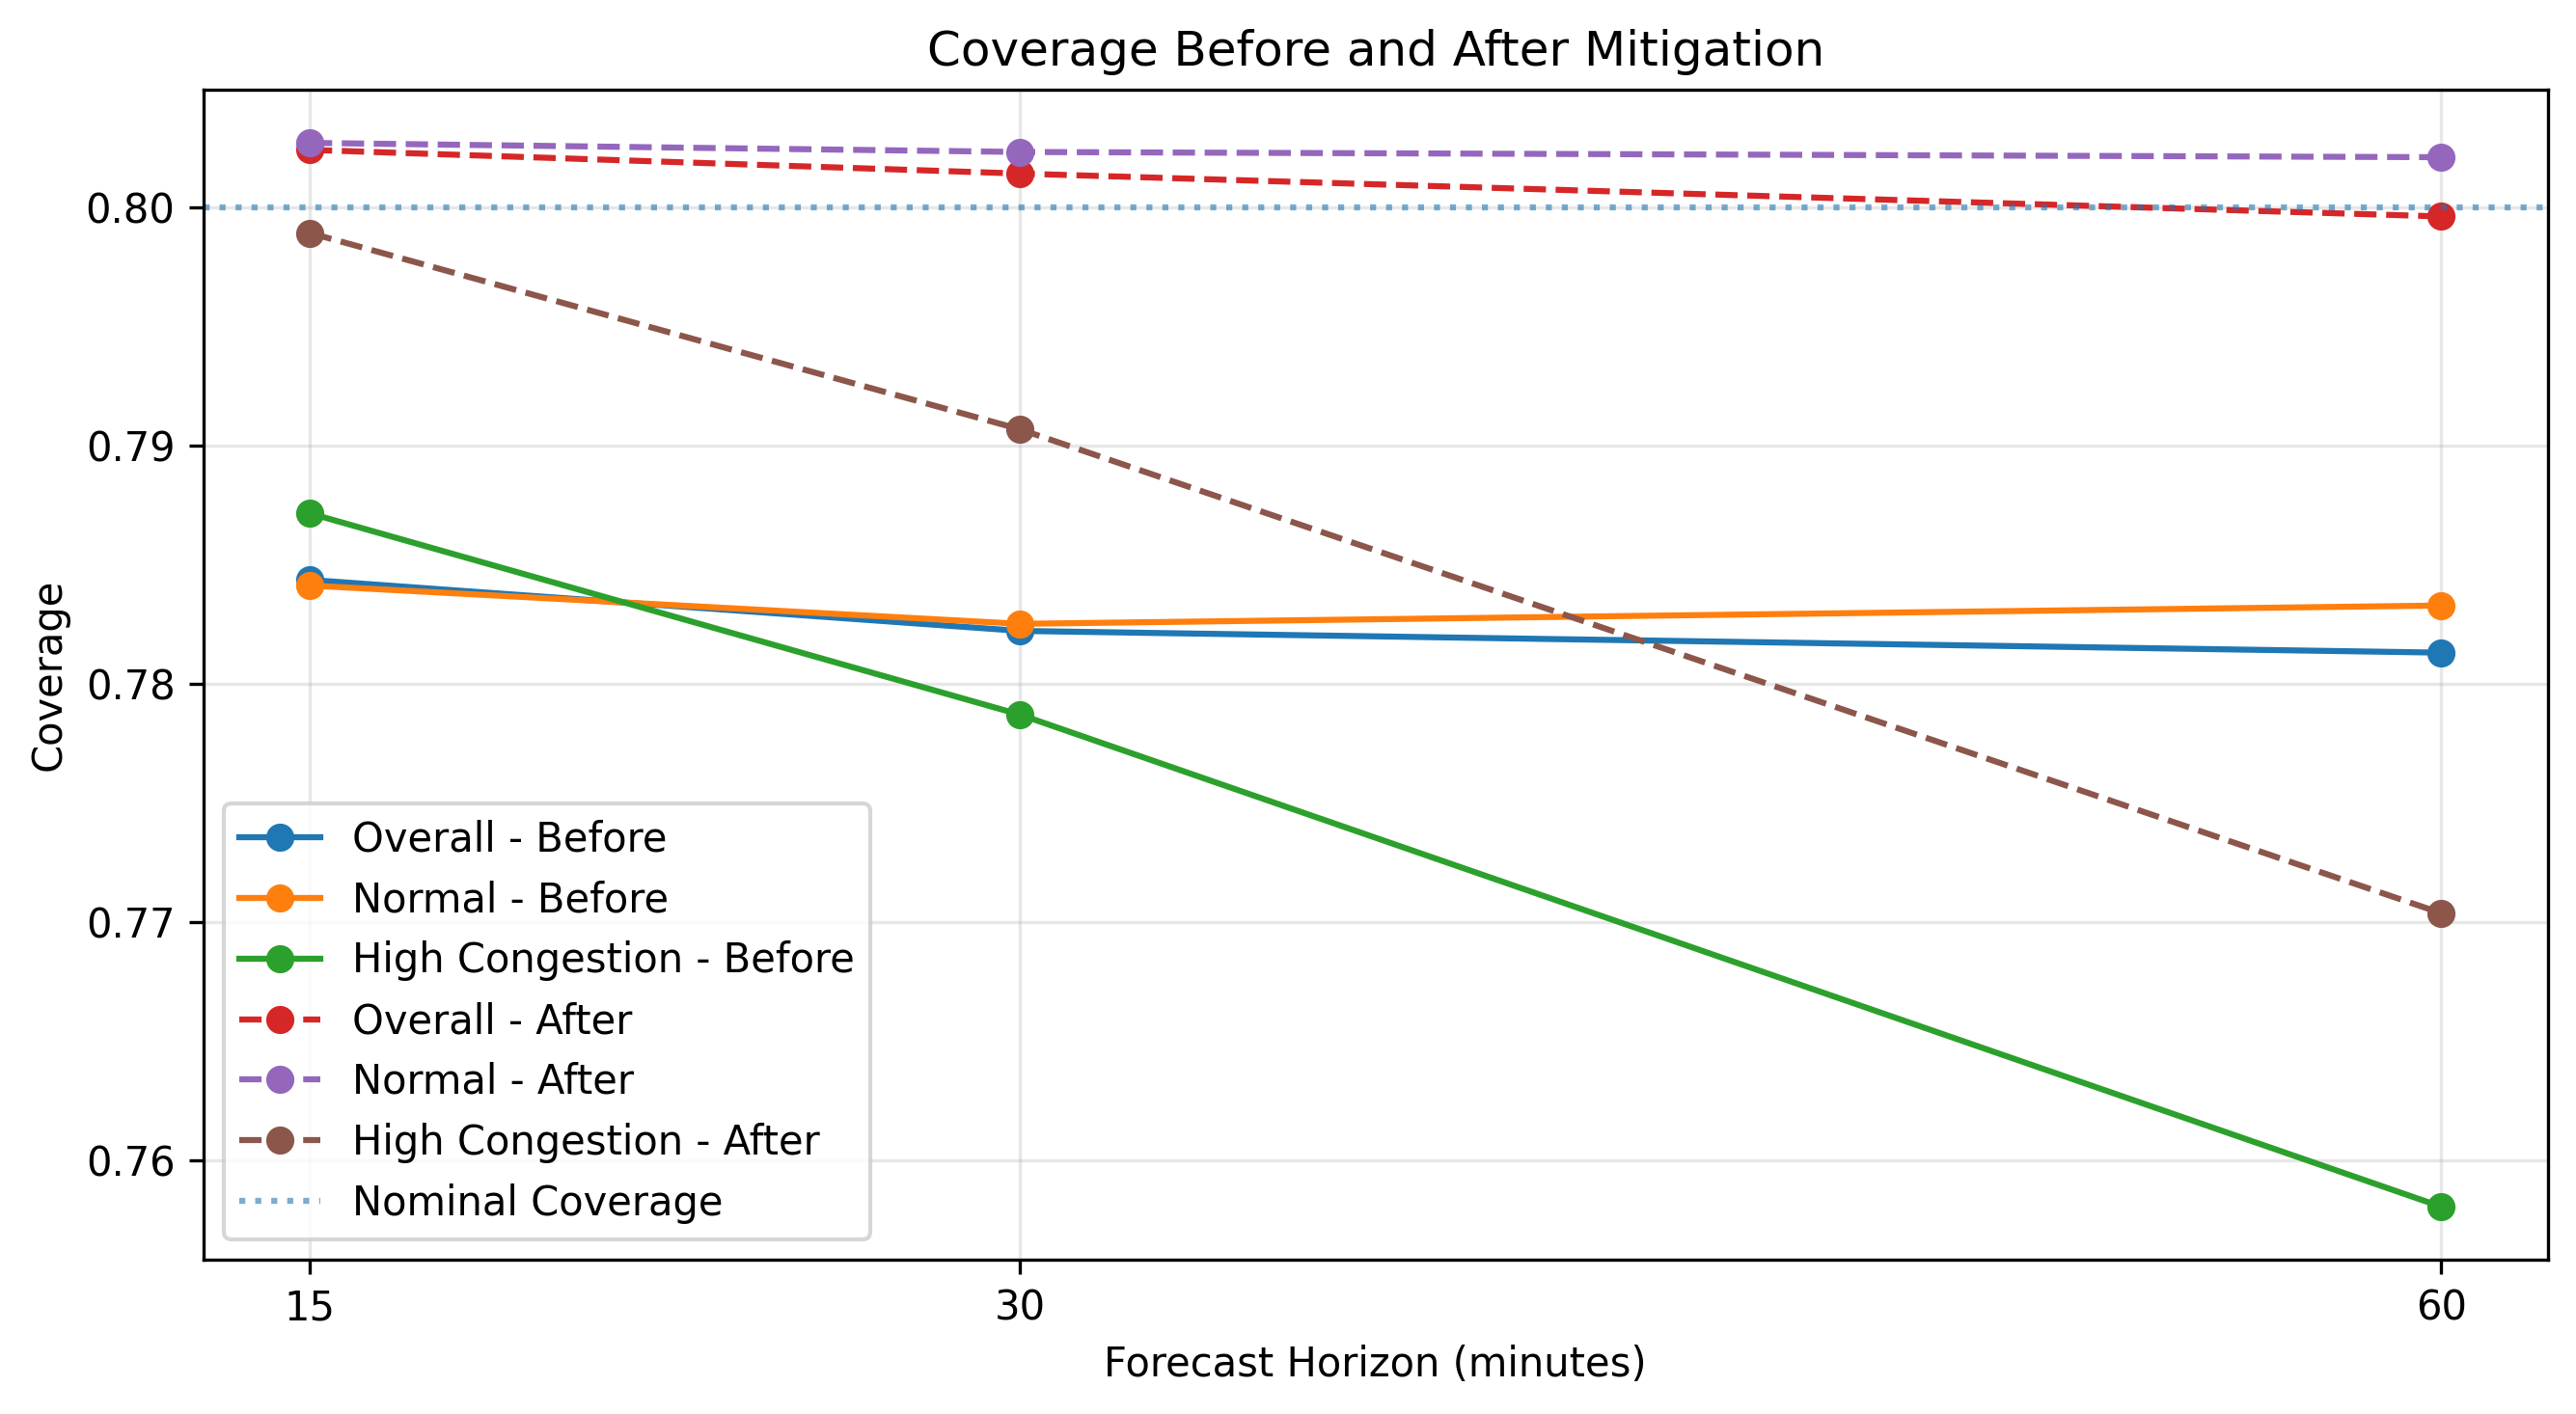
\includegraphics[width=\linewidth]{img/mitigation_strategy/coverage_mitigation_comparison}
    \end{minipage}
    \hfill
    \begin{minipage}[b]{0.49\linewidth}
        \centering
        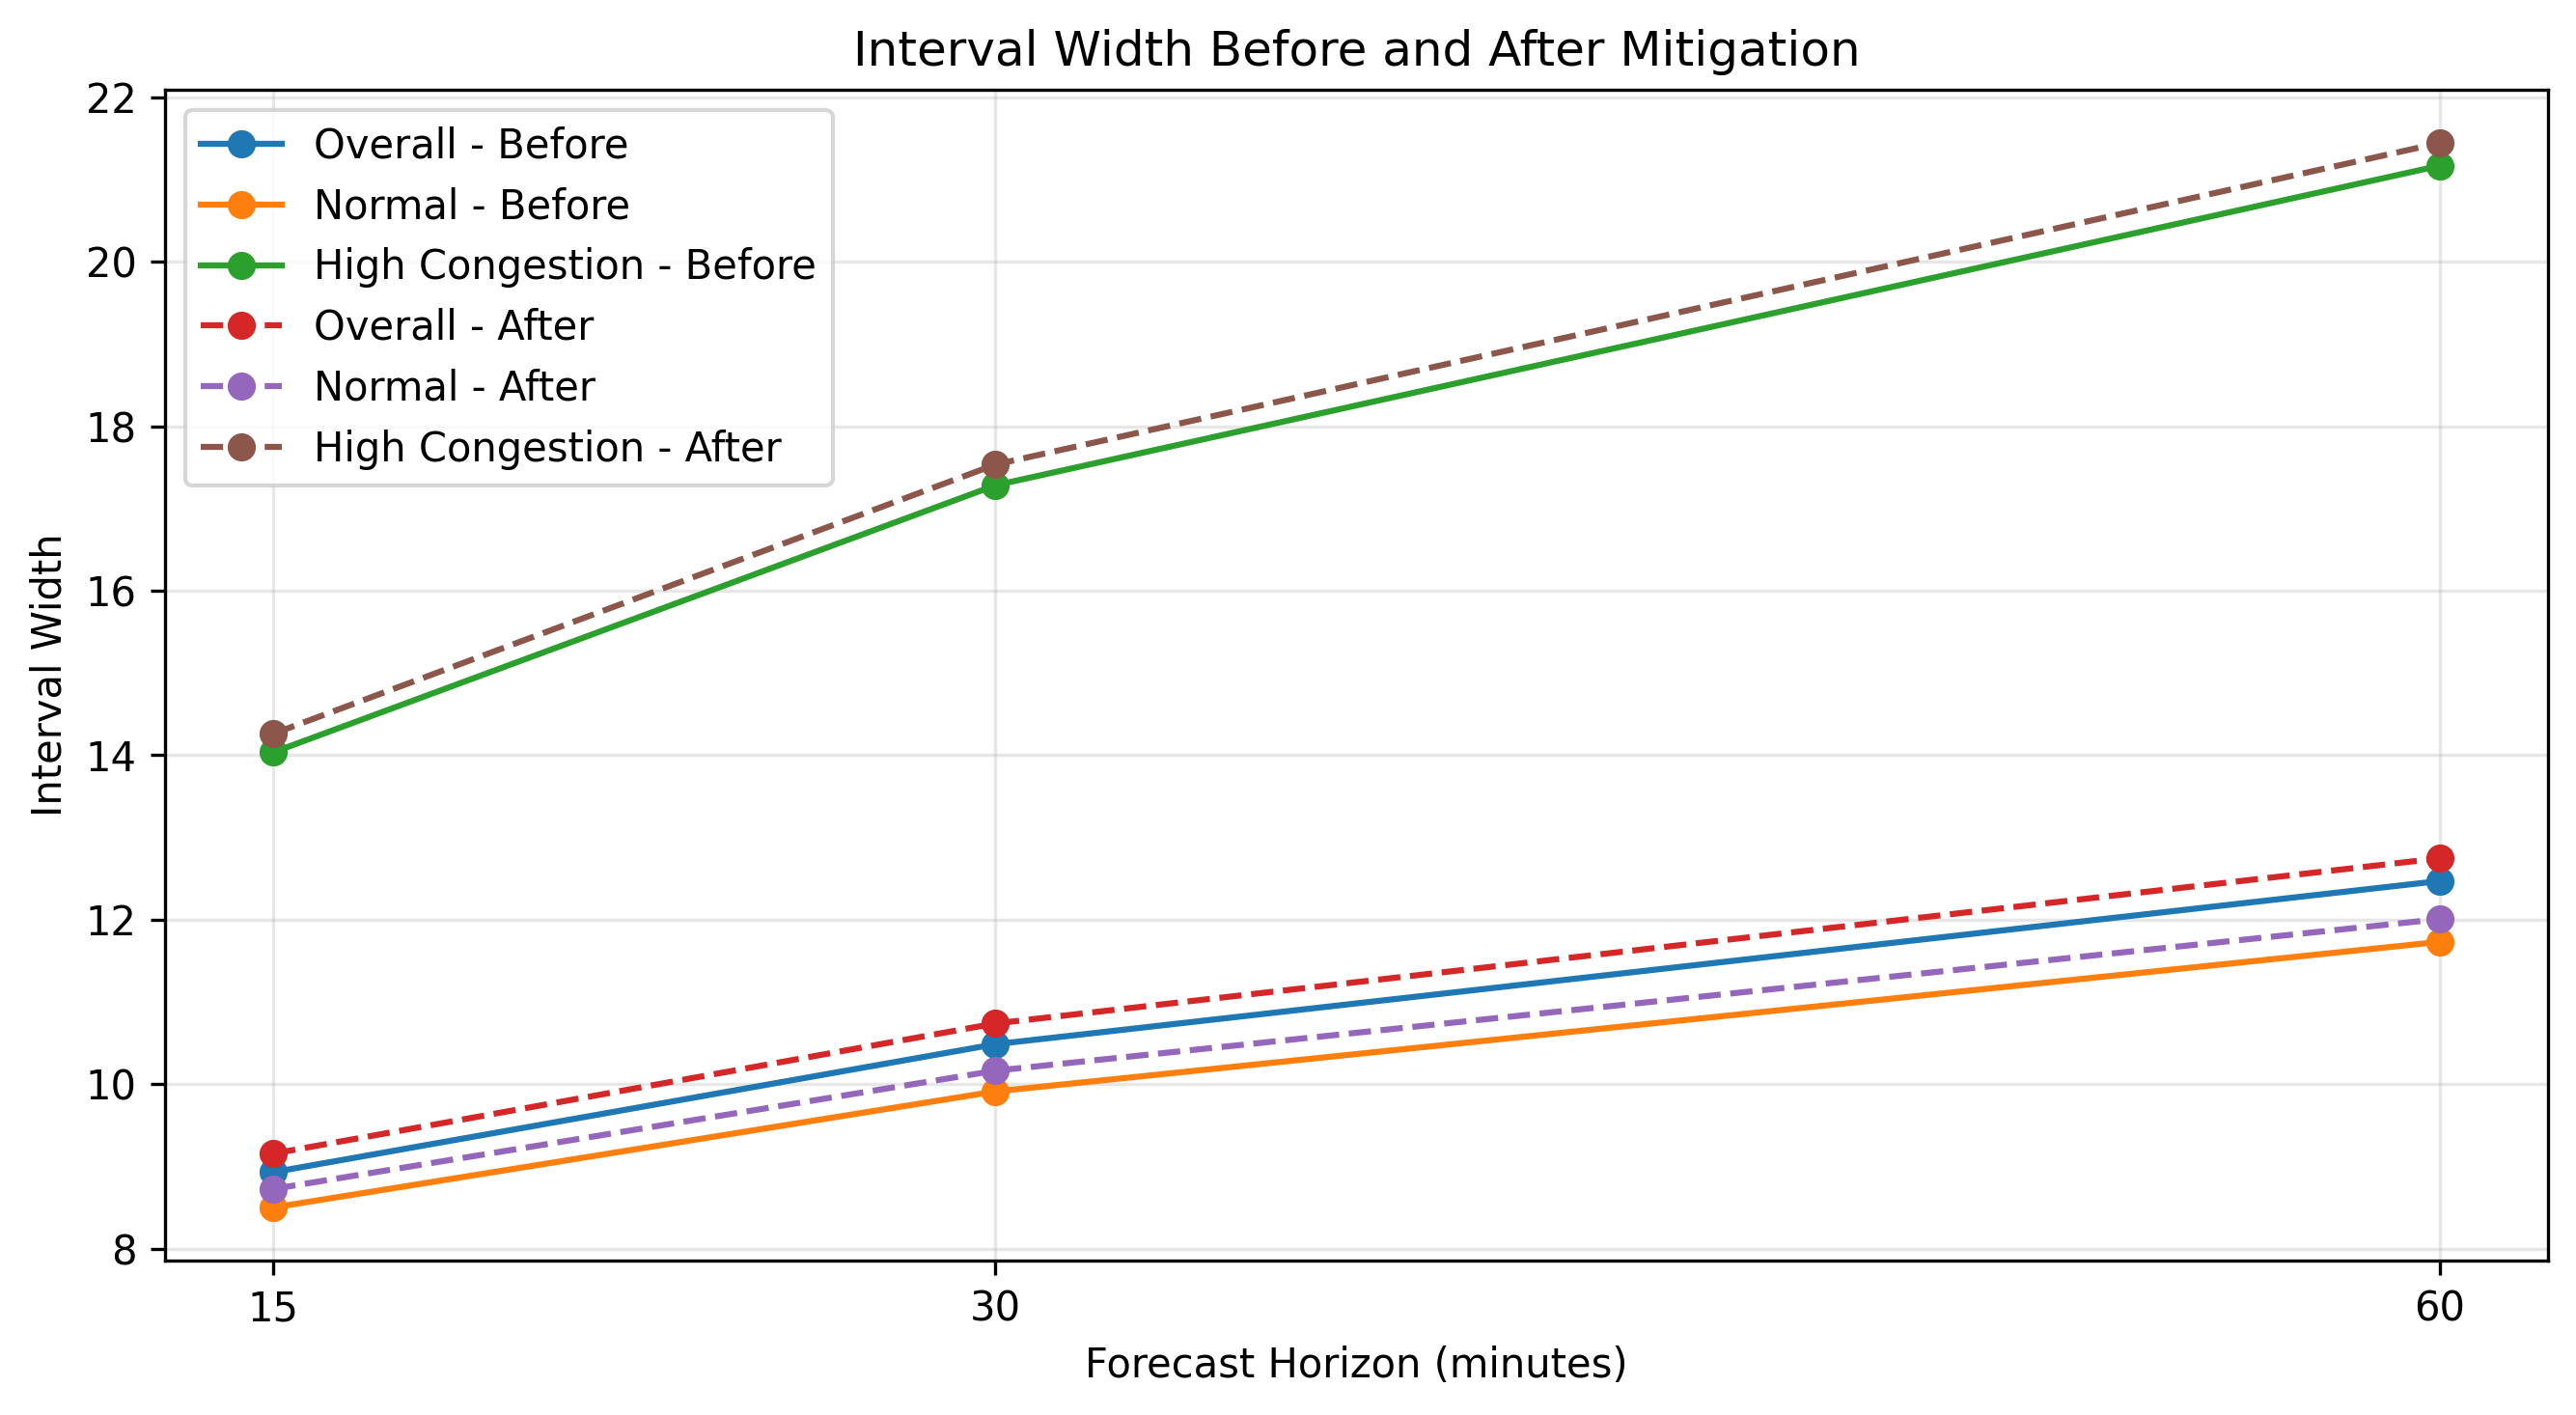
\includegraphics[width=\linewidth]{img/mitigation_strategy/interval_width_mitigation_comparison}
    \end{minipage}

    \caption{Effect of CQR calibration on empirical coverage (left) and
    prediction interval width (right) under overall, normal, and
    high-congestion conditions.}
    \label{fig:cqr_results}
\end{figure}

Figure~\ref{fig:cqr_results} shows that the improvement in coverage is
obtained by moderately expanding the original prediction intervals. Since
CQR leaves the median forecast unchanged, this calibration step improves
uncertainty reliability without altering point forecasting accuracy.

The remaining gap under high congestion, particularly at 60 minutes,
highlights an important limitation of the global calibration strategy.

Overall, CQR successfully mitigates the general undercoverage of the
Graph-Temporal model and substantially improves calibration under normal
conditions. It also improves coverage during high congestion, but does not
completely eliminate the reliability degradation observed at the longest
forecasting horizon. This residual failure motivates considering mitigation
strategies that explicitly account for congestion during model training.


\subsection{Congestion-Aware Training}
\label{subsec:congestion_aware}

Although CQR improves the calibration of the prediction intervals, the
remaining undercoverage under high-congestion conditions suggests that a
global post-hoc correction cannot completely address the distribution shift.
A complementary mitigation strategy would therefore intervene directly
during model training, encouraging the model to allocate greater importance
to observations belonging to congested traffic regimes.

A possible approach is to introduce a congestion-aware weighted version of
the masked Pinball Loss. The congestion condition can be defined using the
same training-derived criterion introduced in
Section~\ref{subsec:congestion_definition}. In particular, each target
timestamp can be associated with its congestion ratio $C_t$, computed using
the per-sensor thresholds estimated exclusively from the training data.

The standard masked Pinball Loss can then be modified by assigning a larger
weight to targets associated with high-congestion conditions. Let
$w_{b,h}$ denote the weight associated with forecasting horizon $h$ of sample
$b$. A simple weighting scheme is

\begin{equation}
    w_{b,h} =
    \begin{cases}
        1 + \lambda, & \text{if } C_{t_b+h} \geq \tau_{\mathrm{peak}}, \\
        1,           & \text{otherwise},
    \end{cases}
    \label{eq:congestion_weight}
\end{equation}

where $\lambda \geq 0$ controls the additional importance assigned to
high-congestion targets. The resulting weighted objective becomes

\begin{equation}
    \mathcal{L}_{\mathrm{weighted}}
    =
    \frac{
        \displaystyle
        \sum_b \sum_h \sum_n
        w_{b,h}\,m_{b,h,n}
        \sum_{q \in \mathcal{Q}}
        \mathcal{L}_q
        \left(
            y_{b,h,n},
            \hat{y}^{(q)}_{b,h,n}
        \right)
    }{
        \displaystyle
        |\mathcal{Q}|
        \sum_b \sum_h \sum_n
        w_{b,h}\,m_{b,h,n}
    }.
    \label{eq:weighted_pinball}
\end{equation}

This modification increases the contribution of congested targets to the
training objective without discarding or undersampling observations from
normal traffic conditions. The hyperparameter $\lambda$ would control the
strength of the reweighting and should be selected using the validation set,
considering both normal and high-congestion performance.

Unlike CQR, which adjusts already estimated prediction intervals, this
strategy would modify the parameters learned by the forecasting model.
Consequently, it could potentially improve both the median forecast and the
estimated conditional quantiles during congestion. This is particularly
relevant to the qualitative behavior observed in
Figure~\ref{fig:shift_examples}, where the high-congestion example exhibits
not only insufficient interval coverage but also a progressively displaced
median forecast at longer horizons.

Importantly, the congestion labels would only be required during training
to construct the weights in Equation~\ref{eq:congestion_weight}. At inference
time, the trained model would continue to receive exactly the same inputs as
the original Graph-Temporal model and would not require knowledge of future
congestion conditions.

This approach was not implemented in the present work and is therefore
proposed as a possible extension rather than evaluated experimentally.
Compared with the post-hoc CQR mitigation, congestion-aware training directly
targets the regime in which the largest degradation was observed. However,
increasing the contribution of relatively rare congestion events may introduce
a trade-off with performance under normal conditions. For this reason, the
weighting strength should be selected carefully and evaluated separately on
normal and high-congestion subsets.

The two mitigation strategies therefore operate at different stages of the
forecasting pipeline. CQR provides a lightweight post-hoc correction that
successfully improves marginal calibration without retraining the model,
whereas congestion-aware training could potentially address the underlying
conditional forecasting errors by explicitly exposing the optimization
objective to the importance of rare congestion regimes.
%\section{Computational Cost and Accuracy-Reliability Trade-off}
\label{sec:cost_tradeoff}

The introduction of graph-based message passing improves forecasting accuracy,
but also increases model complexity and computational cost.
Table~\ref{tab:computational_cost} compares the Temporal model and the selected
Graph-Temporal model in terms of number of trainable parameters and training
time.

\begin{table}[t]
    \centering
    \caption{Computational cost of the Temporal and Graph-Temporal models.}
    \label{tab:computational_cost}
    \begin{tabular}{lrr}
        \toprule
        Model & Trainable Parameters & Training Time (min) \\
        \midrule
        Temporal GRU   & 40164 & 14.3 \\
        Graph-Temporal & 64868 & 34.0 \\
        \bottomrule
    \end{tabular}
\end{table}

As shown in Table~\ref{tab:computational_cost}, the Graph-Temporal model
contains 64868 trainable parameters compared with 40164 for the Temporal
model, corresponding to an increase of approximately 61.5\%. Training time also
increases from approximately 14.3 to 34.0 minutes, making the Graph-Temporal
model about 2.4 times more expensive to train in the considered experimental
setting. This additional cost results from the diffusion operations and from
the stacked graph-temporal blocks used to combine spatial and temporal
information.

The additional computational cost is accompanied by improved forecasting
accuracy. As shown in Section~\ref{sec:in_distribution_results}, the
Graph-Temporal model consistently outperforms the Temporal model in terms of
MAE, RMSE, and Pinball Loss, with the improvement in point forecasting
becoming more pronounced at longer horizons. It also produces sharper
prediction intervals, although with slightly lower empirical coverage.
Therefore, the accuracy gains provided by graph message passing come at the
cost of both increased computation and mild undercoverage.

Moreover, the stress-test analysis shows that this reliability gap becomes
more important under high congestion. Although the Graph-Temporal model
responds to difficult traffic conditions by producing wider intervals,
coverage decreases to 75.8\% at the 60-minute horizon. The model therefore
does not fully translate its increased uncertainty into reliable coverage
under distribution shift.

The CQR mitigation partially addresses this trade-off without increasing
model complexity or requiring retraining. Post-hoc calibration brings overall
coverage close to the nominal 80\% level while leaving the median point
forecast unchanged. Nevertheless, the remaining undercoverage under
high-congestion conditions shows that improved average calibration does not
necessarily imply equally reliable uncertainty estimates across different
traffic regimes.

Overall, the Graph-Temporal architecture provides a clear accuracy advantage
over the purely temporal baseline at the cost of greater computational
complexity. Its probabilistic forecasts are generally sharper and more
accurate in terms of quantile loss, but require additional calibration to
approach the desired coverage. The results therefore highlight that model
selection should consider not only point forecasting accuracy, but also
computational cost and the reliability of predictive uncertainty,
particularly under distribution shift.


%\section{Discussion}
\label{sec:discussion}

\subsection{Main Findings}
\label{subsec:main_findings}

The experiments provide evidence that both temporal and spatial information
are relevant for traffic forecasting on METR-LA. The Temporal model already
provides a substantial improvement over persistence, showing that recent
sensor histories contain strong predictive information. Incorporating graph
message passing further improves forecasting accuracy, with the benefit
becoming more evident at longer forecasting horizons. Moreover, the
sensor-level analysis shows that this improvement is widespread across the
network, although a small number of sensors do not benefit from spatial
information.

The graph ablations further show that the way spatial information is
represented matters. Increasing the diffusion depth from $K=2$ to $K=3$
provides only limited additional benefits and introduces a less favorable
balance between error metrics, calibration, and computational cost. In
contrast, replacing the weighted adjacency matrix with a binary one produces
a clearer degradation in forecasting accuracy, particularly at longer
horizons. This suggests that the original edge weights provide useful
information beyond graph connectivity alone.

The probabilistic analysis reveals a different aspect of model performance.
The Graph-Temporal model produces sharper intervals and lower quantile losses
than the Temporal model, but its empirical coverage is slightly below the
nominal 80\% level. More importantly, this reliability degradation becomes
stronger under distribution shift. During high-congestion periods, both point
forecasting errors and prediction interval widths increase, while coverage
decreases at longer horizons. The model therefore recognizes part of the
increased uncertainty associated with congestion, but does not fully capture
the shifted predictive distribution.

Finally, the mitigation experiments show that post-hoc calibration can
substantially improve uncertainty reliability. CQR brings overall empirical
coverage close to the nominal level without modifying the median forecasts or
retraining the model. However, residual undercoverage remains under
high-congestion conditions, particularly at the longest horizon. This result
indicates that good marginal calibration does not necessarily imply equally
reliable uncertainty estimates under specific shifted conditions and
motivates mitigation strategies that explicitly account for rare traffic
regimes during training.


\subsection{Limitations}
\label{subsec:limitations}

Several limitations should be considered when interpreting the results.
First, the experiments are conducted exclusively on METR-LA and therefore
reflect the spatial structure, traffic dynamics, and missing-data patterns of
a single road network. The conclusions cannot necessarily be generalized to
other cities or sensor networks without additional evaluation.

Second, the definition of distribution shift considered in this work focuses
specifically on high-congestion periods. Although this represents a relevant
and challenging traffic regime, other forms of shift may affect forecasting
models differently, including sensor failures, changes in network topology,
or temporal changes in traffic patterns.

Third, the Graph-Temporal architecture is intentionally compact and explores
only a limited set of spatial configurations. The diffusion-depth and
adjacency ablations provide evidence about the role of graph information, but
they do not constitute an exhaustive exploration of graph neural network
architectures or graph construction strategies.

Finally, CQR is calibrated globally for each forecasting horizon using the
validation distribution. While this substantially improves marginal
coverage, it does not explicitly account for traffic regime and therefore
cannot guarantee the same calibration quality within the high-congestion
subset. In addition, the temporal and spatial dependence present in traffic
data makes the standard exchangeability assumptions underlying conformal
prediction less directly applicable.


\subsection{Future Improvements}
\label{subsec:future_improvements}

Several extensions could address these limitations. A first direction would
be to evaluate the proposed congestion-aware training objective, assigning
greater importance to rare congested targets during optimization and
measuring whether this improves both point forecasts and uncertainty
estimation without substantially degrading performance under normal
conditions.

The robustness analysis could also be extended to additional distribution
shifts, such as partially masked sensor histories or simulated sensor
failures. This would provide a broader characterization of the dependence of
the Graph-Temporal model on spatial information and of its behavior when
parts of the network become unavailable.

Finally, future work could explore more expressive spatial and temporal
architectures, alternative graph construction strategies, and dynamic graphs
whose relationships evolve with traffic conditions. Evaluation on additional
traffic datasets would also be necessary to determine whether the conclusions
observed on METR-LA generalize to different road networks and traffic
regimes.
%\section{Conclusion}
\label{sec:conclusion}

This work investigated probabilistic graph-based traffic forecasting under
distribution shift using the METR-LA dataset. A leakage-free experimental
pipeline was developed to compare a persistence baseline, a purely temporal
GRU, and a Graph-Temporal model combining diffusion-based message passing with
recurrent temporal modeling. In addition to point forecasting accuracy, the
analysis considered predictive uncertainty through quantile regression,
empirical coverage, and prediction interval width.

The experimental results show that incorporating the road-network graph
consistently improves forecasting accuracy over the Temporal model,
particularly at longer forecasting horizons. The graph ablations further
indicate that the weighted connectivity structure contains useful predictive
information, while increasing the diffusion depth provides only limited
additional benefits. These improvements, however, come with higher
computational cost and slightly reduced empirical coverage.

The high-congestion stress test reveals a more challenging limitation.
During congested periods, forecasting errors increase substantially and the
model responds by producing wider prediction intervals. Nevertheless,
coverage deteriorates at longer horizons, showing that increased uncertainty
does not necessarily translate into reliable uncertainty estimates under
distribution shift.

Post-hoc calibration through Conformalized Quantile Regression substantially
improves overall coverage and brings it close to the nominal 80\% level
without modifying the median forecasts or retraining the model. However, the
remaining undercoverage under high congestion shows that marginal calibration
alone is insufficient to fully address regime-specific reliability. A
congestion-aware training objective was therefore proposed as a possible
extension to explicitly increase the importance of these rare and difficult
traffic conditions during learning.

Overall, the results demonstrate the value of exploiting spatial information
for traffic forecasting while also highlighting the importance of evaluating
predictive uncertainty beyond average test performance. Reliable deployment
requires considering not only forecasting accuracy, but also calibration,
robustness to distribution shift, and the computational cost associated with
more expressive spatio-temporal models.

\section{Introduction}
\label{sec:introduction}

Accurate short-term knowledge of traffic conditions is essential for
understanding and managing the dynamics of urban road networks.
However, traffic evolution is difficult to predict because it results from
the interaction of two strongly coupled components. On the one hand, traffic
at a given location follows temporal patterns determined by its recent
history; on the other hand, changes occurring on one road segment can
propagate through the network and affect other connected locations. A
forecasting model should therefore be able to exploit both temporal
dependencies and the spatial structure of the road network.

Accurate point forecasts alone, however, are not sufficient in practical
settings. Traffic conditions may change rapidly, particularly during
congestion events, making some predictions substantially more uncertain than
others. A forecasting system should therefore provide not only an estimate of
future traffic conditions, but also an indication of the uncertainty
associated with that estimate. Moreover, this uncertainty should remain
meaningful when the model encounters conditions that differ from those
observed during training.

This work investigates these aspects using the METR-LA traffic-sensor
network. Starting from a simple persistence baseline, a temporal forecasting
model based on Gated Recurrent Units (GRUs) is first considered to model the
temporal evolution of each sensor independently. Spatial information is then
introduced through a graph-temporal architecture combining diffusion-style
message passing over the road-sensor graph with recurrent temporal modeling.
Both learned models produce probabilistic forecasts through conditional
quantile estimation, allowing point accuracy and predictive uncertainty to be
evaluated jointly.

Beyond aggregate forecasting performance, particular attention is devoted to
understanding the contribution of the graph and the robustness of the
probabilistic predictions. The graph-temporal model is analyzed at the sensor
level, under different graph configurations and diffusion depths, and under a
distribution shift defined by unusually high network-wide congestion.
Finally, calibration strategies are investigated to determine whether the
reliability of the predictive intervals can be improved when the forecasting
conditions become more challenging.


\subsection{Objectives and Research Questions}
\label{subsec:objectives}

The main objective of this work is to design and evaluate a compact,
probabilistic graph-temporal forecasting pipeline while investigating the
interaction between predictive accuracy, spatial information, uncertainty
calibration, and robustness under distribution shift.

More specifically, the experimental analysis is organized around the
following research questions:

\begin{enumerate}
    \item \textbf{Does graph message passing improve traffic forecasting
    compared with temporal modeling alone?}

    This question is investigated by comparing a persistence baseline, a
    temporal GRU without spatial information exchange, and a graph-temporal
    model that propagates information between connected traffic sensors.

    \item \textbf{How does the graph representation affect forecasting
    performance?}

    The contribution of the graph is examined both at the individual-sensor
    level and through controlled architectural experiments. In particular,
    the analysis investigates where graph message passing helps or hurts,
    whether extending the spatial diffusion depth provides additional
    benefits, and whether the original weighted graph contains useful
    information beyond connectivity alone.

    \item \textbf{How reliable are the probabilistic forecasts under normal
    and shifted traffic conditions?}

    Forecast uncertainty is evaluated through quantile-based predictive
    intervals, considering both empirical coverage and interval width. A
    predefined high-congestion stress test is then used to investigate how
    point accuracy and uncertainty calibration change when the model is
    evaluated under more challenging traffic conditions.

    \item \textbf{Can the calibration degradation observed under
    distribution shift be mitigated?}

    A post-hoc Conformalized Quantile Regression calibration procedure is
    evaluated, while a congestion-aware training strategy is considered as a
    complementary approach for directly improving robustness to rare
    congestion regimes.
\end{enumerate}

Together, these questions shift the analysis beyond average forecasting
accuracy and toward a more complete assessment of when spatial information
is useful, when the model becomes uncertain, and whether its uncertainty
estimates remain reliable under distribution shift.

\section{Dataset and Preprocessing}
\label{sec:data}

\subsection{METR-LA Dataset}
\label{subsec:dataset}

The experiments were conducted on the METR-LA dataset, which contains
traffic-speed measurements collected from 207 loop detectors located on the
Los Angeles County road network. Measurements are sampled every five minutes,
resulting in 34272 timestamps covering the period from March 1 to June 27,
2012. Each sensor is associated with a single feature representing the
observed traffic speed.

The dataset can therefore be represented as a multivariate time series
$\mathbf{X} \in \mathbb{R}^{T \times N}$, where $T=34272$ denotes the
number of timestamps and $N=207$ the number of traffic sensors.
The spatial relationships between sensors are represented by the road-network
graph released with the public DCRNN implementation for METR-LA
\citep{li2018dcrnn}. Its adjacency matrix $\mathbf{A} \in \mathbb{R}^{N \times N}$ is
directed and weighted and is later used by the graph-temporal model for
spatial message passing. A detailed description of the graph construction and
normalization is provided in Section~\ref{subsec:graph}.


\subsection{Exploratory Data Analysis}
\label{subsec:eda}

Before defining the preprocessing pipeline, an exploratory analysis was
performed to investigate the temporal structure, data quality, and variability
of the traffic measurements. The temporal index was found to be regularly
spaced, with no duplicated timestamps and no explicit NaN or infinite values
in the original data.

Particular attention was devoted to zero-valued measurements. Approximately
8.11\% of all observations are equal to zero, and zero values occur for all
207 sensors, although with considerably different frequencies across nodes.
More importantly, several timestamps contain simultaneous zero measurements
across the entire sensor network. The longest consecutive sequence consists
of 381 timestamps, corresponding to approximately 31 hours and 45 minutes
during which no sensor reports a positive traffic speed.

The temporal concentration of these measurements suggests that a substantial
fraction of the zero values represents unavailable or invalid sensor readings
rather than actual zero traffic speed. This behavior is illustrated in
Figure~\ref{fig:mean_speed_zero_comparison}. When zero values are included in the
network-wide average, several abrupt drops appear in correspondence with
periods in which a large number of sensors simultaneously report zero
measurements. After excluding zero-valued observations, these artificial
drops disappear and intervals in which the entire network is unavailable
appear as gaps in the time series.

This provides additional evidence that zero measurements should not be
interpreted directly as actual traffic speeds. Based on this analysis,
zero-valued measurements were therefore treated as missing observations in
the subsequent preprocessing pipeline.

\begin{figure}[htbp]
    \centering

    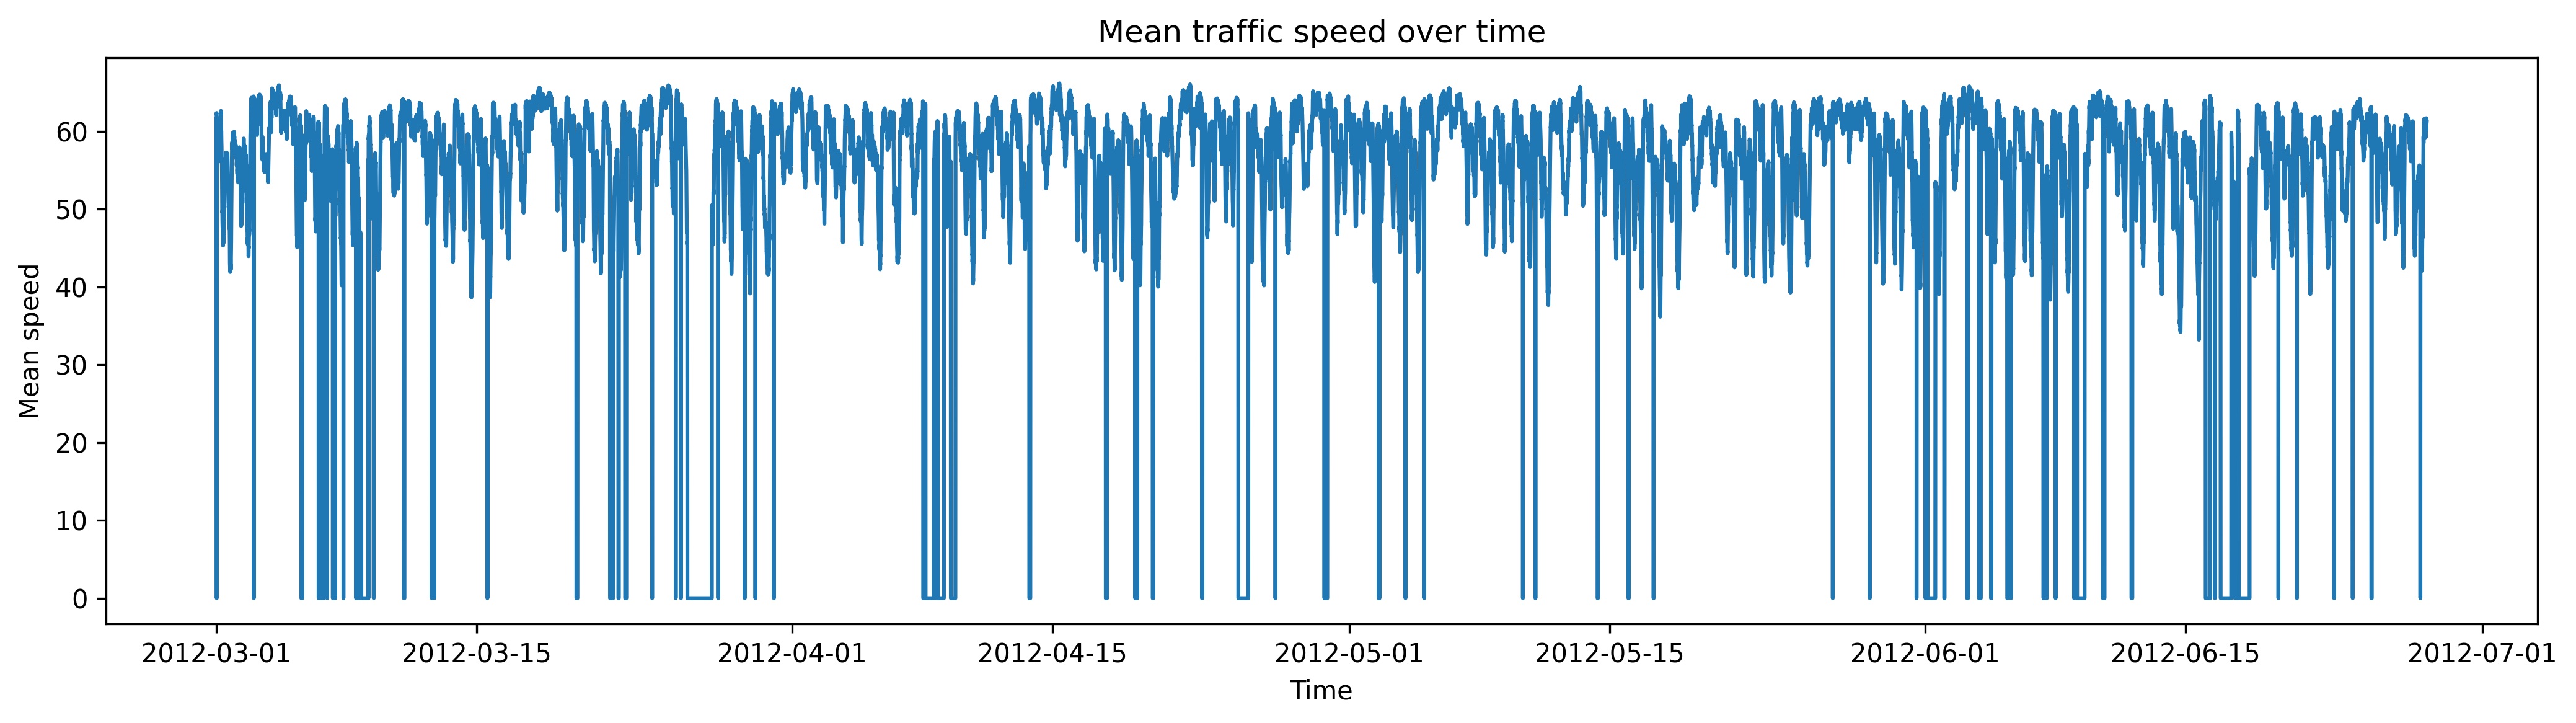
\includegraphics[width=\textwidth]{img/data_analysis/mean_speed_with_zeros}

    \vspace{0.3cm}

    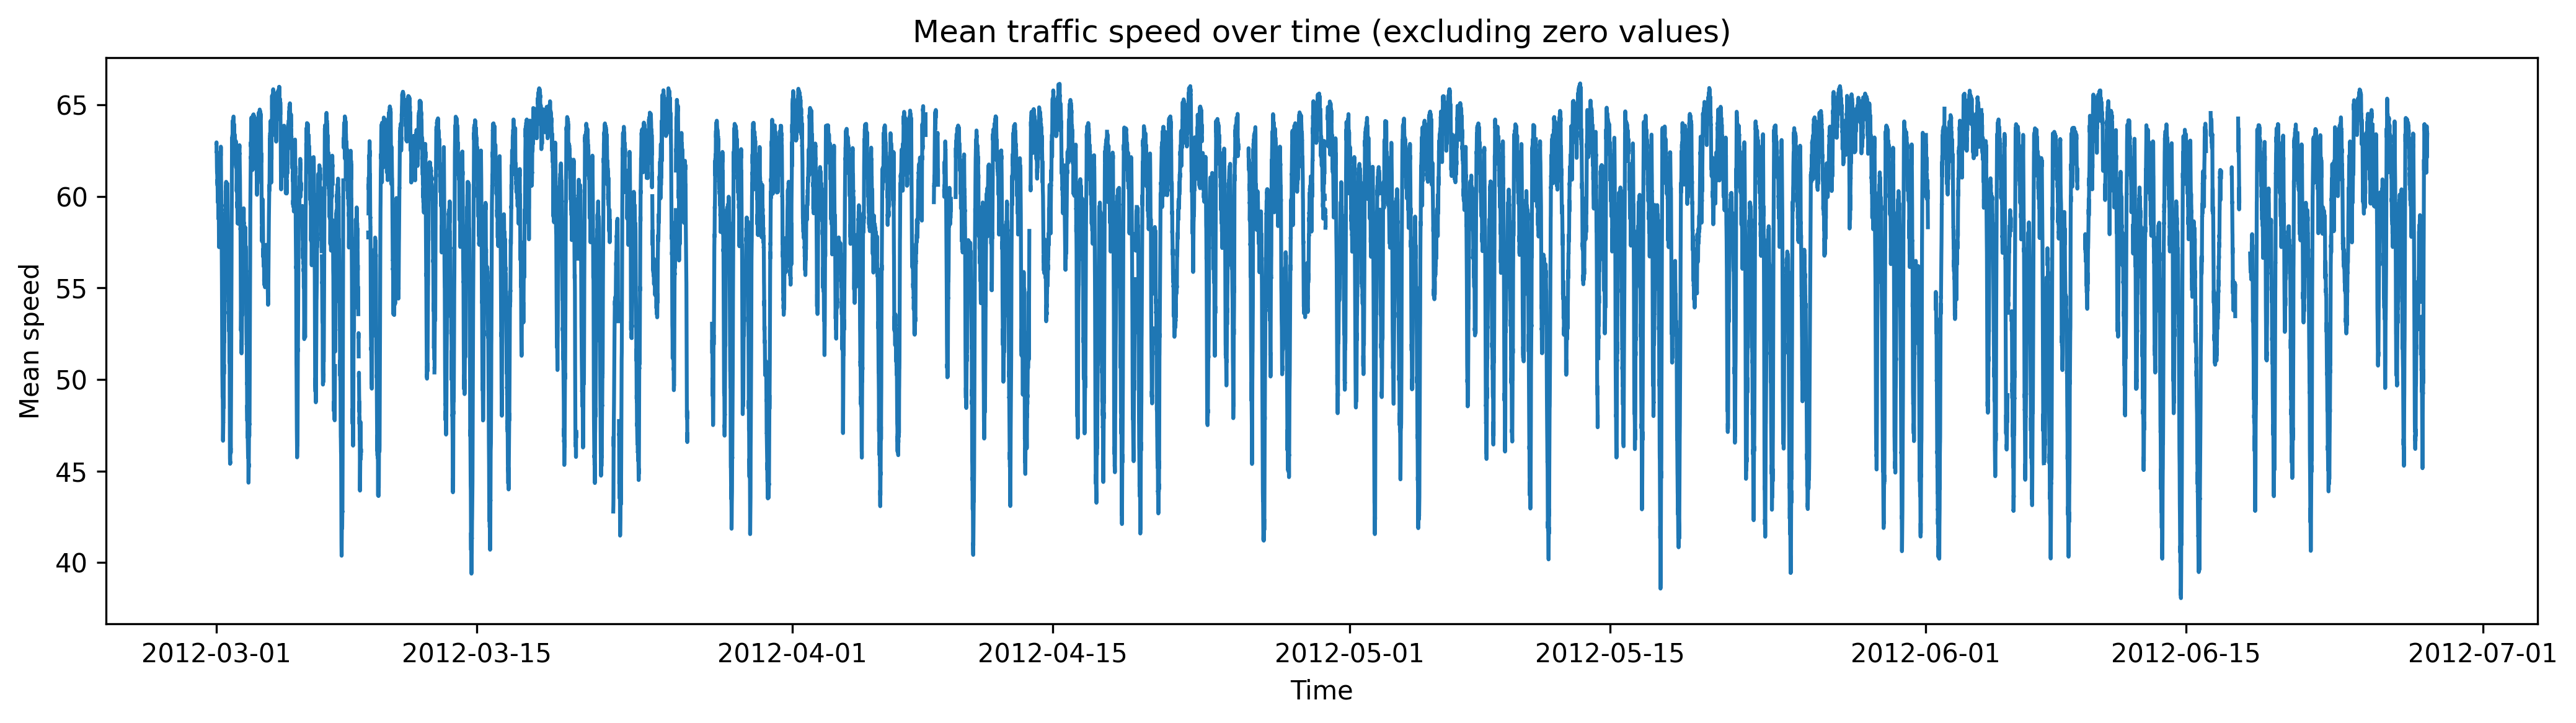
\includegraphics[width=\textwidth]{img/data_analysis/mean_speed_without_zeros}

    \caption{Mean traffic speed over time before (top) and after (bottom) excluding zero values.
    Removing zero-valued measurements eliminates the abrupt drops to zero while preserving the temporal traffic patterns.}
    \label{fig:mean_speed_zero_comparison}
\end{figure}


The valid traffic measurements also exhibit strong temporal structure.
Aggregating traffic speeds by hour of the day reveals a clear daily
seasonality, with average speeds decreasing during typical congestion periods
and increasing again during less congested hours. However, aggregating all
days together partially hides differences between working days and weekends.

Figure~\ref{fig:temporal_patterns} therefore compares the hourly traffic-speed
profiles obtained separately for weekdays and weekends.
Weekdays exhibit two pronounced reductions in average speed, occurring around
8:00 and 17:00 and corresponding to the typical morning and afternoon commuting periods.
In contrast, weekends show a smoother daily profile, with generally higher speeds during these hours.
The figure therefore reveals a weekly component in addition to the daily seasonality.

These observations confirm that the traffic series contains meaningful
temporal dependencies at multiple time scales and motivate the use of a
temporal forecasting model in the subsequent experiments.

\begin{figure}[t]
    \centering
    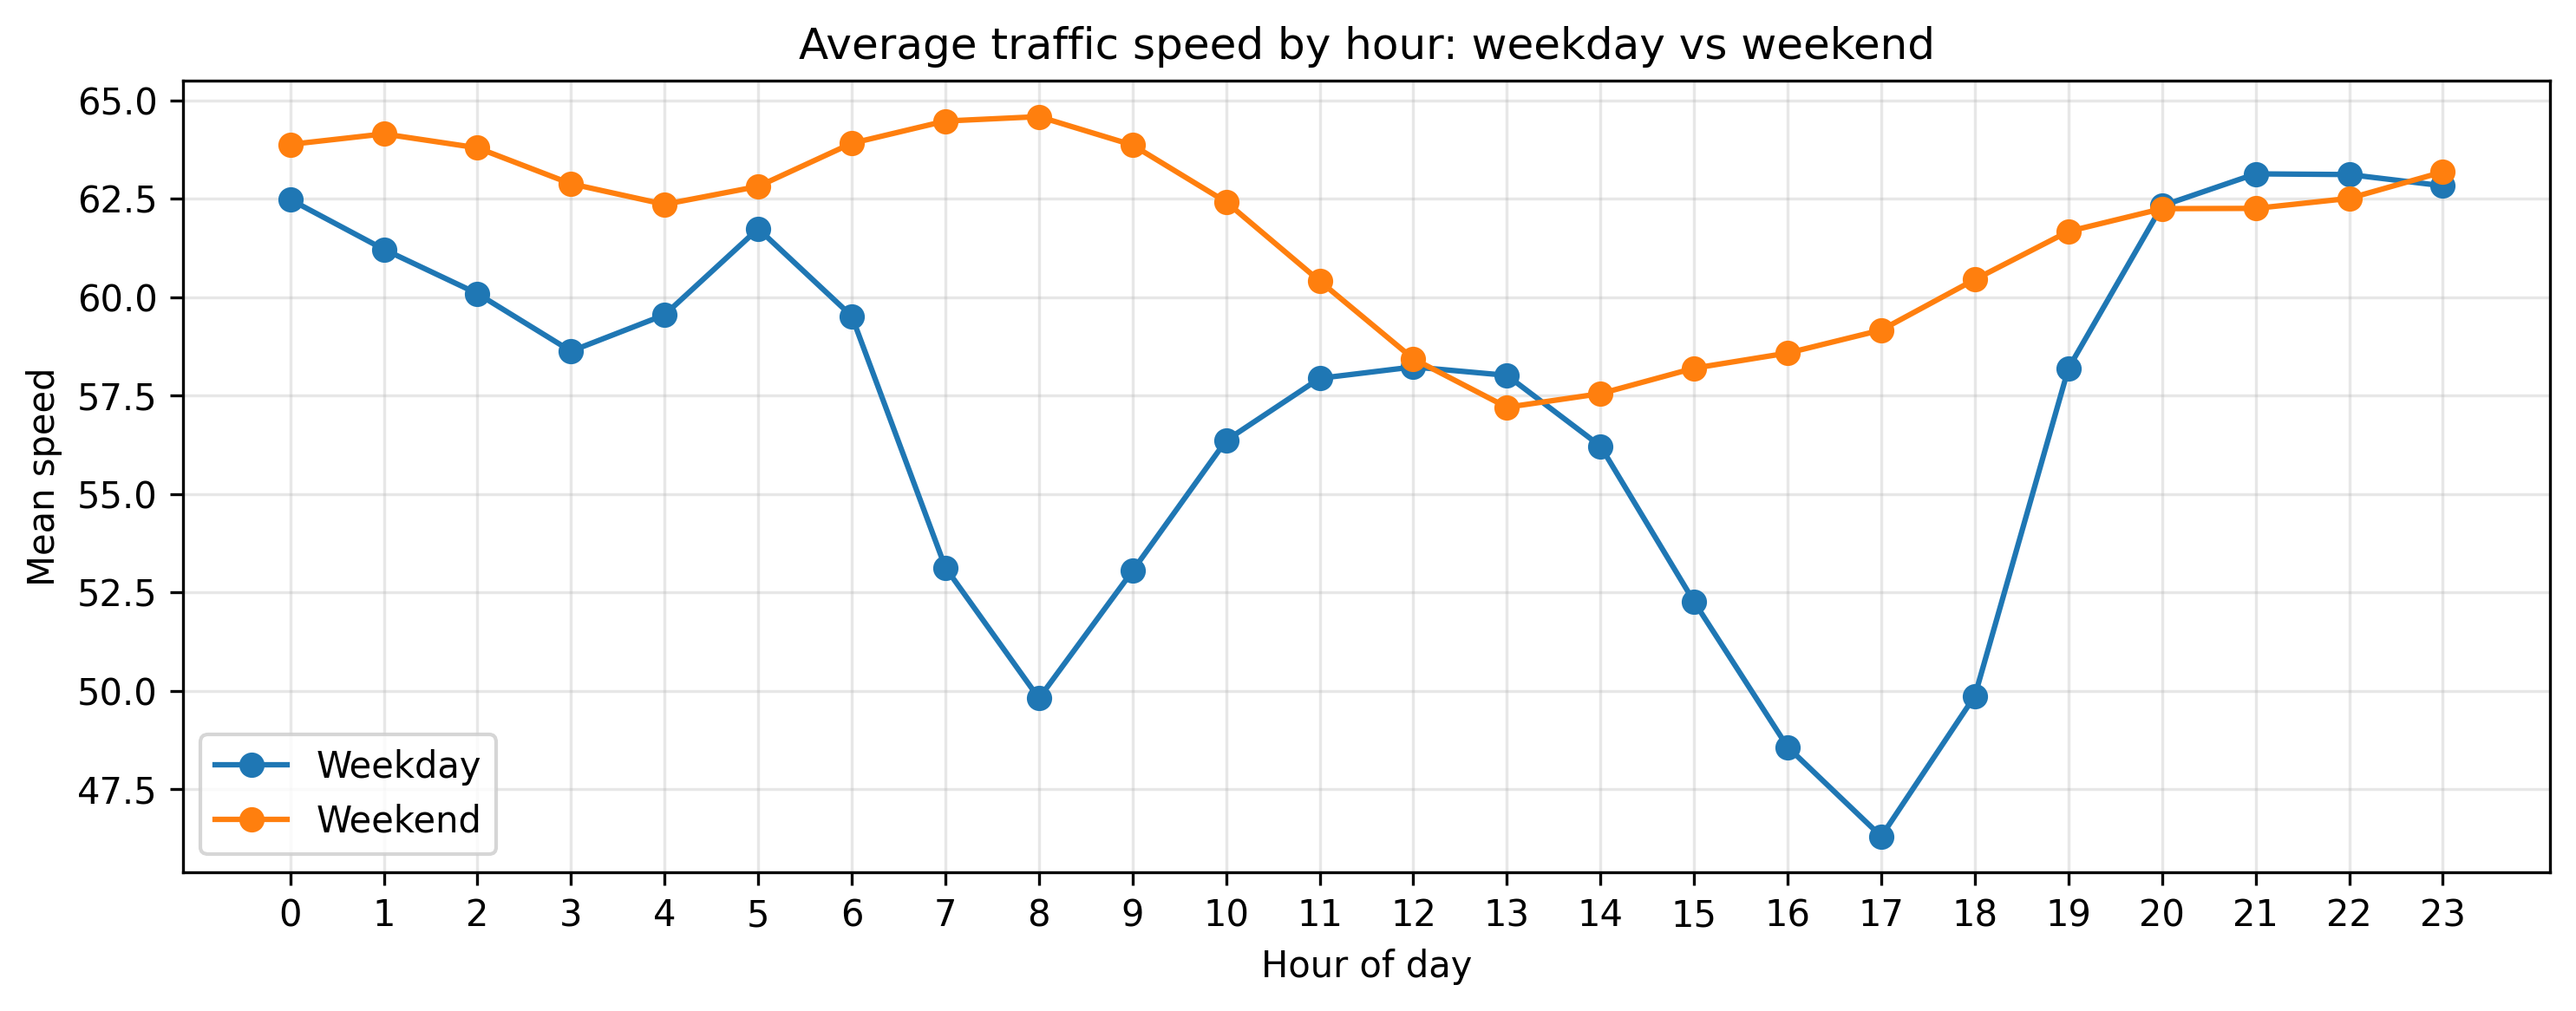
\includegraphics[width=0.75\linewidth]
    {img/data_analysis/weekday_vs_weekend}
    \caption{Average traffic-speed profile by hour of the day, computed
    separately for weekdays and weekends. The different profiles highlight
    both daily and weekly temporal patterns in the METR-LA measurements.}
    \label{fig:temporal_patterns}
\end{figure}

Finally, the distribution of traffic speeds was examined at the individual
sensor level. Considerable heterogeneity was observed across the network, since
the mean traffic speed ranges from approximately 30.89 to 67.73 across
sensors, while the corresponding temporal standard deviations range from
approximately 1.99 to 23.94. Therefore, different sensors exhibit distinct
traffic levels and degrees of variability.

This heterogeneity is particularly relevant for preprocessing, since applying
a single global normalization would ignore the different operating ranges of
individual sensors. For this reason, the normalization strategy described in
Section~\ref{subsec:windowing} estimates separate statistics for each sensor.

Overall, the exploratory analysis identifies two main properties that guide
the preprocessing and modeling choices adopted in this work: a non-negligible
amount of unavailable measurements encoded as zeros, and strong but
heterogeneous temporal traffic patterns across the sensor network.


\subsection{Leakage-Free Data Partitioning}
\label{subsec:splitting}

To preserve the temporal nature of the forecasting problem and prevent
information leakage, the original time series was partitioned
chronologically, without shuffling, into training, validation, and test sets
using a 70\%-10\%-20\% split. Importantly, the partition was performed on
the raw time series before normalization and temporal window construction.

The resulting partitions are summarized in
Table~\ref{tab:chronological_split}. The training set contains 23990
timestamps, followed by 3427 validation timestamps and 6855 test
timestamps. This ordering ensures that validation and test observations
always occur later in time than the observations used for model training.

\begin{table}[t]
    \centering
    \caption{Chronological partition of the original METR-LA time series
    before preprocessing and temporal window construction.}
    \label{tab:chronological_split}
    \begin{tabular}{lrrl}
        \toprule
        Split & Proportion & Timestamps & Time period \\
        \midrule
        Training   & 70\% & 23990 &
        Mar.\ 1 00:00 -- May 23 07:05 \\
        Validation & 10\% & 3427 &
        May 23 07:10 -- Jun.\ 4 04:40 \\
        Test       & 20\% & 6855 &
        Jun.\ 4 04:45 -- Jun.\ 27 23:55 \\
        \bottomrule
    \end{tabular}
\end{table}

All data-dependent preprocessing operations were subsequently fitted using
the training partition only. In particular, the per-sensor normalization
statistics were estimated exclusively from training observations and then
reused unchanged for validation and test data.

Temporal windows were also constructed independently within each partition.
Consequently, an input--target pair can never cross a split boundary. For
example, a training input window cannot use observations from the validation
period as future targets. This procedure preserves the chronological
separation between model development and final evaluation.

\subsection{Normalization and Temporal Windowing}
\label{subsec:windowing}

As discussed in Section~\ref{subsec:eda}, traffic-speed distributions vary
substantially across sensors. For this reason, the data were standardized
independently for each sensor rather than using global statistics shared
across the complete network.

For each sensor $n$, the mean $\mu_n$ and standard deviation $\sigma_n$ were
estimated exclusively from the valid observations in the training partition.
Each available traffic-speed observation $x_{t,n}$ was then transformed as

\begin{equation}
    \tilde{x}_{t,n}
    =
    \frac{x_{t,n}-\mu_n}{\sigma_n}.
    \label{eq:normalization}
\end{equation}

The same training statistics were subsequently applied without modification
to the validation and test partitions. This prevents information from future
partitions from influencing the preprocessing procedure.

After preprocessing and normalization, each chronological partition was
independently transformed into input--target pairs using a sliding-window
procedure. Given an input-history length $H=12$ and a forecasting window
$F=12$, a sample generated at time $t$ consists of the previous 12 traffic
observations and the following 12 observations to be predicted.

More formally, the input and target windows are defined as

\begin{equation}
    \mathbf{X}_t
    =
    \left[
        \tilde{\mathbf{x}}_{t-H+1},
        \ldots,
        \tilde{\mathbf{x}}_{t}
    \right]
    \in \mathbb{R}^{H \times N},
    \label{eq:input_window}
\end{equation}

and

\begin{equation}
    \mathbf{Y}_t
    =
    \left[
        \tilde{\mathbf{x}}_{t+1},
        \ldots,
        \tilde{\mathbf{x}}_{t+F}
    \right]
    \in \mathbb{R}^{F \times N},
    \label{eq:target_window}
\end{equation}

where $N=207$ is the number of sensors. Since measurements are sampled every
five minutes, both $H=12$ and $F=12$ correspond to one hour of traffic
observations.


Although the models jointly predict all $F=12$ future steps, the main
evaluation is performed at three representative forecasting horizons:
$t+3$, $t+6$, and $t+12$, corresponding respectively to 15, 30, and
60 minutes into the future. This allows performance to be analyzed as the
forecasting task becomes progressively more difficult with increasing
prediction horizon.


The windowing procedure was applied jointly to the traffic values and their
availability masks. Consequently, each input window is associated with an
input mask indicating which historical observations are available, while
each target window is associated with a target mask identifying the entries
that can contribute to the training loss and evaluation metrics.

Partially observed windows are therefore retained whenever useful information
is available, rather than being discarded entirely because of a small number
of missing sensor measurements. As described in
Section~\ref{subsec:missing}, unavailable target entries never contribute to
model optimization or performance evaluation.


The resulting preprocessing pipeline therefore preserves the chronological
structure of the forecasting problem, estimates all data-dependent
transformations exclusively from the training period, and explicitly tracks
unavailable observations through masks. The same processed input-target
windows are used by all forecasting approaches described in the following
section, ensuring that differences in performance are attributable to the
forecasting models rather than to different data-processing procedures.


\subsection{Missing-Value Handling}
\label{subsec:missing}

Based on the exploratory analysis in
Section~\ref{subsec:eda}, zero-valued traffic measurements were interpreted
as unavailable observations and replaced with missing values before further
processing.
After normalization and temporal window construction, missing values were
handled differently in the input histories X and forecasting targets Y,
since imputing a target would create
artificial ground-truth values and could bias both training and evaluation.

\paragraph{Input histories.}

Missing observations in each input window were handled through a limited interpolation procedure.
For each sensor independently, only short
internal gaps of at most three consecutive timestamps were interpolated, and
only when valid observations were available on both sides of the gap. Longer
gaps and missing values at the boundaries of an input window were left
unchanged.

This conservative strategy reduces isolated sensor dropouts while avoiding
the reconstruction of long unavailable periods from potentially unrelated
observations. Before interpolation, missing values accounted for
approximately 7.13\%, 7.00\%, and 12.13\% of the input values in the
training, validation, and test windows, respectively. After short-gap
interpolation, these proportions decreased to approximately 6.85\%, 6.83\%,
and 11.92\%.

Therefore, interpolation only
moderately reduces the overall amount of missing data. This is expected
because the procedure deliberately targets short internal gaps while
preserving longer periods of sensor unavailability.

Input windows for which all sensors were unavailable throughout the complete
history were removed, since they contain no temporal information from which a
forecast can be produced. In contrast, a window was retained when only a
subset of sensors was fully unavailable, because observations from the
remaining sensors may still provide useful information, particularly for the
graph-temporal model.

After this filtering step, residual missing input values were replaced by
zero in the standardized domain. Since normalization is performed separately
for each sensor using training statistics, this value corresponds to the
training mean of that sensor rather than to a physical traffic speed of zero.
An input availability mask was retained to distinguish observed from missing
measurements.

\paragraph{Forecasting targets.}

A stricter policy was adopted for the forecasting targets. Target values were
never interpolated or semantically imputed, since doing so would introduce
synthetic ground truth into the optimization and evaluation procedures.
Instead, a binary target-availability mask was constructed and propagated
throughout the complete pipeline.

Windows with no valid target observations over the complete forecasting
period were removed. Partially observed target windows were retained, while
missing target entries were numerically replaced with finite placeholder
values only to maintain valid tensor representations. These entries were
always excluded from the loss and evaluation metrics through the target
mask and therefore never contributed to model optimization or reported
performance.

After filtering fully unavailable input and target windows, the final dataset
contains 22817 training samples, 3240 validation samples, and 6224 test
samples, as reported in Table~\ref{tab:final_dataset}.

\begin{table}[t]
    \centering
    \caption{Number of temporal samples retained after missing-data
    processing and filtering.}
    \label{tab:final_dataset}
    \begin{tabular}{lr}
        \toprule
        Split & Final samples \\
        \midrule
        Training   & 22817 \\
        Validation & 3240 \\
        Test       & 6224 \\
        \bottomrule
    \end{tabular}
\end{table}
Despite the missing periods identified in the raw data,
target availability remains high at all evaluated horizons,
ranging from approximately 95\% to 97\% depending on the split and forecast
horizon, providing a sufficiently large set of valid
observations for model training and evaluation.


\section{Forecasting Methodology}
\label{sec:methodology}

\subsection{Probabilistic Forecasting Formulation}
\label{subsec:probabilistic}

The forecasting task is formulated probabilistically through conditional
quantile estimation. Rather than predicting a single future traffic speed,
the neural forecasting models estimate three quantiles for each sensor and
forecasting step,

\begin{equation}
    \mathcal{Q} = \{0.1, 0.5, 0.9\}.
    \label{eq:quantiles}
\end{equation}

For an input window $\mathbf{X}_t$, the models therefore produce

\begin{equation}
    \hat{\mathbf{Y}}_t
    \in
    \mathbb{R}^{F \times N \times |\mathcal{Q}|},
    \label{eq:probabilistic_output}
\end{equation}

where $F=12$ is the forecasting window, $N=207$ is the number of sensors,
and $|\mathcal{Q}|=3$ is the number of predicted quantiles.

The median prediction $\hat{y}^{(0.5)}$ is used as the point forecast when
computing deterministic metrics such as MAE and RMSE. The lower and upper
quantiles define the predictive interval

\begin{equation}
    \left[
        \hat{y}^{(0.1)},
        \hat{y}^{(0.9)}
    \right],
    \label{eq:prediction_interval}
\end{equation}

which has a nominal coverage probability of $80\%$. This formulation makes it
possible to evaluate point forecasting accuracy and predictive uncertainty
using a single model.


The models are trained using the Pinball Loss. For a target value $y$, a
predicted quantile $\hat{y}^{(q)}$, and a quantile level $q$, the loss is
defined as

\begin{equation}
    \mathcal{L}_{q}
    \left(y,\hat{y}^{(q)}\right)
    =
    \max
    \left(
        q\left(y-\hat{y}^{(q)}\right),
        (q-1)\left(y-\hat{y}^{(q)}\right)
    \right).
    \label{eq:pinball_loss}
\end{equation}

Unlike a symmetric regression loss, the Pinball Loss penalizes
underestimation and overestimation differently according to the target
quantile. Minimizing it therefore allows the model to estimate different
regions of the conditional target distribution rather than only its central
value.


Since some target observations are unavailable, the Pinball Loss is computed
only over valid target entries. During training, consider a mini-batch of
$B$ samples. Let $b \in \{1,\ldots,B\}$ denote the sample index,
$h \in \{1,\ldots,F\}$ the forecast step, and
$n \in \{1,\ldots,N\}$ the sensor index. The binary mask
$m_{b,h,n} \in \{0,1\}$ indicates whether the corresponding target value is
available.

For each mini-batch, the training loss is obtained by averaging the Pinball
Loss over all valid target entries and over all predicted quantiles:

\begin{equation}
    \mathcal{L}_{\mathrm{masked}}
    =
    \frac{
        \displaystyle
        \sum_{b=1}^{B}
        \sum_{h=1}^{F}
        \sum_{n=1}^{N}
        m_{b,h,n}
        \sum_{q\in\mathcal{Q}}
        \mathcal{L}_{q}
        \left(
            y_{b,h,n},
            \hat{y}_{b,h,n}^{(q)}
        \right)
    }{
        \displaystyle
        |\mathcal{Q}|
        \sum_{b=1}^{B}
        \sum_{h=1}^{F}
        \sum_{n=1}^{N}
        m_{b,h,n}
    }.
    \label{eq:masked_pinball}
\end{equation}

Consequently, unavailable target values do not contribute to the loss,
while every valid target contributes once for each quantile in
$\mathcal{Q}$. This is consistent with the missing-data strategy described
in Section~\ref{subsec:missing}.


\subsection{Persistence Baseline}
\label{subsec:persistence}

A persistence model is used as the simplest forecasting baseline. For each
sensor, the value at the final time step of the input window is repeated
across the complete forecasting horizon. The prediction for sensor $n$ at
any future step $h$ is therefore

\begin{equation}
    \hat{y}_{t+h,n} = x_{t,n},
    \qquad h=1,\ldots,F.
    \label{eq:persistence}
\end{equation}

The persistence baseline contains no trainable parameters and does not
explicitly model either temporal dynamics or spatial interactions. It
therefore provides a simple reference for determining whether the learned
models extract useful predictive information from the historical traffic
sequence.


\subsection{Temporal GRU}
\label{subsec:gru}

The first learned forecasting model is a temporal Gated Recurrent Unit
(GRU), which serves as the no-graph baseline.
Each sensor is
processed independently using its own sequence of historical traffic
observations, while the GRU parameters are shared across all sensors.

For a given sensor $n$, the input sequence

\begin{equation}
    \left[
        \tilde{x}_{t-H+1,n},
        \ldots,
        \tilde{x}_{t,n}
    \right]
\end{equation}

is processed by the same recurrent network. No information from other
sensors is exchanged during the forward pass. The model therefore provides a
controlled no-graph baseline against which the contribution of spatial
message passing can be evaluated.

The selected temporal architecture consists of a two-layer GRU with hidden
dimension 64. The final hidden representation of each sensor is passed to a
linear output layer that jointly predicts all $F=12$ future steps and all
three quantiles. For each sensor, the output layer therefore produces

\begin{equation}
    F \times |\mathcal{Q}| = 12 \times 3 = 36
\end{equation}

values, which are reshaped into the corresponding forecast-step and quantile
dimensions.

The complete model contains 40164 trainable parameters. Because the same
network is applied to every sensor, the parameter count does not scale with
the number of nodes in the traffic network.


\subsection{Graph Representation and Diffusion-Style Message Passing}
\label{subsec:graph}

Spatial dependencies are introduced through the sensor graph provided with
METR-LA \citep{li2018dcrnn}. Each traffic sensor corresponds to a graph node, while the adjacency
matrix

\begin{equation}
    \mathbf{A} \in \mathbb{R}^{N \times N}
\end{equation}

encodes directed, weighted connections between sensors. Throughout this work,
the convention is that $A_{ij}$ represents the weight assigned at node $i$
to the message received from node $j$. Therefore, row $i$ contains the
weights used to aggregate information into node $i$.

The provided adjacency matrix already contains self-connections. Therefore,
no additional identity matrix is added to $\mathbf{A}$ before normalization.
This avoids introducing artificial self-loops or modifying the relative
weights of the graph supplied with the dataset.

Before message passing, the adjacency matrix is row-normalized as

\begin{equation}
    \mathbf{P} = \mathbf{D}^{-1}\mathbf{A},
    \label{eq:row_normalization}
\end{equation}

where $\mathbf{D}$ is the diagonal matrix of row sums,

\begin{equation}
    D_{ii} = \sum_j A_{ij}.
\end{equation}

Under the adopted convention, the one-step propagated representation of node
$i$ is therefore

\begin{equation}
    (\mathbf{P}\mathbf{X})_i
    =
    \sum_j P_{ij}\mathbf{X}_j,
    \label{eq:graph_aggregation}
\end{equation}

so that node $i$ receives a weighted combination of the representations of
the nodes $j$ connected to it.

Spatial information is incorporated through a diffusion-style message-passing
layer, conceptually inspired by diffusion-based graph modeling for traffic
forecasting \citep{li2018dcrnn}.
This formulation implements a compact unidirectional multi-hop propagation
operator rather than the bidirectional diffusion convolution of DCRNN.
Only powers of the row-normalized propagation matrix PP are considered,
with a separate learnable transformation $W_k$ for each propagation depth.
Given node features $\mathbf{X}$, the layer computes

\begin{equation}
    \mathbf{H}
    =
    \sum_{k=0}^{K}
    \mathbf{P}^{k}\mathbf{X}\mathbf{W}_{k}
    +
    \mathbf{b},
    \label{eq:diffusion}
\end{equation}

where $K$ controls the maximum diffusion depth and each $\mathbf{W}_{k}$ is
a learnable projection associated with a different propagation step. The
$k=0$ term, for which $\mathbf{P}^{0}=\mathbf{I}$, directly preserves the
node's own representation, while the terms with $k\geq1$ incorporate
information propagated through the graph.

For the main configuration, $K=2$, yielding

\begin{equation}
    \mathbf{H}
    =
    \mathbf{X}\mathbf{W}_{0}
    +
    \mathbf{P}\mathbf{X}\mathbf{W}_{1}
    +
    \mathbf{P}^{2}\mathbf{X}\mathbf{W}_{2}
    +
    \mathbf{b}.
    \label{eq:diffusion_k2}
\end{equation}

The first term provides an explicit transformation of each node's own
representation, while the remaining terms incorporate information propagated
over one and two graph transitions. Since the diagonal entries already
present in $\mathbf{A}$ are preserved by the row normalization, the
one-step and two-step diffusion terms may themselves also contain
self-information.


\subsection{Graph-Temporal Architecture}
\label{subsec:graph_temporal}

The main forecasting model combines the diffusion-style message-passing operation
described in
Section~\ref{subsec:graph} with recurrent temporal modeling. The architecture
is composed of two consecutive graph-temporal blocks. Each block first
propagates information between sensors through diffusion-style message passing and
then applies a GRU to model the temporal evolution of the resulting node
representations (Figure \ref{fig:graphtemporalarchitecture}).

Given an input window, diffusion is applied independently at each temporal
step, allowing every sensor representation to incorporate information from
its graph neighborhood. The resulting sequence of spatial representations is
then processed by a GRU independently for each node, with recurrent
parameters shared across sensors. The first block preserves the complete
temporal sequence so that it can be processed by the second diffusion--GRU
block.

The final temporal representation is passed to a linear probabilistic head
that directly predicts the 12 future steps for the three quantile levels
defined in Section~\ref{subsec:probabilistic}. As in the Temporal GRU, the
complete forecasting window is generated in a single forward pass rather
than recursively feeding previous predictions back into the model.

The selected graph-temporal model uses a graph hidden dimension of 64, a GRU
hidden dimension of 64, one GRU layer per graph-temporal block, two
graph-temporal blocks, and a diffusion depth of $K=2$. The complete
architecture contains 64868 trainable parameters.

\begin{figure}[t]
    \centering
    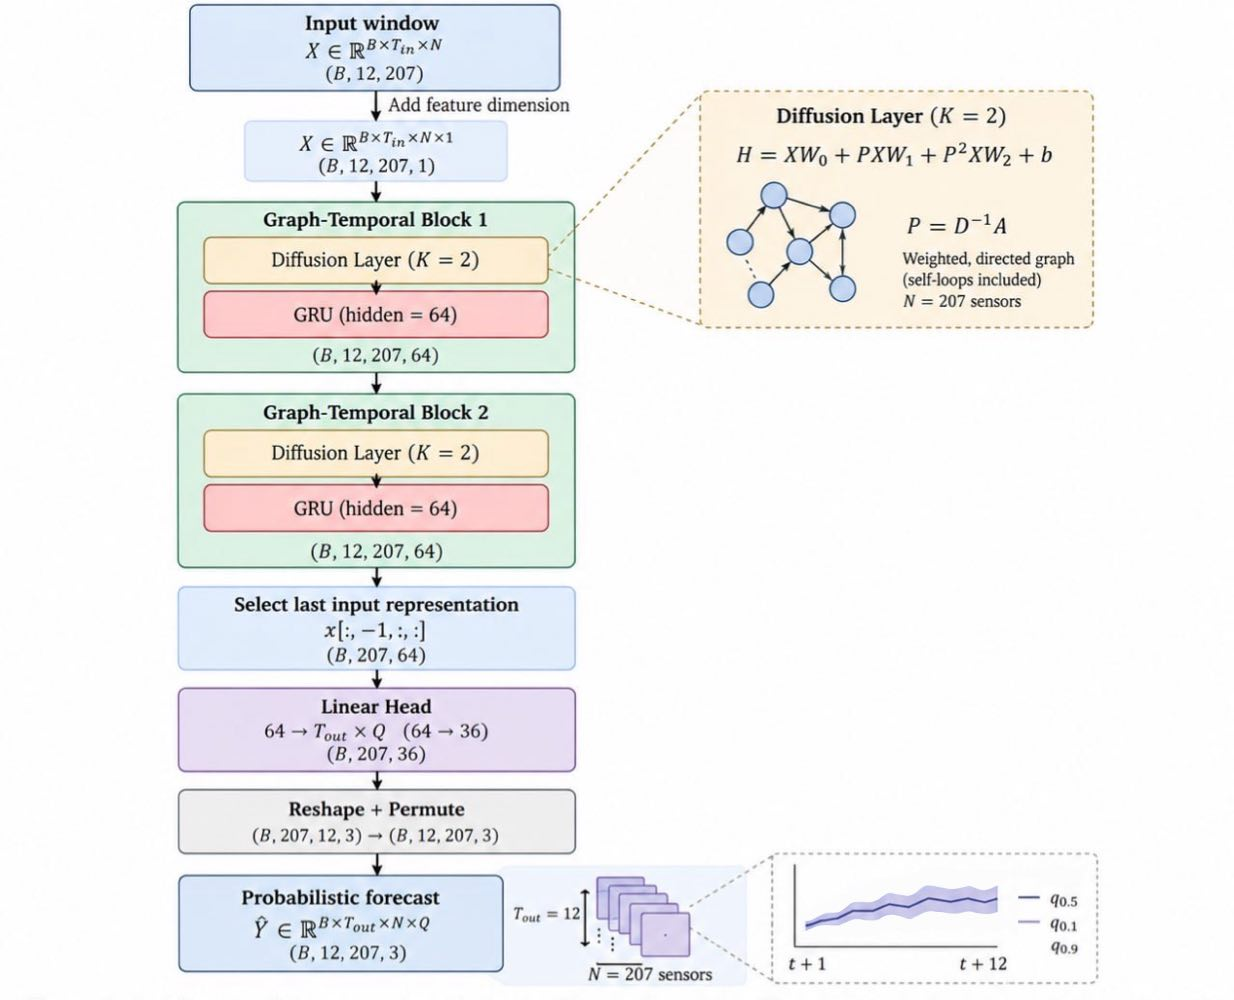
\includegraphics[width=\linewidth]{img/graphtemporalarchitecture}
    \caption{Architecture of the proposed graph-temporal forecasting model.}
    \label{fig:graphtemporalarchitecture}
\end{figure}

\section{Experimental Setup}
\label{sec:experimental_setup}

\subsection{Training Protocol}
\label{subsec:training}

Both the Temporal GRU and the Graph-Temporal model were trained using the
masked Pinball Loss defined in Equation~\ref{eq:masked_pinball}. Model
parameters were optimized with Adam using mini-batches of 64 samples.

Training was performed for a maximum of 200 epochs with early stopping based
on the validation Pinball Loss and a patience of 10 epochs. Whenever the
validation loss improved, the corresponding model checkpoint was retained.
Training was terminated if no further improvement was observed for 10
consecutive epochs, and the checkpoint associated with the lowest validation
loss was used for subsequent evaluation.

Both neural models use direct multi-horizon forecasting: all 12 future time
steps and the three target quantiles are predicted simultaneously from the
input history.

No test-set information was used for hyperparameter selection, early stopping,
or model calibration. The test partition was accessed only after the model
configuration had been selected using the training and validation partitions.


\subsection{Hyperparameter Selection}
\label{subsec:hyperparameters}

Hyperparameters were selected exclusively according to the validation
Pinball Loss. Separate grid searches were performed for the Temporal GRU and
the Graph-Temporal model, since the two architectures expose different
model-specific parameters. The search spaces and selected configurations are
summarized in Table~\ref{tab:hyperparameters}.

\begin{table}[t]
    \centering
    \caption{Hyperparameter search spaces and selected configurations for the
    two neural forecasting models.}
    \label{tab:hyperparameters}
    \begin{tabular}{lll}
        \toprule
        Model & Hyperparameter & Values \\
        \midrule

        Temporal GRU
        & Hidden dimension & $\{32,\mathbf{64}\}$ \\
        & GRU layers & $\{1,\mathbf{2}\}$ \\
        & Learning rate & $\{\mathbf{5\times10^{-4}},10^{-3}\}$ \\
        \midrule

        Graph-Temporal
        & Graph hidden dimension & $\{32,\mathbf{64}\}$ \\
        & GRU hidden dimension & $\mathbf{64}$ \\
        & GRU layers per block & $\{\mathbf{1},2\}$ \\
        & Learning rate & $\{\mathbf{5\times10^{-4}},10^{-3}\}$ \\
        & Diffusion depth $K$ & $\mathbf{2}$ \\
        & Graph-temporal blocks & $\mathbf{2}$ \\
        \bottomrule
    \end{tabular}
\end{table}

Selected values are highlighted in bold. The diffusion depth and number of
graph-temporal blocks were kept fixed during the main hyperparameter search;
the effect of changing the diffusion depth is investigated separately in
Section~\ref{subsec:diffusion_depth}.

For the Temporal model, the selected configuration uses a hidden dimension of
64, two recurrent layers, and a learning rate of $5\times10^{-4}$. The best
checkpoint was obtained at epoch 78, with a validation Pinball Loss of
0.1240.

For the Graph-Temporal model, the selected configuration uses a graph hidden
dimension of 64, a GRU hidden dimension of 64, one recurrent layer per
graph-temporal block, and a learning rate of $5\times10^{-4}$. With two
blocks and diffusion depth $K=2$, the best checkpoint was obtained at epoch
106, reaching a validation Pinball Loss of 0.1133.


The learning curves of the selected configurations are shown in
Figure~\ref{fig:learning_curves}. For both models, the training loss decreases
progressively, while the validation loss eventually reaches a minimum and
ceases to improve. The selected checkpoints therefore correspond to the
minimum validation loss rather than to the final training epoch, consistently
with the early-stopping procedure described in
Section~\ref{subsec:training}.

\begin{figure}[t]
    \centering

    \begin{subfigure}[b]{0.48\linewidth}
        \centering
        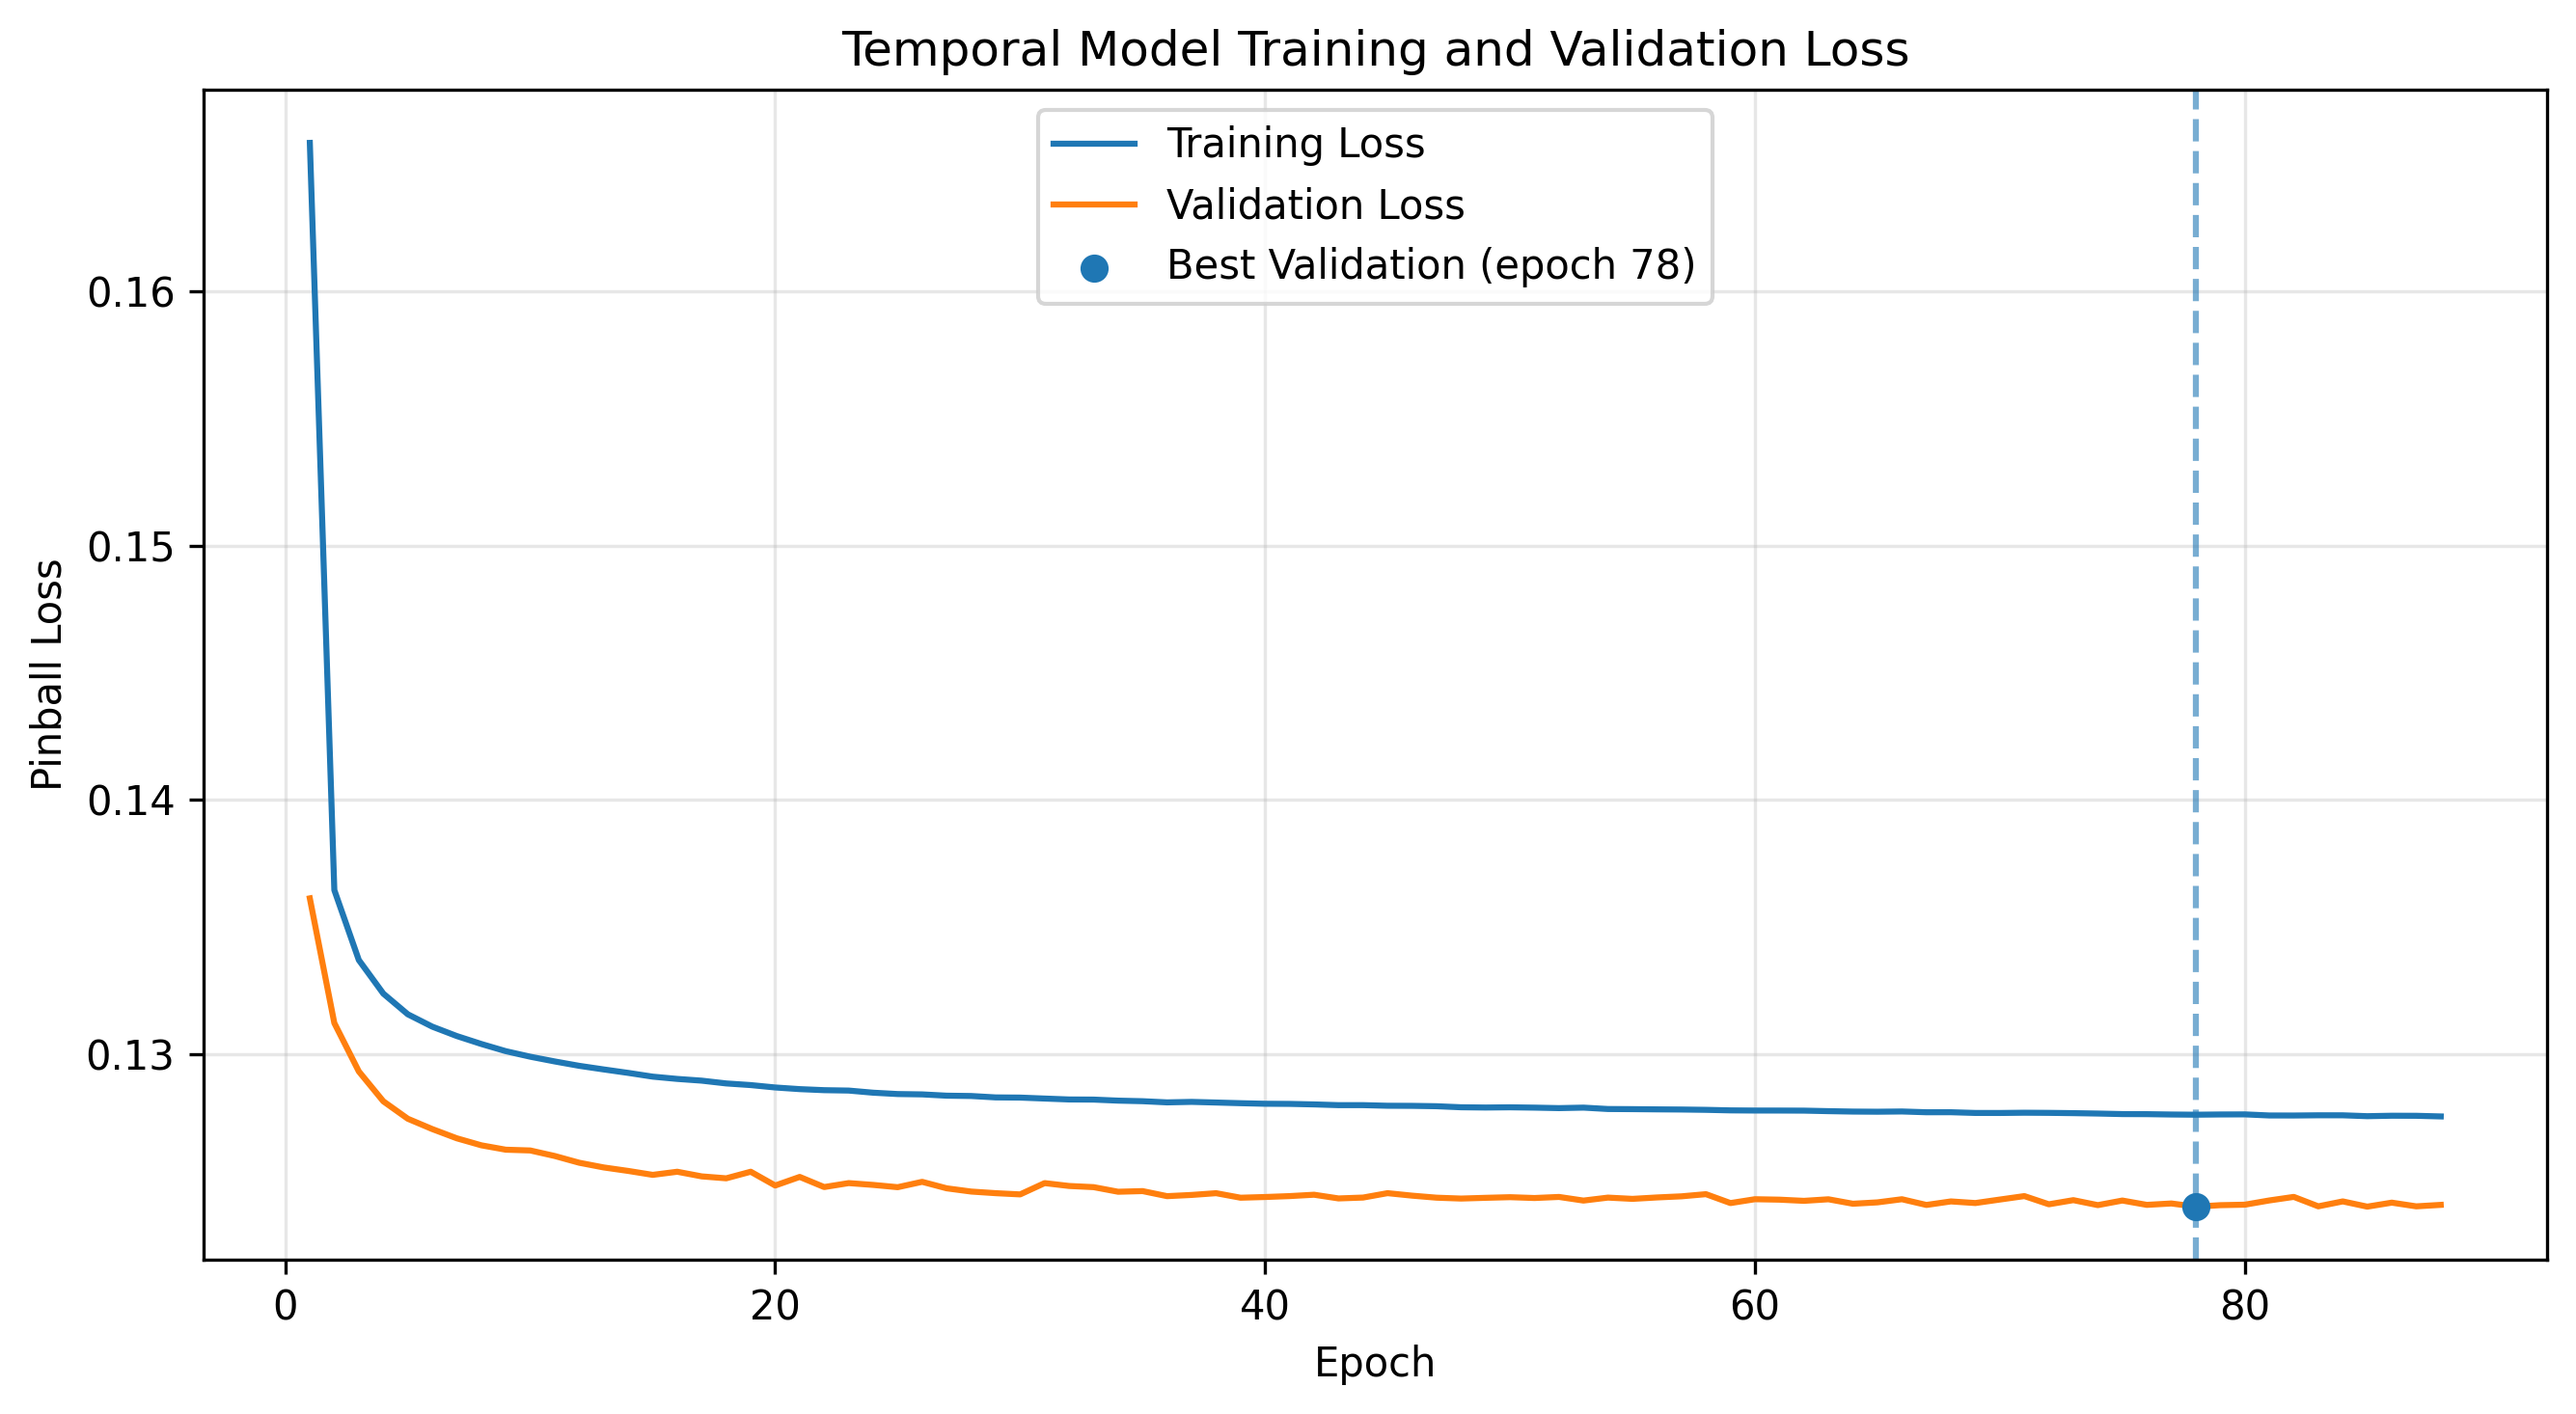
\includegraphics[width=\linewidth]{img/temporal_gru/learning_curves}
        \caption{Temporal model.}
        \label{fig:gru_learning_curve}
    \end{subfigure}
    \hfill
    \begin{subfigure}[b]{0.48\linewidth}
        \centering
        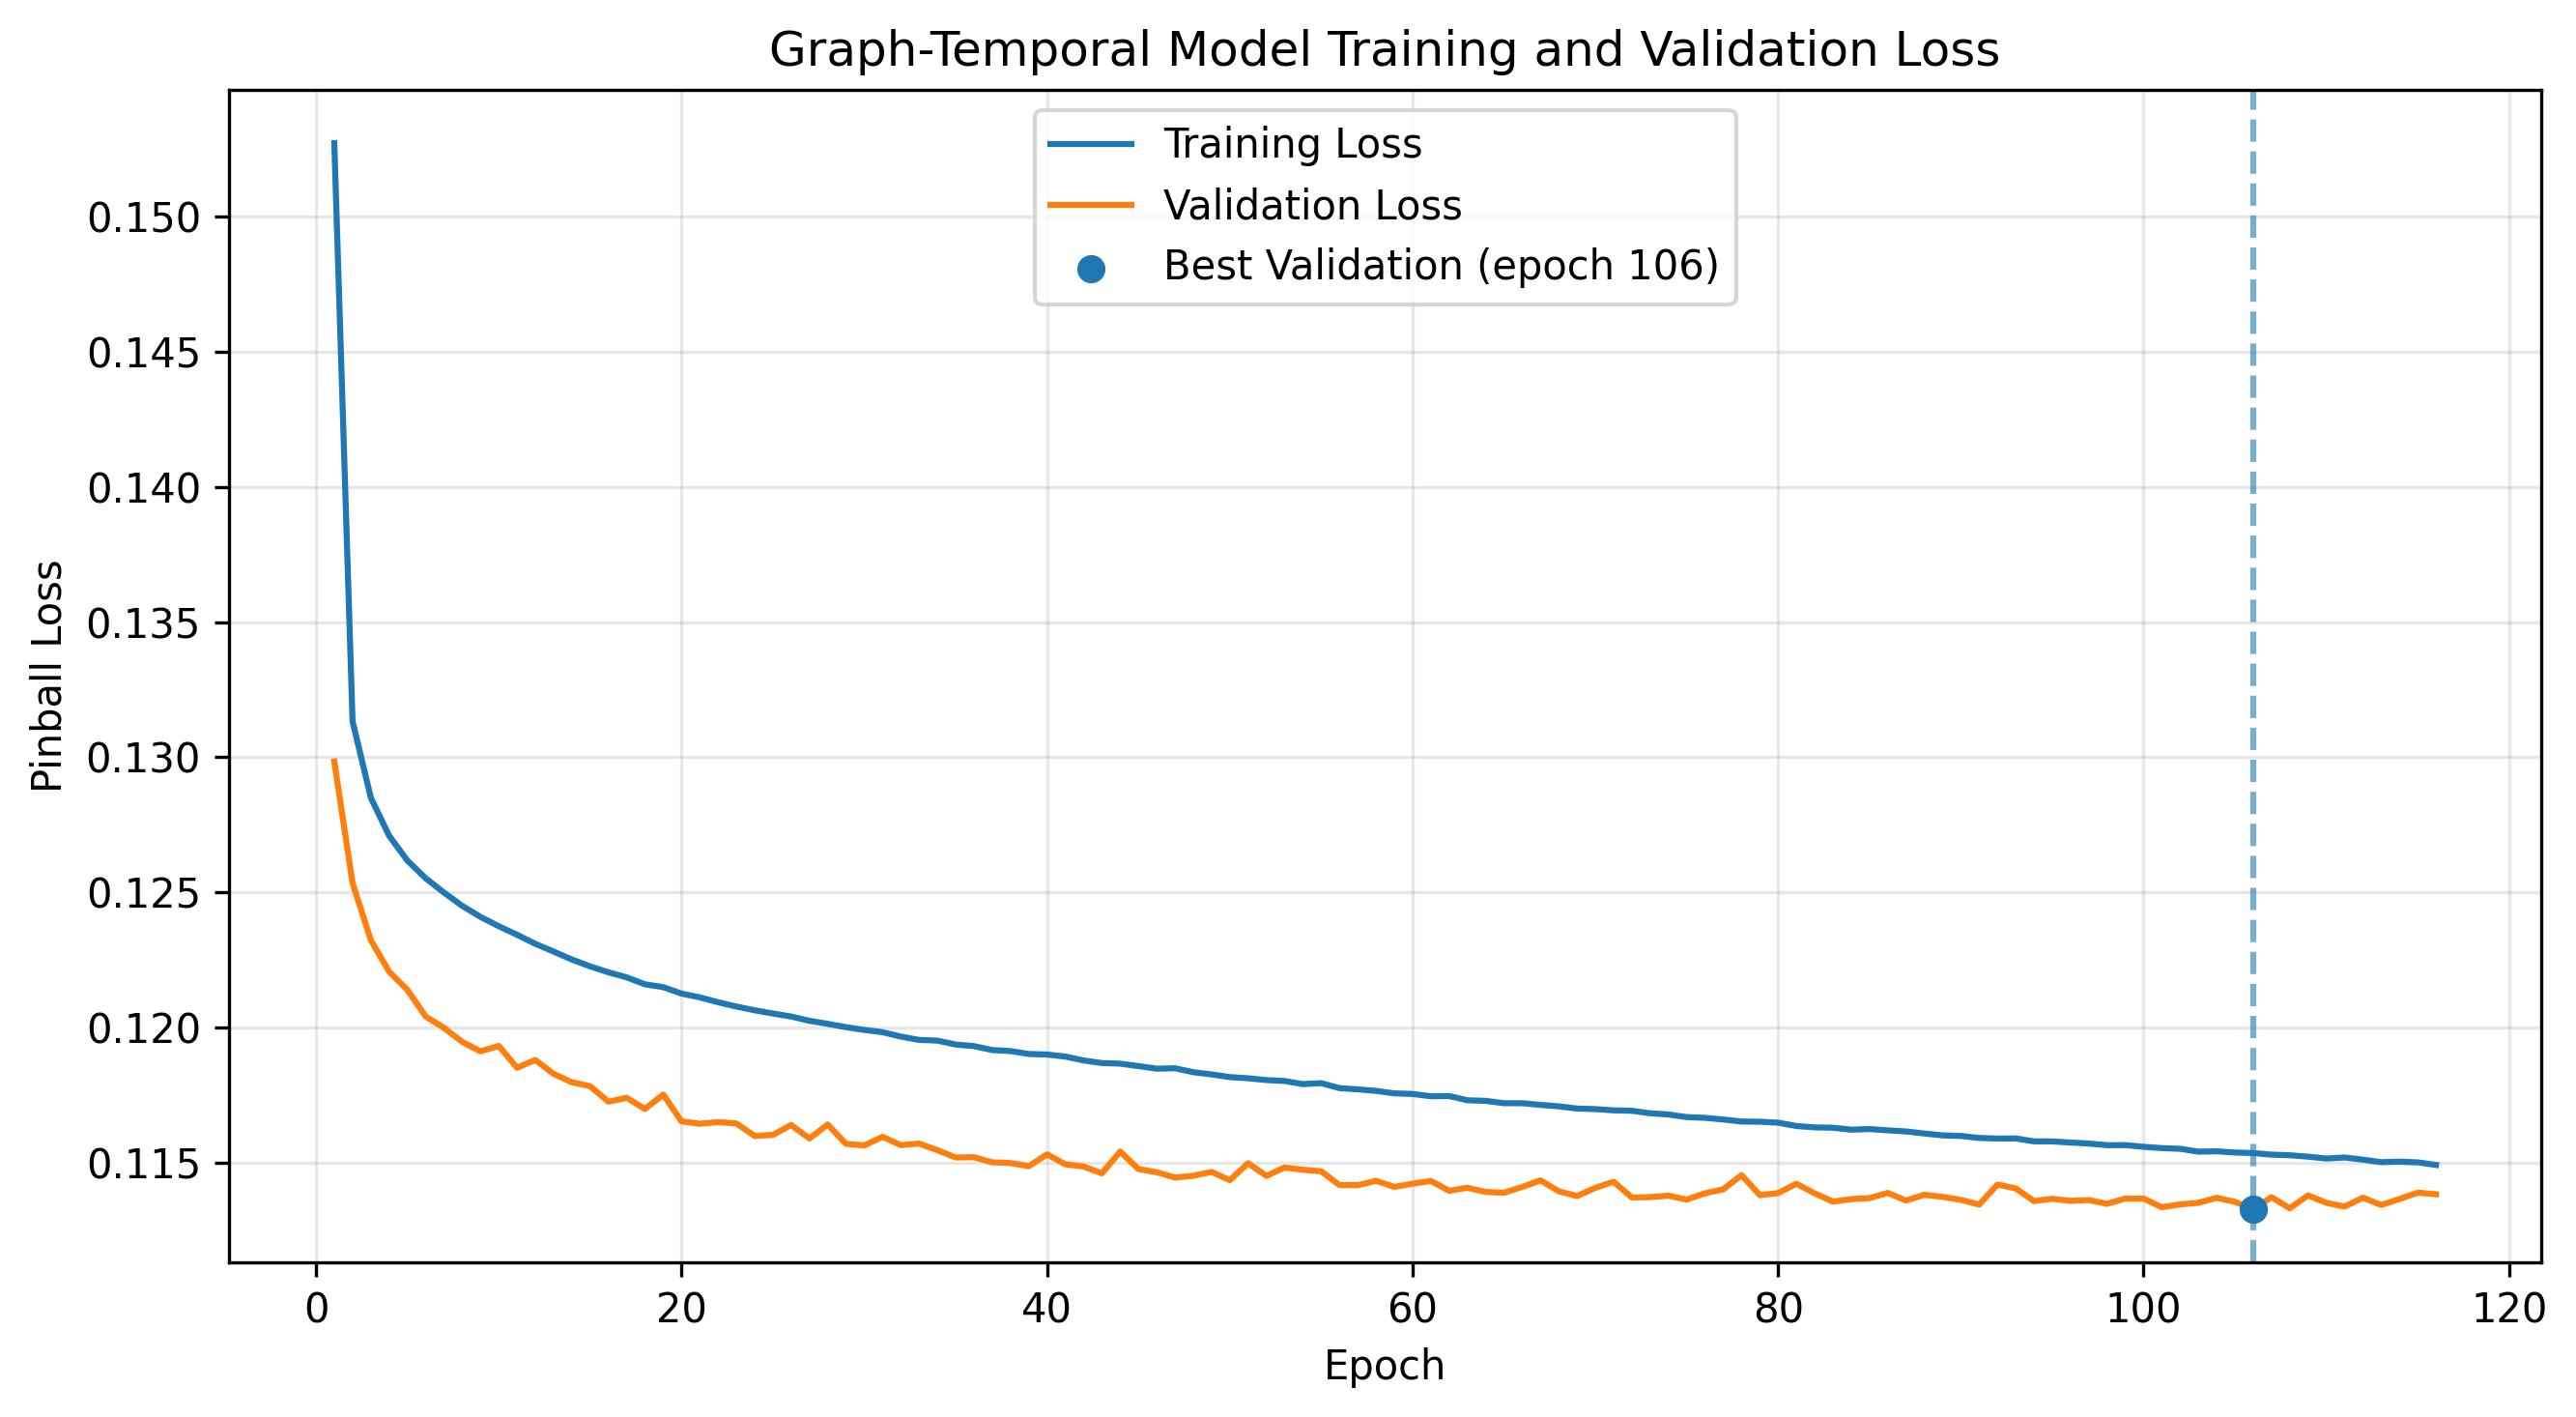
\includegraphics[width=\linewidth]{img/graph_temporal/graph_temporal_learning_curves}
        \caption{Graph-Temporal model.}
        \label{fig:graph_learning_curve}
    \end{subfigure}

    \caption{Training and validation Pinball Loss for the selected model
    configurations.}
    \label{fig:learning_curves}
\end{figure}

Validation Pinball Loss was used as the single model-selection criterion
rather than selecting configurations directly according to empirical
coverage. This criterion evaluates the quality of the predicted quantiles
without optimizing the model specifically for a single coverage statistic.
Coverage and interval width were instead retained as complementary
reliability metrics for the final analysis.


\subsection{Evaluation Metrics}
\label{subsec:metrics}

Performance is evaluated at the three forecasting horizons of 15, 30, and 60 minutes. All metrics are
computed only over valid target observations using the corresponding target
availability mask.

Point forecasting accuracy is evaluated using the median prediction
$\hat{y}^{(0.5)}$. The Mean Absolute Error (MAE) is defined as

\begin{equation}
    \mathrm{MAE}
    =
    \frac{1}{|\Omega|}
    \sum_{i\in\Omega}
    \left|
        y_i-\hat{y}^{(0.5)}_i
    \right|,
    \label{eq:mae}
\end{equation}

where $\Omega$ denotes the set of valid target entries at the considered
forecast horizon.

The Root Mean Squared Error (RMSE) is defined as

\begin{equation}
    \mathrm{RMSE}
    =
    \sqrt{
        \frac{1}{|\Omega|}
        \sum_{i\in\Omega}
        \left(
            y_i-\hat{y}^{(0.5)}_i
        \right)^2
    }.
    \label{eq:rmse}
\end{equation}

While MAE measures the average magnitude of the forecasting error, RMSE
assigns greater weight to large deviations and is therefore useful for
identifying models that occasionally produce particularly inaccurate
forecasts.

Probabilistic forecasting quality is evaluated through the Pinball Loss
introduced in Equation~\ref{eq:pinball_loss}. The loss is reported
separately for $q_{0.1}$, $q_{0.5}$, and $q_{0.9}$, allowing the quality of
the lower, median, and upper conditional quantile estimates to be examined
individually.

The reliability of the predictive intervals is assessed through empirical
coverage. For the nominal 80\% interval
$[\hat{y}^{(0.1)},\hat{y}^{(0.9)}]$, coverage is computed as

\begin{equation}
    \mathrm{Coverage}
    =
    \frac{1}{|\Omega|}
    \sum_{i\in\Omega}
    \mathbb{I}
    \left[
        \hat{y}^{(0.1)}_i
        \leq y_i
        \leq
        \hat{y}^{(0.9)}_i
    \right],
    \label{eq:coverage}
\end{equation}

where $\mathbb{I}[\cdot]$ is the indicator function. A well-calibrated
80\% predictive interval is expected to contain approximately 80\% of the
observed targets.

Coverage alone is not sufficient to characterize forecast quality, since
arbitrarily wide intervals could achieve high coverage. Predictive sharpness
is therefore evaluated using the mean interval width,

\begin{equation}
    \mathrm{Width}
    =
    \frac{1}{|\Omega|}
    \sum_{i\in\Omega}
    \left(
        \hat{y}^{(0.9)}_i
        -
        \hat{y}^{(0.1)}_i
    \right).
    \label{eq:interval_width}
\end{equation}

Coverage and interval width are interpreted jointly: reliable forecasts
should achieve coverage close to the nominal level while keeping predictive
intervals as informative as possible.

Finally, the quantile crossing rate measures the fraction of predictions for
which the estimated quantiles violate their expected ordering,

\begin{equation}
    \hat{y}^{(0.1)}
    \leq
    \hat{y}^{(0.5)}
    \leq
    \hat{y}^{(0.9)}.
\end{equation}

A crossing rate close to zero indicates that the independently predicted
quantiles are almost always ordered consistently.

In addition to these scalar metrics, calibration plots are used to compare
the nominal quantile levels with their empirical frequencies. This provides
a more detailed view of probabilistic calibration than the 80\% interval
coverage alone.


\subsection{Hardware and Reproducibility}
\label{subsec:hardware}

All neural models were implemented in PyTorch and trained using an NVIDIA
GeForce RTX 4060 Laptop GPU with CUDA acceleration. A fixed random seed of
42 was used throughout the experiments to improve reproducibility.

Model checkpoints corresponding to the best validation Pinball Loss were
saved during training and subsequently reloaded for final evaluation. The
same preprocessing pipeline, dataset partitions, forecast horizons, and
evaluation functions were used across the learned models to ensure a
consistent experimental comparison.

\section{In-Distribution Forecasting Results}
\label{sec:in_distribution_results}


\subsection{Point Forecasting Performance}
\label{subsec:point_results}

The point forecasting performance of the three models is reported in
Table~\ref{tab:point_results}. For the two probabilistic neural models, the
median prediction $q_{0.5}$ is used as the point forecast. As expected,
forecasting accuracy decreases as the prediction horizon increases, with
both MAE and RMSE increasing from 15 to 60 minutes for all models.

\begin{table}[t]
    \centering
    \caption{Point forecasting performance on the test set at the three
    forecasting horizons. The best result for each metric and horizon is
    highlighted in bold.}
    \label{tab:point_results}
    \begin{tabular}{llccc}
        \toprule
        & & \multicolumn{3}{c}{Forecast horizon} \\
        \cmidrule(lr){3-5}
        Model & Metric & 15 min & 30 min & 60 min \\
        \midrule

        Persistence
        & MAE  & 3.501 & 4.199 & 5.351 \\
        & RMSE & 6.411 & 8.023 & 10.279 \\
        \midrule

        Temporal GRU
        & MAE  & 3.080 & 3.735 & 4.733 \\
        & RMSE & 6.081 & 7.548 & 9.411 \\
        \midrule

        Graph-Temporal
        & MAE  & \textbf{2.901} & \textbf{3.442} & \textbf{4.244} \\
        & RMSE & \textbf{5.511} & \textbf{6.758} & \textbf{8.378} \\
        \bottomrule
    \end{tabular}
\end{table}

The Persistence baseline exhibits the largest errors at all forecasting
horizons. Introducing temporal modeling through the GRU consistently improves
over persistence, showing that the recent history contains temporal patterns
that cannot be captured by simply propagating the final input value into the
future.

The Graph-Temporal model further reduces both MAE and RMSE at every horizon.
Compared with the Temporal model, the MAE decreases from 3.080 to 2.901 at
15 minutes, from 3.735 to 3.442 at 30 minutes, and from 4.733 to 4.244 at
60 minutes. These correspond to relative reductions of approximately
5.8\%, 7.8\%, and 10.3\%, respectively. The corresponding RMSE reductions
are approximately 9.4\%, 10.5\%, and 11.0\%.

The improvement introduced by the graph component becomes more pronounced
as the forecasting horizon increases. This suggests that spatial information
is particularly useful for longer-term predictions, where the future state
of a sensor becomes increasingly difficult to estimate from its own temporal
history alone. The reduction in RMSE is also consistently larger than the
reduction in MAE, indicating that the Graph-Temporal model is particularly
effective in reducing larger forecasting errors.

The same trend is illustrated in
Figure~\ref{fig:point_performance}, where the performance gap between the
Temporal model and the Graph-Temporal model becomes progressively larger toward
the 60-minute horizon.

\begin{figure}[t]
    \centering

    \begin{minipage}[b]{0.48\linewidth}
        \centering
        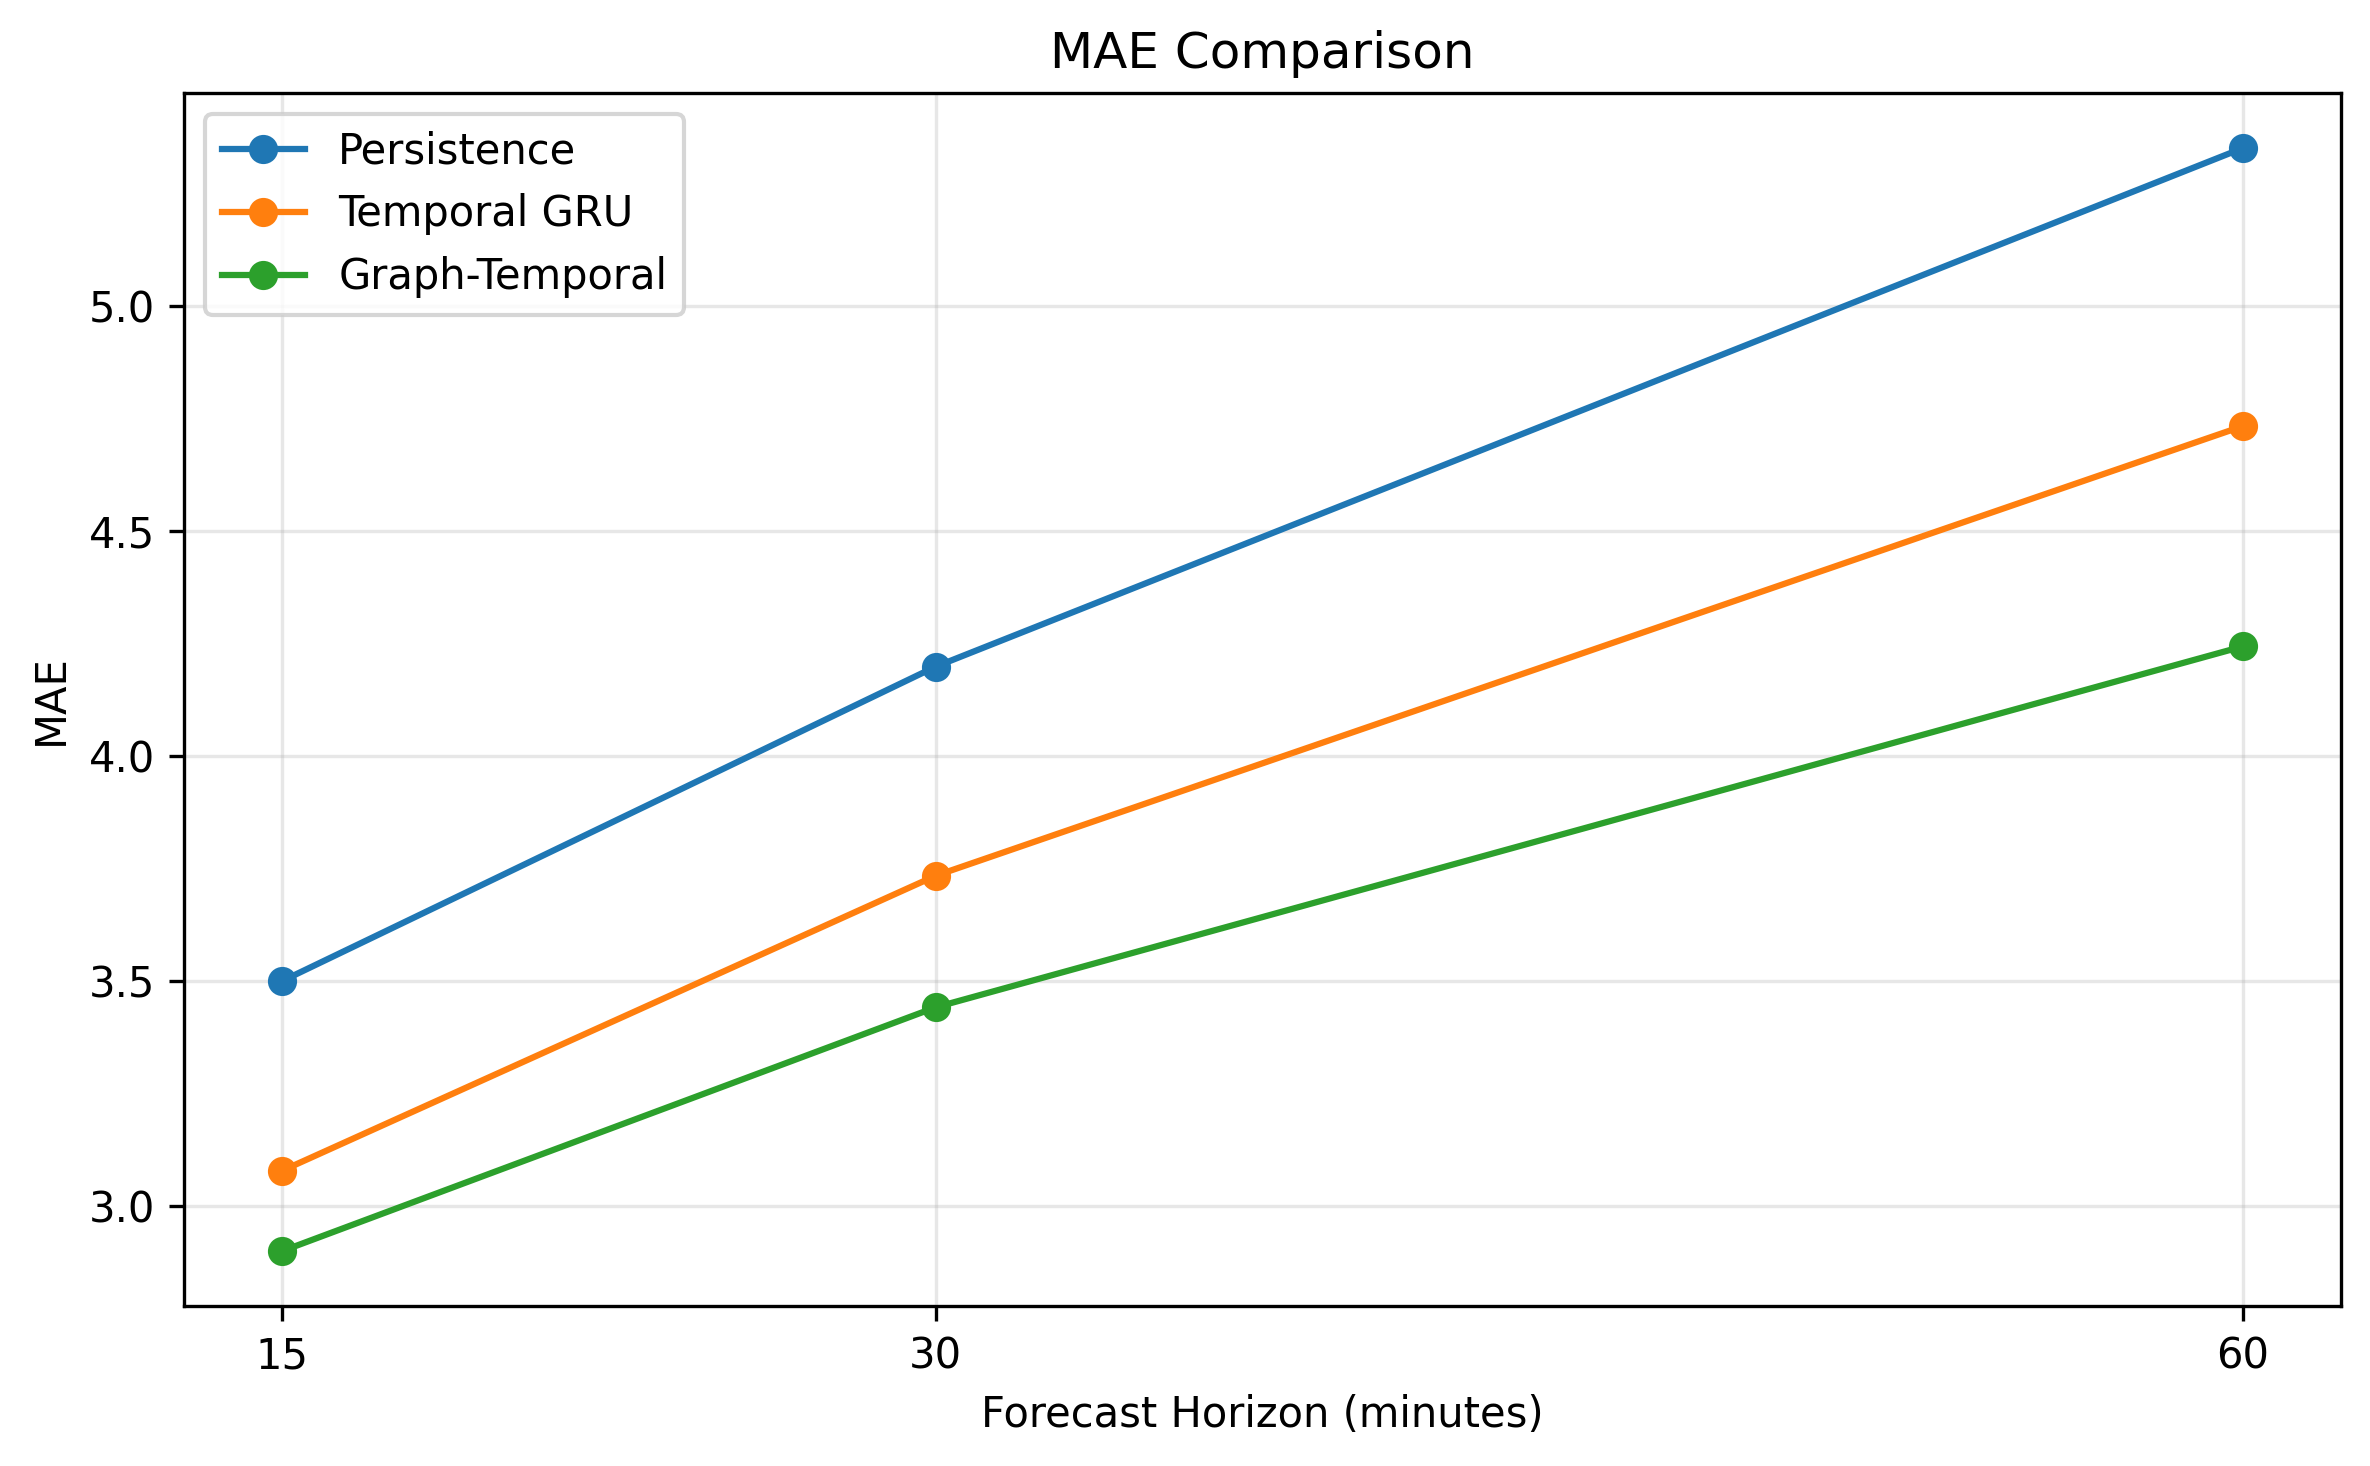
\includegraphics[width=\linewidth]{img/model_comparison/mae_model_comparison}
    \end{minipage}
    \hfill
    \begin{minipage}[b]{0.48\linewidth}
        \centering
        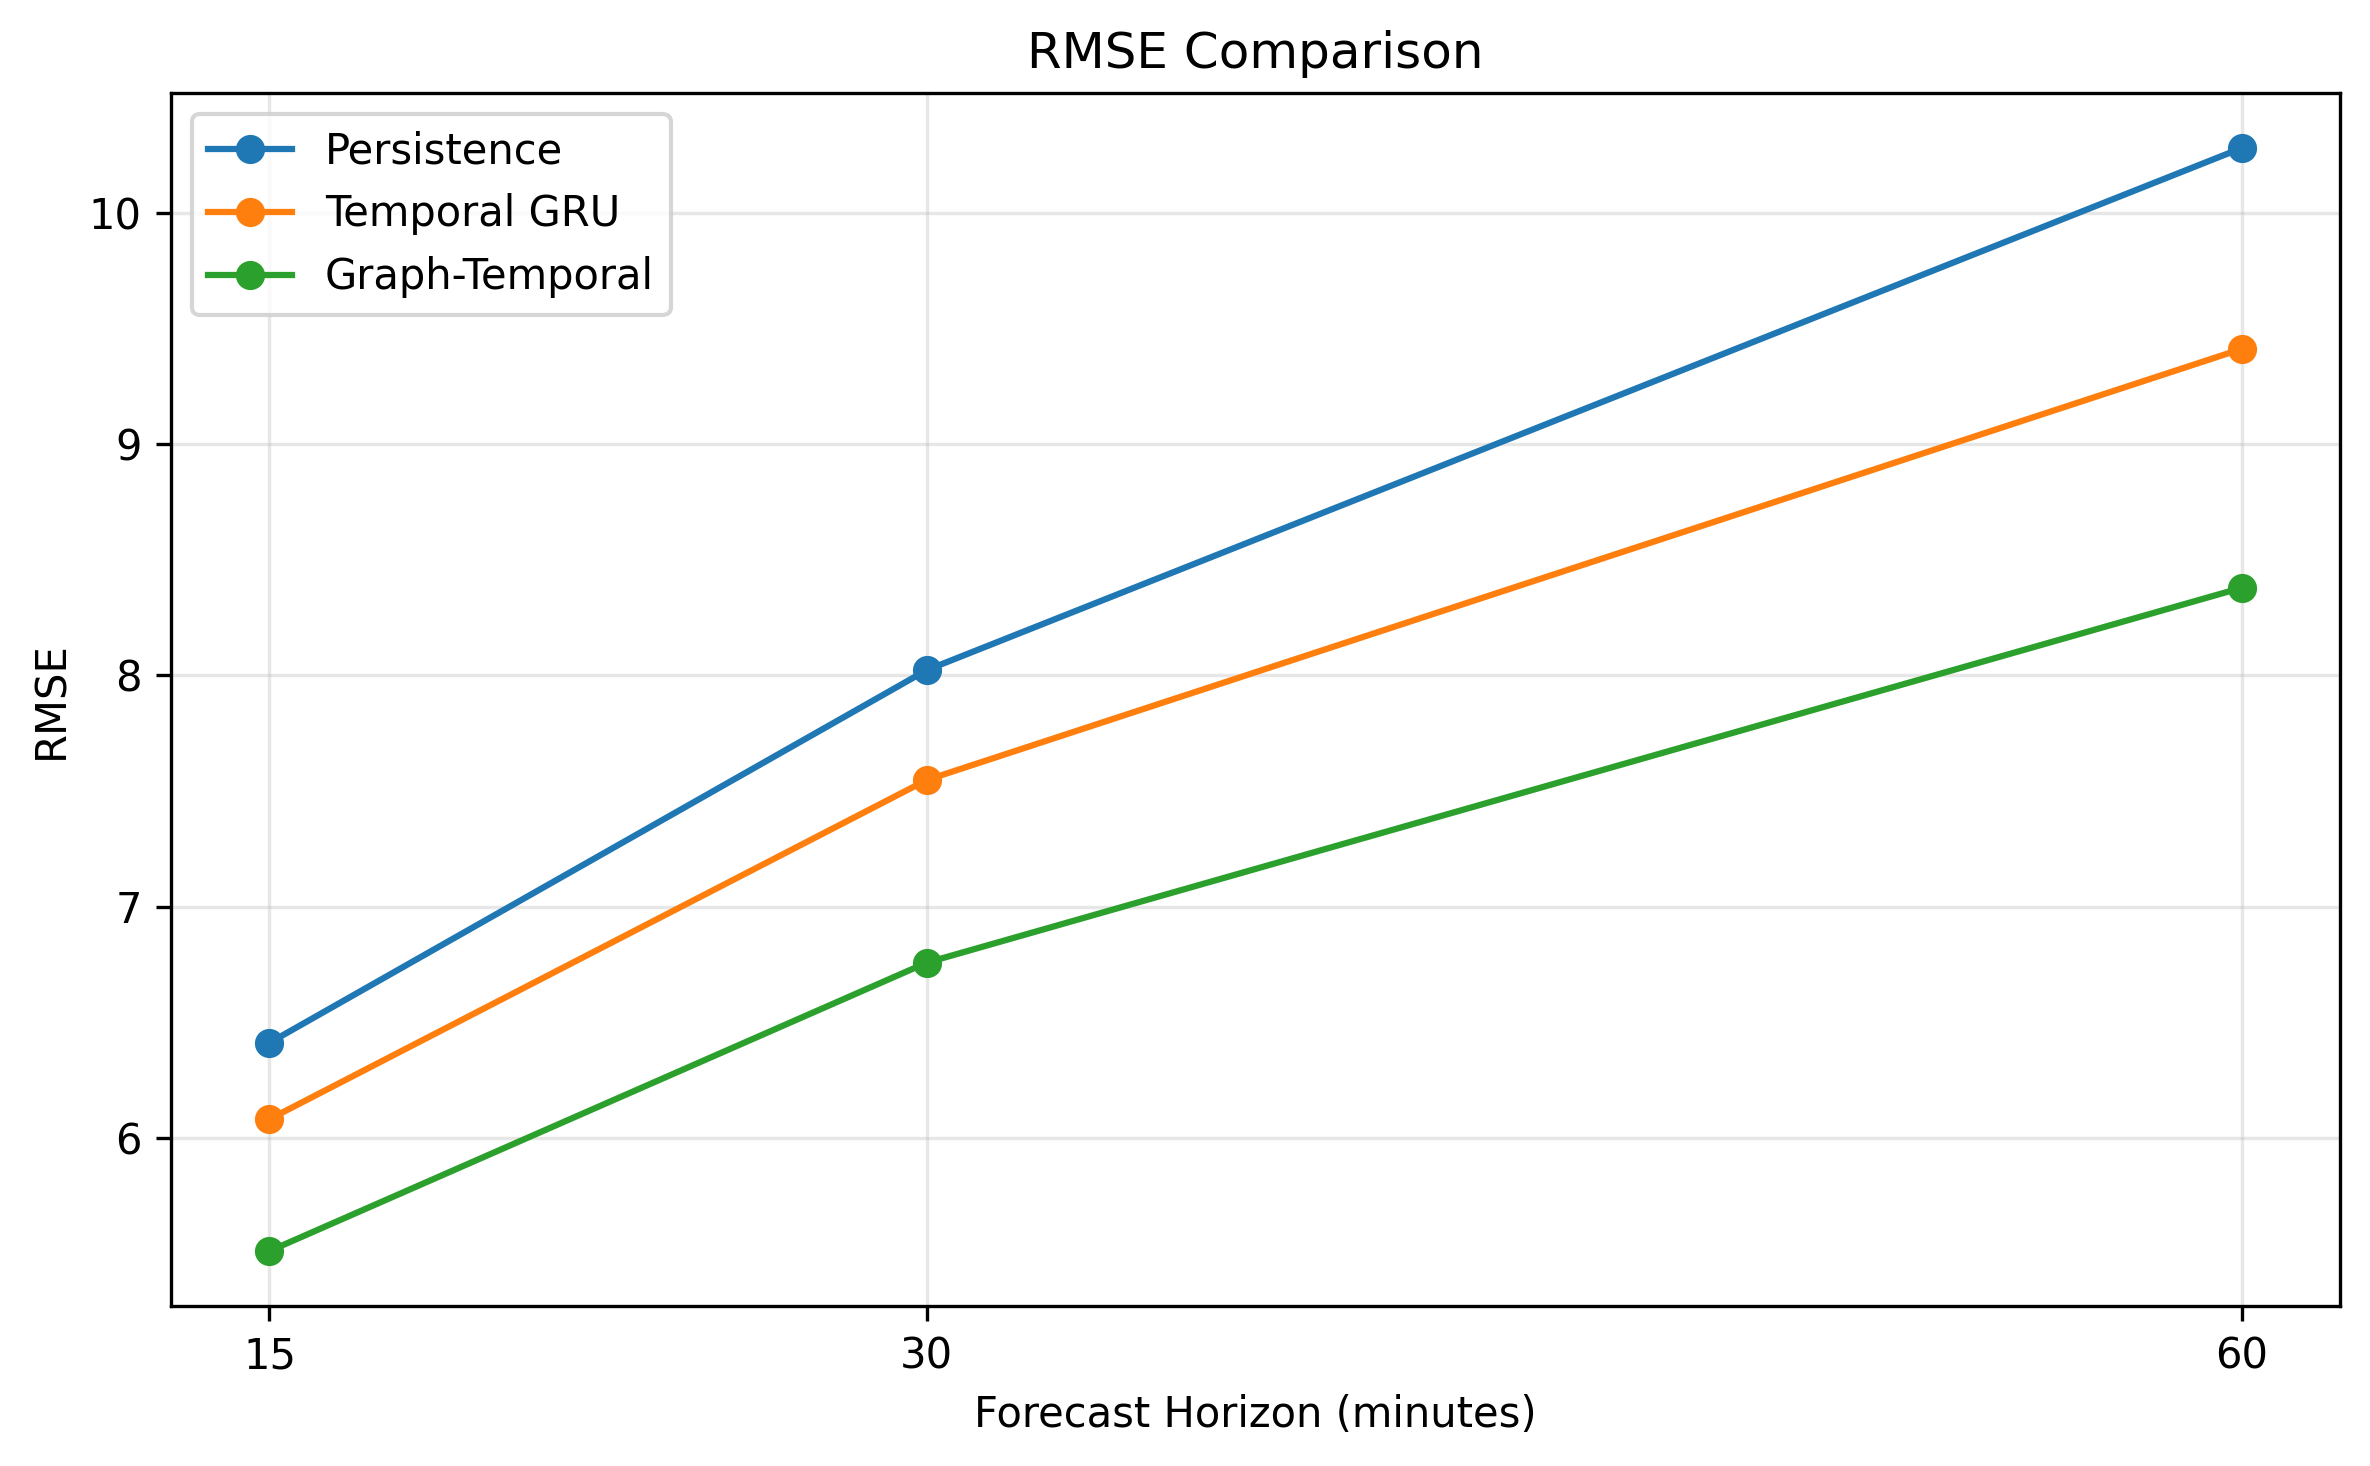
\includegraphics[width=\linewidth]{img/model_comparison/rmse_model_comparison}
    \end{minipage}

    \caption{Point forecasting performance of the Persistence, Temporal,
    and Graph-Temporal models across the three forecasting horizons in terms
    of MAE (left) and RMSE (right).}
    \label{fig:point_performance}
\end{figure}



\subsection{Probabilistic Forecasting and Calibration}
\label{subsec:probabilistic_results}

The probabilistic forecasting performance of the Temporal GRU and
Graph-Temporal models is reported in Table~\ref{tab:probabilistic_results}.
The Pinball Loss is evaluated separately for the three predicted quantiles,
while empirical coverage and interval width are used to assess the reliability
and sharpness of the nominal 80\% prediction intervals.

Across all forecasting horizons, the Graph-Temporal model achieves lower
Pinball Loss for each of the three quantiles. At 15 minutes, the losses for
$q_{0.1}$, $q_{0.5}$, and $q_{0.9}$ decrease from 0.952, 1.540, and 0.643
for the Temporal GRU to 0.845, 1.451, and 0.597 for the Graph-Temporal
model. The same behavior is observed at 30 and 60 minutes, indicating that
the benefit of incorporating spatial information is not limited to the
median forecast, but also extends to the estimation of the lower and upper
quantiles.

The two models, however, exhibit a different trade-off between calibration
and sharpness. The Temporal model achieves empirical coverage close to the
nominal 80\% level, with values of 81.30\%, 80.16\%, and 79.81\% at 15,
30, and 60 minutes, respectively. The Graph-Temporal model produces narrower
prediction intervals at every horizon, reducing the average interval width
from 9.339 to 8.929 at 15 minutes, from 10.931 to 10.485 at 30 minutes, and
from 13.309 to 12.470 at 60 minutes. This increased sharpness is accompanied
by slightly lower coverage, which remains between 78.13\% and 78.44\% across
the three horizons.

These results show that the Graph-Temporal model improves the quality of all
three estimated quantiles and produces more concentrated predictive
intervals, but the resulting intervals exhibit mild undercoverage relative
to the nominal 80\% level. In contrast, the Temporal model remains closer to
the nominal coverage overall, although it exhibits mild overcoverage at the
15-minute horizon, reaching 81.30\%.
The reliability-sharpness trade-off is further illustrated in
Figure~\ref{fig:probabilistic_comparison}.
Moreover, interval width increases with the
forecasting horizon for both models, reflecting the greater uncertainty of
longer-term predictions. The calibration behavior of the selected
Graph-Temporal model is further investigated under distribution shift in
Section~\ref{sec:distribution_shift}.

\begin{table}[t]
    \centering
    \caption{Probabilistic forecasting performance on the test set. Coverage
    refers to the nominal 80\% prediction interval defined by
    $q_{0.1}$ and $q_{0.9}$.}
    \label{tab:probabilistic_results}
    \resizebox{\linewidth}{!}{
    \begin{tabular}{llccccc}
        \toprule
        Model & Horizon
        & Pinball $q_{0.1}$
        & Pinball $q_{0.5}$
        & Pinball $q_{0.9}$
        & Coverage (\%)
        & Interval Width \\
        \midrule

        Temporal GRU
        & 15 min & 0.952 & 1.540 & 0.643 & 81.30 & 9.339 \\
        & 30 min & 1.225 & 1.867 & 0.743 & 80.16 & 10.931 \\
        & 60 min & 1.668 & 2.367 & 0.832 & 79.81 & 13.309 \\
        \midrule

        Graph-Temporal
        & 15 min & \textbf{0.845} & \textbf{1.451} & \textbf{0.597}
        & 78.44 & \textbf{8.929} \\
        & 30 min & \textbf{1.028} & \textbf{1.721} & \textbf{0.677}
        & 78.22 & \textbf{10.485} \\
        & 60 min & \textbf{1.320} & \textbf{2.122} & \textbf{0.775}
        & 78.13 & \textbf{12.470} \\
        \bottomrule
    \end{tabular}
    }
\end{table}

\begin{figure}[t]
    \centering

    \begin{minipage}[b]{0.49\linewidth}
        \centering
        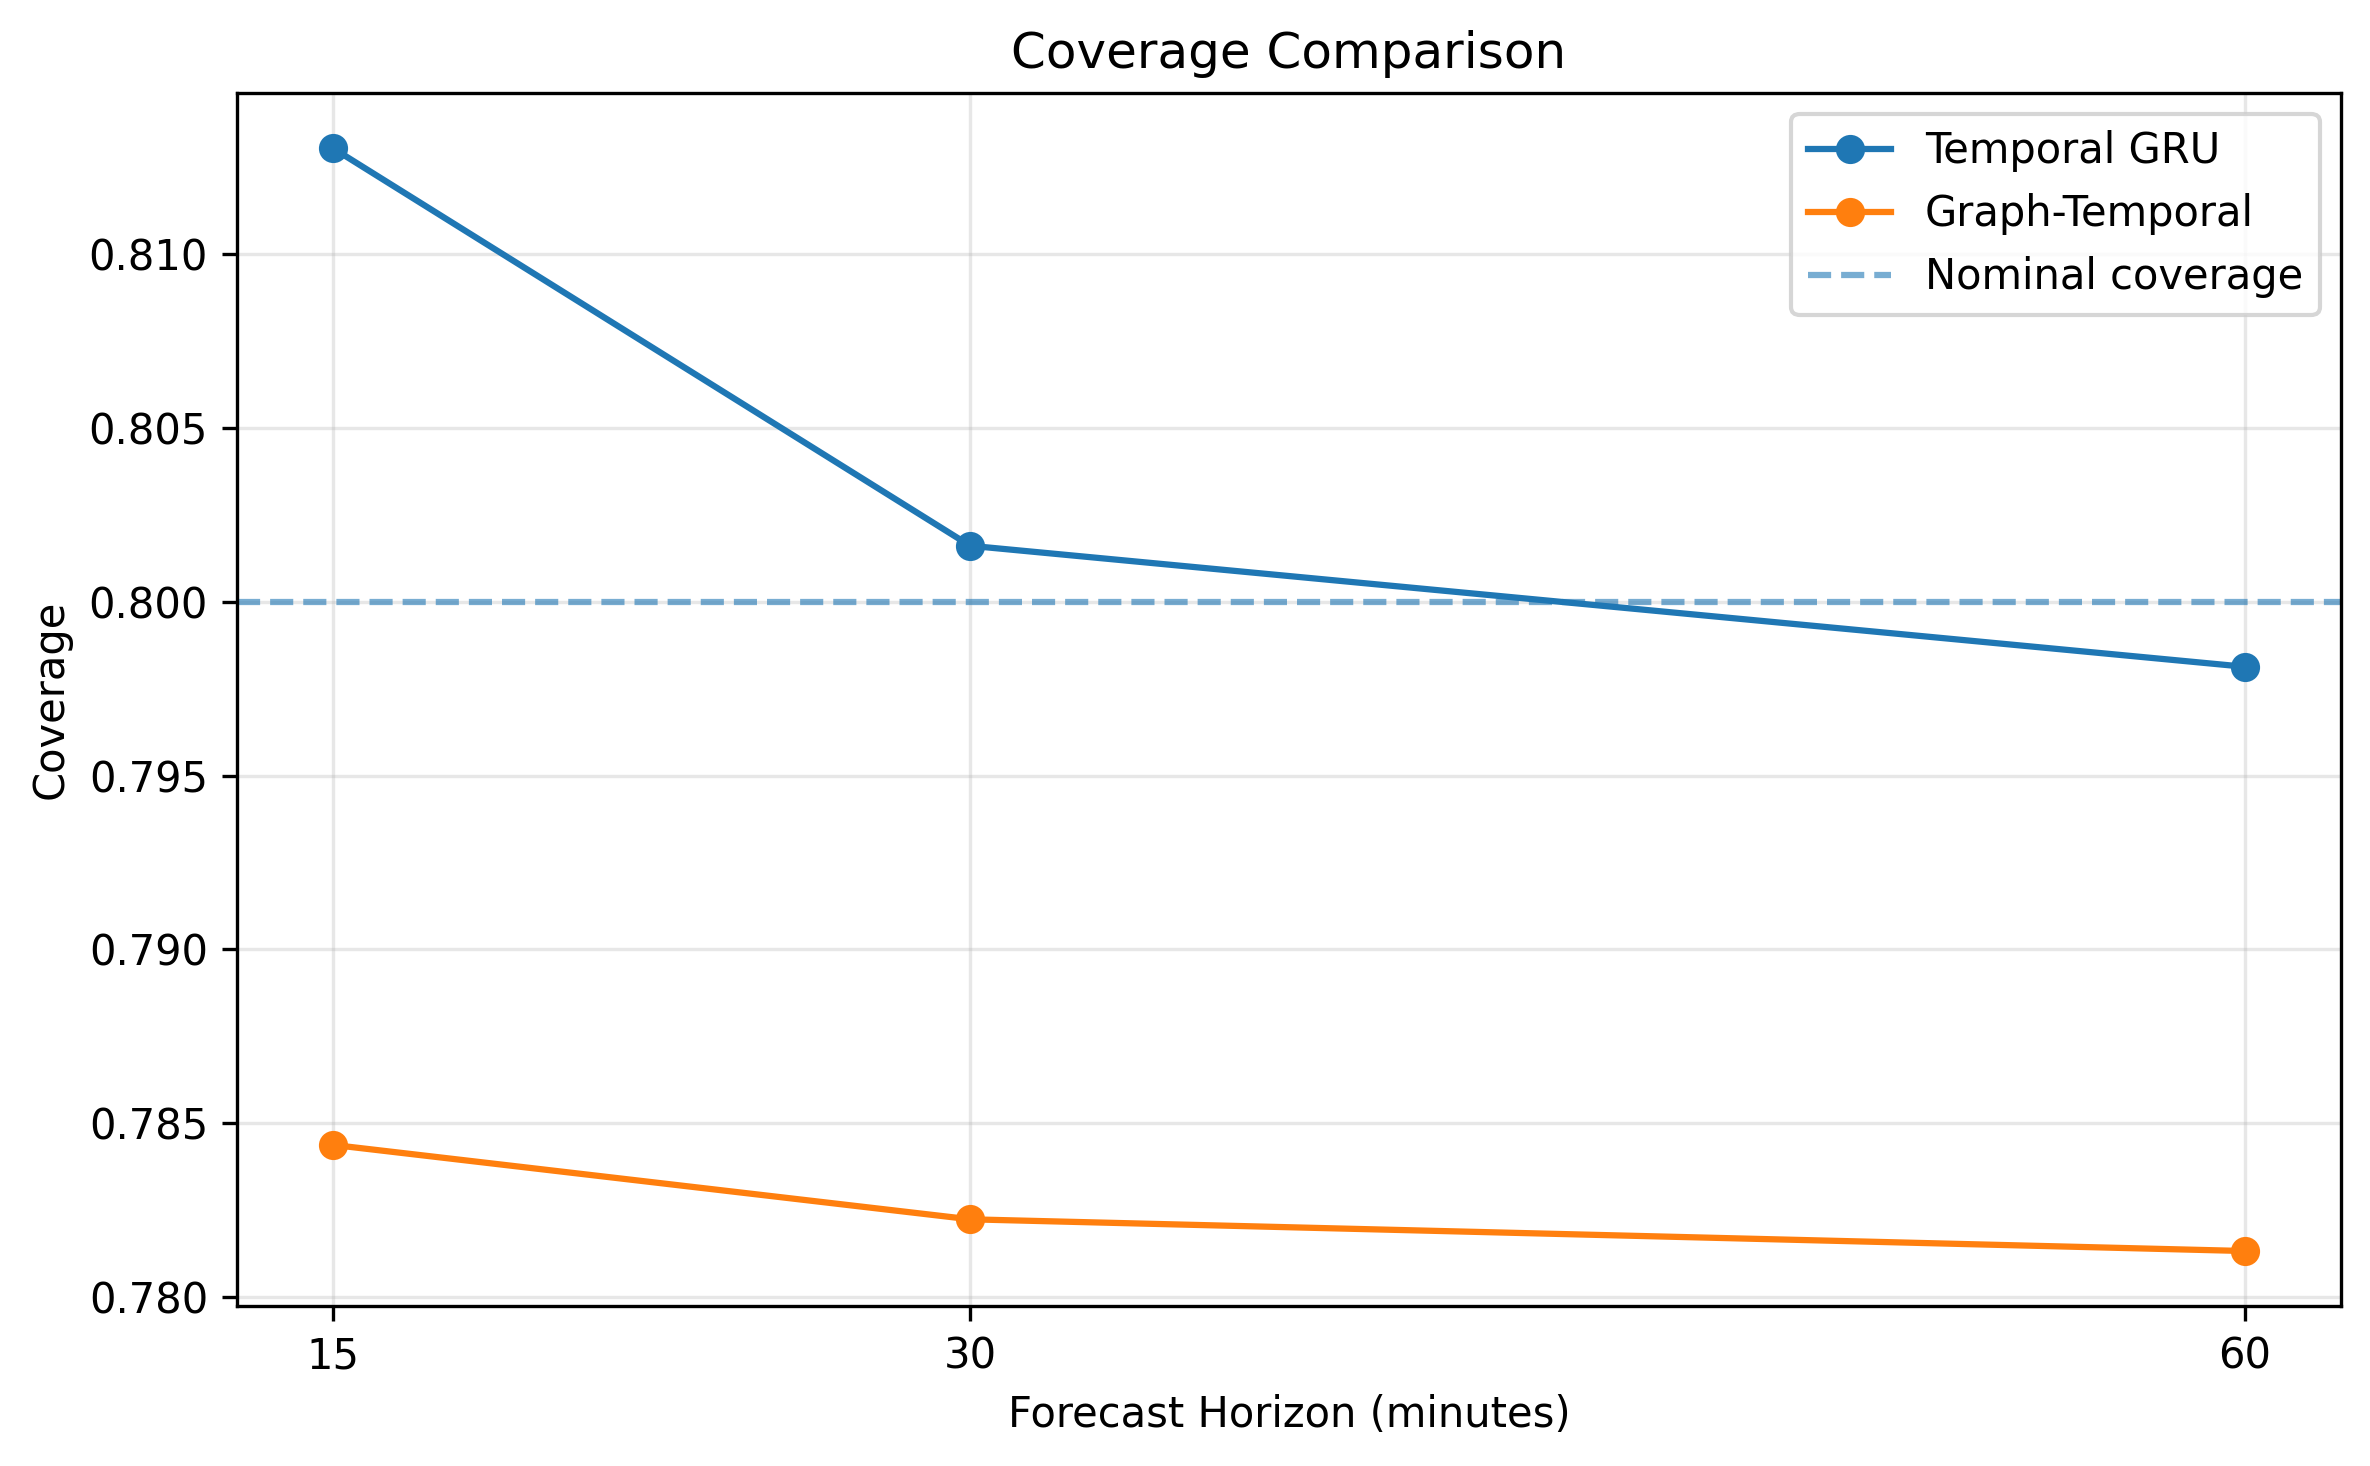
\includegraphics[width=\linewidth]{img/model_comparison/coverage_model_comparison}
    \end{minipage}
    \hfill
    \begin{minipage}[b]{0.49\linewidth}
        \centering
        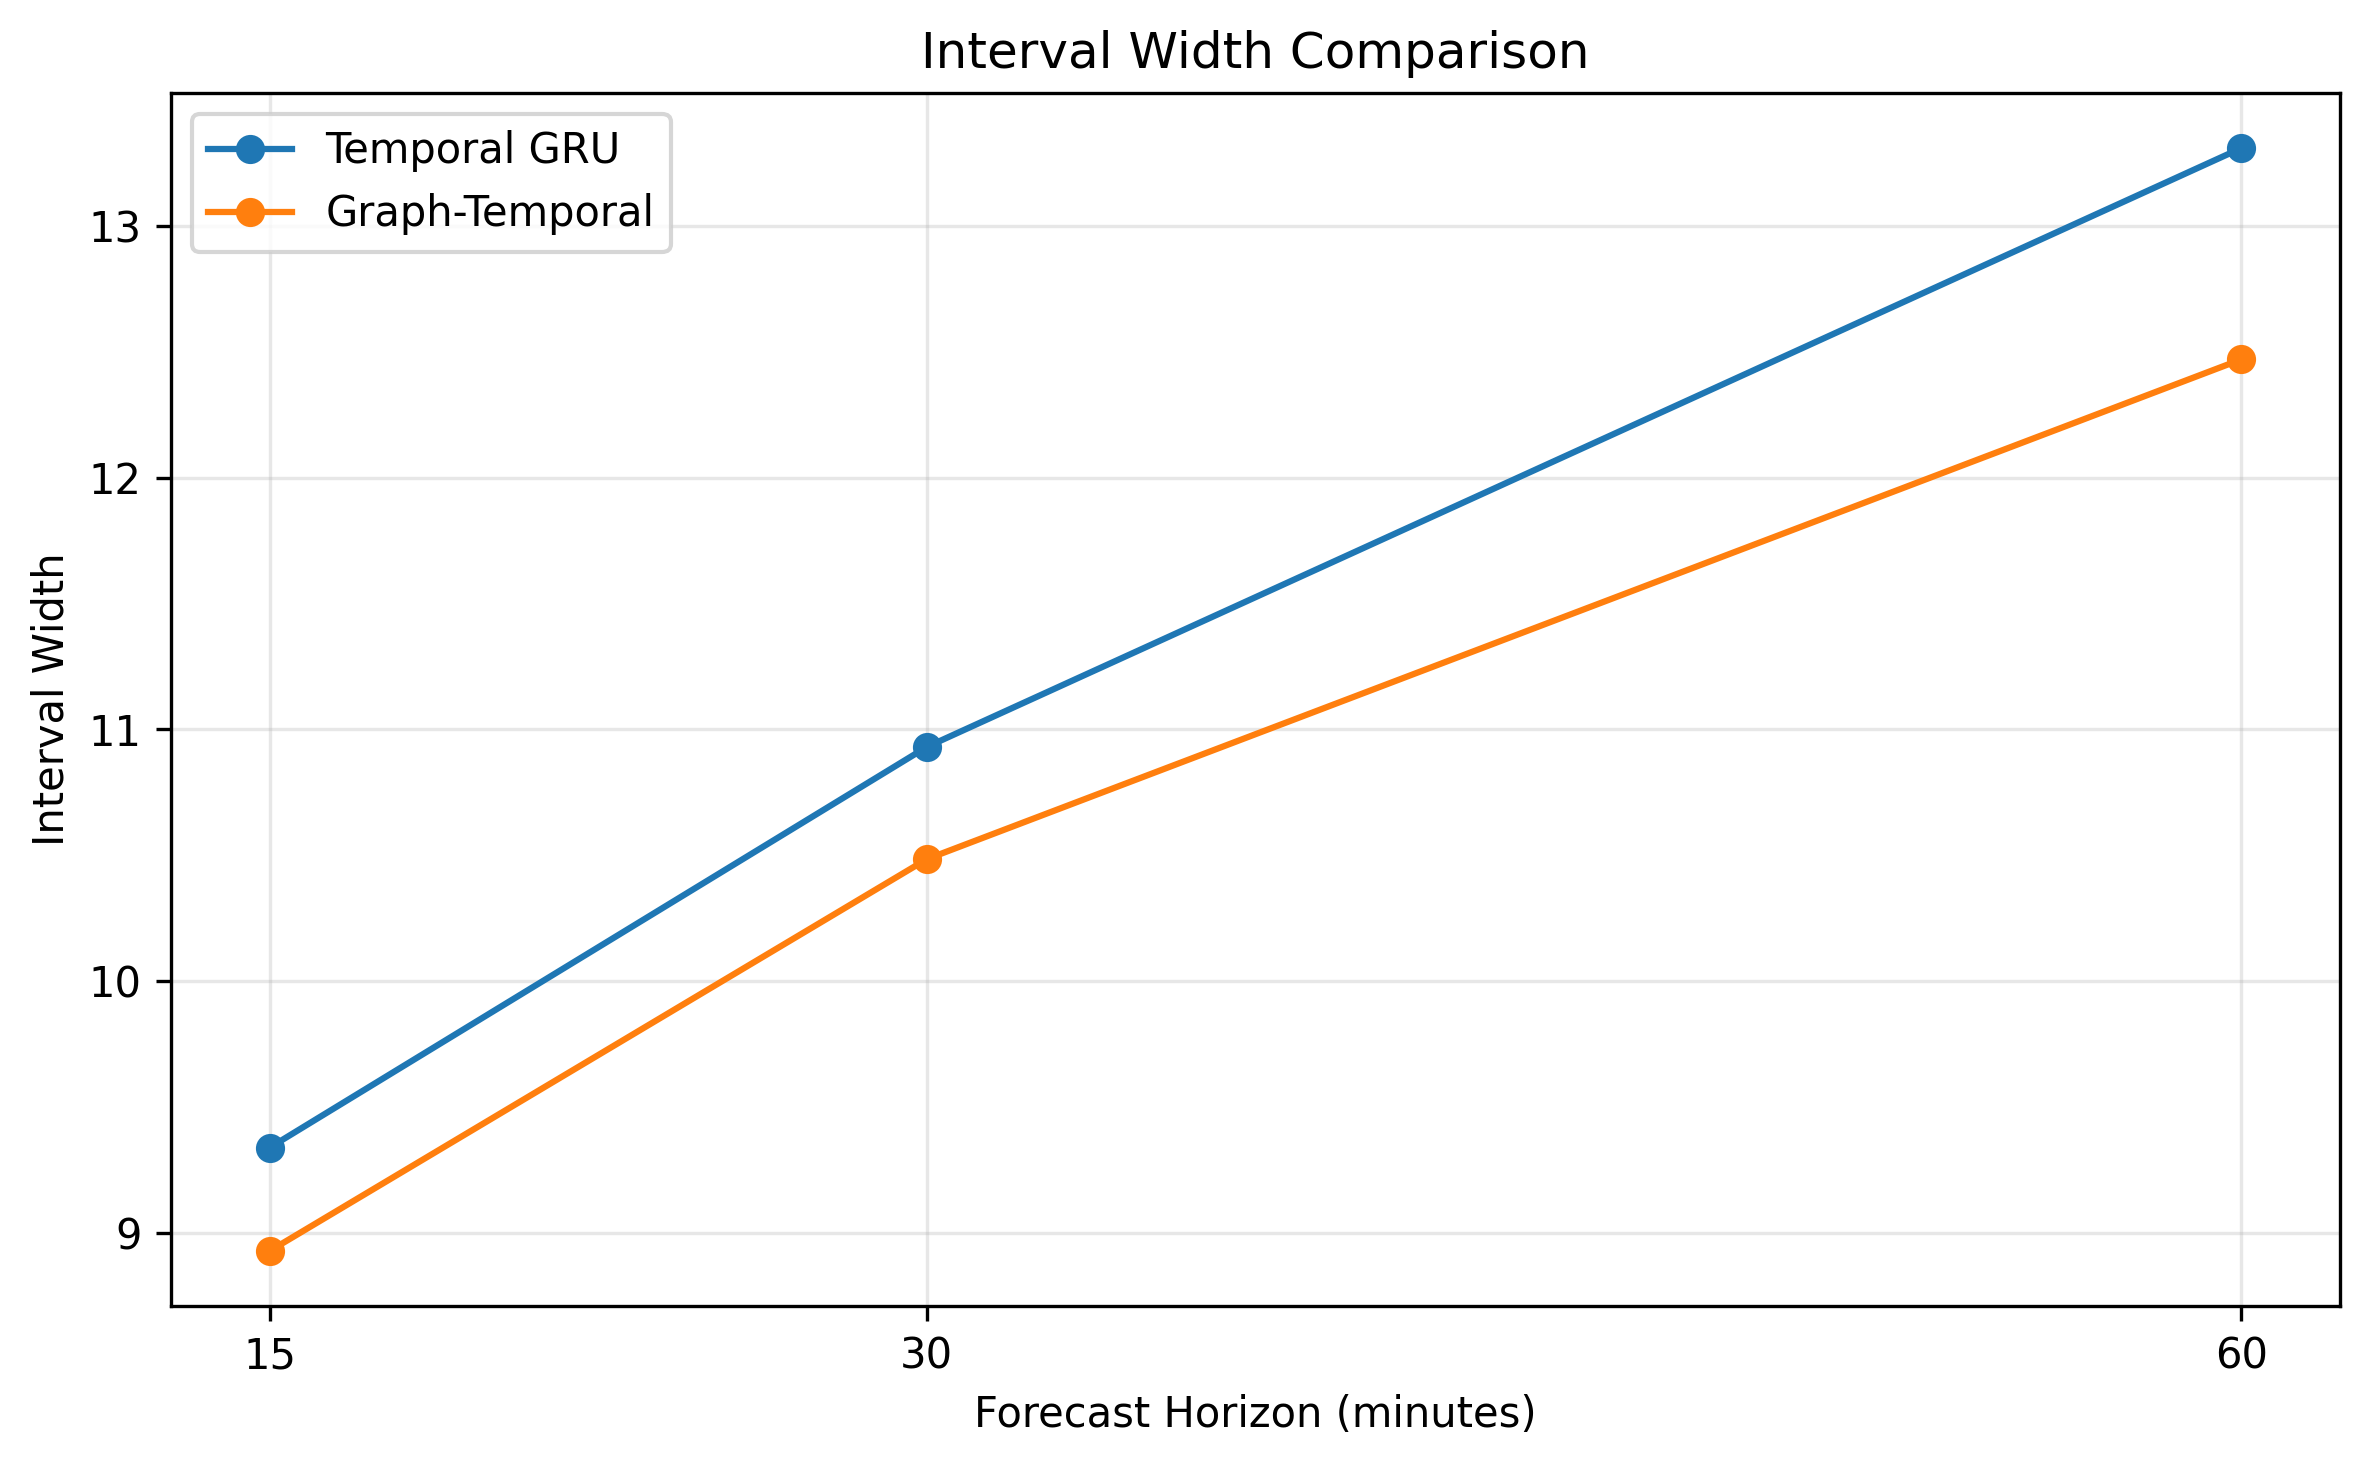
\includegraphics[width=\linewidth]{img/model_comparison/interval_width_model_comparison}
    \end{minipage}

    \caption{Comparison of the probabilistic forecasts produced by the
    Temporal GRU and Graph-Temporal models in terms of empirical coverage
    (left) and prediction interval width (right) across the three forecasting
    horizons. The dashed line in the coverage plot represents the nominal
    80\% coverage level.}
    \label{fig:probabilistic_comparison}
\end{figure}

Quantile crossing is negligible for both models, with rates below 0.05\%
at every forecasting horizon, indicating that the predicted quantiles
almost always preserve their expected ordering.

A more detailed view of probabilistic reliability is provided by the
calibration curves in Figure~\ref{fig:quantile_calibration}. The plots compare the
nominal quantile levels with their empirical frequencies and complement the
interval-level coverage results reported in
Table~\ref{tab:probabilistic_results}.

\begin{figure}[t]
    \centering

    \begin{minipage}[b]{0.49\linewidth}
        \centering
        
\includegraphics[width=\linewidth]{img/temporal_gru/calibration_plot}
    \end{minipage}
    \hfill
    \begin{minipage}[b]{0.49\linewidth}
        \centering
        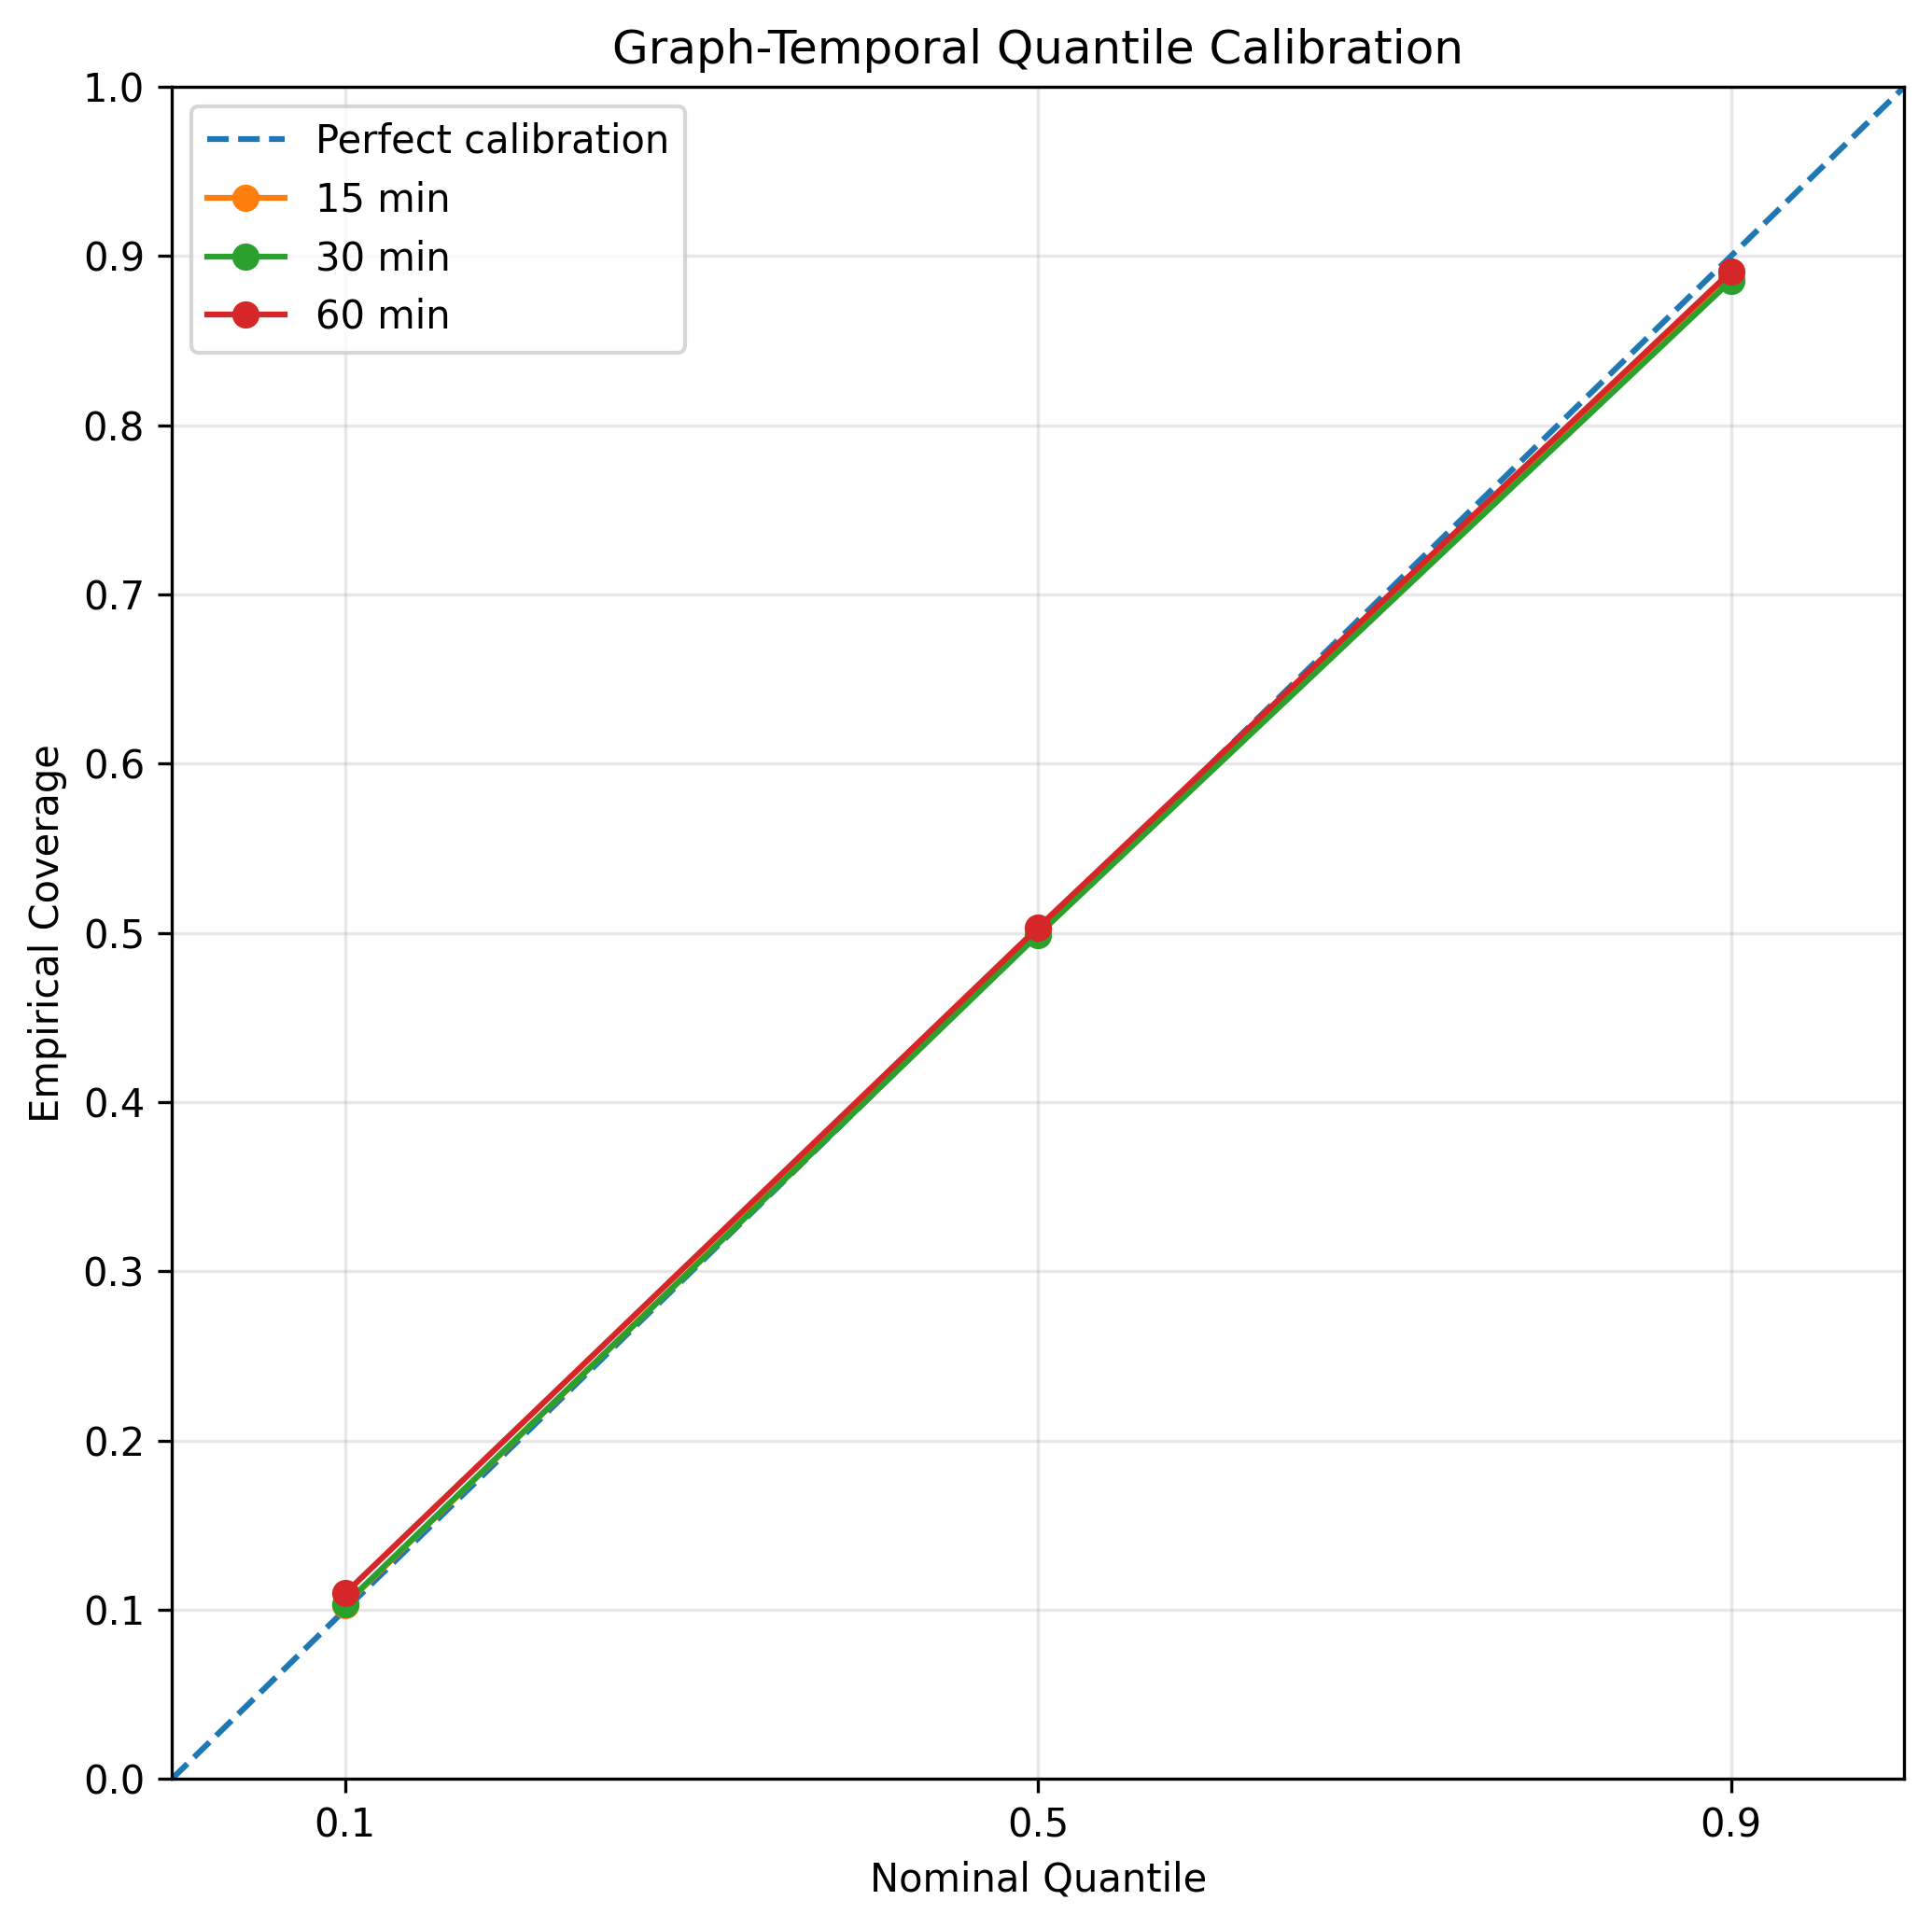
\includegraphics[width=\linewidth]{img/graph_temporal/calibration_plot}
    \end{minipage}

    \caption{Quantile calibration of the Temporal (left) and
    Graph-Temporal (right) models at the three forecasting horizons.
    The dashed diagonal represents perfect calibration.}
    \label{fig:quantile_calibration}
\end{figure}

\section{Analysis of the Graph Component}
\label{sec:graph_analysis}

\subsection{When Does the Graph Help?}
\label{subsec:graph_effect}

The aggregate results presented in Section~\ref{sec:in_distribution_results}
show that incorporating graph information improves forecasting accuracy at
all three horizons. To determine whether this improvement is widespread
across the road network or concentrated on a limited subset of sensors, the
two neural models were additionally compared at sensor level.

For each sensor $n$ and forecasting horizon $h$, the effect of graph message
passing is quantified as the difference between the MAE of the Temporal
and that of the Graph-Temporal model,

\begin{equation}
    \Delta \mathrm{MAE}_{n,h}
    =
    \mathrm{MAE}^{\mathrm{Temporal}}_{n,h}
    -
    \mathrm{MAE}^{\mathrm{Graph}}_{n,h}.
    \label{eq:delta_mae}
\end{equation}

A positive value of $\Delta \mathrm{MAE}_{n,h}$ therefore indicates that
incorporating graph information reduces the forecasting error for sensor
$n$, whereas a negative value indicates that the Temporal model performs
better for that sensor.

The sensor-level comparison shows that the aggregate improvement is not
driven by only a small subset of locations. The Graph-Temporal model reduces
MAE for 199 out of 207 sensors at the 15-minute horizon and for 200 out of
207 sensors at 30 minutes. At 60 minutes, graph message passing remains
beneficial for 193 out of 207 sensors. Therefore, the advantage observed in
the aggregate metrics is distributed across the large majority of the sensor
network, although a small number of locations consistently or occasionally
benefit more from purely temporal modeling.

To complement the sensor-level aggregate analysis, representative forecasting
examples are examined in Figure~\ref{fig:graph_help_examples}. The examples
compare the predictions of the Temporal and Graph-Temporal models for
sensor-time pairs in which the inclusion of spatial information produces a
clear reduction in forecasting error.

\begin{figure}[t]
    \centering

    \begin{minipage}[b]{0.8\linewidth}
        \centering
        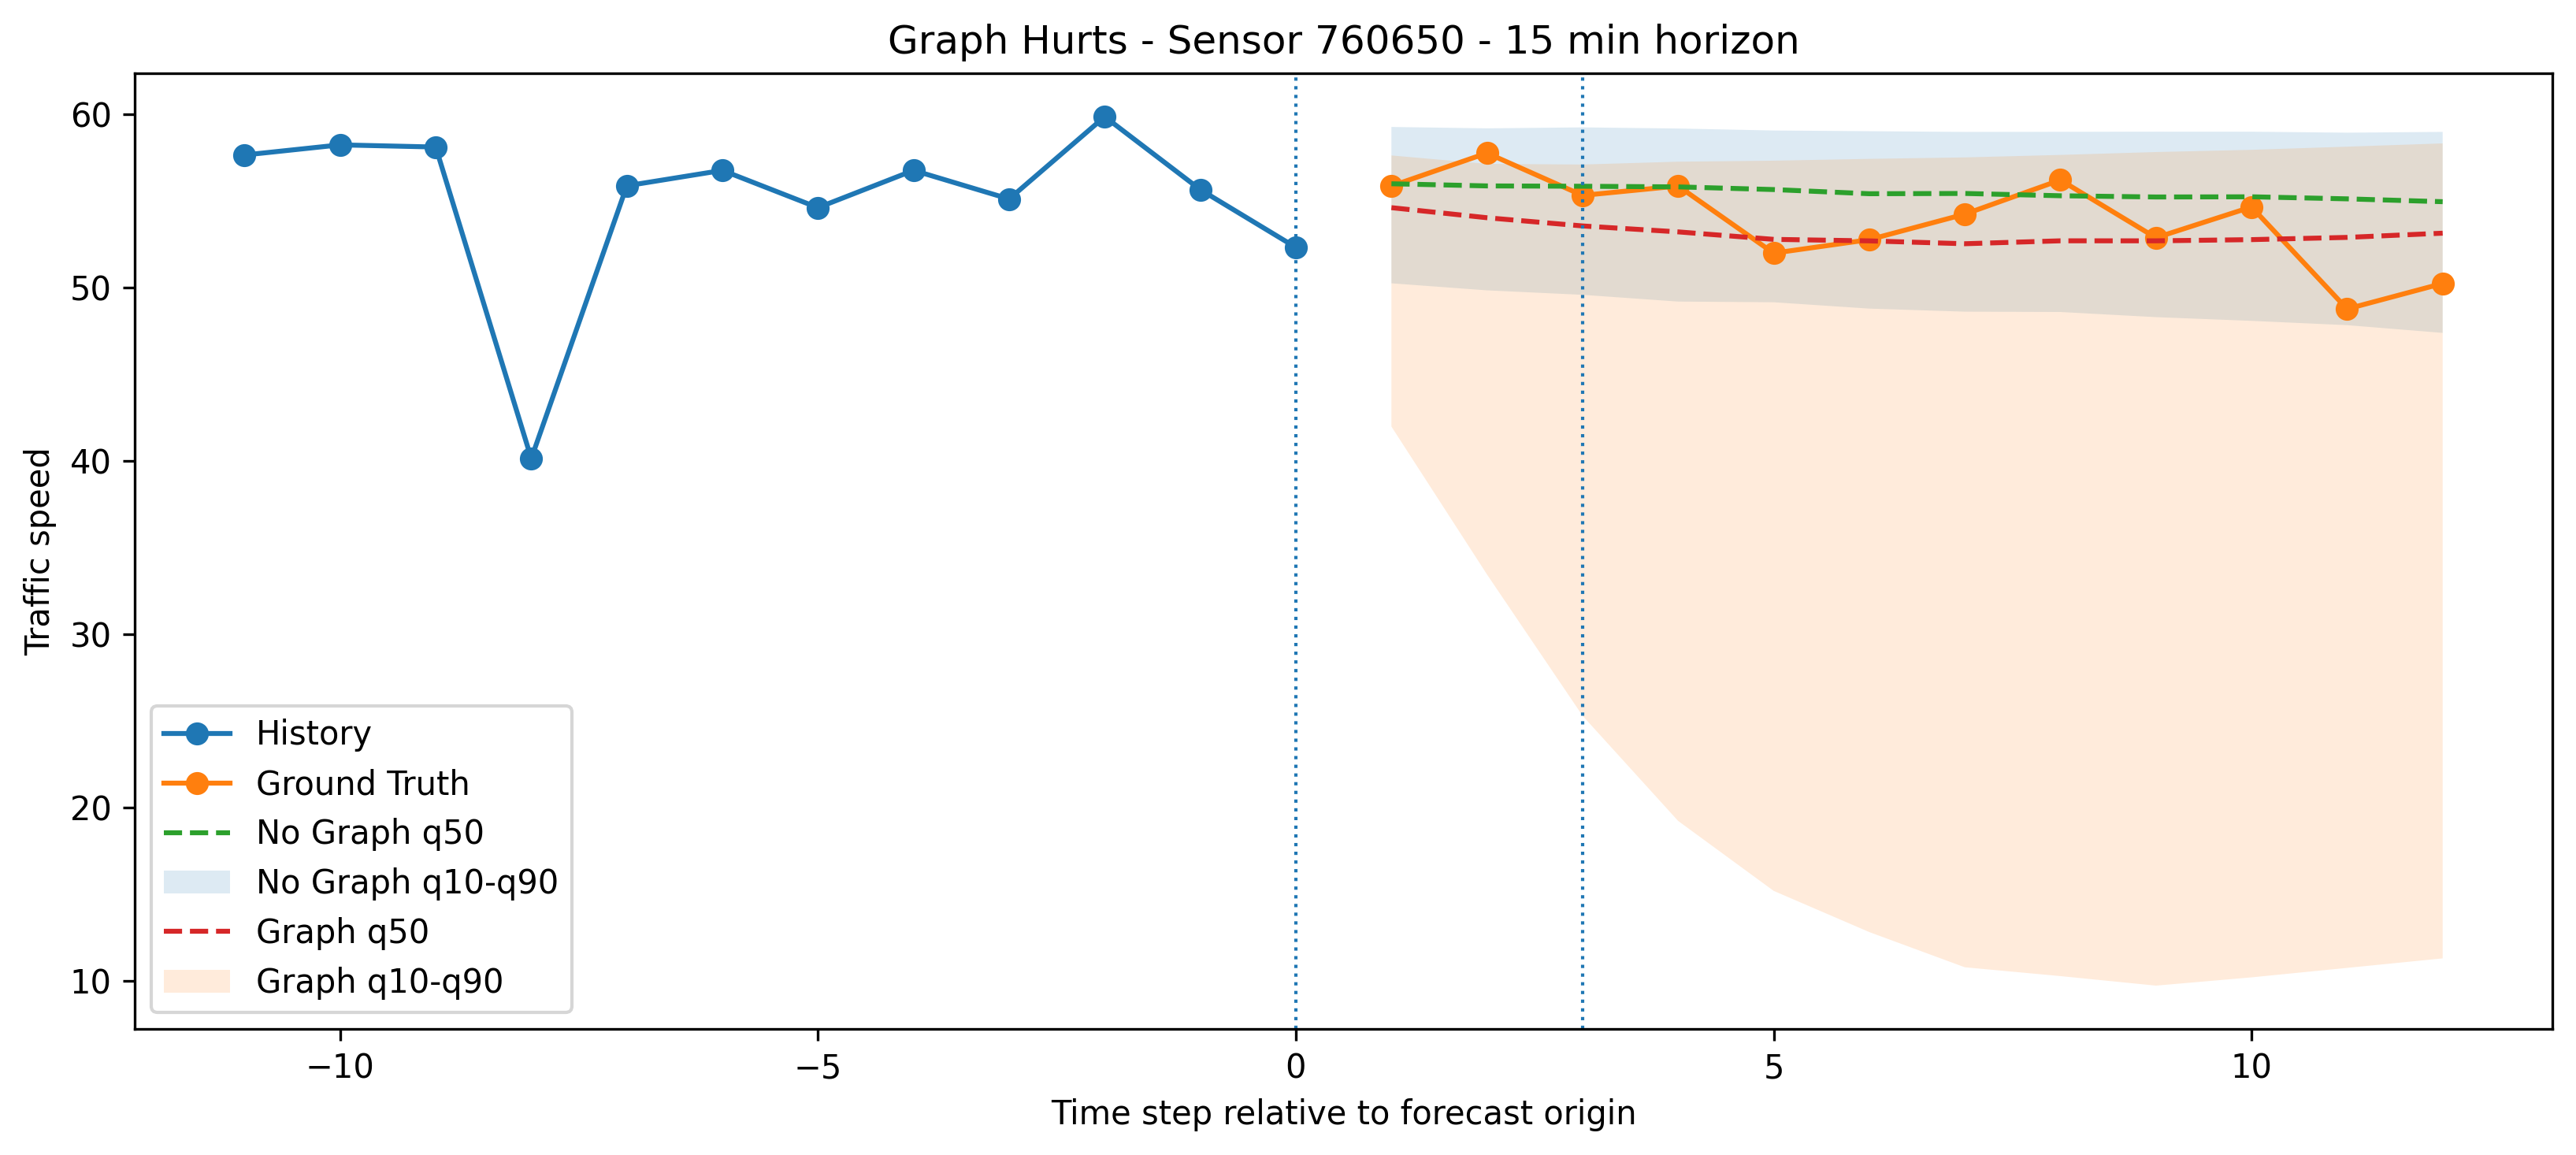
\includegraphics[width=\linewidth]{img/graph_impact_analysis/graph_hurts_h3_sensor_760650}
    \end{minipage}
    \hfill
    \begin{minipage}[b]{0.8\linewidth}
        \centering
        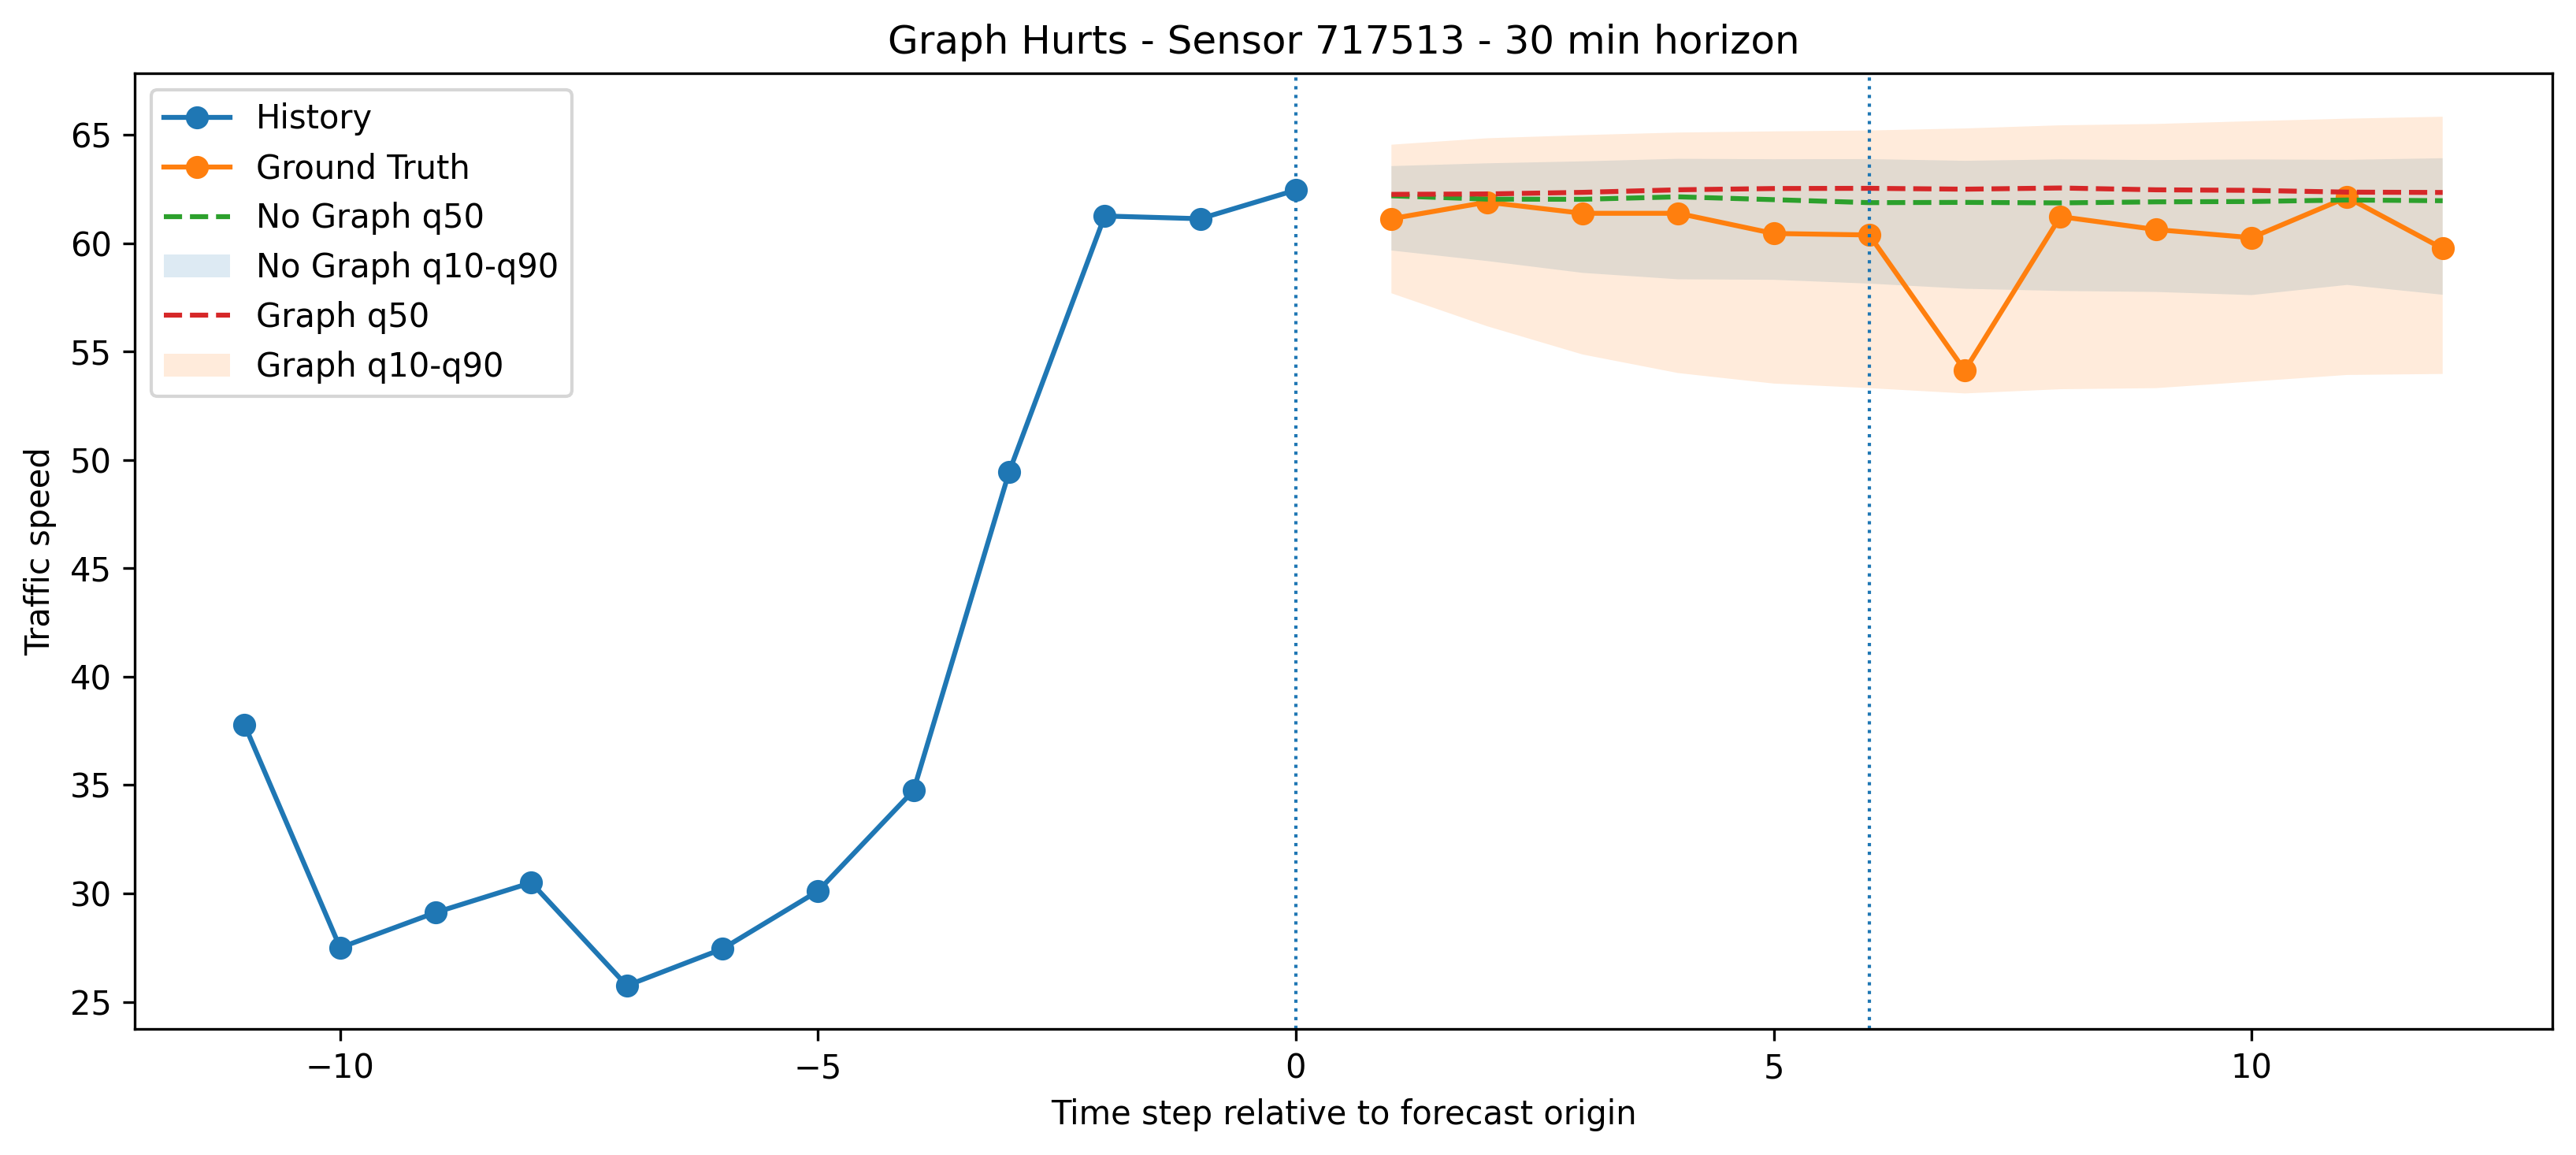
\includegraphics[width=\linewidth]{img/graph_impact_analysis/graph_hurts_h6_sensor_717513}
    \end{minipage}
    \hfill
    \begin{minipage}[b]{0.8\linewidth}
        \centering
        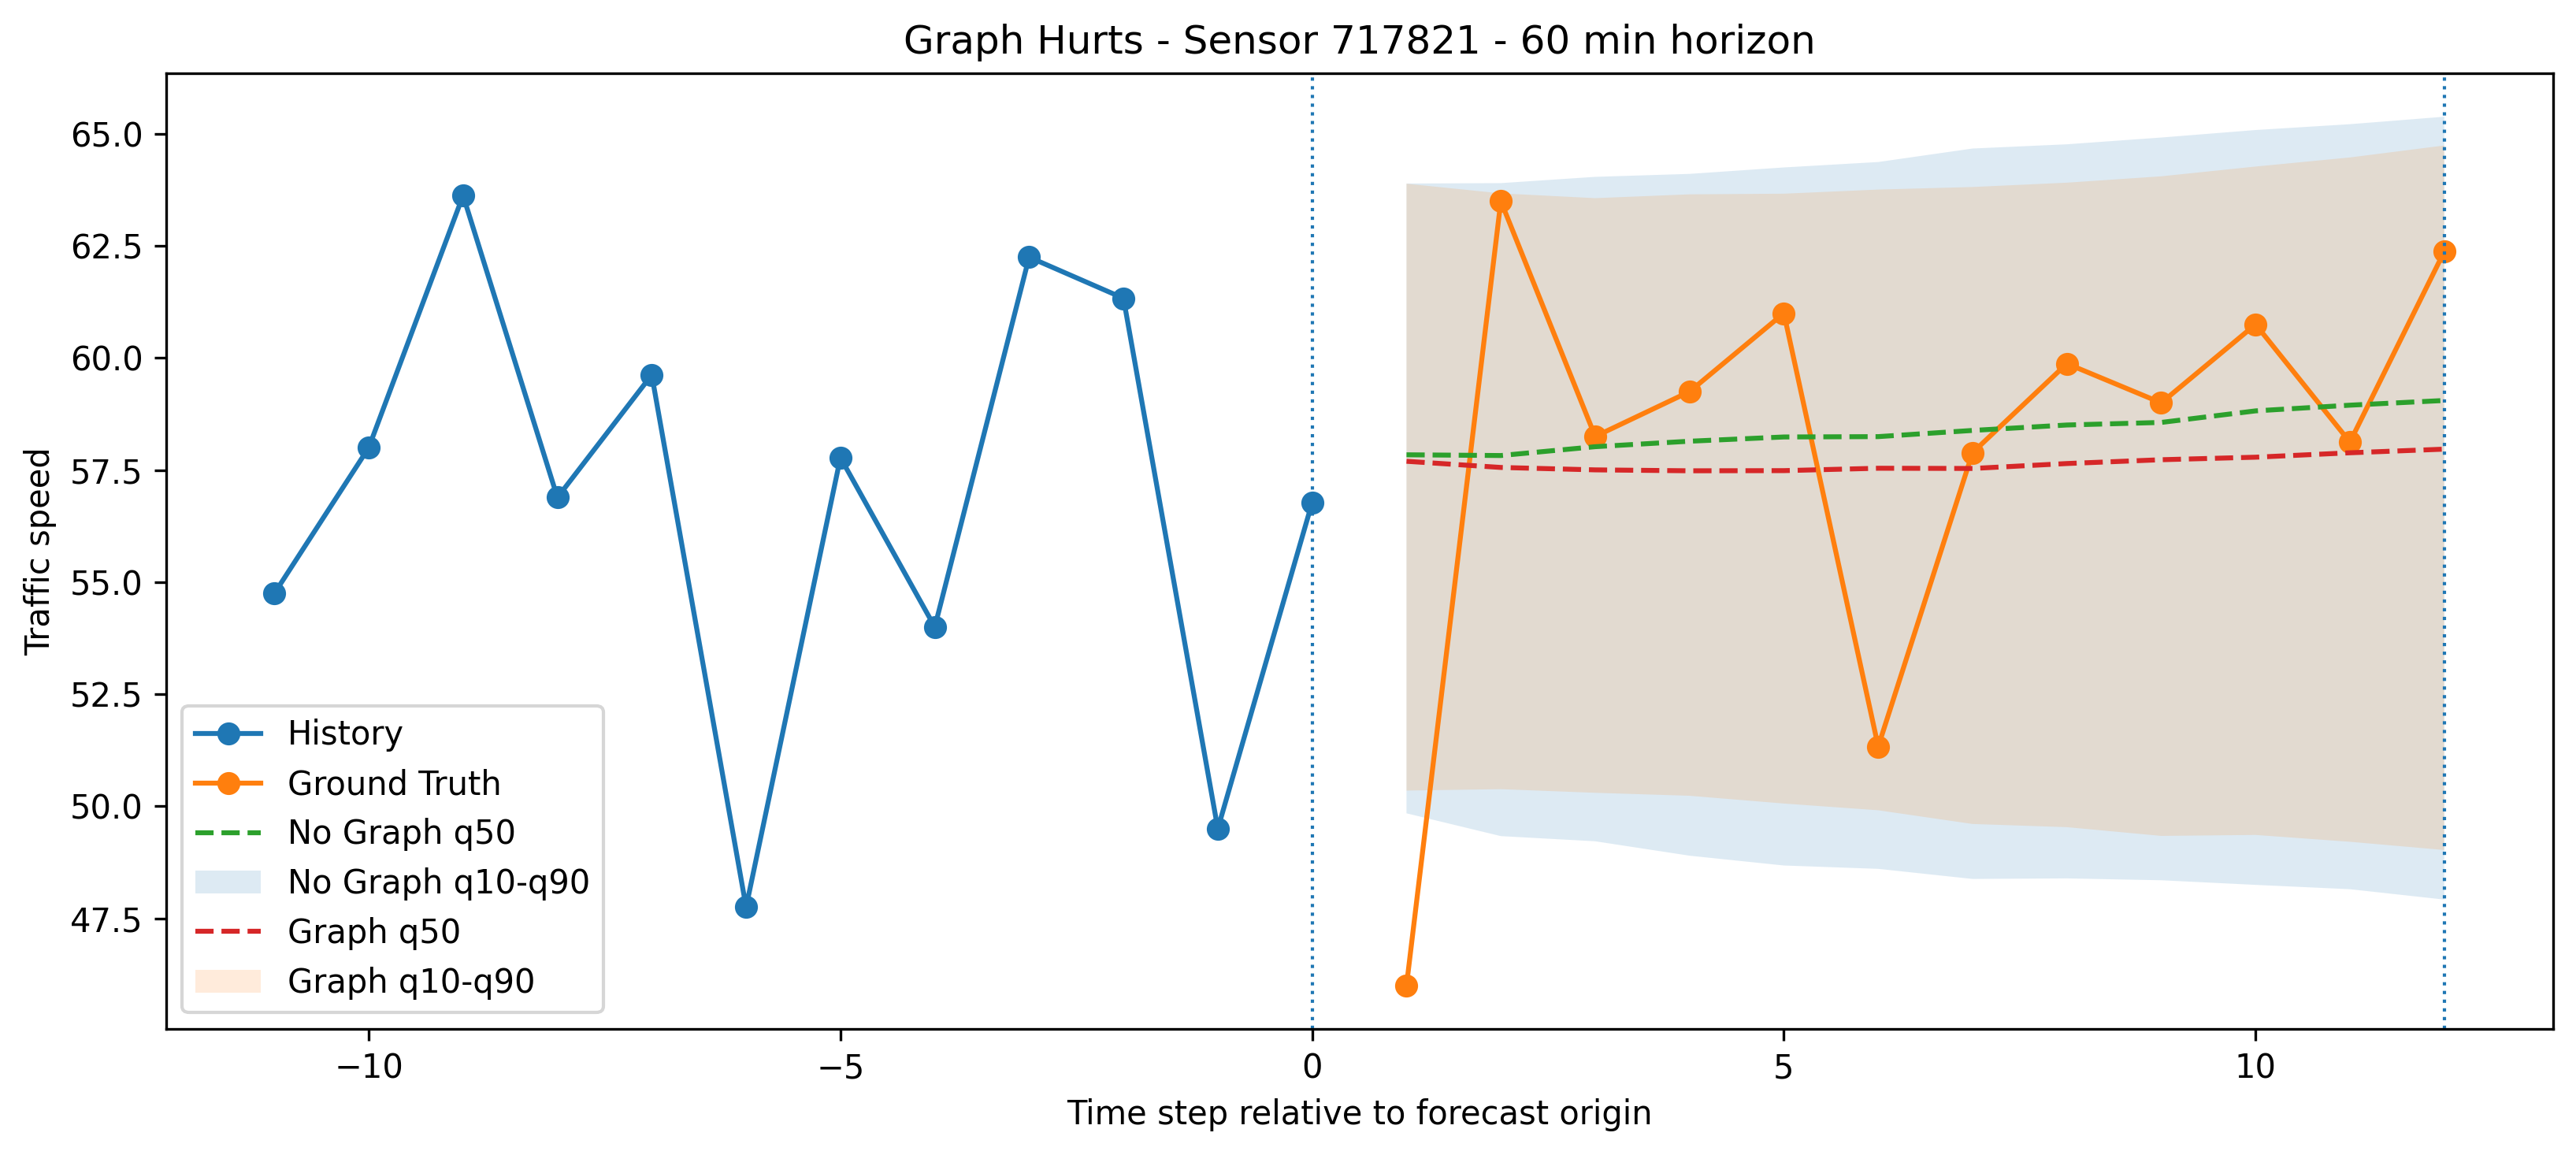
\includegraphics[width=\linewidth]{img/graph_impact_analysis/graph_hurts_h12_sensor_717821}
    \end{minipage}

    \caption{Representative forecasting examples in which the Graph-Temporal
model performs worse than the Temporal model at the 15-minute (top), 30-minute
(center), and 60-minute (bottom) forecasting horizons.}
    \label{fig:graph_hurt_examples}
\end{figure}


Figure~\ref{fig:graph_hurt_examples} instead reports representative cases in
which graph message passing increases the forecasting error. These examples
are particularly useful because they show that neighboring information is
not always informative for the future evolution of a given sensor. The
presence of such cases motivates a more detailed investigation of whether the
benefit of graph message passing can be related to the local graph structure.

\begin{figure}[t]
    \centering

    \begin{minipage}[b]{0.8\linewidth}
        \centering
        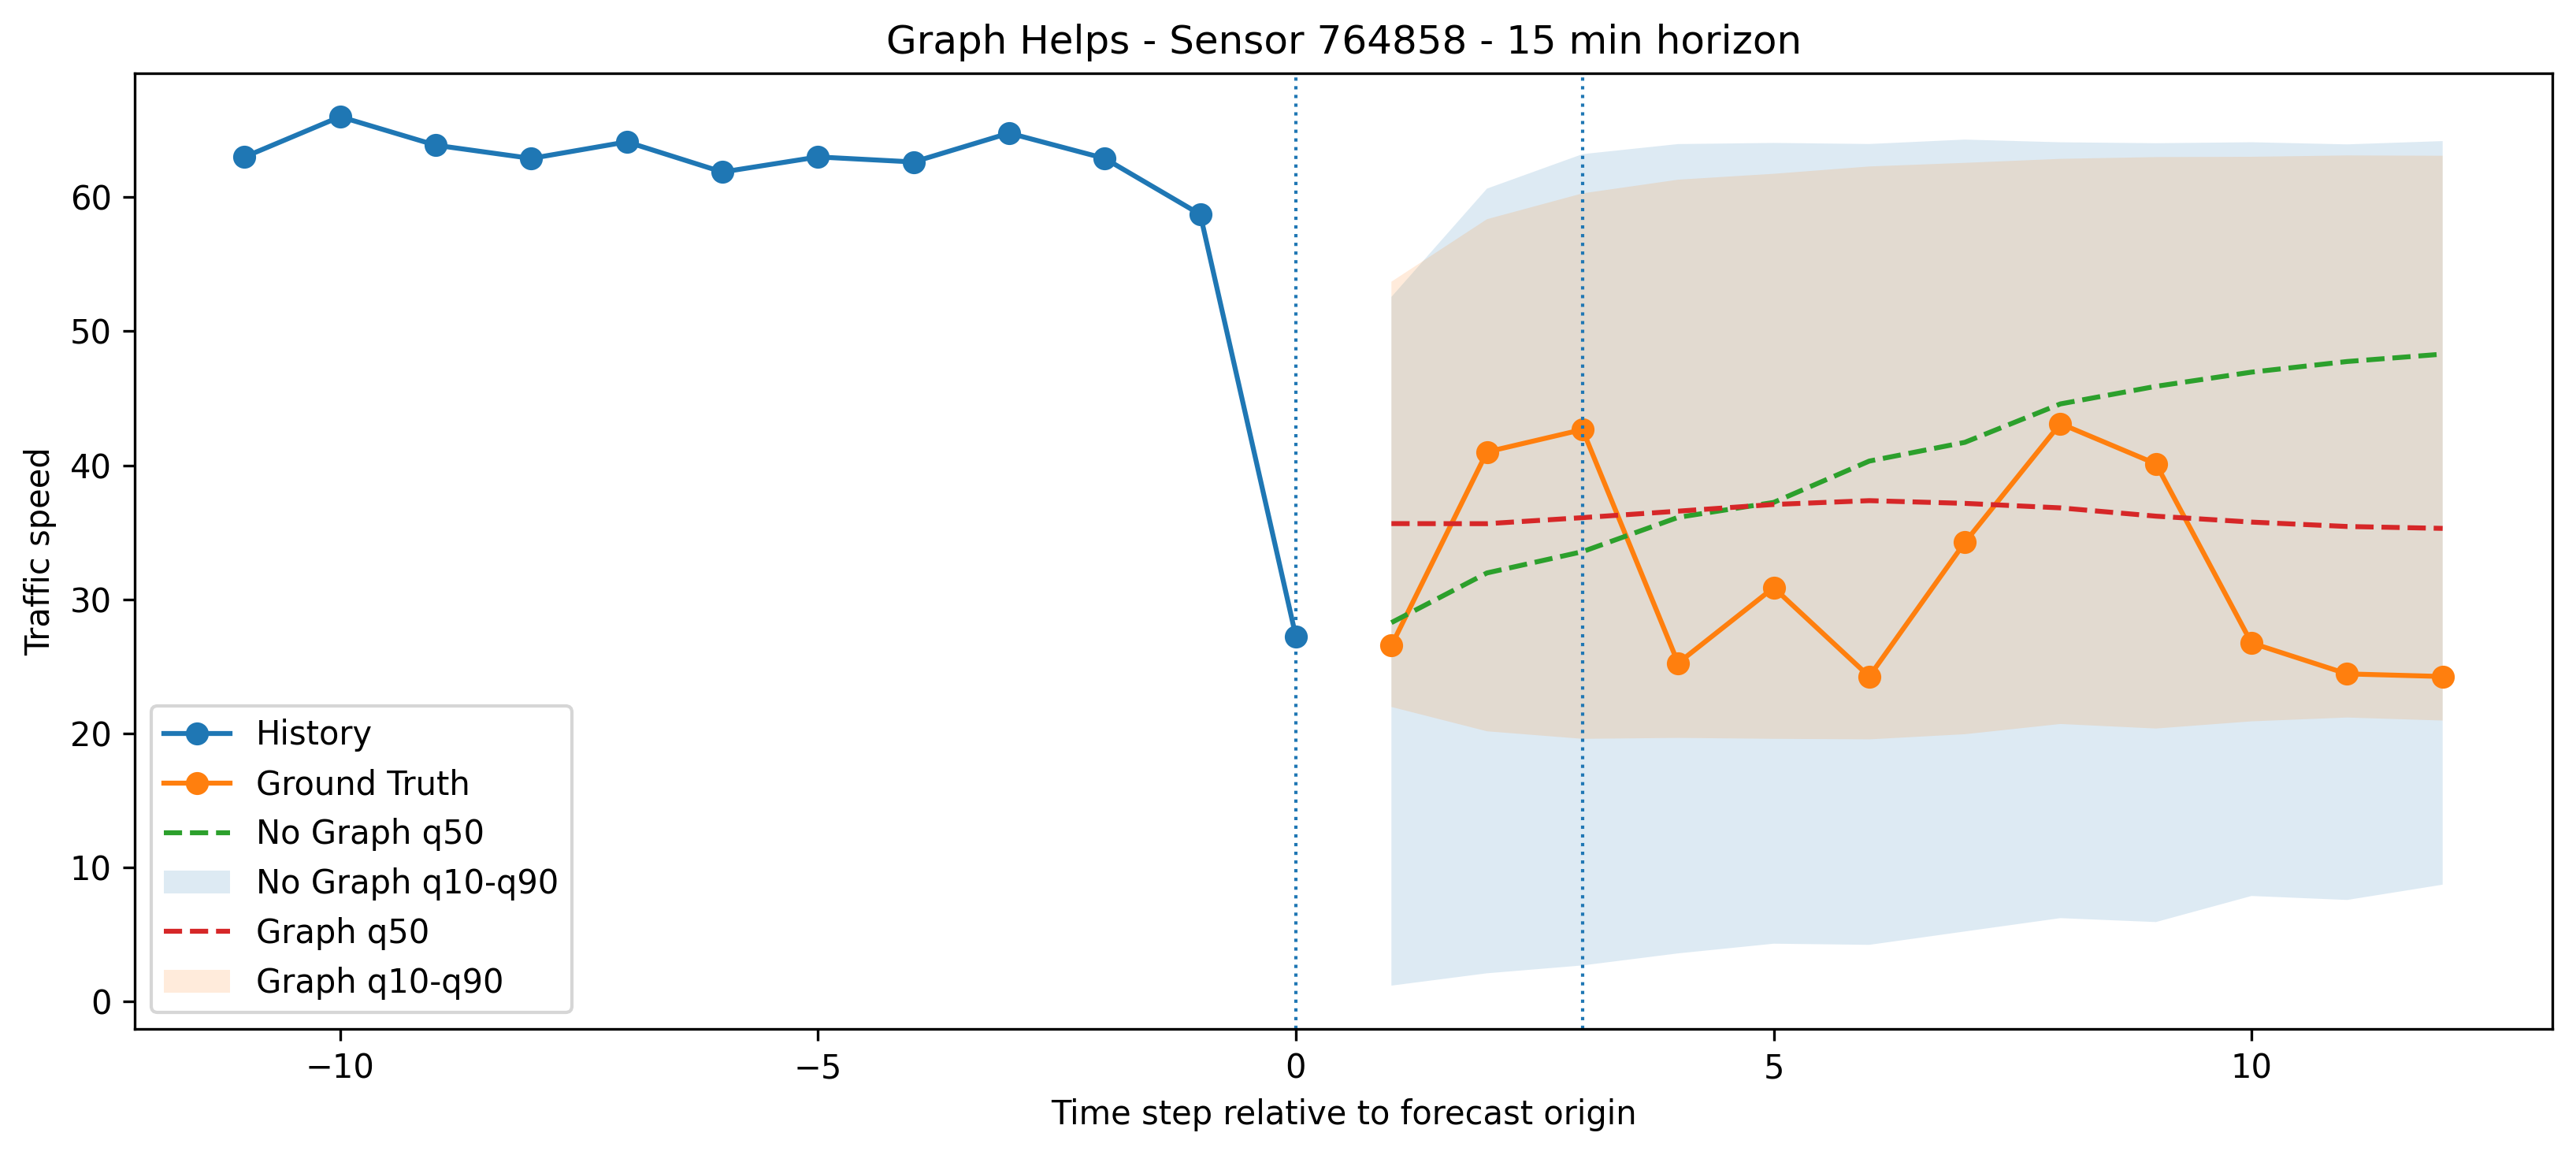
\includegraphics[width=\linewidth]{img/graph_impact_analysis/graph_helps_h3_sensor_764858}
    \end{minipage}
    \hfill
    \begin{minipage}[b]{0.8\linewidth}
        \centering
        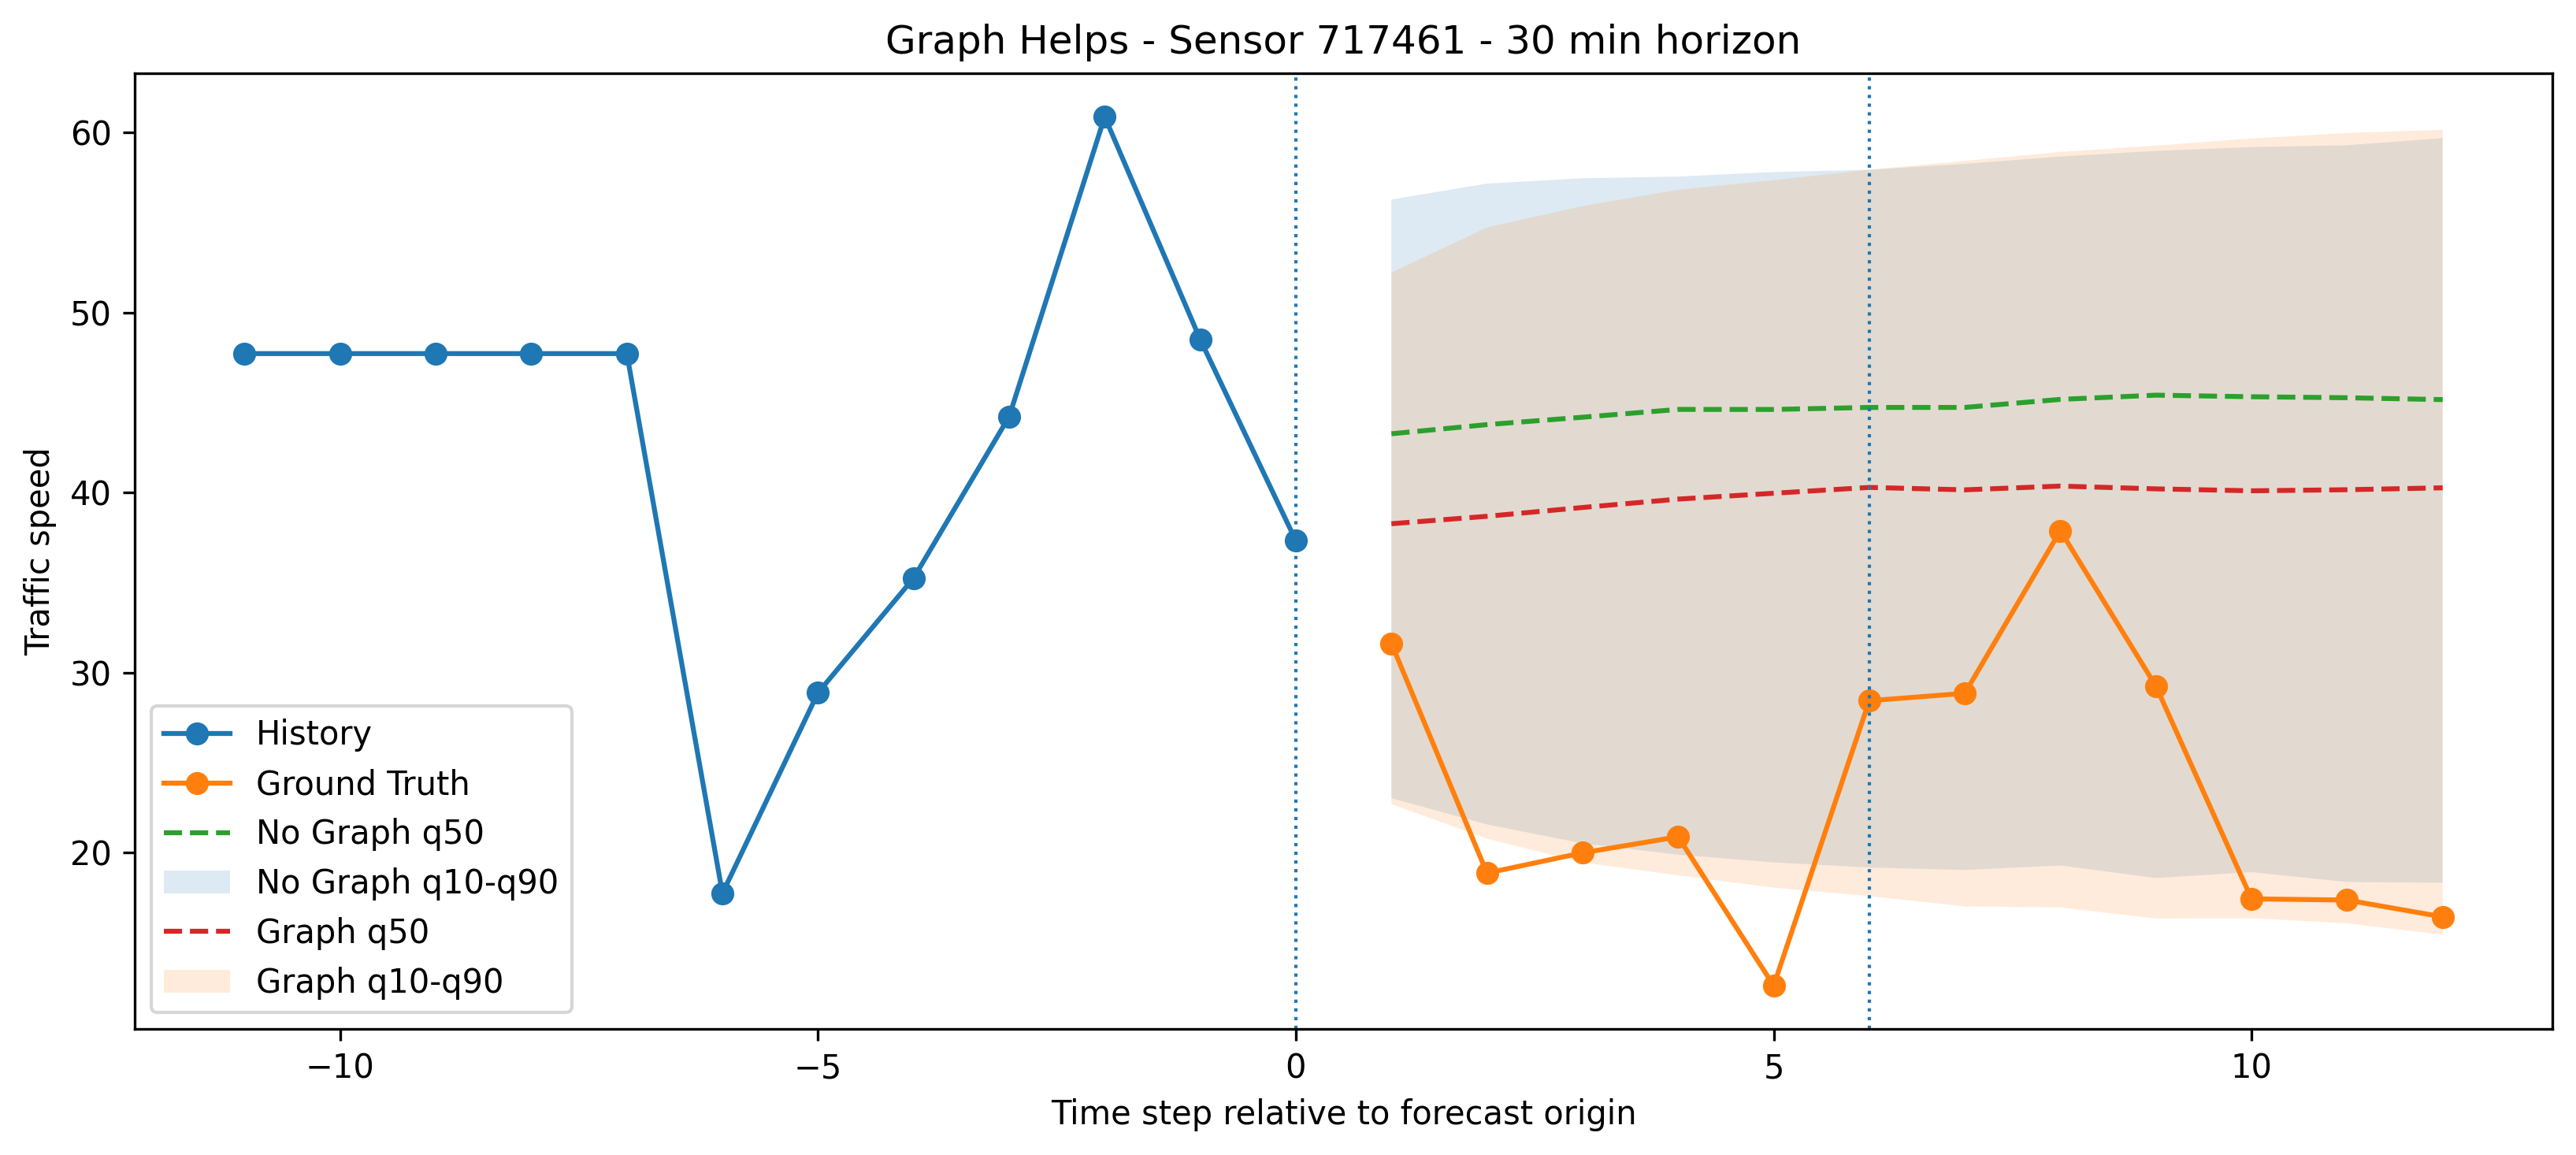
\includegraphics[width=\linewidth]{img/graph_impact_analysis/graph_helps_h6_sensor_717461}
    \end{minipage}
    \hfill
    \begin{minipage}[b]{0.8\linewidth}
        \centering
        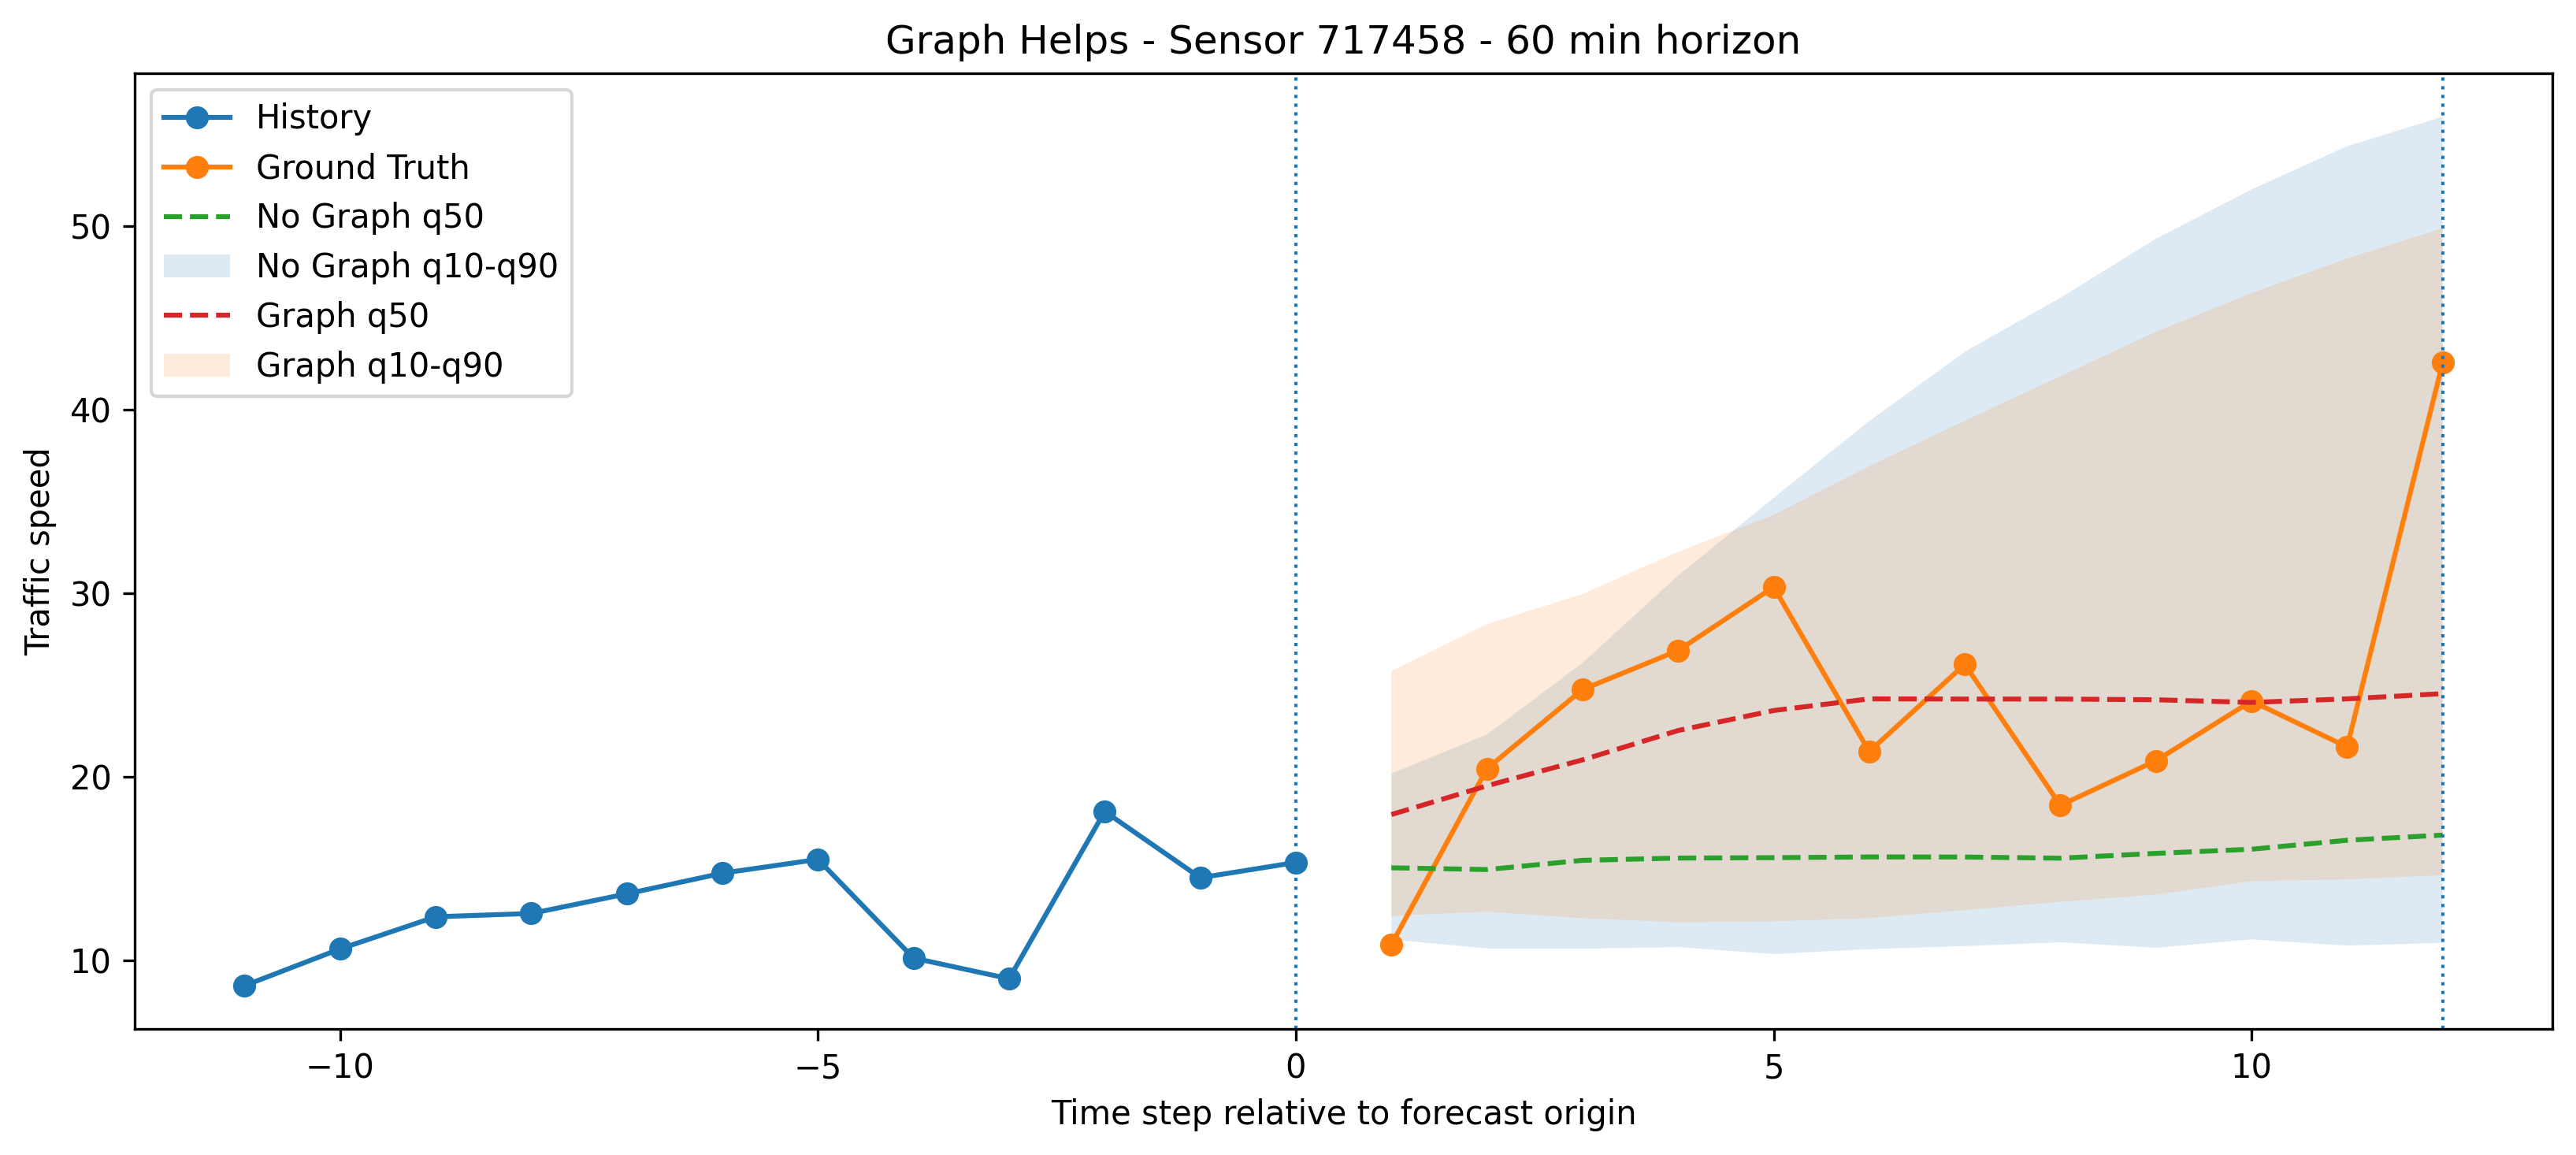
\includegraphics[width=\linewidth]{img/graph_impact_analysis/graph_helps_h12_sensor_717458}
    \end{minipage}

    \caption{Representative forecasting examples in which the Graph-Temporal
    model improves over the Temporal GRU at the 15-minute (top), 30-minute
    (center), and 60-minute (bottom) forecasting horizons.}
    \label{fig:graph_help_examples}
\end{figure}

Overall, these examples confirm that the effect of graph message passing is
sensor and time dependent. Although spatial information improves forecasting
accuracy for the large majority of sensors, it can occasionally introduce
information that does not improve the local prediction. This observation is
consistent with the small subset of sensors for which the Temporal GRU
achieves lower MAE.

\subsection{Effect of Diffusion Depth}
\label{subsec:diffusion_depth}

The main Graph-Temporal model uses a diffusion depth of $K=2$, allowing each
diffusion-style message-passing layer
 to combine information from the current node and from nodes
reached through one and two-step propagation. To investigate whether a
larger spatial receptive field provides additional benefits, a variant with
$K=3$ was trained while keeping the remaining model configuration unchanged.

Table~\ref{tab:diffusion_depth} compares the test performance of the two
configurations. Increasing the diffusion depth produces a small but consistent
reduction in MAE. However, the same behavior
is not observed for RMSE since $K=3$ model obtains slightly higher RMSE at all
three horizons. Therefore, the additional diffusion step
slightly improves the average absolute error but does not improve the model's
sensitivity to larger forecasting errors.


\begin{table}[t]
    \centering
    \caption{Test performance of the Graph-Temporal model with diffusion
    depths $K=2$ and $K=3$.}
    \label{tab:diffusion_depth}
    \resizebox{\linewidth}{!}{
    \begin{tabular}{ccrrrrrrrrrr}
        \toprule
        $K$ & Horizon &
        MAE & RMSE &
        Pinball$_{0.1}$ & Pinball$_{0.5}$ & Pinball$_{0.9}$ &
        Coverage (\%) & Interval Width & Crossing (\%) \\
        \midrule
        2 & 15 min & 2.901 & 5.511 & 0.845 & 1.451 & 0.597 & 78.44 & 8.929  & 0.031 \\
        2 & 30 min & 3.442 & 6.758 & 1.028 & 1.721 & 0.677 & 78.22 & 10.485 & 0.029 \\
        2 & 60 min & 4.244 & 8.378 & 1.320 & 2.122 & 0.775 & 78.13 & 12.470 & 0.048 \\
        \midrule
        3 & 15 min & 2.888 & 5.533 & 0.846 & 1.444 & 0.593 & 78.84 & 8.723  & 0.028 \\
        3 & 30 min & 3.424 & 6.799 & 1.030 & 1.712 & 0.673 & 77.87 & 9.948  & 0.034 \\
        3 & 60 min & 4.203 & 8.384 & 1.322 & 2.102 & 0.770 & 77.50 & 11.781 & 0.055 \\
        \bottomrule
    \end{tabular}}
\end{table}


\begin{figure}[t]
    \centering

    % First row: point forecasting metrics
    \begin{minipage}[b]{0.48\linewidth}
        \centering
        
\includegraphics[width=\linewidth]{img/graph_temporal/variant_comparison/mae_graph_temporal_variant_comparison}
    \end{minipage}
    \hfill
    \begin{minipage}[b]{0.48\linewidth}
        \centering
        
\includegraphics[width=\linewidth]{img/graph_temporal/variant_comparison/rmse_graph_temporal_variant_comparison}
    \end{minipage}

    \vspace{0.4cm}

    % Second row: probabilistic metrics
    \begin{minipage}[b]{0.48\linewidth}
        \centering
        
\includegraphics[width=\linewidth]{img/graph_temporal/variant_comparison//coverage_graph_temporal_variant_comparison}
    \end{minipage}
    \hfill
    \begin{minipage}[b]{0.48\linewidth}
        \centering
        
\includegraphics[width=\linewidth]{img/graph_temporal/variant_comparison/interval_width_graph_temporal_variant_comparison}
    \end{minipage}

    \caption{Comparison of the Graph-Temporal model with diffusion depths
    $K=2$ and $K=3$. The top row reports point forecasting performance in
    terms of MAE (left) and RMSE (right), while the bottom row reports
    empirical coverage (left) and prediction interval width (right) across
    the three forecasting horizons.}
    \label{fig:diffusion_depth_comparison}
\end{figure}

The comparison is also illustrated in
Figure~\ref{fig:diffusion_depth_comparison}. The effect of the additional
diffusion step is particularly visible in the probabilistic forecasts.
The $K=3$ model produces narrower prediction intervals at every horizon.
At the shortest horizon, this increased sharpness is accompanied by a small
improvement in coverage. At the longer forecasting horizons, however, the
sharper intervals obtained with $K=3$ come at the cost of increased
undercoverage. Quantile crossing remains negligible for both configurations.

The Pinball Loss values show a similarly limited effect of increasing the
diffusion depth. The $K=3$ configuration slightly improves the median and
upper-quantile losses at all horizons, while the loss associated with the
lower quantile slightly increases. Overall, increasing the diffusion depth
does not produce a consistent improvement across all probabilistic metrics.

The two configurations also exhibit different computational behavior. The
$K=2$ model was trained for 106 epochs, whereas the $K=3$ variant stopped
after 85 epochs. Despite requiring fewer epochs, the additional diffusion
step increases the computational cost of each epoch: the average training
time rises from approximately 19.3 seconds per epoch for $K=2$ to 22.0
seconds for $K=3$, an increase of about 14\%. The total training times are
approximately 34.0 and 31.1 minutes, respectively, with the lower total
training time of $K=3$ resulting from earlier stopping rather than lower
per-epoch computational complexity.

Overall, increasing the diffusion depth from $K=2$ to $K=3$ provides only
modest improvements in MAE and median Pinball Loss, while slightly increasing
RMSE and reducing coverage at the longer horizons. It also increases the
computational cost of each training epoch. For these reasons, $K=2$ was
retained for the main Graph-Temporal model, providing a more balanced
trade-off between forecasting accuracy, probabilistic reliability, and
computational complexity.

\subsection{Graph Ablation: Weighted vs. Binary Adjacency}
\label{subsec:weighted_binary}

The previous experiments use the original weighted adjacency matrix provided
with METR-LA. To investigate whether the edge weights contribute to the
forecasting performance or whether the graph connectivity alone is sufficient,
an ablation experiment was performed by replacing every non-zero edge weight
with one. The resulting binary adjacency matrix preserves the original graph
topology but removes information about the relative strength of the
connections. As for the weighted graph, the binary adjacency matrix was
row-normalized before being used for diffusion message passing.

Table~\ref{tab:weighted_binary} compares the two graph representations on the
test set. The weighted graph consistently achieves slightly lower point forecasting
errors and the difference becomes larger as the forecasting horizon increases.


\begin{table}[t]
    \centering
    \caption{Test performance of the Graph-Temporal model using the weighted
    and binary adjacency matrices.}
    \label{tab:weighted_binary}
    \resizebox{\linewidth}{!}{
    \begin{tabular}{llrrrrrrrr}
        \toprule
        Graph & Horizon &
        MAE & RMSE &
        Pinball$_{0.1}$ & Pinball$_{0.5}$ & Pinball$_{0.9}$ &
        Coverage (\%) & Interval Width \\
        \midrule
        Weighted
        & 15 min & 2.901 & 5.511 & 0.845 & 1.451 & 0.597 & 78.44 & 8.929 \\
        & 30 min & 3.442 & 6.758 & 1.028 & 1.721 & 0.677 & 78.22 & 10.485 \\
        & 60 min & 4.244 & 8.378 & 1.320 & 2.122 & 0.775 & 78.13 & 12.470 \\
        \midrule
        Binary
        & 15 min & 2.948 & 5.682 & 0.873 & 1.474 & 0.610 & 79.54 & 8.878 \\
        & 30 min & 3.543 & 7.033 & 1.084 & 1.772 & 0.699 & 78.80 & 10.424 \\
        & 60 min & 4.443 & 8.754 & 1.417 & 2.222 & 0.807 & 78.11 & 12.593 \\
        \bottomrule
    \end{tabular}}
\end{table}


\begin{figure}[t]
    \centering

    % First row: point forecasting metrics
    \begin{minipage}[b]{0.48\linewidth}
        \centering
        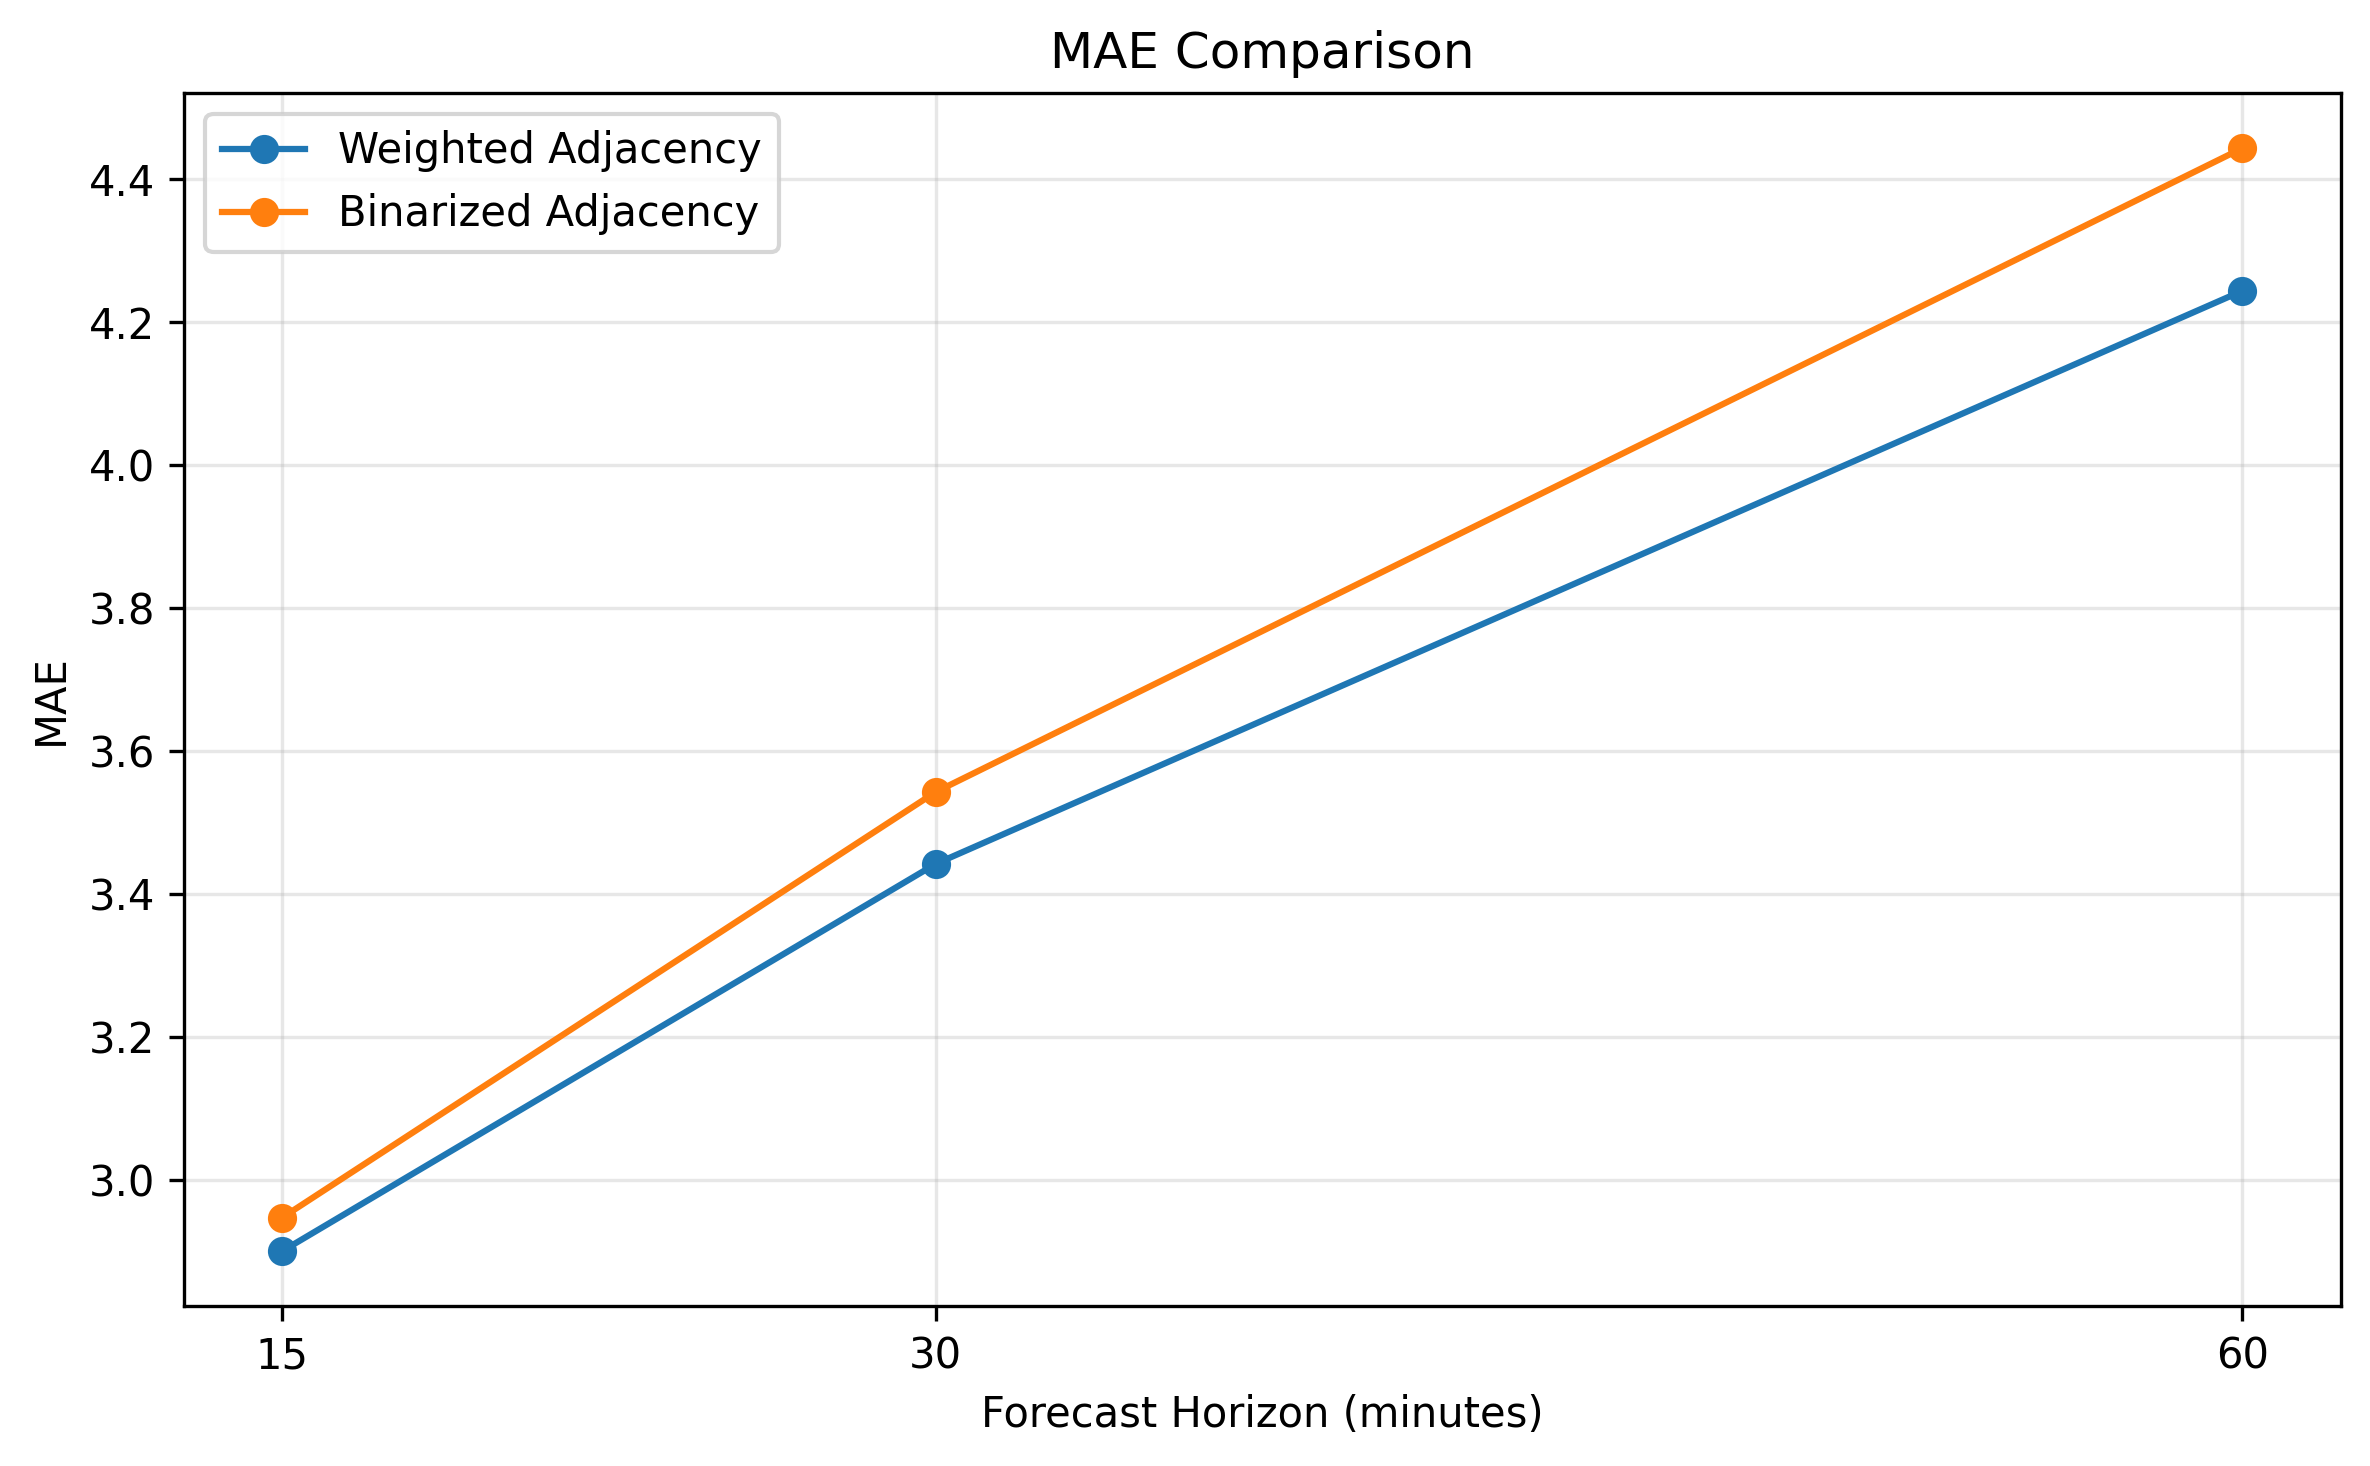
\includegraphics[width=\linewidth]{img/graph_temporal/ablation_comparison/mae_graph_temporal_variant_comparison}
    \end{minipage}
    \hfill
    \begin{minipage}[b]{0.48\linewidth}
        \centering
        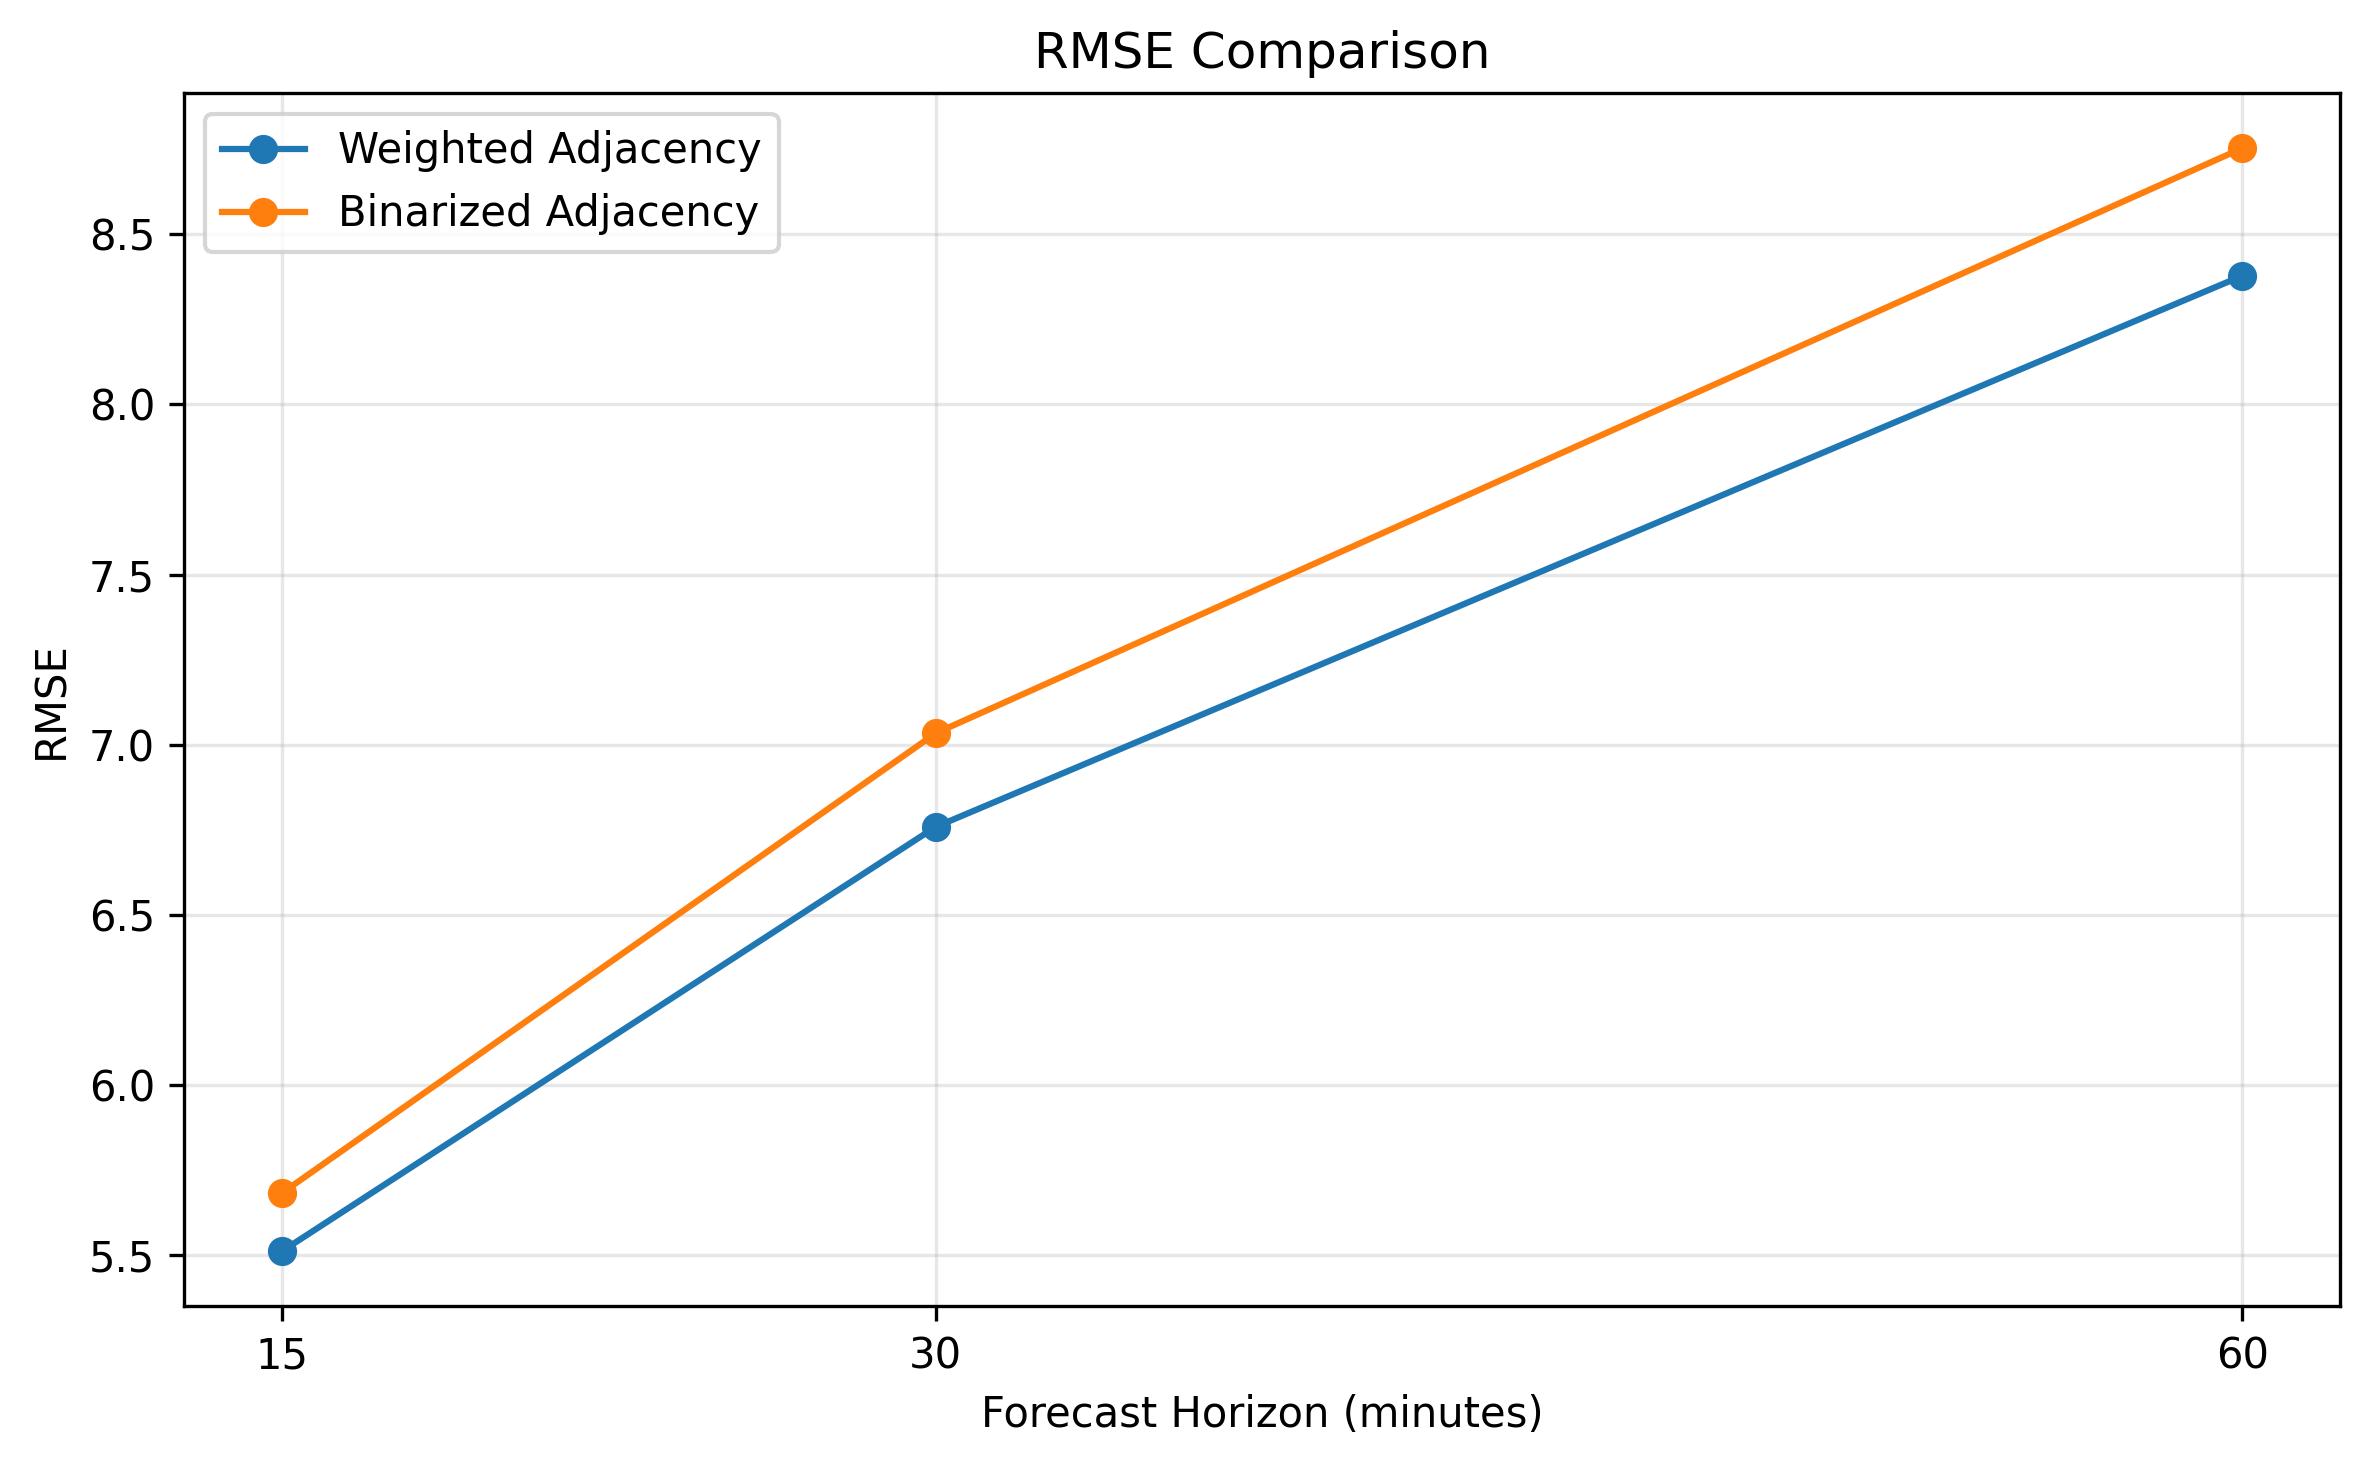
\includegraphics[width=\linewidth]{img/graph_temporal/ablation_comparison/rmse_graph_temporal_variant_comparison}
    \end{minipage}

    \vspace{0.4cm}

    % Second row: probabilistic metrics
    \begin{minipage}[b]{0.48\linewidth}
        \centering
        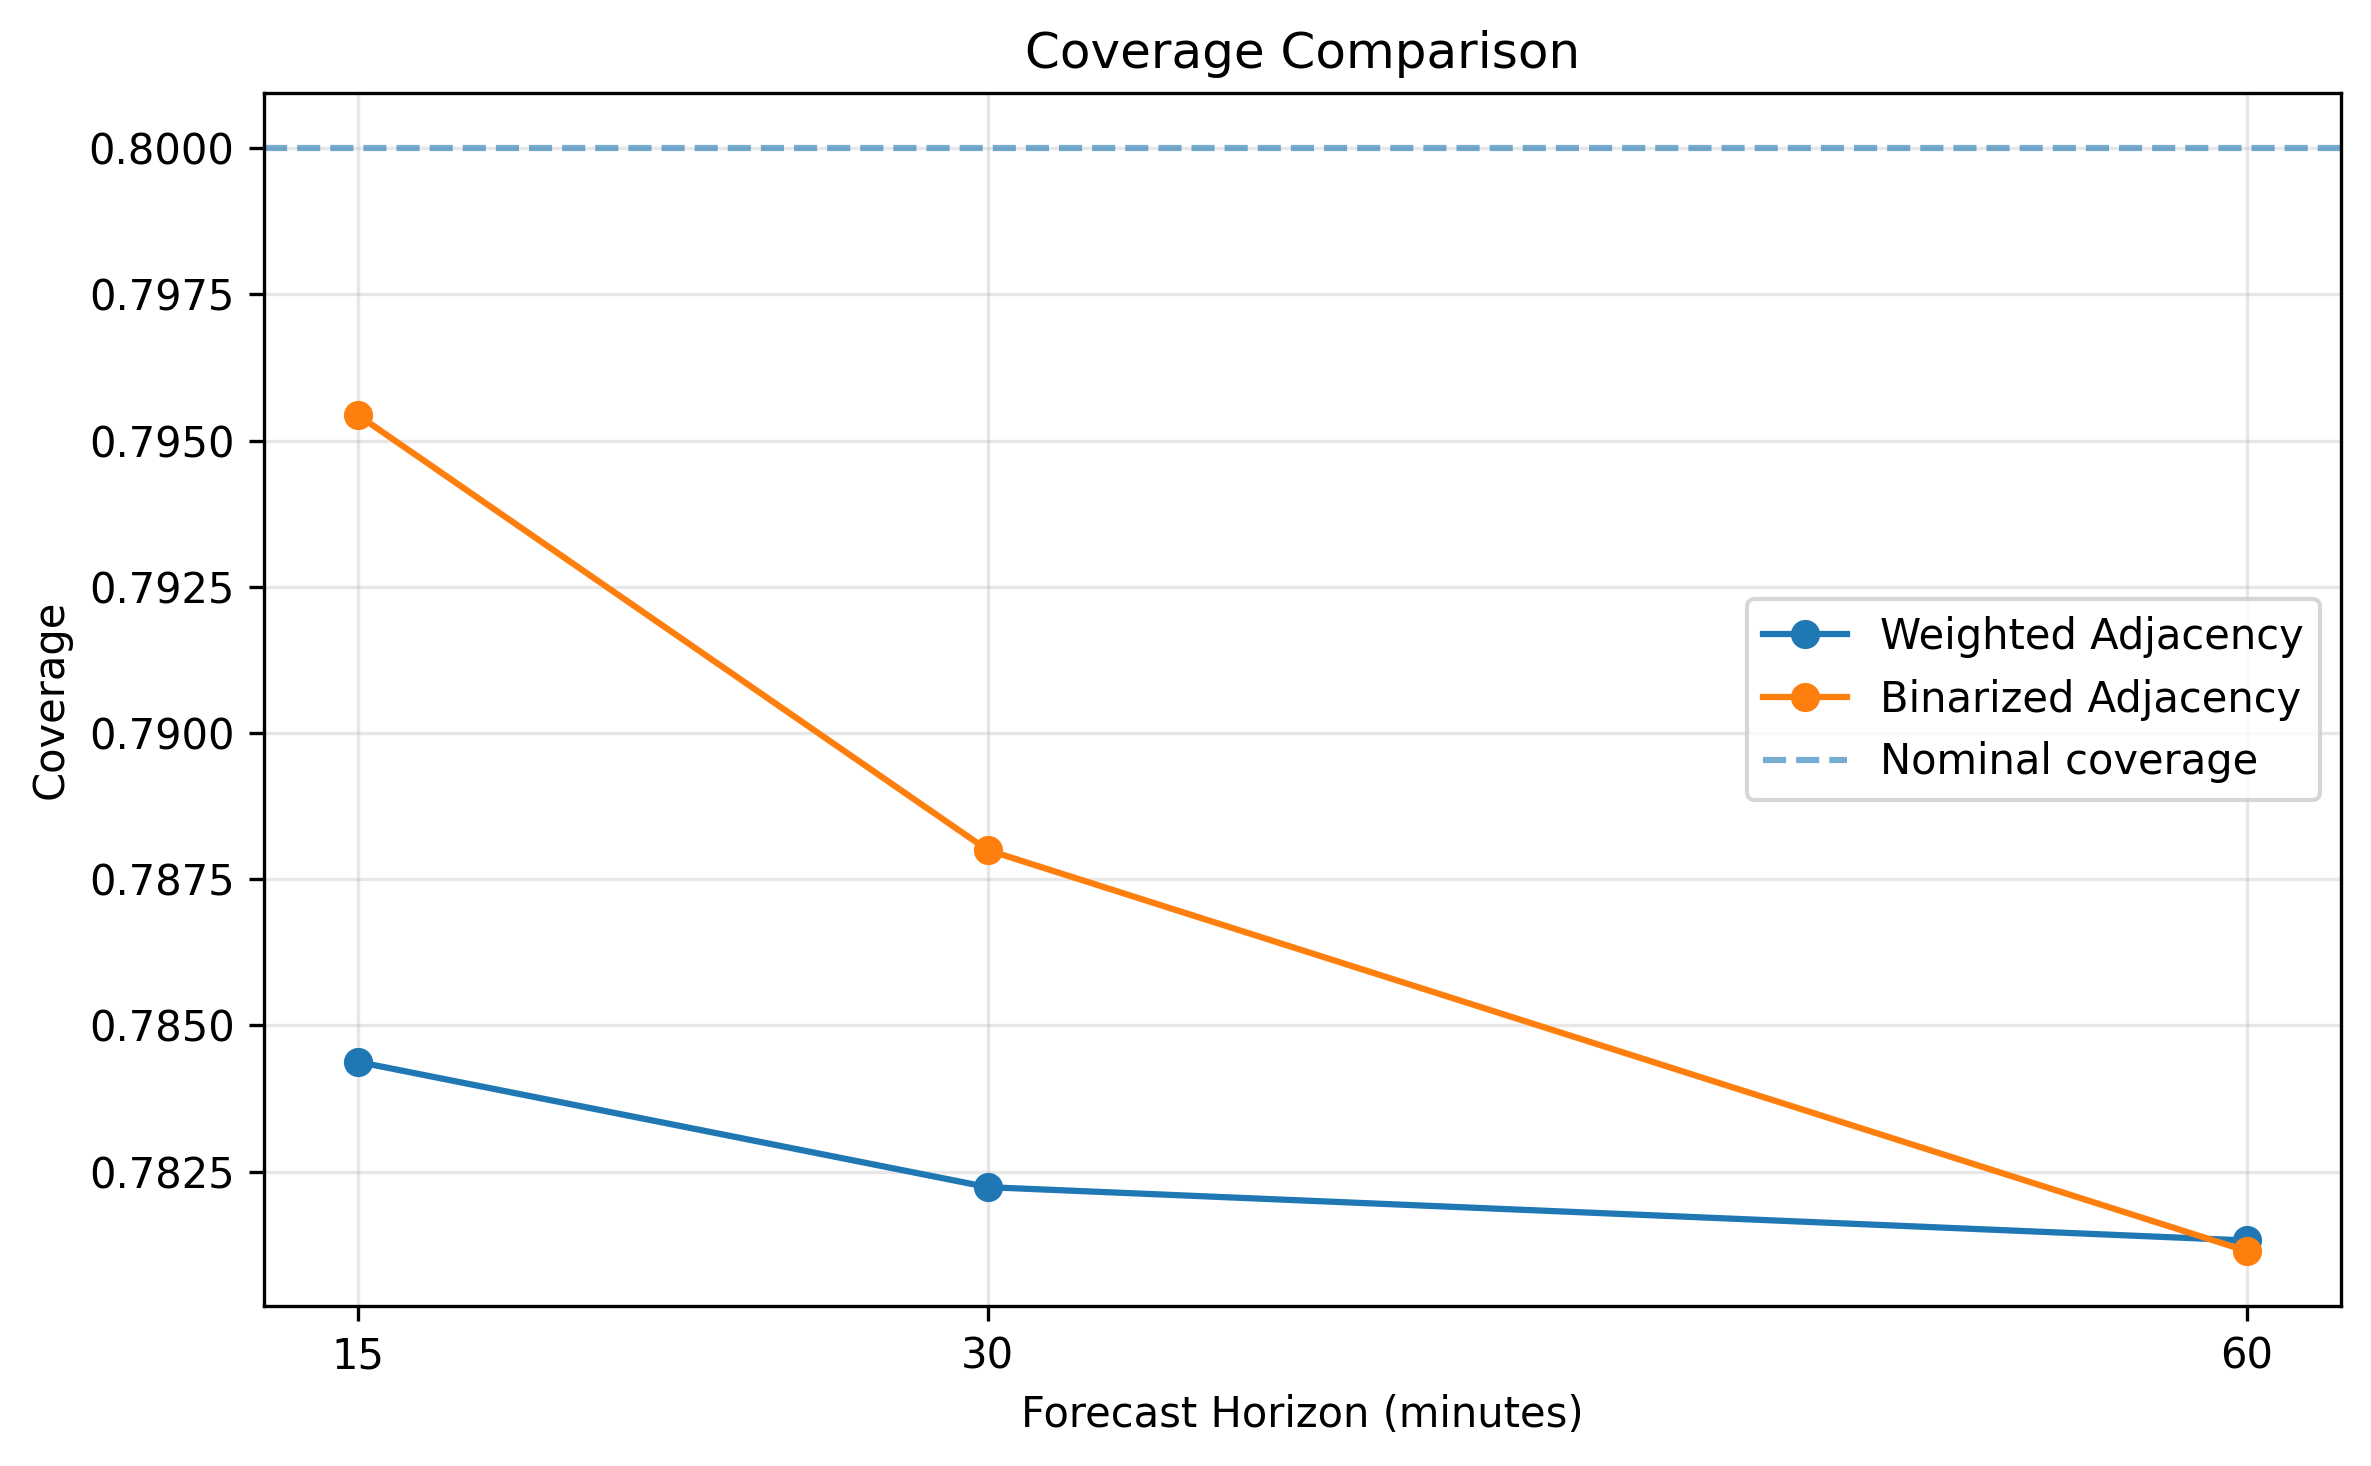
\includegraphics[width=\linewidth]{img/graph_temporal/ablation_comparison/coverage_graph_temporal_variant_comparison}
    \end{minipage}
    \hfill
    \begin{minipage}[b]{0.48\linewidth}
        \centering
        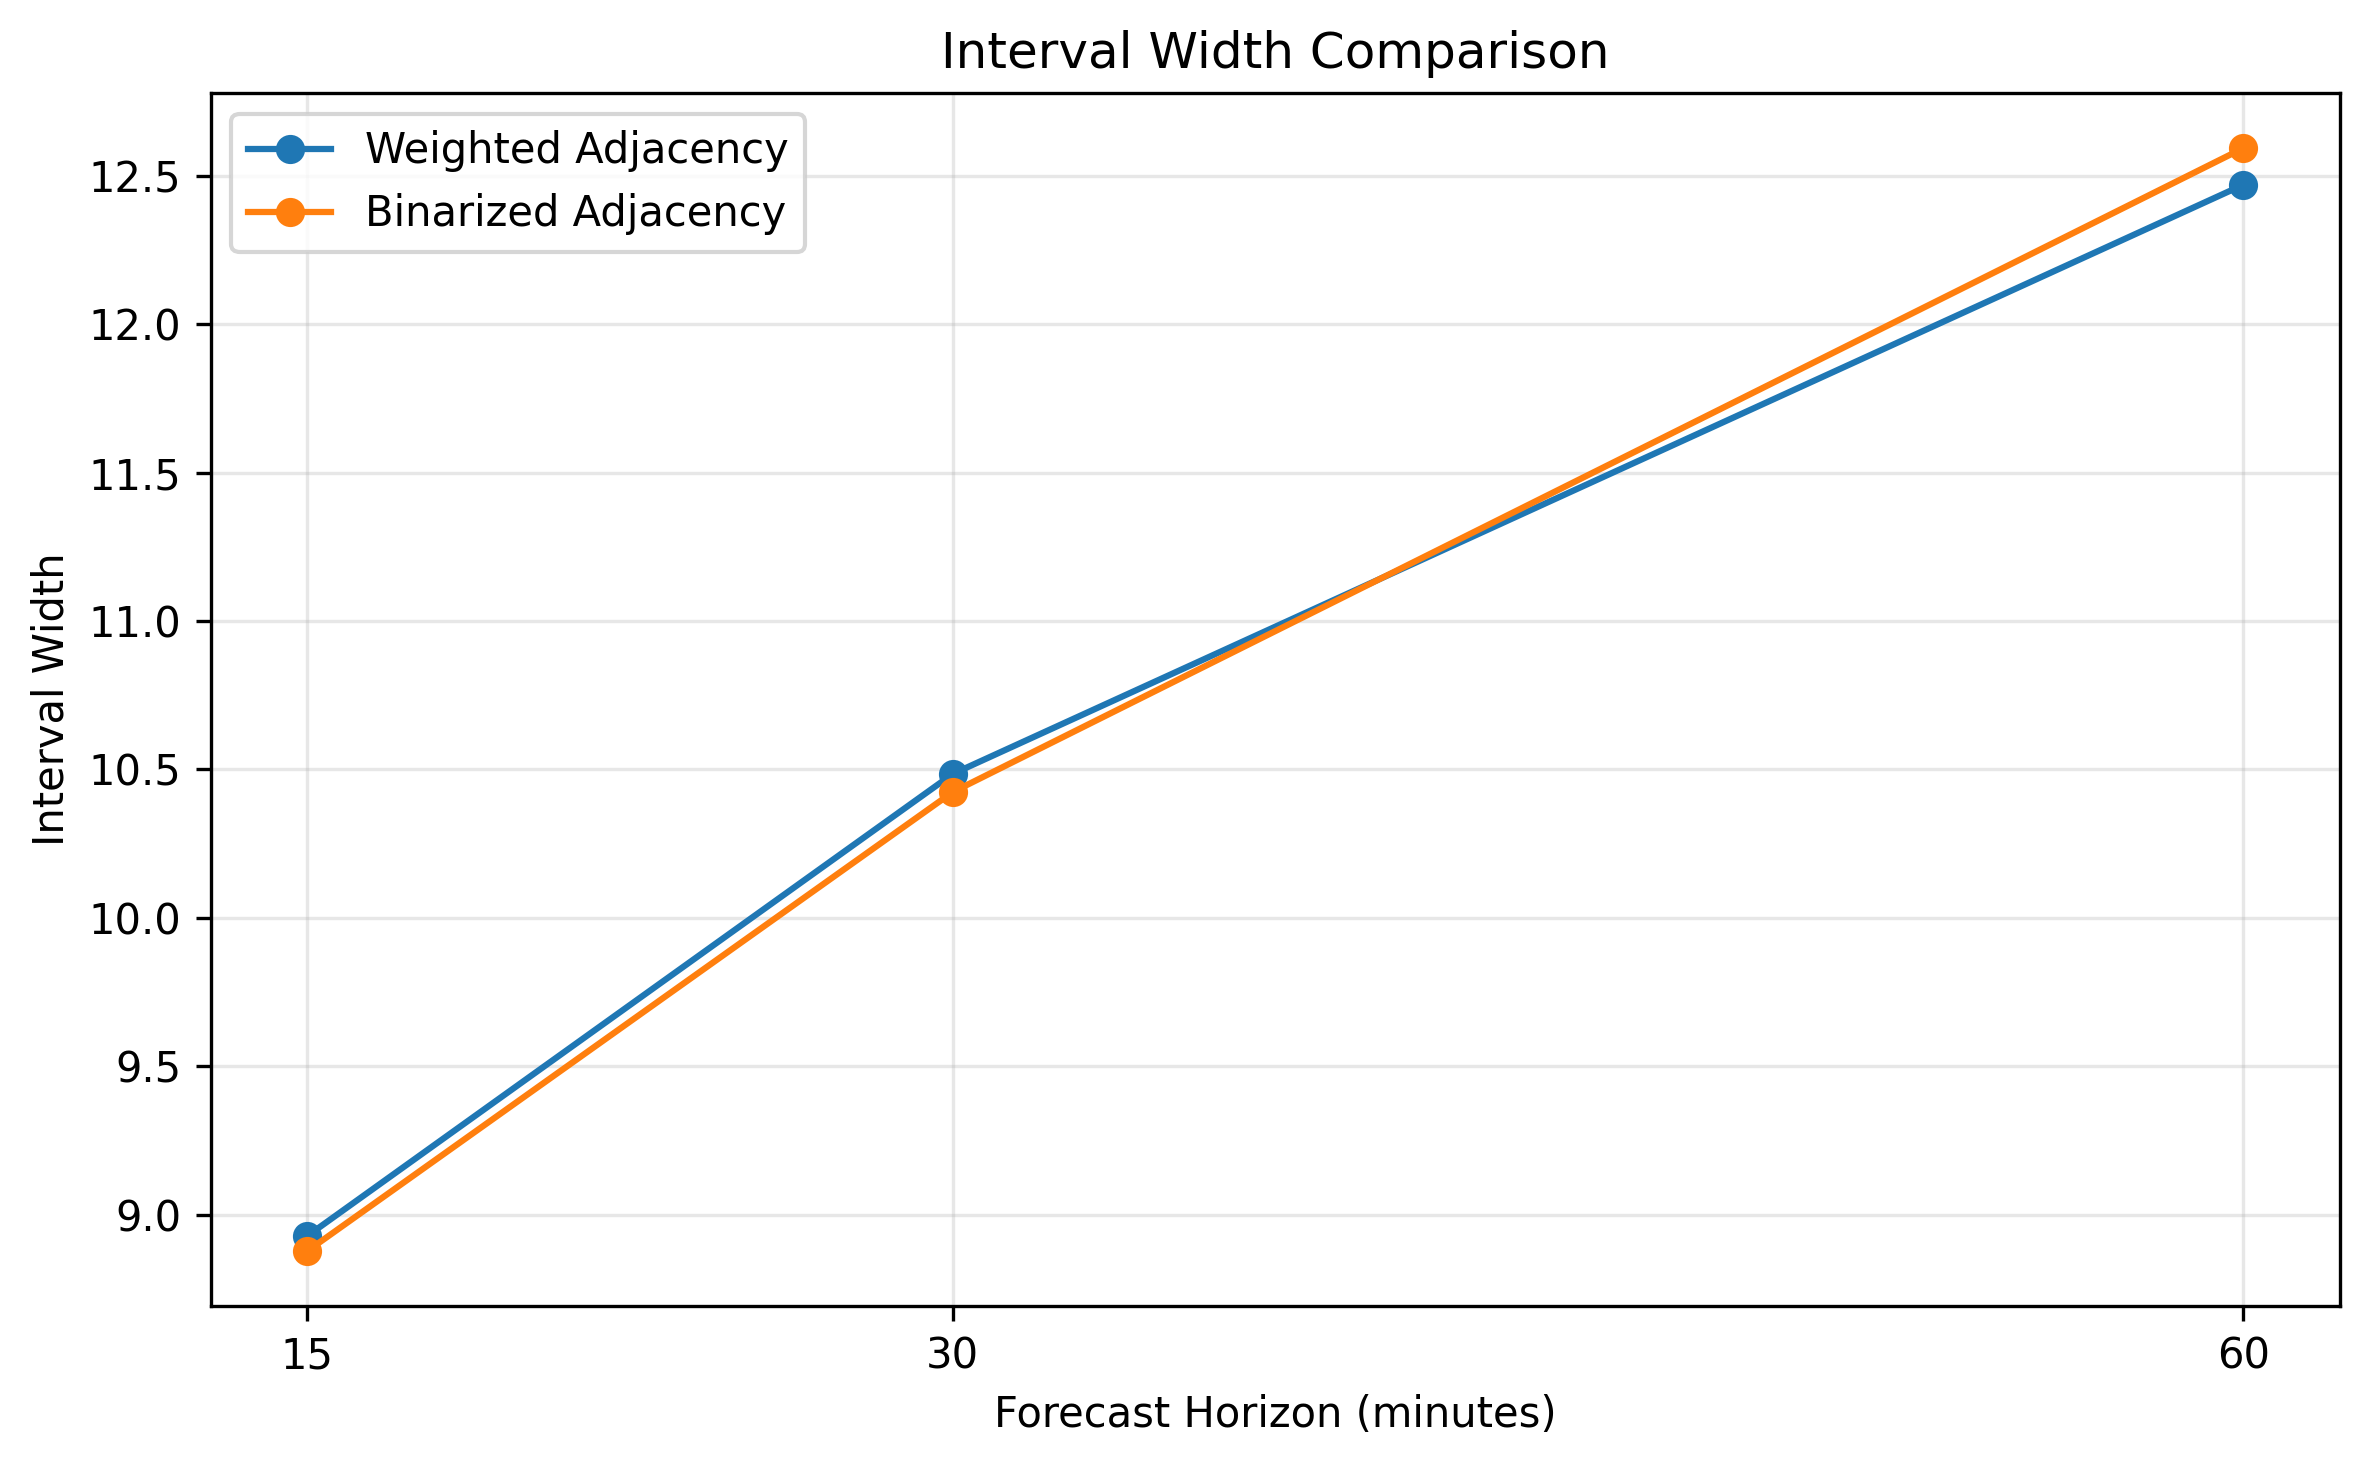
\includegraphics[width=\linewidth]{img/graph_temporal/ablation_comparison/interval_width_graph_temporal_variant_comparison}
    \end{minipage}

    \caption{Comparison of the Graph-Temporal model using the weighted and
    binary adjacency matrices. The top row reports point forecasting
    performance in terms of MAE (left) and RMSE (right), while the bottom
    row reports empirical coverage (left) and prediction interval width
    (right) across the three forecasting horizons.}
    \label{fig:weighted_binary_comparison}
\end{figure}

The comparison is further illustrated in
Figure~\ref{fig:weighted_binary_comparison}. The probabilistic results reveal
a more nuanced difference. At 15 and 30 minutes, the binary graph produces
slightly narrower intervals, while its empirical coverage is slightly closer
to the nominal 80\% level. At 60 minutes, however, the binary representation
produces a slightly wider interval, while coverage remains almost unchanged.
Therefore, binarizing the graph does not provide a consistent advantage in
terms of interval sharpness or reliability.

The probabilistic metrics provide further evidence in favor of preserving
the original edge weights. The weighted graph achieves lower Pinball Loss
for all three predicted quantiles and at every forecasting horizon. The
difference also becomes more pronounced at longer horizons, consistently
with the behavior observed for MAE and RMSE. This indicates that the edge
weights contribute not only to point forecasting accuracy, but also to the
estimation of the predictive quantiles.


Overall, these results indicate that the benefit of graph message passing is
not determined solely by the presence of connections between sensors. The
relative edge weights provide useful information for spatial aggregation,
with their contribution becoming more evident as the forecasting horizon
increases. Since the binary graph does not provide a consistent improvement
in probabilistic reliability and results in higher point errors,
the original weighted adjacency matrix was retained for the main
Graph-Temporal model.


\section{Robustness under Distribution Shift}
\label{sec:distribution_shift}

The previous experiments evaluate forecasting performance over the complete
test distribution. However, average performance may hide substantial
degradation under traffic conditions that are less frequently represented
during training. To investigate this aspect, the Graph-Temporal model is
evaluated under a predefined high-congestion stress condition. The stress
condition is defined exclusively from the training data, preventing
information from the validation or test sets from influencing the definition
of the shifted subset.

\subsection{High-Congestion Definition}
\label{subsec:congestion_definition}

High-congestion conditions are identified using sensor-specific speed
thresholds. For each sensor $n$, a congestion threshold $\tau_n$ is defined
as the 10th percentile of its valid speed observations in the training set,

\begin{equation}
    \tau_n =
    Q_{0.10}
    \left(
        \left\{y_{t,n}^{\mathrm{train}} :
        m_{t,n}^{\mathrm{train}} = 1\right\}
    \right),
    \label{eq:sensor_congestion_threshold}
\end{equation}

where $m_{t,n}^{\mathrm{train}}$ denotes the availability mask. A sensor is
therefore considered congested at time $t$ when its valid observed speed is
lower than or equal to its sensor-specific threshold. Using a separate
threshold for each sensor accounts for the different typical speed ranges
observed across locations in the road network.

The network-level congestion ratio at timestamp $t$ is then defined as the
fraction of valid sensors that are classified as congested,

\begin{equation}
    C_t =
    \frac{
        \sum_{n=1}^{N}
        m_{t,n}\,
        \mathbb{I}\!\left(y_{t,n} \leq \tau_n\right)
    }{
        \sum_{n=1}^{N} m_{t,n}
    },
    \label{eq:congestion_ratio}
\end{equation}

where $\mathbb{I}(\cdot)$ is the indicator function. This definition measures
the spatial extent of congestion at each timestamp rather than relying on the
speed of a single sensor.

Finally, the threshold used to identify a high-congestion event is defined
as the 95th percentile of the congestion ratios observed in the training
set,

\begin{equation}
    \tau_{\mathrm{peak}}
    =
    Q_{0.95}
    \left(
        \left\{C_t^{\mathrm{train}}\right\}
    \right).
    \label{eq:peak_threshold}
\end{equation}

For the METR-LA training partition, this procedure yields
$\tau_{\mathrm{peak}} = 0.3495$. Consequently, a timestamp is classified as
a high-congestion condition when at least approximately 35\% of the valid
sensors simultaneously exhibit speeds below their respective training-based
10th-percentile thresholds.

\begin{figure}[t]
    \centering
    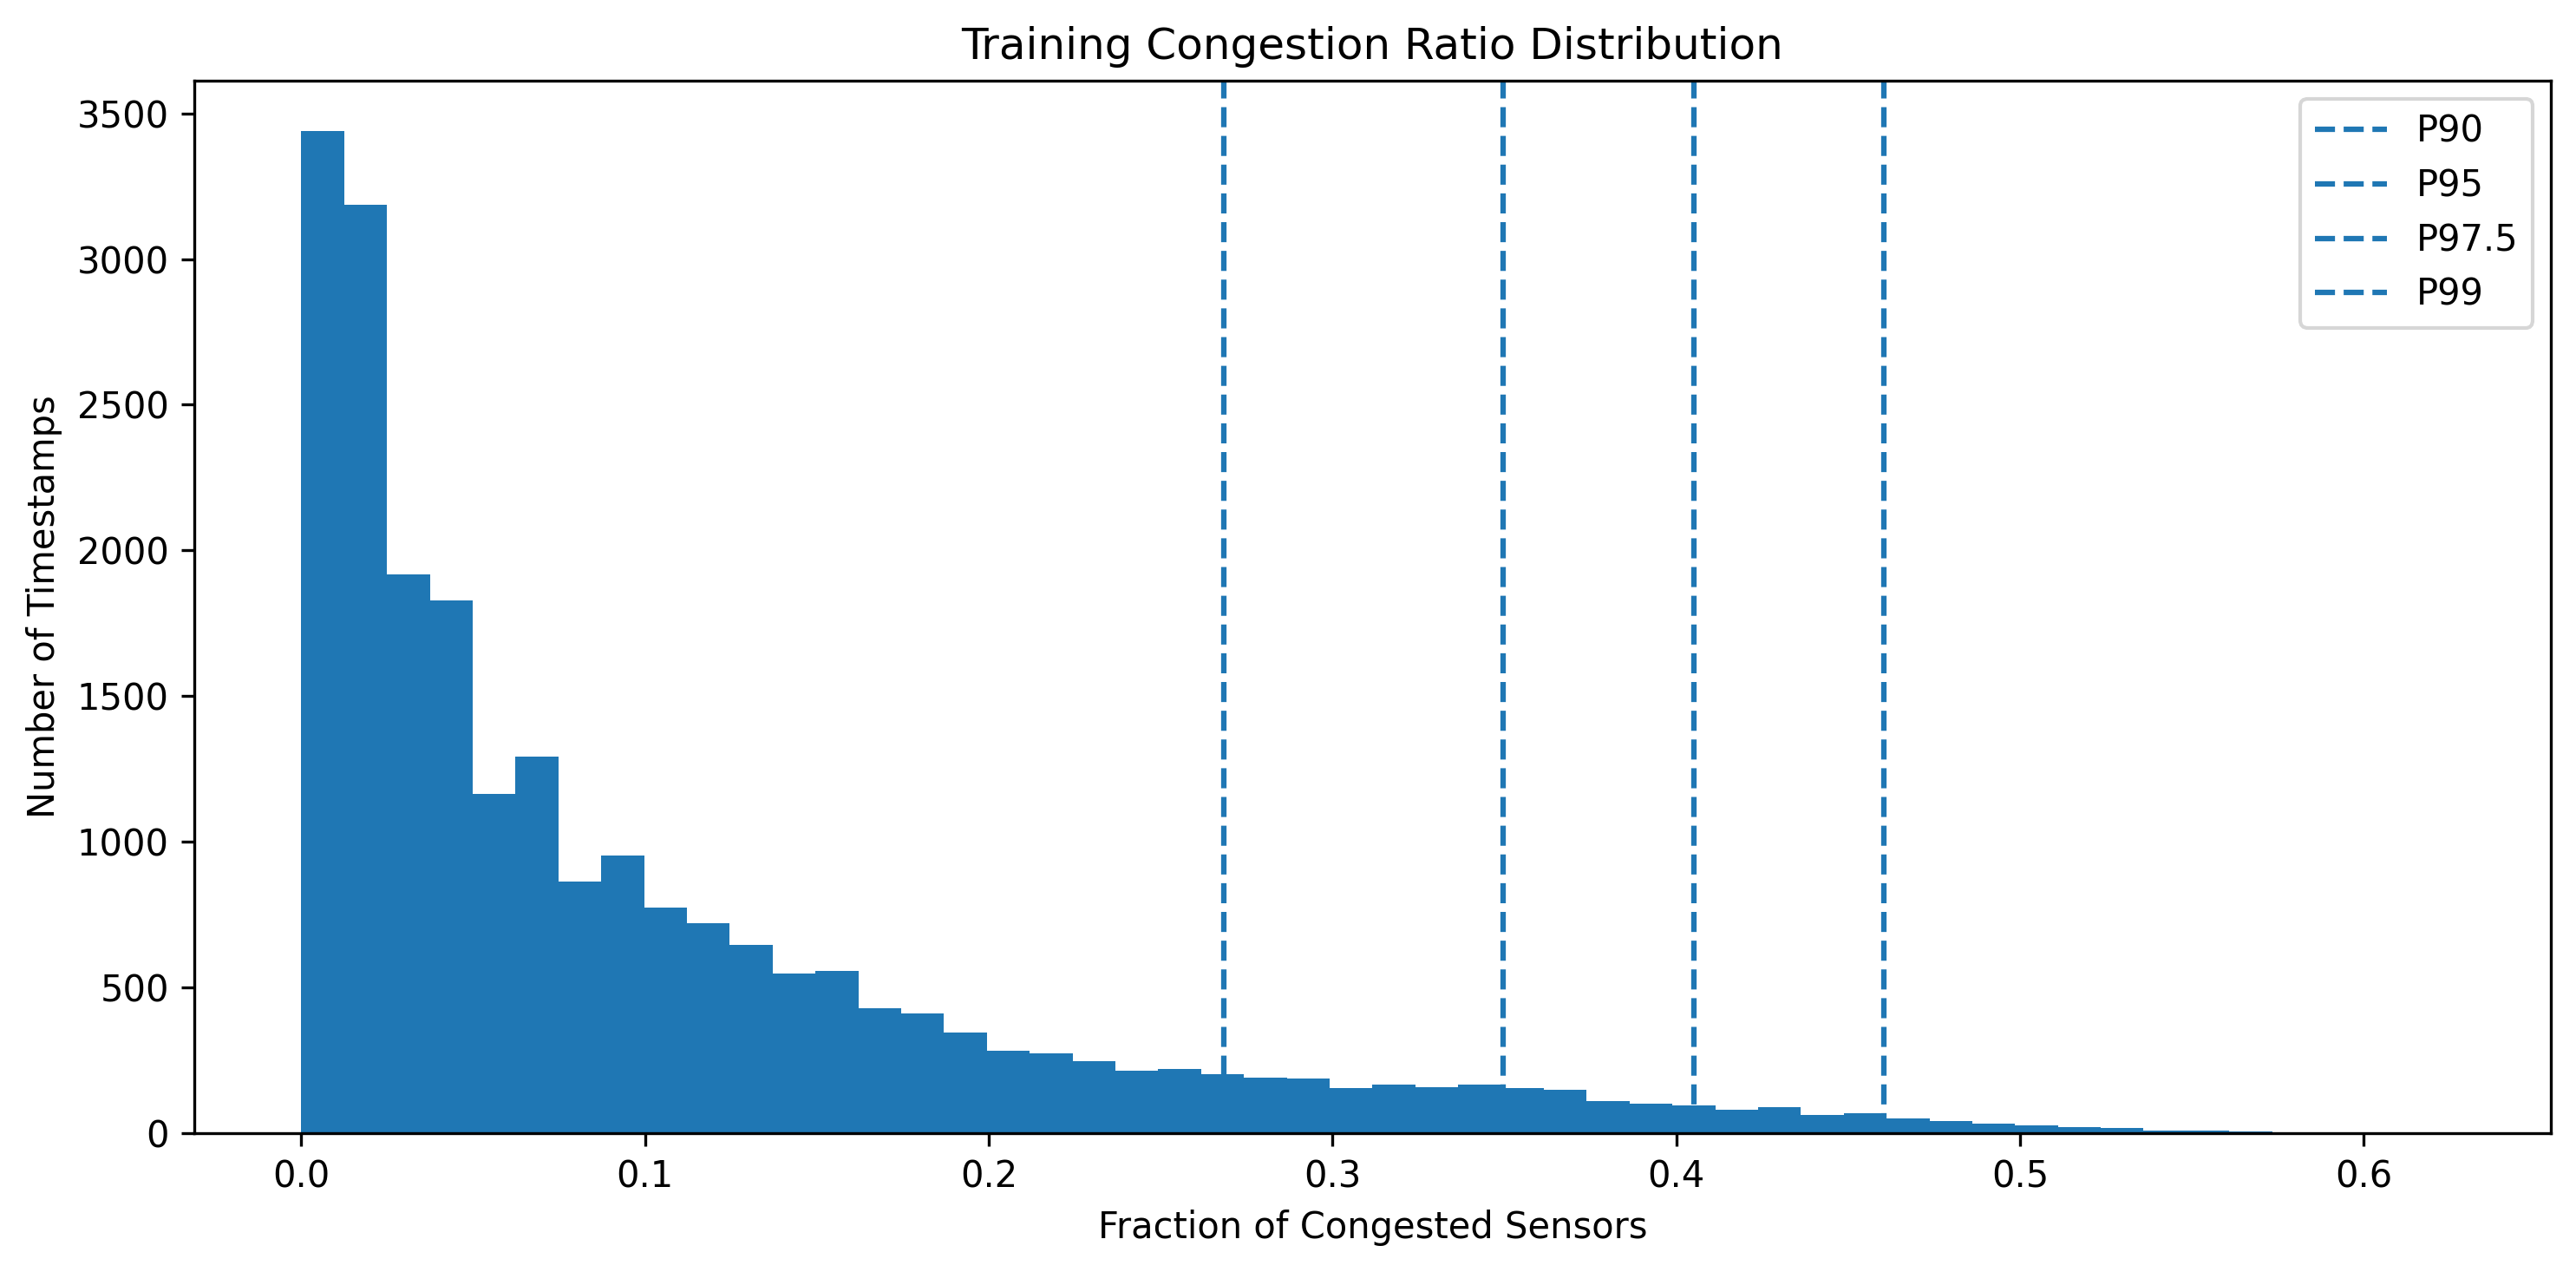
\includegraphics[width=0.75\linewidth]
    {img/distribution_shift/congestion_ratio_distribution}
    \caption{Distribution of the network-level congestion ratio $C_t$ in the
    training set.}
    \label{fig:congestion_ratio_distribution}
\end{figure}

Figure~\ref{fig:congestion_ratio_distribution} shows the training
distribution used to define the stress condition. By selecting its 95th
percentile, the stress test focuses on relatively uncommon periods in which
congestion simultaneously affects a substantial fraction of the network.
Importantly, both the sensor-specific thresholds $\tau_n$ and the
network-level threshold $\tau_{\mathrm{peak}}$ are estimated exclusively
from the training partition and subsequently kept fixed when classifying
validation and test observations.


\subsection{Stress-Test Protocol}
\label{subsec:stress_protocol}

The high-congestion definition introduced in
Section~\ref{subsec:congestion_definition} is applied to the forecasting
targets of each test window. Since the model is evaluated at three different
forecasting horizons, congestion is assessed independently at the target
timestamp corresponding to each horizon.

More specifically, for a test sample whose input sequence ends at time $t$,
the congestion condition for forecasting horizon $h$ is determined from the
network-level congestion ratio at the corresponding future timestamp
$t+h$. The sample is classified as high congestion for horizon $h$ when

\begin{equation}
    C_{t+h} \geq \tau_{\mathrm{peak}},
    \label{eq:high_congestion_sample}
\end{equation}

where $\tau_{\mathrm{peak}}=0.3495$ is the threshold estimated exclusively
from the training partition. Otherwise, the sample is assigned to the normal
subset for that horizon.

This horizon-specific classification is necessary because traffic conditions
may change within the 60-minute forecasting window. Consequently, the same
input window can be classified as normal at one forecasting horizon and as
high congestion at another. The stress-test subsets for 15, 30, and
60 minutes should therefore be interpreted independently rather than as a
single fixed set of test windows.

Applying this procedure to the 6224 test windows yields 484 high-congestion
samples and 5740 normal samples at each evaluated horizon. Although the
subset sizes are identical, their composition differs across horizons. For
example, the high-congestion masks have a Jaccard similarity of 0.741 between
15 and 30 minutes, 0.579 between 30 and 60 minutes, and 0.449 between
15 and 60 minutes. This decreasing overlap is expected because the target
timestamps become progressively farther apart.

The stress test evaluates the same trained Graph-Temporal model used in the
previous experiments, without retraining or adapting it to high-congestion
conditions. Forecasting metrics are computed separately over the normal and
high-congestion subsets using the target availability mask. This allows the
degradation associated with the shifted traffic condition to be measured
while keeping the model, preprocessing pipeline, and evaluation procedure
unchanged.

\subsection{Quantitative Results}
\label{subsec:shift_quantitative}

Table~\ref{tab:congestion_results} reports the performance of the
Graph-Temporal model separately under normal and high-congestion conditions.
A substantial degradation is observed under high congestion at all three
forecasting horizons, and the difference becomes progressively larger as the
prediction horizon increases.

\begin{table}[t]
    \centering
    \caption{Performance of the Graph-Temporal model under normal and
    high-congestion conditions on the test set.}
    \label{tab:congestion_results}
    \resizebox{\linewidth}{!}{
    \begin{tabular}{llrrrrrrrr}
        \toprule
        Condition & Horizon &
        MAE & RMSE &
        Pinball$_{0.1}$ & Pinball$_{0.5}$ & Pinball$_{0.9}$ &
        Coverage (\%) & Interval Width \\
        \midrule
        Normal
        & 15 min & 2.770 & 5.289 & 0.819 & 1.385 & 0.559 & 78.4 & 8.499 \\
        & 30 min & 3.257 & 6.453 & 0.990 & 1.629 & 0.626 & 78.3 & 9.911 \\
        & 60 min & 3.974 & 7.957 & 1.266 & 1.987 & 0.705 & 78.3 & 11.730 \\
        \midrule
        High congestion
        & 15 min & 4.463 & 7.669 & 1.159 & 2.232 & 1.044 & 78.7 & 14.035 \\
        & 30 min & 5.636 & 9.660 & 1.467 & 2.818 & 1.281 & 77.9 & 17.283 \\
        & 60 min & 7.414 & 12.296 & 1.957 & 3.707 & 1.596 & 75.8 & 21.169 \\
        \bottomrule
    \end{tabular}}
\end{table}

It is worth noting that the performance observed under normal conditions is
close to the overall test performance reported in
Section~\ref{sec:in_distribution_results}. This is expected from the
definition of the stress condition. High congestion is intentionally defined
as a relatively rare event through the 95th percentile of the training
congestion-ratio distribution and accounts for only 484 out of 6224 test
windows, approximately 7.8\%, at each forecasting horizon. Consequently,
the overall test metrics are dominated by the much larger normal subset and
can therefore conceal the substantially poorer performance observed during
high-congestion periods.

\begin{figure}[t]
    \centering

    % First row: point forecasting metrics
    \begin{minipage}[b]{0.48\linewidth}
        \centering
        
\includegraphics[width=\linewidth]
        {img/distribution_shift/mae_distribution_shift}
    \end{minipage}
    \hfill
    \begin{minipage}[b]{0.48\linewidth}
        \centering
        
\includegraphics[width=\linewidth]
        {img/distribution_shift/rmse_distribution_shift}
    \end{minipage}

    \vspace{0.4cm}

    % Second row: probabilistic metrics
    \begin{minipage}[b]{0.48\linewidth}
        \centering
        
\includegraphics[width=\linewidth]
        {img/distribution_shift/coverage_distribution_shift}
    \end{minipage}
    \hfill
    \begin{minipage}[b]{0.48\linewidth}
        \centering
        
\includegraphics[width=\linewidth]
        {img/distribution_shift/interval_width_distribution_shift}
    \end{minipage}

    \caption{Performance of the Graph-Temporal model under normal and
    high-congestion conditions. The top row compares MAE (left) and RMSE
    (right), while the bottom row reports empirical coverage (left) and
    prediction interval width (right) across the three forecasting horizons.}
    \label{fig:congestion_performance}
\end{figure}

The degradation in point forecasting accuracy is clearly visible in
Figure~\ref{fig:congestion_performance}. At 15 minutes, MAE increases from
2.770 under normal conditions to 4.463 under high congestion, corresponding
to an increase of approximately 61\%. The difference becomes larger at
longer horizons: MAE increases from 3.257 to 5.636 at 30 minutes and from
3.974 to 7.414 at 60 minutes, corresponding to increases of approximately
73\% and 87\%, respectively. RMSE exhibits the same behavior, increasing
from 5.289 to 7.669, from 6.453 to 9.660, and from 7.957 to 12.296.
These results show that forecasting becomes substantially more difficult
during network-wide congestion and that the performance degradation becomes
more pronounced as the forecasting horizon increases.

The prediction intervals respond to the increased forecasting difficulty by
becoming substantially wider under high congestion. Their average width
increases from 8.499 to 14.035 at 15 minutes, from 9.911 to 17.283 at
30 minutes, and from 11.730 to 21.169 at 60 minutes. The model therefore
captures part of the increased uncertainty associated with congested traffic
conditions rather than maintaining intervals of approximately constant width.

However, the increase in interval width is not sufficient to preserve
calibration at the longest forecasting horizon. At 15 minutes, empirical
coverage remains approximately stable, changing from 78.4\% under normal
conditions to 78.7\% under high congestion. At 30 minutes, it decreases
slightly from 78.3\% to 77.9\%. The largest degradation occurs at 60 minutes,
where coverage decreases from approximately 78.3\% to 75.8\%, despite the
prediction intervals being substantially wider.

The pronounced increase in interval width also represents a loss of
sharpness. Although wider intervals appropriately express greater predictive
uncertainty, excessively wide intervals provide a less precise and therefore
less informative characterization of future traffic conditions. Under high
congestion, the model therefore exhibits a double degradation at longer
horizons: the prediction intervals become less sharp while still failing to
achieve the nominal 80\% coverage. This indicates that the additional
uncertainty expressed by the model is not sufficient to maintain reliable
probabilistic forecasts under the shifted traffic regime.

The degradation under high congestion is also evident in the probabilistic
forecasting errors. Pinball Loss increases for all three predicted quantiles
and at every forecasting horizon, with the differences becoming larger at
longer horizons. This shows that high congestion affects not only the median
forecast, but the estimated predictive distribution more generally.

Overall, the stress test reveals two distinct effects of high-congestion
conditions. First, point forecasting errors increase substantially, showing
that these traffic regimes are more difficult to predict than normal
conditions. Second, although the model reacts to this increased difficulty
by producing wider prediction intervals, the uncertainty estimates do not
fully compensate for the degradation at longer horizons. In particular, the
combination of substantially wider intervals and lower coverage at 60 minutes
indicates residual overconfidence under distribution shift. This motivates
the calibration mitigation investigated in Section~\ref{sec:mitigation}.

\subsection{Qualitative Analysis}
\label{subsec:shift_qualitative}

The aggregate behavior observed in the stress test is further examined
through representative forecasting examples. Figure~\ref{fig:shift_examples}
compares predictions produced by the Graph-Temporal model under normal and
high-congestion conditions. The examples are intended to illustrate how the
changes in forecasting accuracy and predictive uncertainty identified in the
quantitative analysis appear at the level of individual forecasting windows.

\begin{figure}[t]
    \centering

    \begin{minipage}[b]{0.49\linewidth}
        \centering
        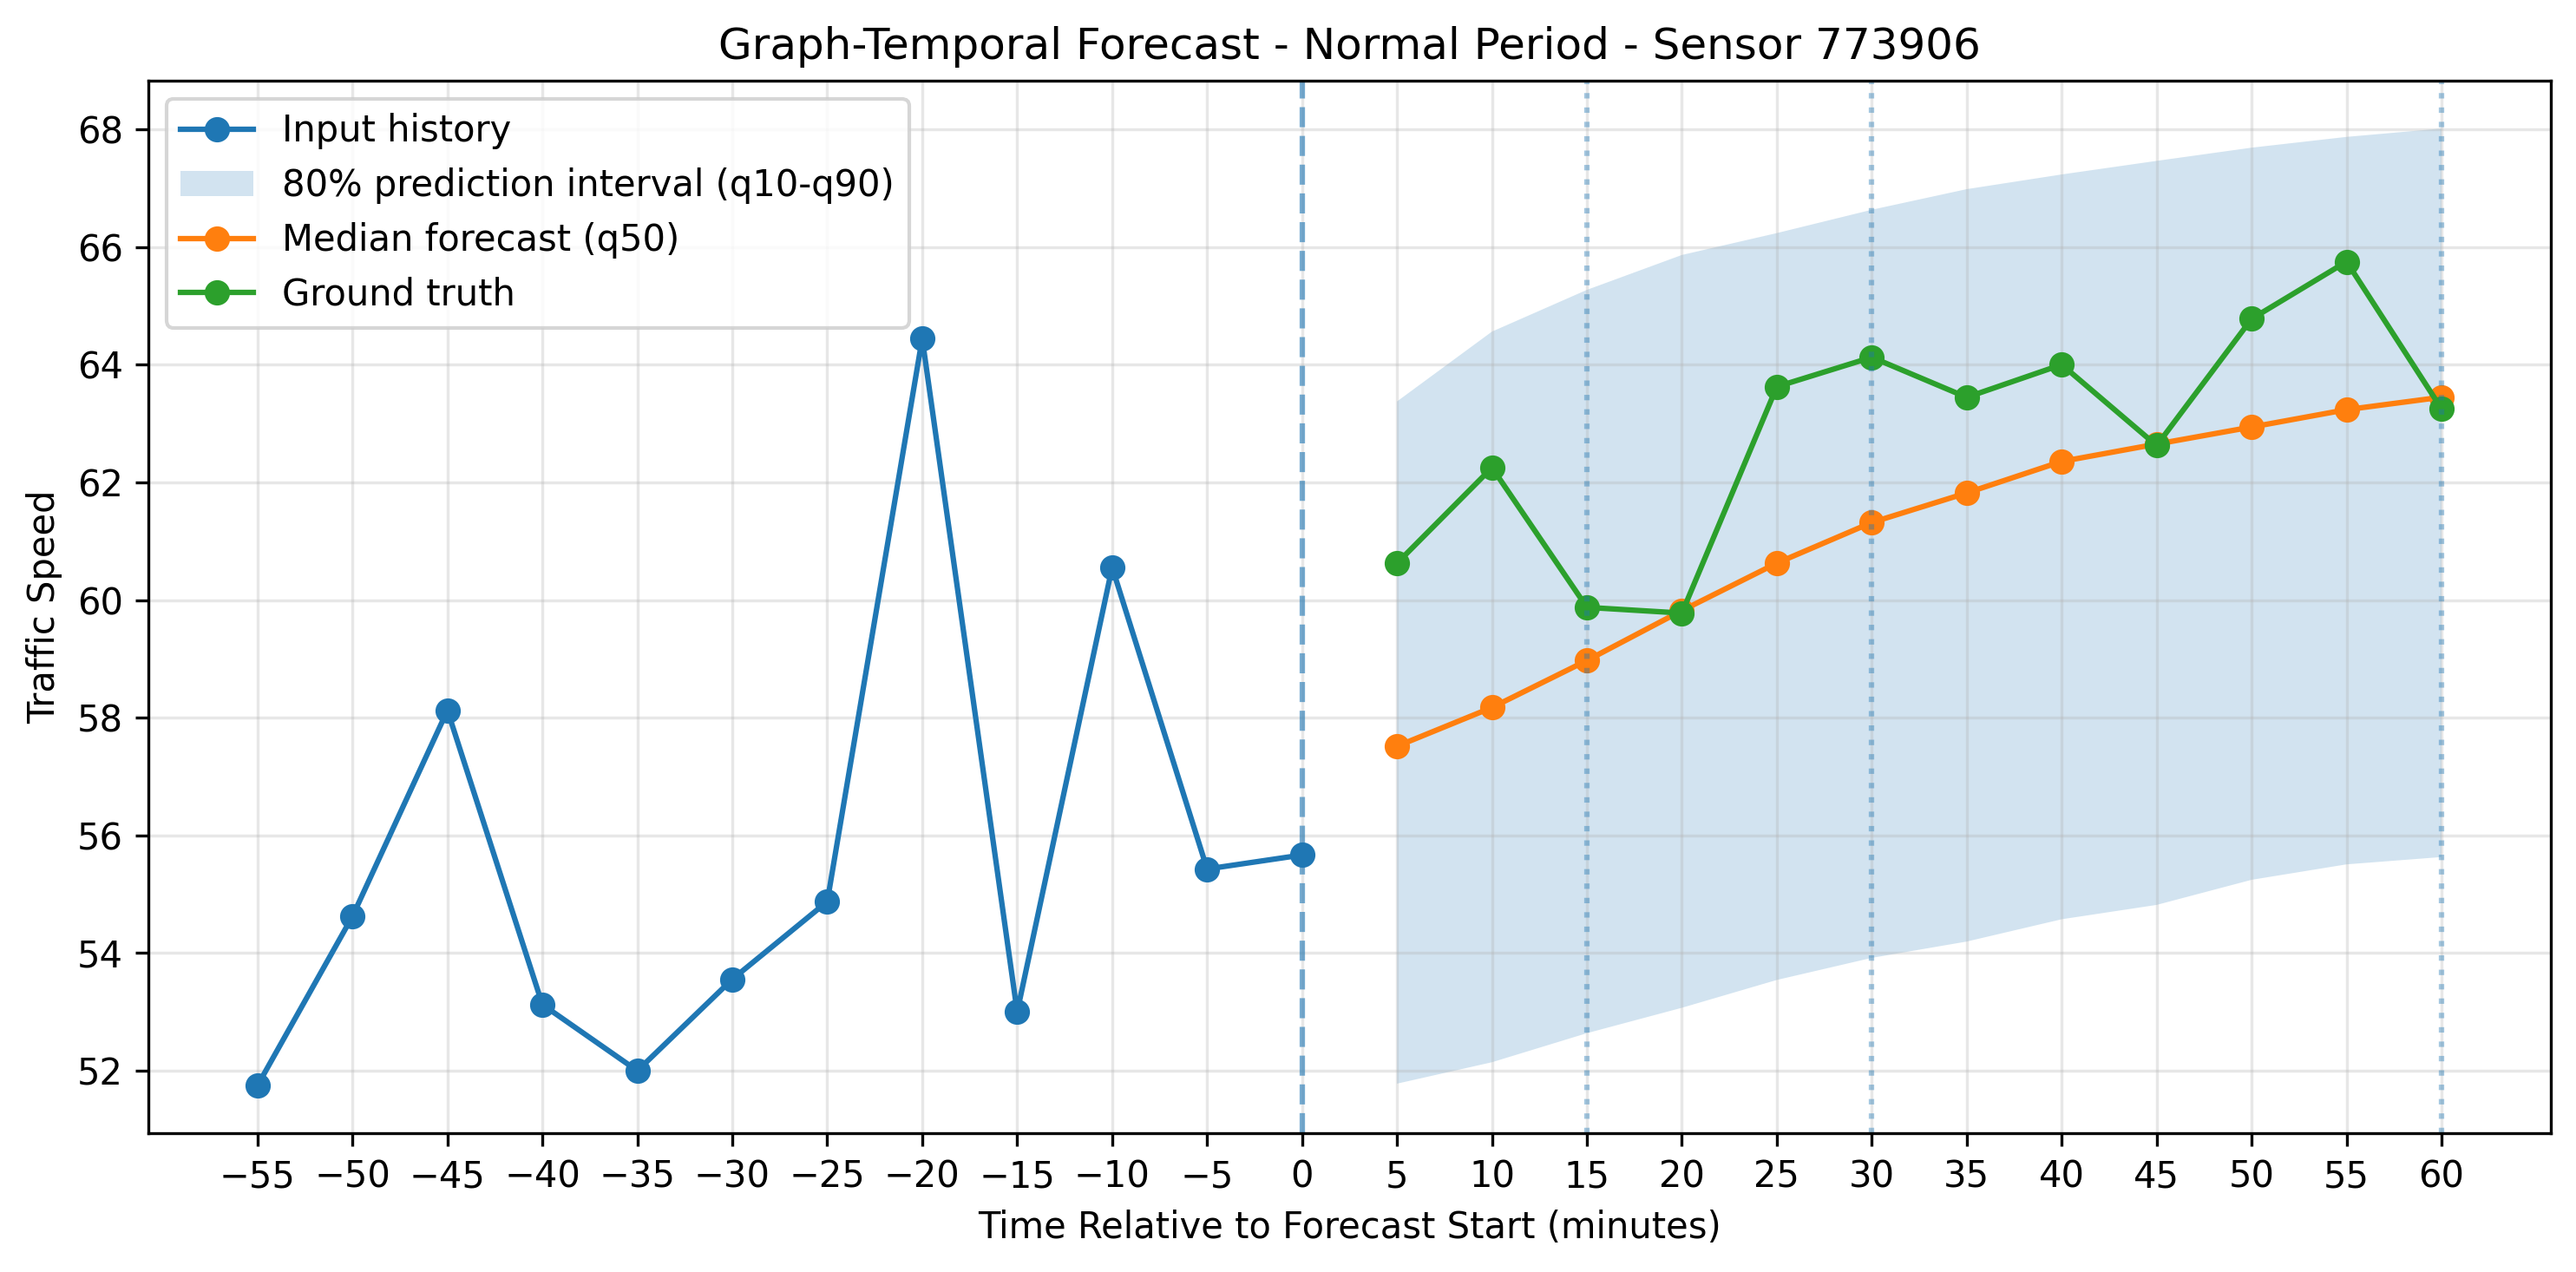
\includegraphics[width=\linewidth]
        {img/distribution_shift/normal_period}
    \end{minipage}
    \hfill
    \begin{minipage}[b]{0.49\linewidth}
        \centering
        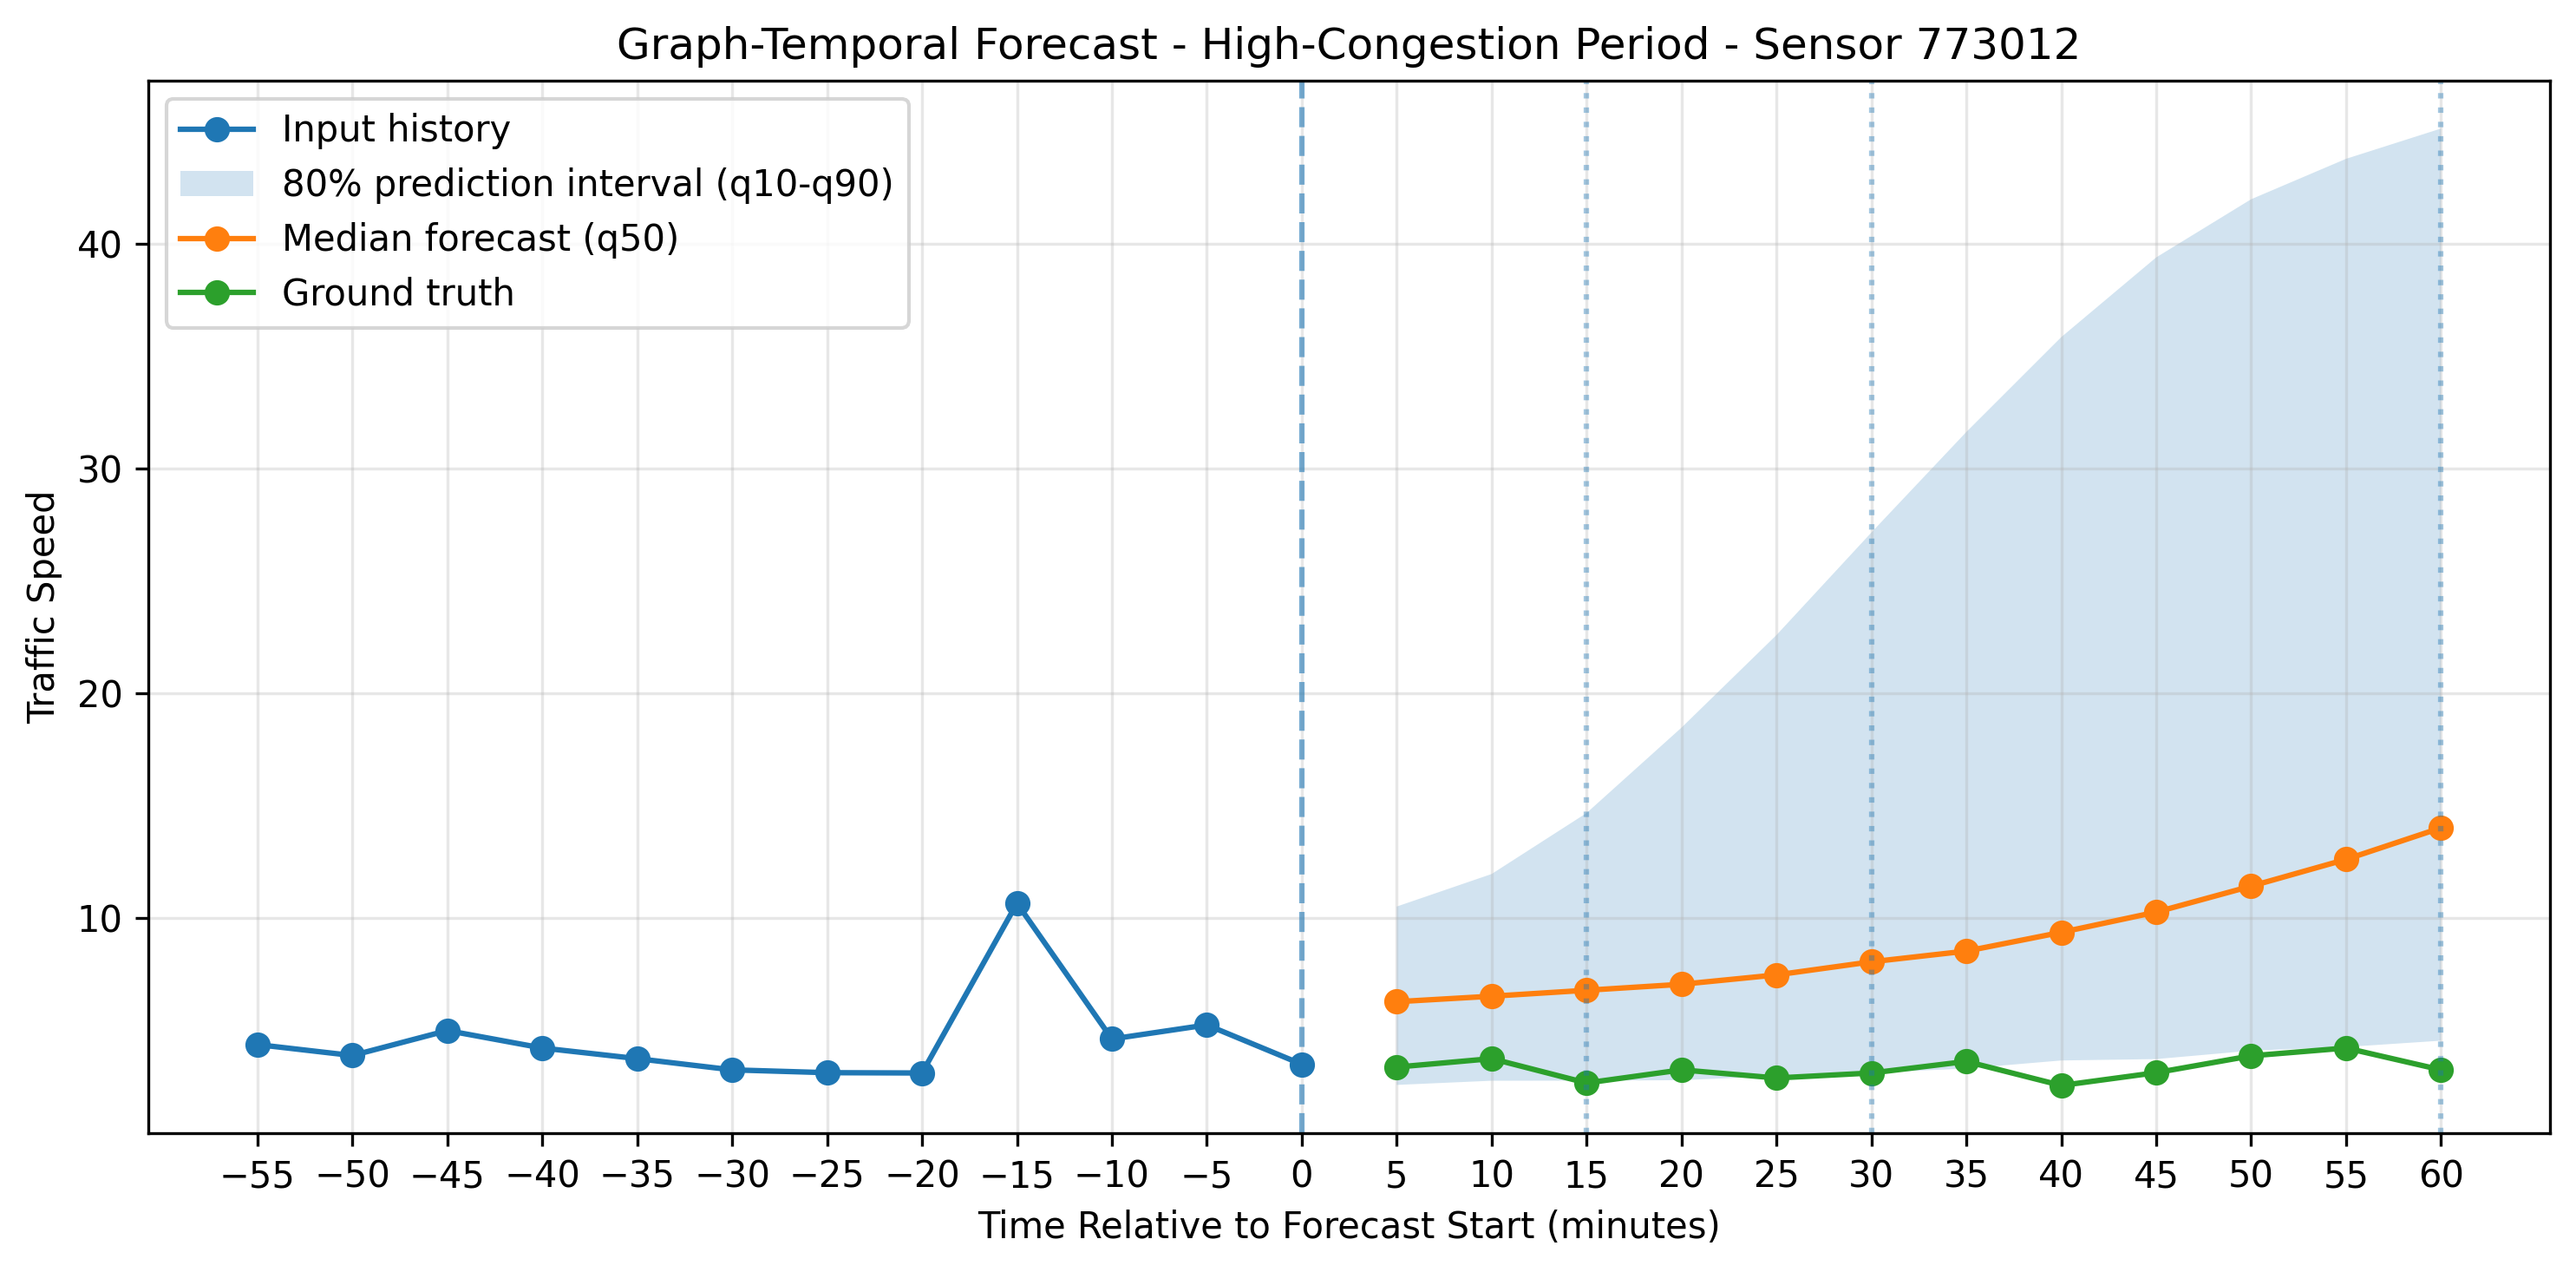
\includegraphics[width=\linewidth]
        {img/distribution_shift/high_congestion_period}
    \end{minipage}

    \caption{Representative probabilistic forecasts produced by the
    Graph-Temporal model under normal (left) and high-congestion (right)
    conditions.}
    \label{fig:shift_examples}
\end{figure}

Figure~\ref{fig:shift_examples} provides a qualitative view of how the
forecasting behavior changes between normal and high-congestion conditions.
In the normal example (left), traffic speeds remain relatively high and the
model successfully captures the increasing trend observed over the forecasting
window. Although the median forecast does not reproduce every short-term
fluctuation of the ground truth, it follows its overall evolution, while the
prediction interval remains moderately wide and contains the observed values
throughout most of the horizon.

A markedly different behavior emerges in the high-congestion example (right).
The very low observed speeds reflect a strongly congested traffic regime.
The median forecast remains relatively close to the ground truth at the
beginning of the forecasting window, but progressively overestimates future
traffic speed as the horizon increases. At the same time, the prediction
interval is substantially wider than in the normal example and expands
further toward longer horizons. This widening indicates that the model
recognizes the increasing uncertainty associated with forecasting the
evolution of the congested state. Nevertheless, the ground-truth values
remain below the lower prediction bound for most of the forecasting window.
Therefore, even though the model expresses considerably greater uncertainty,
the predictive interval is not sufficiently well positioned to cover the
actual traffic evolution.

These examples illustrate the two effects identified quantitatively in
Section~\ref{subsec:shift_quantitative}. High congestion increases the
difficulty of the point forecasting task and simultaneously leads the model
to produce wider uncertainty intervals. Although wider intervals can reflect
greater uncertainty, excessively wide intervals are also less informative,
as they provide a less precise characterization of the range of plausible
future traffic conditions. Moreover, increasing interval width alone is not
sufficient to guarantee reliable uncertainty estimates when the predictive
distribution is systematically displaced from the observations. This behavior
provides a qualitative explanation for the reduced empirical coverage
observed under high congestion, particularly at longer forecasting horizons,
and highlights the need to consider both coverage and interval sharpness when
assessing probabilistic forecasts.


\section{Mitigation Strategies}
\label{sec:mitigation}

The distribution-shift analysis showed that the Graph-Temporal model
increases the width of its prediction intervals during high-congestion
periods, but this adaptation is not sufficient to preserve the desired
coverage, particularly at the 60-minute forecasting horizon. This section
investigates a post-hoc calibration strategy designed to improve the
reliability of the probabilistic forecasts without retraining the forecasting
model. A second, training-based mitigation strategy is subsequently discussed
as a possible extension.

\subsection{Conformalized Quantile Regression}
\label{subsec:cqr}

Conformalized Quantile Regression (CQR)
\citep{romano2019cqr}
was applied as a post-hoc calibration
procedure to the prediction intervals produced by the trained Graph-Temporal
model. The method uses the validation set as a calibration set and adjusts
the lower and upper predicted quantiles according to their observed
nonconformity with respect to the ground truth. The median prediction is left
unchanged, so the procedure affects uncertainty estimation without modifying
the point forecast.

For each valid calibration target $y_i$, with predicted lower and upper
quantiles $\hat{q}_{0.1,i}$ and $\hat{q}_{0.9,i}$, the nonconformity score is
defined as

\begin{equation}
    s_i =
    \max\left(
        \hat{q}_{0.1,i} - y_i,\,
        y_i - \hat{q}_{0.9,i}
    \right).
    \label{eq:cqr_score}
\end{equation}

The score measures how far an observation lies outside the predicted
interval. Observations already contained within the interval produce
non-positive scores, whereas positive scores quantify the amount by which
the interval fails to cover the target.

The calibration scores are then used to determine how much the original
prediction intervals should be enlarged. Since the target coverage is 80\%,
the desired miscoverage level is $\alpha=0.2$. Let $n_{\mathrm{cal}}$ denote
the number of valid calibration scores. The correction $\hat{s}$ is selected
as the empirical quantile of the calibration scores at level

\begin{equation}
    q =
    \frac{\left\lceil (n_{\mathrm{cal}}+1)(1-\alpha) \right\rceil}
         {n_{\mathrm{cal}}},
    \label{eq:cqr_quantile_level}
\end{equation}

and therefore

\begin{equation}
    \hat{s}
    =
    Q_q\left(\{s_i\}_{i=1}^{n_{\mathrm{cal}}}\right).
    \label{eq:cqr_correction}
\end{equation}

Intuitively, $\hat{s}$ represents the amount by which the original interval
must be expanded so that approximately 80\% of the calibration targets are
covered.

The calibrated prediction interval for a test observation is obtained by
expanding both bounds by this correction,

\begin{equation}
    \left[
        \hat{q}_{0.1,i} - \hat{s},
        \;
        \hat{q}_{0.9,i} + \hat{s}
    \right].
    \label{eq:cqr_interval}
\end{equation}

The procedure is performed separately for each forecasting horizon, allowing
the calibration correction to reflect the different uncertainty levels at
15, 30, and 60 minutes. All calibration quantities are estimated exclusively
from the validation partition and are subsequently kept fixed during test
evaluation. Therefore, no test targets are used to determine the conformal
correction.

CQR therefore provides a lightweight mitigation strategy: it does not alter
the Graph-Temporal architecture, its learned parameters, or its median
forecast, but only recalibrates the predicted uncertainty intervals. This
makes it particularly suitable for the failure mode identified in
Section~\ref{sec:distribution_shift}, where the model already reacts to
high-congestion conditions by increasing interval width, but still exhibits
residual undercoverage.


\subsubsection{Calibration Results}
\label{subsubsec:cqr_results}

The effect of CQR is evaluated by comparing the empirical coverage and
prediction interval width before and after calibration. Table~\ref{tab:cqr_results}
reports the results for the complete test set and separately for normal and
high-congestion conditions.

\begin{table}[t]
    \centering
    \caption{Empirical coverage before and after CQR calibration under
    overall, normal, and high-congestion test conditions.}
    \label{tab:cqr_results}
    \begin{tabular}{llrr}
        \toprule
        Condition & Horizon & Before CQR (\%) & After CQR (\%) \\
        \midrule
        Overall
        & 15 min & 78.44 & 80.24 \\
        & 30 min & 78.22 & 80.14 \\
        & 60 min & 78.13 & 79.96 \\
        \midrule
        Normal
        & 15 min & 78.4 & 80.27 \\
        & 30 min & 78.3 & 80.23 \\
        & 60 min & 78.3 & 80.21 \\
        \midrule
        High congestion
        & 15 min & 78.74 & 79.89 \\
        & 30 min & 77.87 & 79.07 \\
        & 60 min & 75.81 & 77.04 \\
        \bottomrule
    \end{tabular}
\end{table}

As shown in Table~\ref{tab:cqr_results}, CQR effectively corrects the mild
undercoverage observed on the complete test distribution. Empirical coverage
increases from 78.44\%, 78.22\%, and 78.13\% to 80.24\%, 80.14\%, and
79.96\% at the 15, 30, and 60-minute horizons, respectively. The calibrated
intervals are therefore very close to the nominal 80\% coverage level across
all three forecasting horizons.

A similar behavior is observed under normal traffic conditions, where
coverage after calibration reaches 80.27\%, 80.23\%, and 80.21\%. This is
consistent with the fact that normal conditions represent the dominant
operating regime in both the calibration and test distributions. CQR is
therefore effective at correcting the systematic in-distribution
miscalibration of the original prediction intervals.

The improvement is more limited under high congestion. Coverage increases
from 78.74\% to 79.89\% at 15 minutes and from 77.87\% to 79.07\% at
30 minutes, bringing both substantially closer to the nominal level. At
60 minutes, however, coverage increases only from 75.81\% to 77.04\% and
remains clearly below the desired 80\%. Thus, the same calibration procedure
that provides nearly nominal coverage overall does not fully correct the
undercoverage observed in the most challenging shifted condition.


\begin{figure}[t]
    \centering

    \begin{minipage}[b]{0.49\linewidth}
        \centering
        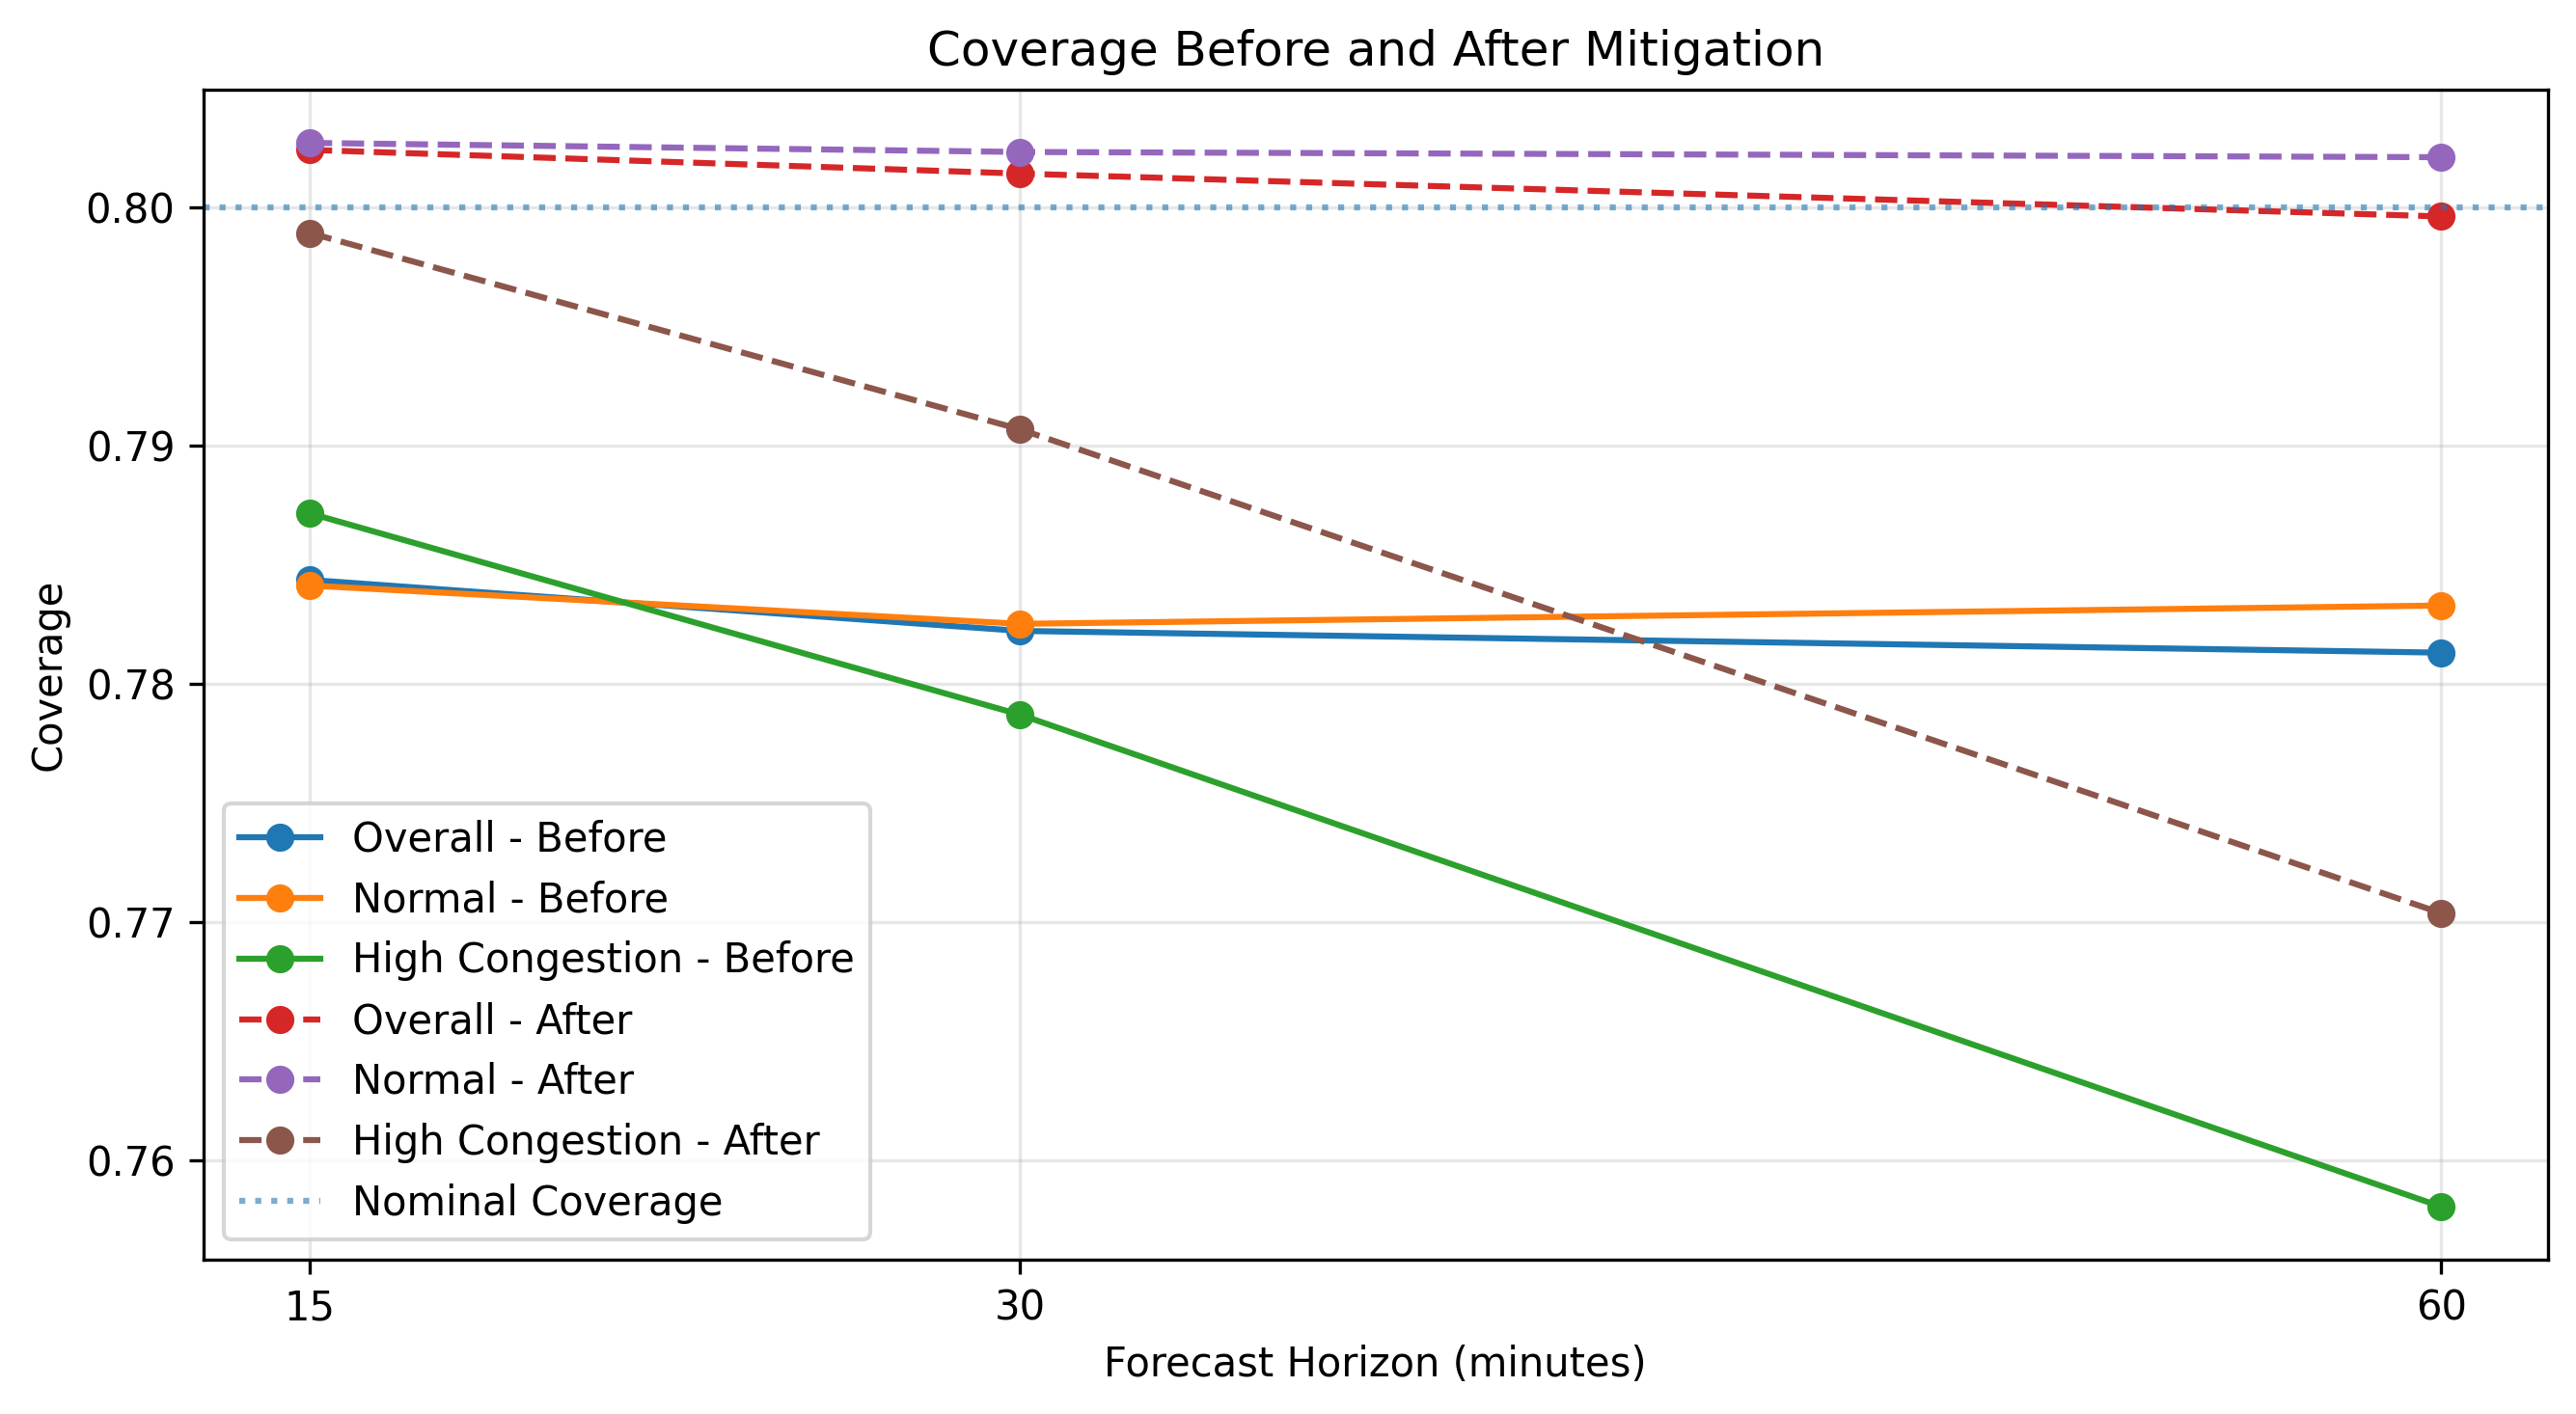
\includegraphics[width=\linewidth]{img/mitigation_strategy/coverage_mitigation_comparison}
    \end{minipage}
    \hfill
    \begin{minipage}[b]{0.49\linewidth}
        \centering
        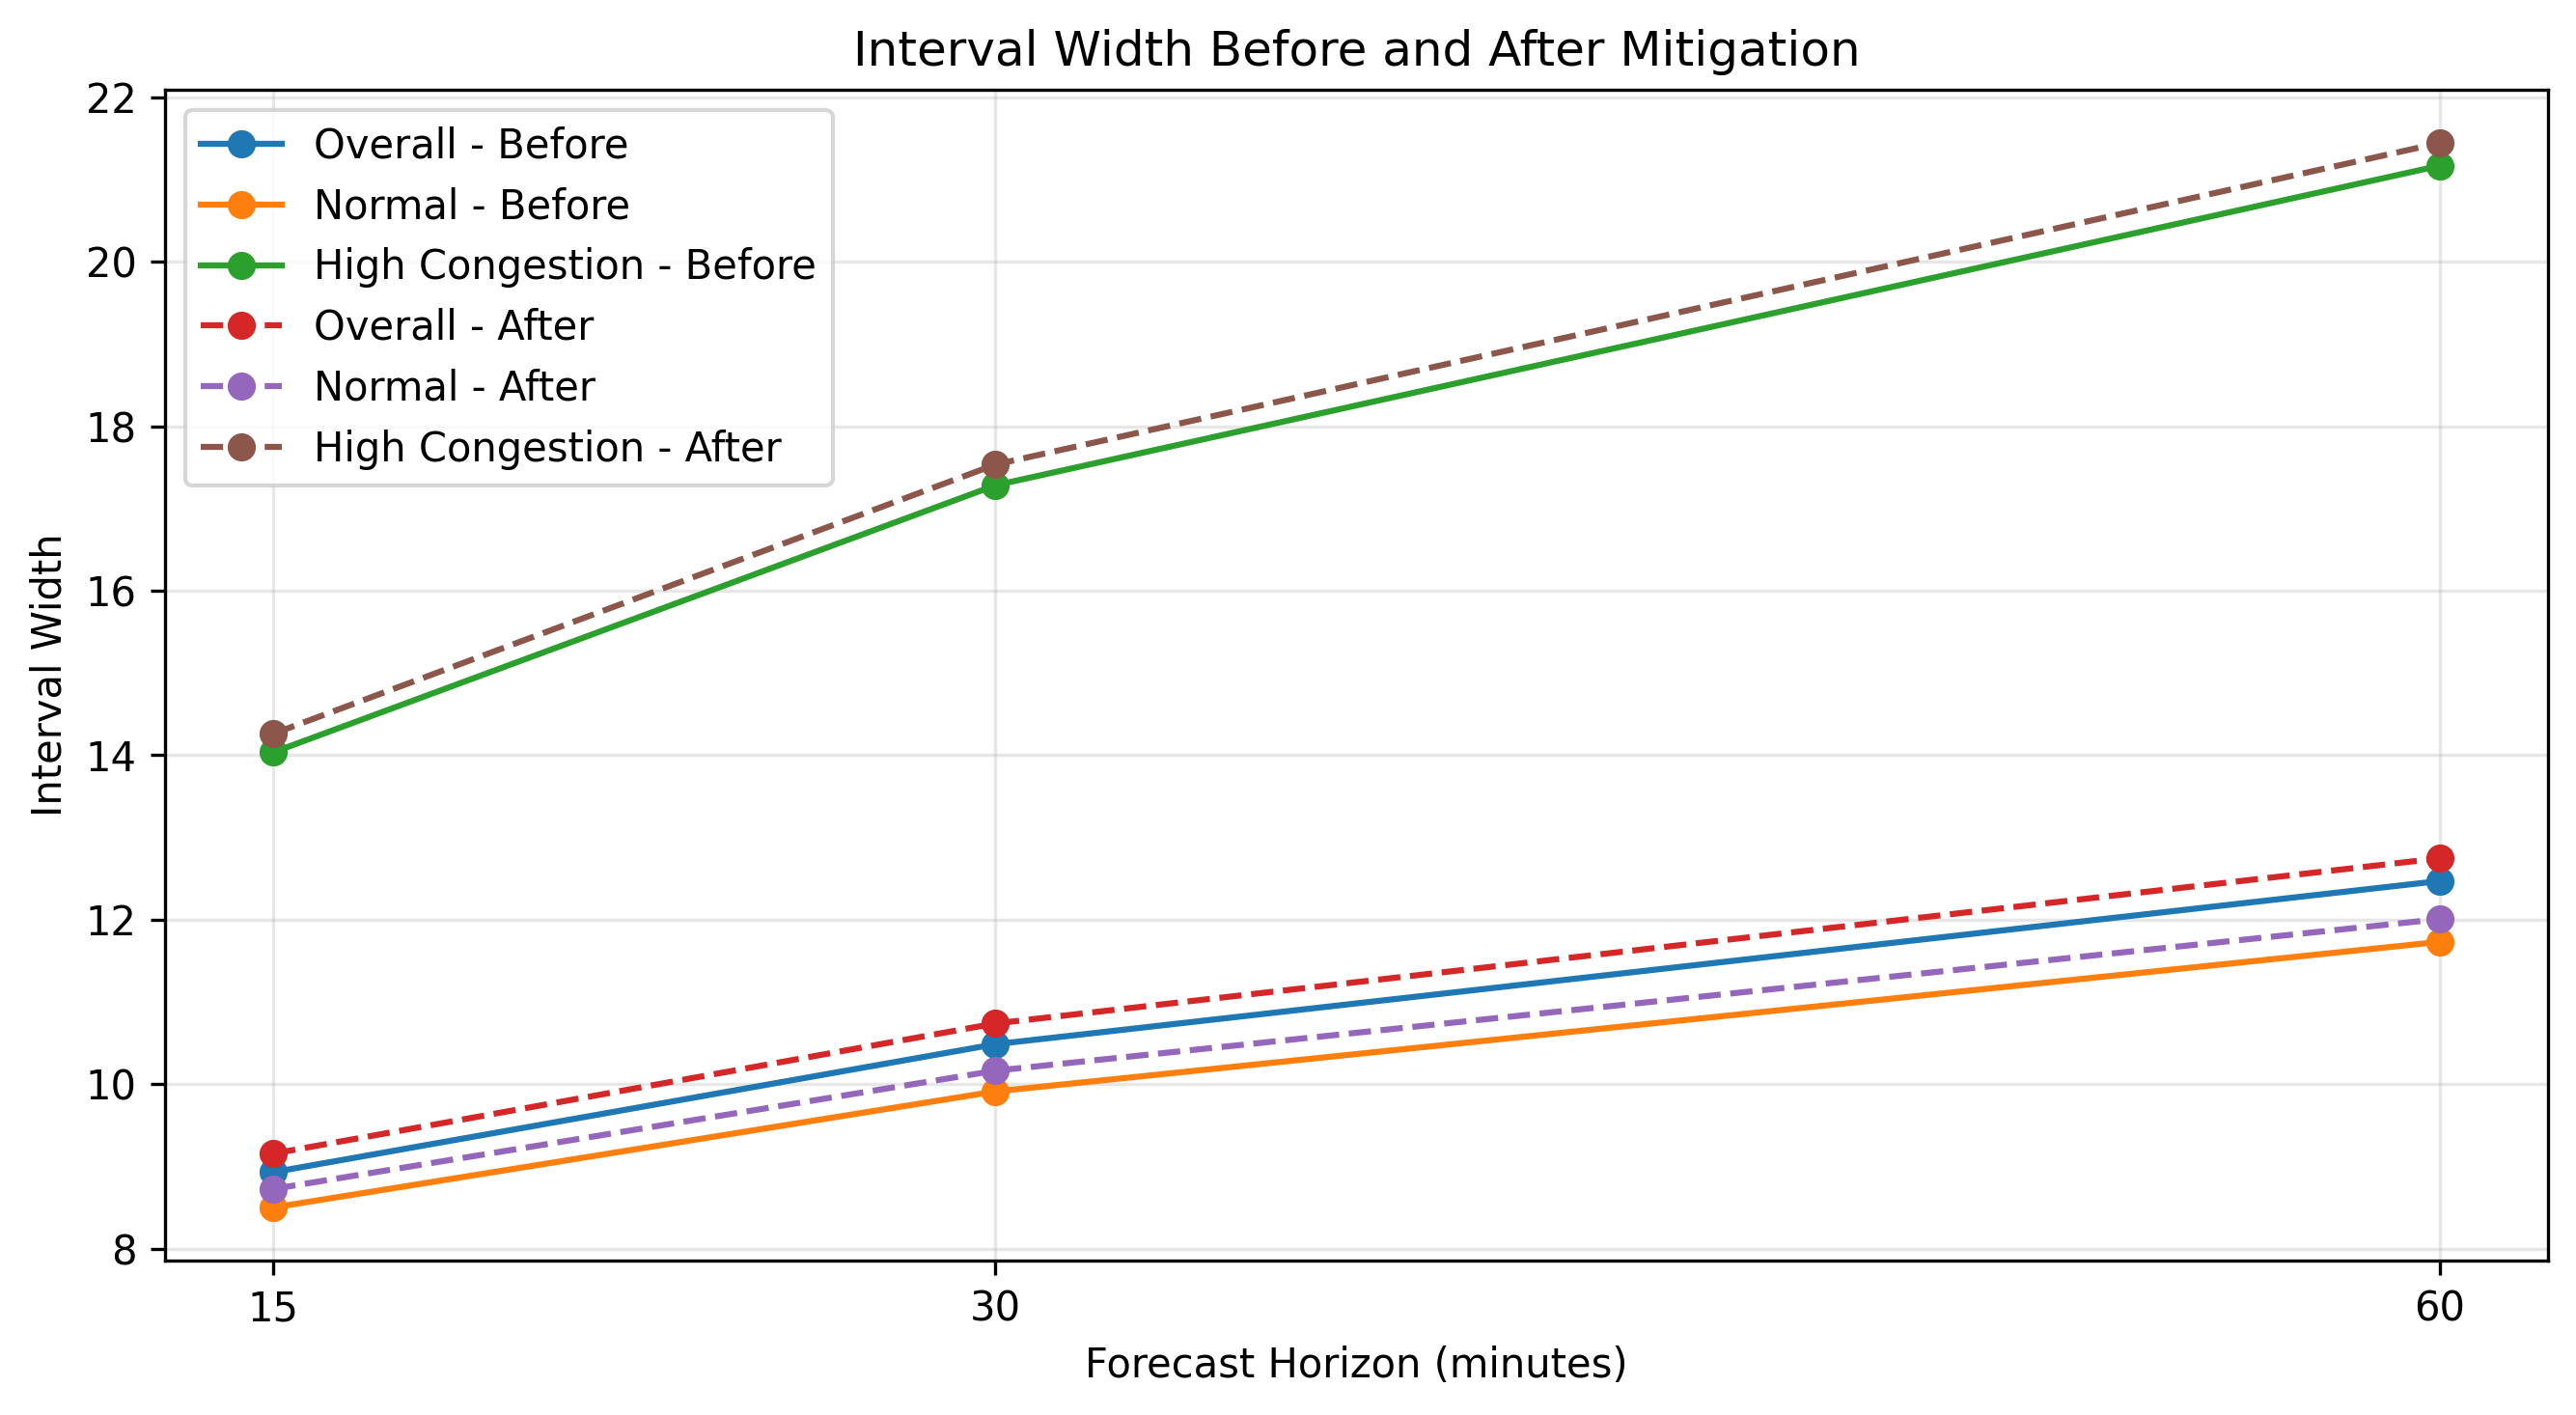
\includegraphics[width=\linewidth]{img/mitigation_strategy/interval_width_mitigation_comparison}
    \end{minipage}

    \caption{Effect of CQR calibration on empirical coverage (left) and
    prediction interval width (right) under overall, normal, and
    high-congestion conditions.}
    \label{fig:cqr_results}
\end{figure}

Figure~\ref{fig:cqr_results} shows that the improvement in coverage is
obtained by further expanding the original prediction intervals. This
introduces an important trade-off, since the intervals were already
substantially wider under high-congestion conditions. Although CQR improves
empirical coverage, the additional widening further reduces interval
sharpness and can therefore make the probabilistic forecasts less informative.
Since CQR leaves the median forecast unchanged, it does not address the
increase in point forecasting error observed under high congestion.

The remaining gap under high congestion, particularly at 60 minutes,
highlights an important limitation of the global calibration strategy.

Overall, CQR successfully mitigates the general undercoverage of the
Graph-Temporal model and substantially improves calibration under normal
conditions. It also improves coverage during high congestion, but does not
completely eliminate the reliability degradation observed at the longest
forecasting horizon. This residual failure motivates considering mitigation
strategies that explicitly account for congestion during model training.


\subsection{Congestion-Aware Training}
\label{subsec:congestion_aware}

Although CQR improves the calibration of the prediction intervals, the
remaining undercoverage under high-congestion conditions suggests that a
global post-hoc correction cannot completely address the distribution shift.
A second mitigation strategy would act directly during model training rather
than correcting the prediction intervals post hoc. In particular, previous
work on traffic speed forecasting has addressed the imbalance between
free-flow and congested conditions through congestion-adaptive loss weighting,
assigning greater importance to prediction errors occurring under congested
traffic states \citep{zhang2025casaformer}.


Following this principle, a congestion-aware extension of the probabilistic
training objective could be obtained by weighting the Pinball Loss according
to the traffic condition,

\[
\mathcal{L}_{\mathrm{CA}}
=
\frac{
\sum_{i,t,h,q}
m_{i,t,h}\,w_{i,t,h}\,
\rho_q
\left(
y_{i,t,h}-\hat{y}^{(q)}_{i,t,h}
\right)
}{
\sum_{i,t,h}m_{i,t,h}\,w_{i,t,h}
},
\]

where

\[
w_{i,t,h}
=
\begin{cases}
\lambda_{\mathrm{cong}}, &
\text{if } y_{i,t,h} \le \tau_i,\\
1, & \text{otherwise},
\end{cases}
\qquad
\lambda_{\mathrm{cong}}>1,
\]

and $\tau_i$ is the sensor-specific congestion threshold estimated from the
training data.

This would encourage the model to allocate greater optimization capacity to
the low-speed regimes in which the largest performance degradation was
observed. Unlike CQR, however, this strategy would require retraining the
forecasting model and introducing an additional weighting hyperparameter
$\lambda_{\mathrm{cong}}$. It was therefore not implemented in the present
work and is proposed as a direction for future investigation.


\section{Computational Cost and Accuracy-Reliability Trade-off}
\label{sec:cost_tradeoff}

The introduction of graph-based message passing improves forecasting accuracy,
but also increases model complexity and computational cost.
Table~\ref{tab:computational_cost} compares the Temporal model and the selected
Graph-Temporal model in terms of number of trainable parameters and training
time.

\begin{table}[t]
    \centering
    \caption{Computational cost of the Temporal and Graph-Temporal models.}
    \label{tab:computational_cost}
    \begin{tabular}{lrr}
        \toprule
        Model & Trainable Parameters & Training Time (min) \\
        \midrule
        Temporal GRU   & 40164 & 14.3 \\
        Graph-Temporal & 64868 & 34.0 \\
        \bottomrule
    \end{tabular}
\end{table}

As shown in Table~\ref{tab:computational_cost}, the Graph-Temporal model
contains 64868 trainable parameters compared with 40164 for the Temporal
model, corresponding to an increase of approximately 61.5\%. Training time also
increases from approximately 14.3 to 34.0 minutes, making the Graph-Temporal
model about 2.4 times more expensive to train in the considered experimental
setting.
This additional cost results from the repeated multi-hop graph propagation
operations and from the stacked graph-temporal blocks used to combine spatial
and temporal information.


The additional computational cost is accompanied by improved forecasting
accuracy. As shown in Section~\ref{sec:in_distribution_results}, the
Graph-Temporal model consistently outperforms the Temporal model in terms of
MAE, RMSE, and Pinball Loss, with the improvement in point forecasting
becoming more pronounced at longer horizons. It also produces sharper
prediction intervals, although with slightly lower empirical coverage.
Therefore, the accuracy gains provided by graph message passing come at the
cost of both increased computation and mild undercoverage.

Moreover, the stress-test analysis shows that this reliability gap becomes
more important under high congestion. Although the Graph-Temporal model
responds to difficult traffic conditions by producing wider intervals,
coverage decreases to 75.8\% at the 60-minute horizon. The model therefore
does not fully translate its increased uncertainty into reliable coverage
under distribution shift.

The CQR mitigation partially addresses this trade-off without increasing
model complexity or requiring retraining. Post-hoc calibration brings overall
coverage close to the nominal 80\% level while leaving the median point
forecast unchanged. Nevertheless, the remaining undercoverage under
high-congestion conditions shows that improved average calibration does not
necessarily imply equally reliable uncertainty estimates across different
traffic regimes.

Overall, the Graph-Temporal architecture provides a clear accuracy advantage
over the purely temporal baseline at the cost of greater computational
complexity. Its probabilistic forecasts are generally sharper and more
accurate in terms of quantile loss, but require additional calibration to
approach the desired coverage. The results therefore highlight that model
selection should consider not only point forecasting accuracy, but also
computational cost and the reliability of predictive uncertainty,
particularly under distribution shift.

\section{Discussion}
\label{sec:discussion}

\subsection{Main Findings}
\label{subsec:main_findings}

The experiments provide evidence that both temporal and spatial information
are relevant for traffic forecasting on METR-LA. The Temporal model already
provides a substantial improvement over persistence, showing that recent
sensor histories contain strong predictive information. Incorporating graph
message passing further improves forecasting accuracy, with the benefit
becoming more evident at longer forecasting horizons. Moreover, the
sensor-level analysis shows that this improvement is widespread across the
network, although a small number of sensors do not benefit from spatial
information.

The graph ablations further show that the way spatial information is
represented matters. Increasing the diffusion depth from $K=2$ to $K=3$
provides only limited additional benefits and introduces a less favorable
balance between error metrics, calibration, and computational cost. In
contrast, replacing the weighted adjacency matrix with a binary one produces
a clearer degradation in forecasting accuracy, particularly at longer
horizons. This suggests that the original edge weights provide useful
information beyond graph connectivity alone.

The probabilistic analysis reveals a different aspect of model performance.
The Graph-Temporal model produces sharper intervals and lower quantile losses
than the Temporal model, but its empirical coverage is slightly below the
nominal 80\% level. More importantly, this reliability degradation becomes
stronger under distribution shift. During high-congestion periods, both point
forecasting errors and prediction interval widths increase, while coverage
decreases at longer horizons. The model therefore recognizes part of the
increased uncertainty associated with congestion, but does not fully capture
the shifted predictive distribution.

Finally, the mitigation experiments show that post-hoc calibration can
substantially improve uncertainty reliability. CQR brings overall empirical
coverage close to the nominal level without modifying the median forecasts or
retraining the model. However, residual undercoverage remains under
high-congestion conditions, particularly at the longest horizon. This result
indicates that good marginal calibration does not necessarily imply equally
reliable uncertainty estimates under specific shifted conditions and
motivates mitigation strategies that explicitly account for rare traffic
regimes during training.


\subsection{Limitations}
\label{subsec:limitations}

Several limitations should be considered when interpreting the results.
First, the experiments are conducted exclusively on METR-LA and therefore
reflect the spatial structure, traffic dynamics, and missing-data patterns of
a single road network. The conclusions cannot necessarily be generalized to
other cities or sensor networks without additional evaluation.

Second, the definition of distribution shift considered in this work focuses
specifically on high-congestion periods. Although this represents a relevant
and challenging traffic regime, other forms of shift may affect forecasting
models differently, including sensor failures, changes in network topology,
or temporal changes in traffic patterns.

Third, the Graph-Temporal architecture is intentionally compact and explores
only a limited set of spatial configurations. The diffusion-depth and
adjacency ablations provide evidence about the role of graph information, but
they do not constitute an exhaustive exploration of graph neural network
architectures or graph construction strategies.

Finally, CQR is calibrated globally for each forecasting horizon using the
validation distribution. While this substantially improves marginal
coverage, it does not explicitly account for traffic regime and therefore
cannot guarantee the same calibration quality within the high-congestion
subset.


\subsection{Future Improvements}
\label{subsec:future_improvements}

Several extensions could address these limitations. A first direction would
be to evaluate the proposed congestion-aware training objective, assigning
greater importance to rare congested targets during optimization and
measuring whether this improves both point forecasts and uncertainty
estimation without substantially degrading performance under normal
conditions.

The robustness analysis could also be extended to additional distribution
shifts, such as partially masked sensor histories or simulated sensor
failures. This would provide a broader characterization of the dependence of
the Graph-Temporal model on spatial information and of its behavior when
parts of the network become unavailable.

Finally, future work could explore more expressive spatial and temporal
architectures, alternative graph construction strategies, and dynamic graphs
whose relationships evolve with traffic conditions. Evaluation on additional
traffic datasets would also be necessary to determine whether the conclusions
observed on METR-LA generalize to different road networks and traffic
regimes.


\section{Conclusion}
\label{sec:conclusion}

This work investigated probabilistic graph-based traffic forecasting under
distribution shift using the METR-LA dataset. A leakage-free experimental
pipeline was developed to compare a persistence baseline, a purely temporal
GRU, and a Graph-Temporal model combining diffusion-based message passing with
recurrent temporal modeling. In addition to point forecasting accuracy, the
analysis considered predictive uncertainty through quantile regression,
empirical coverage, and prediction interval width.

The experimental results show that incorporating the road-network graph
consistently improves forecasting accuracy over the Temporal model,
particularly at longer forecasting horizons. The graph ablations further
indicate that the weighted connectivity structure contains useful predictive
information, while increasing the diffusion depth provides only limited
additional benefits. These improvements, however, come with higher
computational cost and slightly reduced empirical coverage.

The high-congestion stress test reveals a more challenging limitation.
During congested periods, forecasting errors increase substantially and the
model responds by producing wider prediction intervals. Nevertheless,
coverage deteriorates at longer horizons, showing that increased uncertainty
does not necessarily translate into reliable uncertainty estimates under
distribution shift.

Post-hoc calibration through Conformalized Quantile Regression substantially
improves overall coverage and brings it close to the nominal 80\% level
without modifying the median forecasts or retraining the model. However, the
remaining undercoverage under high congestion shows that marginal calibration
alone is insufficient to fully address regime-specific reliability. A
congestion-aware training objective was therefore proposed as a possible
extension to explicitly increase the importance of these rare and difficult
traffic conditions during learning.

Overall, the results demonstrate the value of exploiting spatial information
for traffic forecasting while also highlighting the importance of evaluating
predictive uncertainty beyond average test performance. Reliable deployment
requires considering not only forecasting accuracy, but also calibration,
robustness to distribution shift, and the computational cost associated with
more expressive spatio-temporal models.

\bibliographystyle{plain}
\bibliography{main}

\end{document}
